\documentclass[11pt, titlepage]{article}  % , titlepage
\usepackage{Sections/Common/toshi}
%\usepackage{comment}


\begin{document}


\definecolor{labelkey}{rgb}{1,1,1}    % hide label keys
\renewcommand{\include}[1]{}
%\renewcommand\documentclass[2][]{}


\renewcommand{\thefootnote}{\fnsymbol{footnote}}
\setcounter{page}{0}
%%%%%%%%%%%%%%%%% Title page %%%%%%%%%%%%%%%%%%%%%%%%%%%%%%%%%
\thispagestyle{empty}


% paper/preprint number
\begin{flushright}
Dissertation
%RIKEN-iTHEMS-Report-?? \\
%OU-HET-???
\end{flushright}



% title
\vskip5cm%\vskip3cm
\begin{center}
{\LARGE {\bf Defects in Supersymmetric Gauge Theory  \\
\vspace{0.4cm}
and Integrable Lattice Models}}



% name
\vskip3cm%\vskip1.5cm
{\large
\bf {Toshihiro Ota} %$^{a, b}$\footnote{\href{mailto:toshihiro.ota@riken.jp}{toshihiro.ota@riken.jp}}
}



% affiliation
\vskip3cm%\vskip1cm
%\it ${}^{a}$RIKEN Interdisciplinary Theoretical \& Mathematical Sciences Program (iTHEMS), \\
%Wako, Saitama 351-0198, Japan \\
%\it ${}^{b}$
\it Department of Physics, Osaka University,  Toyonaka, Osaka 560-0043, Japan
\end{center}



%\newpage
%\vskip1cm
\begin{abstract} %abstract
    abstract
\end{abstract}



\renewcommand{\abstractname}{Acknowledgements}
\begin{abstract}
I would like to acknowledge kind support and help from many people,
without those this thesis would not have been completed.
Firstly, I would like to thank my Ph.D.~advisor Koji Hashimoto
who has given me great opportunity to start my study of string theory at Osaka university.
In particular, in the first three years of my Ph.D.~program I could learn
a lot of things through discussion and collaboration with him.
I owe deep gratitude to my collaborators Kazunobu Maruyoshi and Junya Yagi.
This thesis is largely based on the joint work with them,
and I have been enjoying discussion and chat with them every time.
They brought me to the fascinating subject at the intersection of supersymmetric gauge theory,
string theory, and integrable system.
I am also grateful to Yasuhiro Akutsu, Norihiro Iizuka, Tetsuya Onogi and Satoshi Yamaguchi
for careful reading of this thesis and giving me useful comments.

I would like to say how much of a pleasure it has been being a member of iTHEMS at RIKEN.
In particular, I really appreciate Tetsuo Hatsuda, who is the director of iTHEMS, and Masato Taki,
who was a member of iTHEMS and is also my collaborator on machine learning.
Their advice, encouragement, and arrangement were always helping me a lot during my stay at iTHEMS.
Over the past two years, I have been really benefited from stimulating discussions with
colleagues in various fields of science at iTHEMS.
Such an experience has made my Ph.D.~course quite fruitful and way more enjoyable.
I am especially indebted to mathematicians at iTHEMS; Hokuto Konno, Genki Ouchi,
Kenta Sato and Masaki Taniguchi for communicating with and telling me lots of mathematical ideas.
Inspiring discussions and interesting conversation with them were a great help of this thesis.

I would like to thank Tomoko Iwanami, Chikako Ota and Hitomi Wada, the secretaries at iTHEMS,
and Mika Umetani and Satomi Suzuki, the secretaries of the particle physics theory group
at Osaka university for arranging a lot of procedures so that I could do my research at RIKEN.
They were always kind and I was helped many times.
During my Ph.D.~study, I have been supported in part by RIKEN Junior Research Associate program and
by JSPS fellowships for Young Scientists.
Finally, I wish to thank my parents for their understanding, love and constant support.
\end{abstract}




%%%%%%%%%%%%%%%%%%%%%%%%%%%%%%%%%%%%%%%%%%%%%%%%%%%%%%%%
\renewcommand{\thefootnote}{\arabic{footnote}}
\setcounter{footnote}{0}



\vfill\eject    % newpage

\tableofcontents



\begin{comment}
\documentclass[11pt]{article}  % , titlepage
\usepackage{Common/toshi}
\begin{document}
\end{comment}



%%%%%%%%%%%%%%%%%% section 1 %%%%%%%%%%%%%%%%%%%%%%%%%%%%%%%%%
\section{Introduction}
\label{sec:intro}


Over the past decades, gauge theories have been one of the most
important subjects in theoretical physics.
They describe the fundamental interaction among elementary particles
and are building blocks of the standard model of particle physics.
Still, however, the non-perturbative dynamics of quantum gauge theories
has not been fully uncovered.

A breakthrough was initiated by the discovery of exact solutions to
the low energy effective action of certain $\CN=2$ supersymmetric gauge
theories in the pioneering works by Seiberg and Witten \cite{Seiberg:1994rs,Seiberg:1994aj}.
In their work, a Riemann surface and a differential on it, today such a pair is referred to as
``Seiberg-Witten curve'' and ``Seiberg-Witten differential,'' played a significant role, and it brought to us
rich connections to two-dimensional integrable systems \cite{Gorsky:1995zq,Martinec:1995by,Donagi:1995cf,Itoyama:1995nv}.
It was also the first time that the techniques in algebraic geometry were introduced
to theoretical physics.

The work of Seiberg and Witten was based on certain assumptions on the strong coupling
behavior of the relevant gauge theories, but it was somewhat heuristic.
Then, it was a great progress when it was shown that the mathematical description for
the prepotential conjectured by Seiberg and Witten can be obtained by an honest
calculation of the quantum corrections to a certain two-parameter
deformation of the prepotential to all orders in the instanton
expansion \cite{Nekrasov:2002qd,Nekrasov:2003rj,Nakajima:2003pg}.

Soon after these prominent works, there were two more major developments in the study of
supersymmetric gauge theories.
First, Pestun reformulated the method of supersymmetric localization \cite{Pestun:2007rz},
which generalizes previous works and allows us to exactly compute partition functions
and a class of observables for supersymmetric gauge theories on $S^4$.
Based on Pestun's result, another progress was achieved by
Alday, Gaiotto and Tachikawa \cite{Alday:2009aq}, which
is now well known as AGT correspondence.
The AGT correspondence relates four-dimensional supersymmetric gauge theories on $S^4$ and
two-dimensional (non-supersymmetric) Liouville/Toda conformal field theory.
Not only did it provide new interesting dualities among quantum field theories,
but also has promoted fruitful interactions between physicists and mathematicians.
%Involving these progresses, supersymmetric gauge theories have provide us
%many more interesting \emph{exact results}.
These interesting phenomena, involving the work of Seiberg and Witten,
can naturally be understood from the string theory viewpoint \cite{Witten:1997sc,Gaiotto:2009we}.
In addition, the techniques to compute exact physical quantities provide us many nontrivial checks
for AGT correspondence, AdS/CFT correspondence,
and other dualities in quantum field theories such as S-duality.


Behind the ``exact solvability'' of supersymmtric gauge theories, generically there are certain integrable
structures, as in Seiberg-Witten curve, and they play a crucial role for the gauge theories to be
exactly solvable.
In fact, it is suggested that the AGT correspondence and many related developments can ultimately
be understood as consequences of the integrable structure in
supersymmetric field theories \cite{Gaiotto:2009hg,Teschner:2010je}.
In some cases concrete correspondences between
supersymmetric gauge theory and integrable system were established and investigated,
e.g.~\cite{Nekrasov:2009uh,Nekrasov:2009ui,Nekrasov:2009rc,Nekrasov:2010ka,Nekrasov:2011bc,Yamazaki:2012cp,Terashima:2012cx,Yamazaki:2013nra,Nekrasov:2015wsu}.
Then, we come up with two questions:
\begin{itemize}
    \item Why is there an integrable system behind supersymmetric gauge theory?
    \item Why, at all, does integrable system exist?
\end{itemize}
The second question might look fancy, but we will explain its meaning in a moment.
It turns out that these two questions are really addressed into a single answer:
it is because there is a \emph{topological} quantum field theory
equipped with line operators localized in extra dimensions.
This statement is to be the main theme of this thesis, but let us pause here and
%give an introductory review
begin with a brief introduction
to integrable system.


Integrable system, or integrable model,%
%
\footnote{Throughout this thesis, we will use the terms \emph{integrable system} and
\emph{integrable model} interchangeably.}
%
may have several definitions (or characterizations),
but a canonical one should be the \emph{Yang-Baxter equation} with \emph{spectral parameters},
that is graphically represented by
\begin{equation}
    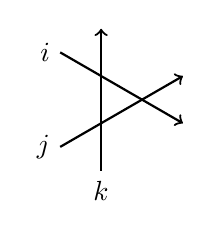
\begin{tikzpicture}[scale=0.6, baseline=(x.base)]
        \node (x) at (30:2) {};

        \draw[thick, ->] (0,0) node[left] {$j$} -- ++(30:3);
        \draw[thick, ->] (0,2) node[left] {$i$} -- ++(-30:3);
        \draw[thick, ->] (-30:1) node[below] {$k$} -- ++(0,3);

    \end{tikzpicture}
  \ =
    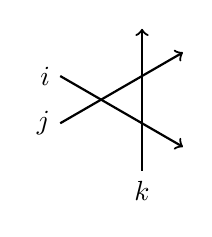
\begin{tikzpicture}[scale=0.6, baseline=(x.base)]
        \node (x) at (30:1) {};

        \draw[thick, ->] (0,0) node[left] {$j$} -- ++(30:3);
        \draw[thick, ->] (0,1) node[left] {$i$} -- ++(-30:3);
        \draw[thick, ->] (-30:2) node[below] {$k$} -- ++(0,3);

    \end{tikzpicture}
    \quad ,
\label{eq:intro_ybe0}
\end{equation}
where three intersecting lines are called \emph{rapidity lines} in the literature.
Each rapidity line carries a set of a vector space $V$ and a spectral parameter $u$
taking values in a Riemann surface.
At each crossing of the two lines, say $i$ and $j$, we associate an \emph{R-matrix}:
\begin{equation}
    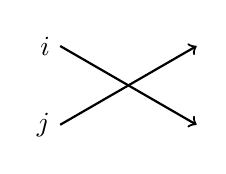
\begin{tikzpicture}[scale=1, baseline=(x.base)]  \node (x) at (0,0) {\vphantom{x}};

        \draw[thick, ->] (0,-0.5) node[left] {$j$} -- ++(30:2);
        \draw[thick, ->] (0,0.5) node[left] {$i$} -- ++(-30:2);

    \end{tikzpicture}
    \ =: \
    R_{ij}(u_i,u_j) \in \End(V_i\otimes V_j).
\end{equation}
Then, the Yang-Baxter equation reads
\begin{equation}
    R_{ij}(u_{i},u_{j})R_{ik}(u_{i},u_{k})R_{jk}(u_{j},u_{k})
        =  R_{jk}(u_{j},u_{k})R_{ik}(u_{i},u_{k})R_{ij}(u_{i},u_{j})
        ,
    \label{eq:intro_ybe}
\end{equation}
where each R-matrix is extended to an operator
$R_{ij}:=R_{ij}\otimes {\rm id}_{V_k}\in\End(V_i\otimes V_j\otimes V_k)$, etc.
R-matrix satisfying the Yang-Baxter equation implies a global relation,
that is, the transfer matrices constructed from the R-matrices commute each other.
When we have commuting transfer matrices, by expanding them with respect to the spectral parameters,
we obtain an infinite number of commuting conserved charges, that is another
definition of integrability.


Once we have the Yang-Baxter equation, we solve it and the solution yields an
integrable model.
This is, however, highly nontrivial.
For example, if one naively tries to solve the Yang-Baxter equation \eqref{eq:intro_ybe},
one finds that these equations are over-constrained in general.
To see this, let all the vector spaces $V_i$ be $N$-dimensional for simplicity.
Then the R-matrix associated with each crossing has four boundary lines and hence
has $O(N^4)$ components.
On the other hand, the Yang-Baxter equation, associated with diagrams with six boundary lines,
has $O(N^6)$ equations.
Even if one considers the simplest nontrivial case, $N=2$, the R-matrix has $16$ components
while they are constrained by $64$ equations.
The larger $N$ becomes, the severer this over-counting problem gets.
Thus, at first sight it seems hopeless that we could have a solution to the Yang-Baxter equation
\eqref{eq:intro_ybe},
but we know there exist solutions as well.


Now we arrive at the question: why integrable model exists?
If we have a good understanding of this question, then we can try to understand existing
integrable models from a unified perspective.
Furthermore, we may try to find new integrable models based on such understanding.
%
Indeed, there are two approaches to this question, both based on the ideas from quantum
field theory.
%For both approaches, the key concept is that there is a topological quantum field theory
%equipped with line operators localized in an extra dimensions.
%Actually,
These two approaches can also provide an answer to the first question given above.
Let us introduce them in order.


The first approach is based on four-dimensional analogue of Chern-Simons theory,
which is a cousin of the usual three-dimensional Chern-Simons theory but somewhat exotic.
The four-dimensional Chern-Simons theory can be defined only on a product manifold of a two-dimensional plane
and a Riemann surface, and the theory is partially topological and partially holomorphic on each two-manifold.
%they showed that the line operators extending
This theory was pioneered by Costello \cite{Costello:2013zra,Costello:2013sla},
and further investigated in \cite{Witten:2016spx,Costello:2017dso,Costello:2018gyb,Costello:2019tri}.
The ordinary three-dimensional Chern-Simons theory produces
quantum invariants of knots, links, and three-manifolds \cite{Witten:1988hf}.
It is well known that knots and links are closely related to integrable systems
(see e.g.~\cite{Wadati:1989ud} and the references therein),
but a direct connection between Chern-Simons theory and integrable systems was missing.
Costello, Witten and Yamazaki showed that in four-dimensional Chern-Simons theory, line operators
extending the topological plane generate a lattice model, and it is really an integrable lattice model.
An important fact here is that the line operators can be elongated only in the topological plane,
and their coordinates localized at the Riemann surface play the role of spectral parameters.
Therefore, what they demonstrated is that an integrable lattice model comes from line operators in a topological
quantum field theory with extra dimensions.


Another approach is based on supersymmetric quiver gauge theories, which is our main focus in this thesis.
Today this approach is called \emph{Gauge/YBE correspondence} \cite{Yamazaki:2012cp,Terashima:2012cx}.
This correspondence claims a more direct relation between the partition function, or supersymmetric index,
of quiver gauge theories and the partition function of integrable lattice models.
In fact, in this correspondence there is one-by-one mapping
between quiver gauge theories and integrable lattice models,
such as an identification between the quiver diagram and the lattice of an integrable spin system;
see figure \ref{fig:intro_gauge_ybe}.%
%
\footnote{More specifically, the index for vector and chiral multiplets
in quiver gauge theories are identified with the Boltzmann weights for
self- and nearest-neighbor interaction of spin systems, respectively.
We will show an explicit dictionary in section \ref{sec:tiling_latticemodel} of the main text.}
%
%
%FIGURE
\begin{figure}
    \centering
      \subfloat[\label{}]{
        \begin{tikzpicture}[scale=0.8, baseline=(x.base)]  \node (x) at (0,0) {\vphantom{x}};
          \def\site{1.2cm}

          \node[gnode] (a1) at (0,0) {};\node[gnode] (a2) at (\site,0) {};\node[gnode] (a3) at (2*\site,0) {};\node[gnode] (a4) at (3*\site,0) {};
          \begin{scope}[yshift=\site]
          \node[gnode] (b1) at (0,0) {};\node[gnode] (b2) at (\site,0) {};\node[gnode] (b3) at (2*\site,0) {};\node[gnode] (b4) at (3*\site,0) {};
          \end{scope}
          \begin{scope}[yshift=2*\site]
          \node[gnode] (c1) at (0,0) {};\node[gnode] (c2) at (\site,0) {};\node[gnode] (c3) at (2*\site,0) {};\node[gnode] (c4) at (3*\site,0) {};
          \end{scope}

          \draw[semithick, arrows=-latex] (a1) to (a2);\draw[semithick, arrows=-latex] (a3) to (a2);\draw[semithick, arrows=-latex] (a3) to (a4);
          \draw[semithick, arrows=-latex] (b2) to (b1);\draw[semithick, arrows=-latex] (b2) to (b3);\draw[semithick, arrows=-latex] (b4) to (b3);
          \draw[semithick, arrows=-latex] (c1) to (c2);\draw[semithick, arrows=-latex] (c3) to (c2);\draw[semithick, arrows=-latex] (c3) to (c4);

          \draw[semithick, arrows=-latex] (b1) to (a1);\draw[semithick, arrows=-latex] (a2) to (b2);
          \draw[semithick, arrows=-latex] (b3) to (a3);\draw[semithick, arrows=-latex] (a4) to (b4);
          \draw[semithick, arrows=-latex] (b1) to (c1);\draw[semithick, arrows=-latex] (c2) to (b2);
          \draw[semithick, arrows=-latex] (b3) to (c3);\draw[semithick, arrows=-latex] (c4) to (b4);

          \draw[semithick] (a1) to ++(-\site/2,0);\draw[semithick, arrows=latex-] (b1) to ++(-\site/2,0);\draw[semithick] (c1) to ++(-\site/2,0);
          \draw[semithick, arrows=latex-] (a4) to ++(\site/2,0); \draw[semithick] (b4) to ++(\site/2,0); \draw[semithick, arrows=latex-] (c4) to ++(\site/2,0);

          \draw[semithick, arrows=latex-] (a1) to ++(0,-\site/2);\draw[semithick] (a2) to ++(0,-\site/2);
          \draw[semithick, arrows=latex-] (a3) to ++(0,-\site/2);\draw[semithick] (a4) to ++(0,-\site/2);
          \draw[semithick, arrows=latex-] (c1) to ++(0,\site/2); \draw[semithick] (c2) to ++(0,\site/2);
          \draw[semithick, arrows=latex-] (c3) to ++(0,\site/2); \draw[semithick] (c4) to ++(0,\site/2);

        \end{tikzpicture}
        }
    \qquad\qquad
      \subfloat[\label{}]{
        \begin{tikzpicture}[scale=0.8, baseline=(x.base)]  \node (x) at (0,0) {\vphantom{x}};
          \def\site{1.2cm}

          \draw[semithick] (0,-\site/2) -- ++(0,3*\site);
          \draw[semithick, xshift=\site] (0,-\site/2) -- ++(0,3*\site);
          \draw[semithick, xshift=2*\site] (0,-\site/2) -- ++(0,3*\site);
          \draw[semithick, xshift=3*\site] (0,-\site/2) -- ++(0,3*\site);

          \draw[semithick] (-\site/2,0) -- ++(4*\site,0);
          \draw[semithick, yshift=\site] (-\site/2,0) -- ++(4*\site,0);
          \draw[semithick, yshift=2*\site] (-\site/2,0) -- ++(4*\site,0);

          \node[spin] (a1) at (0,0) {$s$};\node[spin] (a2) at (\site,0) {$s$};
          \node[spin] (a3) at (2*\site,0) {$s$};\node[spin] (a4) at (3*\site,0) {$s$};
          \begin{scope}[yshift=\site]
          \node[spin] (b1) at (0,0) {$s$};\node[spin] (b2) at (\site,0) {$s$};
          \node[spin] (b3) at (2*\site,0) {$s$};\node[spin] (b4) at (3*\site,0) {$s$};
          \end{scope}
          \begin{scope}[yshift=2*\site]
          \node[spin] (c1) at (0,0) {$s$};\node[spin] (c2) at (\site,0) {$s$};
          \node[spin] (c3) at (2*\site,0) {$s$};\node[spin] (c4) at (3*\site,0) {$s$};
          \end{scope}


        \end{tikzpicture}
        }
      \caption{In the Gauge/YBE correspondence, the quiver diagram specifying a
      gauge theory is identified with the lattice of an integrable spin system.}
      \label{fig:intro_gauge_ybe}
    \end{figure}
%
%
A topological structure behind the Gauge/YBE correspondence was elucidated in \cite{Yagi:2015lha}.
It is again a topological quantum field theory equipped with line operators
localized in extra dimensions.


Actually, four-dimensional Chern-Simons theory can eventually be
embedded into string theory setup \cite{Costello:2018txb} and
both approaches above are related to each other.
Based on these observations, we may conclude that the answer to the question
``why is there an integrable system behind supersymmetric gauge theory'' is
that we have a topological quantum field theory with line operators.
Moreover, this also answers to the question ``why does integrable system exist,''
since it is manifest that the Yang-Baxter equation \eqref{eq:intro_ybe0} is
satisfied by the topological nature of the system. %line operators in a topological quantum field theory
(Here notice that rapidity lines shown in \eqref{eq:intro_ybe0} are viewed as
line operators in a topological quantum field theory.)


The aim of this thesis is to give a unified picture of the above two approaches
using branes in string theory,
and present a more elaborate description of the correspondence between
supersymmetric gauge theories and integrable lattice models.
In doing so, we proceed to introducing further defect operators in
supersymmetric gauge theories. Then we study its counterpart in integrable
lattice model side.
The introduction of such additional defects enriches our correspondence,
and hopefully provide an insight into a new integrable system.
We will mostly work in the second approach, namely the correspondence between
quiver gauge theory and integrable lattice model.
%Both of our approach and that of four-dimensional Chern-Simons theory can eventually be
%embedded into string theory setup \cite{Costello:2018txb}.
%The both approaches are eventually embedded into string theory setup \cite{Costello:2018txb}.
We finally make comments on how our formulation of the correspondence is related to the setup of
four-dimensional Chern-Simons theory
%and clarify the relationship between the two
from the perspective of string dualities.
%four-dimensional Chern-Simons theory
%and our construction of the correspondences.







\subsection*{Organization of the thesis}


The structure of the thesis is shown as in figure \ref{fig:structure}.
Section \ref{sec:integrability} is devoted to a collection of basic facts regarding
topological quantum field theory, integrable lattice model, and
their realization by brane construction in string theory.
In section \ref{sec:preliminaries}, we briefly review the natural requirements for quantum field theory
and introduce Atiyah's axioms of topological quantum field theory (TQFT). Then we introduce lattice model as
a discrete version of quantum field theory in section \ref{sec:lattice_model}.
With these preparations, in section \ref{sec:integrability_from_TQFT}
we show that line operators in a topological quantum field theory and
integrable lattice models turn out to be equivalent through branes in string theory.
In section \ref{sec:surface}, we get into a concrete setup of the correspondence
between quiver gauge theories on spacetime $S^1\times S^3$ and
integrable lattice models of elliptic type.
There we add on additional surface defects in gauge theory side, and verify that they are
identified with the transfer matrix of the corresponding integrable lattice model.
In section \ref{sec:line}, we consider line defects in circular and linear quiver gauge
theories on $S^1\times \R^3$, which is based on the author's work \cite{Maruyoshi:2020cwy}.
Such line defects are represented as half-BPS Wilson-'t Hooft lines in gauge theories and
identified with transfer matrices of trigonometric type.
A variant of the AGT correspondence further implies an identification of the transfer matrices with
Verlinde line operators in Toda conformal field theory, which we also verify.
We clarify in section \ref{sec:branes} how these field theory setups are
related to four-dimensional Chern-Simons theory via embedding into string theory and dualities.
We conclude the thesis with some future directions in section \ref{sec:discussion}.


%FIGURE
\begin{figure}
    \centering
        %\subfloat[\label{}]{  }
        %\subfloat[\label{}]{  }
        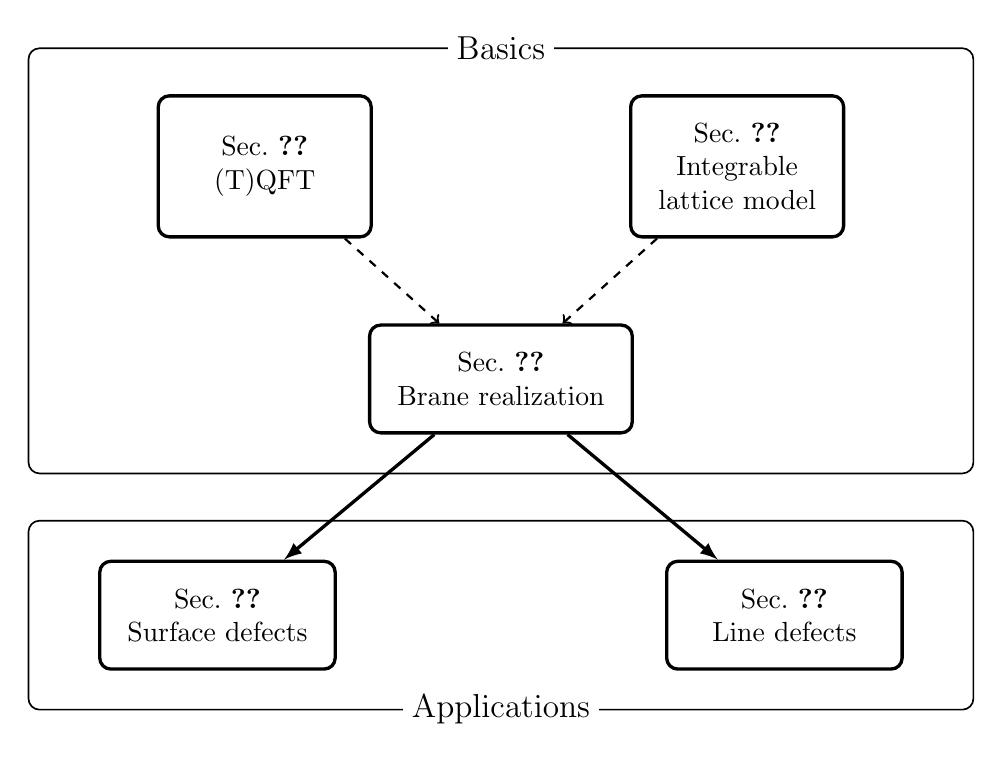
\begin{tikzpicture}[scale=1, baseline=(x.base), font=\normalsize]  \node (x) at (0,0) {\vphantom{x}};
            \def\sep{3cm}
            \tikzset{mysec/.style={rectangle,rounded corners,draw=black, %top color=white, bottom color=yellow!50,
                very thick, inner sep=1em, minimum size=3em, text centered}}

        \node[mysec, align=center] (B) at (0,0) {Sec.~\ref{sec:integrability_from_TQFT} \\ Brane realization};
        \node[mysec, align=center] (I) at (\sep,0.9*\sep) {Sec.~\ref{sec:lattice_model} \\ Integrable \\ lattice model};
        \node[mysec, align=center, text opacity=0] (T) at (-\sep,0.9*\sep) {Sec.~\ref{sec:lattice_model} \\ Integrable \\ lattice model};
        \node[align=center] at (-\sep,0.9*\sep) {Sec.~\ref{sec:preliminaries} \\ (T)QFT};

        \node[mysec, align=center] (S) at (-1.2*\sep,-1*\sep) {Sec.~\ref{sec:surface} \\ Surface defects};
        \node[mysec, align=center, text opacity=0] (L) at (1.2*\sep,-1*\sep) {Sec.~\ref{sec:line} \\ Surface defects};
        \node[align=center] at (1.2*\sep,-1*\sep) {Sec.~\ref{sec:line} \\ Line defects};

        \draw[thick, dashed, arrows=-to] (T) to (B);
        \draw[thick, dashed, arrows=-to] (I) to (B);
        \draw[very thick, arrows=-latex] (B) to (S);
        \draw[very thick, arrows=-latex] (B) to (L);


        \draw[semithick, rounded corners] (-2*\sep,-0.6*\sep) rectangle (2*\sep,-1.4*\sep);
        \draw[semithick, rounded corners] (-2*\sep,-0.4*\sep) rectangle (2*\sep,1.4*\sep);

        \node[fill=white, text centered, font=\large] at (0,1.4*\sep) {Basics};
        \node[fill=white, text centered, font=\large] at (0,-1.4*\sep) {Applications};


        \end{tikzpicture}
    \caption{Structure of the thesis.}
    \label{fig:structure}
\end{figure}



We also hope this thesis would be a good introductory review to the beautiful
and fascinating but largely unexplored connections among branes, topological
quantum field theories, and integrable systems.



%YBE can be seen as particle scattering and crossing of lattices













%%%%%%%%%%%%%%%%%%%%%%%%%%%%%%%%%%%%%%%%%%%%%%%%%%%%%%%%%



\bibliographystyle{Common/utphys}
%\nocite{*}
\bibliography{Common/Ref}



\end{document}
\documentclass[11pt, titlepage]{article}
%\ifnum 42146=\euc"A4A2 \AtBeginDvi{\special{pdf:tounicode EUC-UCS2}}\else %しおりが文字化けしないおまじない
%\AtBeginDvi{\special{pdf:tounicode 90ms-RKSJ-UCS2}}\fi %しおりが文字化けしないおまじない
\usepackage{amsmath,amssymb}
\usepackage{amsthm}
\usepackage{ascmac}
\usepackage{float}
%\usepackage[usenames]{color}
%\usepackage[dvips,usenames]{color}
\usepackage[pdftex]{graphicx}
%\usepackage[dvipdfmx]{graphicx}
\usepackage[color]{showkeys}
\usepackage[all]{xy}
\usepackage[pdftex,bookmarksnumbered=true,colorlinks=true,filecolor=blue,linkcolor=blue,urlcolor=blue,citecolor=red,linktocpage=true]{hyperref}
%\usepackage[dvipdfmx,bookmarksnumbered=true,colorlinks=true,filecolor=blue,linkcolor=blue,urlcolor=blue,citecolor=red,linktocpage=true]{hyperref}
%\usepackage[bookmarksnumbered=true,colorlinks=true,filecolor=blue,linkcolor=blue,urlcolor=blue,citecolor=red,linktocpage=true]{hyperref}

%\definecolor{labelkey}{rgb}{0.9451,0.2706,0.4941} %color for showkey
\definecolor{refkey}{rgb}{1,1,1} %color for showkey

\renewcommand{\baselinestretch}{1.3}

\setlength{\voffset}{-2cm}
\setlength{\oddsidemargin}{0.6cm}
\setlength{\evensidemargin}{0cm}
\setlength{\textwidth}{15.4cm}
\setlength{\textheight}{23cm}

\allowdisplaybreaks

\numberwithin{equation}{section}





%%%%%%%%%%%%%%%%%%%%%%%%%%%%%%%%%%%%%%%%%%%%%%%%%%

%\usepackage{jheppub}
\usepackage{upgreek}
\usepackage{slashed}
\usepackage{tikz}
\usepackage[caption=false,labelformat=simple]{subfig}
\renewcommand{\thesubfigure}{(\alph{subfigure})}




\usetikzlibrary{calc, positioning}
\usetikzlibrary{decorations.markings, arrows, bending}
\tikzset{
  font=\footnotesize,
  % Set arrowhead
  >=stealth,
  % Arrows with arrowhead in the middle
  ->-/.style={decoration={
      markings, mark=at position #1 with
      {\arrow{>}}},postaction={decorate}},
  -<-/.style={decoration={
      markings, mark=at position #1 with
      {\arrow{<}}},postaction={decorate}},
  % Spin site
  spin/.style={draw, fill=white, shape=circle, minimum size=11pt, inner
    sep=0pt, font=\scriptsize},
  % General node
  node/.style={draw, fill=white, shape=circle, minimum size=11pt, inner
    sep=0pt},
  % Gauge node
  gnode/.style={node},
  % Flavor node
  fnode/.style={node, shape=rectangle},
  % Theory node
  tnode/.style={fnode, double, minimum size=12pt},
  % Arrows
  q-/.style={-},
  q->/.style={->, shorten >=1pt, font=\smaller[2]},
  q<-/.style={q->, <-, shorten >=0pt, shorten <=1pt},
  % Equating flavor nodes
  eq-/.style={double, double distance=2pt},
}





\let\U\relax
\let\C\relax

\newcommand{\gf}{\mathfrak{g}}
\newcommand{\gfh}{\widehat{\gf}}
\newcommand{\hf}{\mathfrak{h}}
\newcommand{\sufh}{\widehat{\suf}}
\newcommand{\tf}{\mathfrak{t}}
\newcommand{\lf}{\mathfrak{l}}
\newcommand{\mf}{\mathfrak{m}}

\newcommand{\del}{\partial}
\newcommand{\delb}{{\bar\partial}}
\newcommand{\Ds}{\slashed{D}}
\newcommand{\dels}{\slashed{\del}}
\newcommand{\ind}{\mathop{\mathrm{index}}}
\newcommand{\id}{\mathop{\mathrm{id}}\nolimits}
\newcommand{\sgn}{\mathop{\mathrm{sgn}}\nolimits}

\newcommand{\vol}{\mathrm{vol}}
\def\ie{\begin{equation}\begin{aligned}}
\def\fe{\end{aligned}\end{equation}}
\newcommand{\set}[1]{\{#1\}}
\newcommand{\ket}[1]{|#1\rangle}
\newcommand{\bra}[1]{\langle #1|}
\newcommand{\Bigket}[1]{\Bigl|#1\Bigr\rangle}
\newcommand{\Bigbra}[1]{\Bigl\langle #1\Bigr|}
\newcommand{\abs}[1]{\lvert #1 \rvert}
\newcommand{\bigabs}[1]{\bigl\lvert #1 \bigr\rvert}
\newcommand{\Bigabs}[1]{\Bigl\lvert #1 \Bigr\rvert}
\newcommand{\biggabs}[1]{\biggl\lvert #1 \biggr\rvert}
\newcommand{\Biggabs}[1]{\Biggl\lvert #1 \Biggr\rvert}
\newcommand{\fixme}[1]{{\bf {\color{red}[#1]}}} 

\newcommand{\vev}[1]{\langle #1 \rangle}
\newcommand{\bigvev}[1]{\bigl\langle #1 \bigr\rangle}
\newcommand{\Bigvev}[1]{\Bigl\langle #1 \Bigr\rangle}
\newcommand{\biggvev}[1]{\biggl\langle #1 \biggr\rangle}
\newcommand{\Biggvev}[1]{\Biggl\langle #1 \Biggr\rangle}

\newcommand{\diag}{\mathop{\mathrm{diag}}\nolimits}
\newcommand{\Hom}{\mathop{\mathrm{Hom}}\nolimits}
\newcommand{\Map}{\mathop{\mathrm{Map}}\nolimits}
\newcommand{\ad}{\mathop{\mathrm{ad}}\nolimits}
\newcommand{\Ad}{\mathop{\mathrm{Ad}}\nolimits}
\newcommand{\ch}{\mathop{\mathrm{ch}}\nolimits}
\newcommand{\ich}{\mathit{ch}}
\newcommand{\rank}{\mathop{\mathrm{rank}}\nolimits}
\renewcommand{\Im}{\mathop{\mathrm{Im}}\nolimits}
\renewcommand{\Re}{\mathop{\mathrm{Re}}\nolimits}
\newcommand{\Ric}{\mathop{\mathrm{Ric}}\nolimits}
\newcommand{\Sym}{\mathop{\mathrm{Sym}}\nolimits}
\newcommand{\Tr}{\mathop{\mathrm{Tr}}\nolimits}
\newcommand{\End}{\mathop{\mathrm{End}}\nolimits}
\newcommand{\Res}{\mathop{\mathrm{Res}}\nolimits}
\renewcommand{\deg}{\mathop{\mathrm{deg}}\nolimits}
%\renewcommand{\span}{\mathop{\mathrm{span}}\nolimits}
\newcommand{\Lie}{\mathop{\mathrm{Lie}}\nolimits}
\newcommand{\qdet}{\mathop{\mathrm{qdet}}}
\newcommand{\crit}{\mathop{\mathrm{Crit}}}



\newcommand{\Hess}{\mathrm{Hess}}

\newcommand{\SU}{\mathrm{SU}}
\newcommand{\PSU}{\mathrm{PSU}}
\newcommand{\SO}{\mathrm{SO}}
\newcommand{\OO}{\mathrm{O}}
\newcommand{\Spin}{\mathrm{Spin}}
\newcommand{\Sp}{\mathrm{Sp}}
\newcommand{\SL}{\mathrm{SL}}
\newcommand{\GL}{\mathrm{GL}}
\newcommand{\glf}{\mathfrak{gl}}
\newcommand{\slf}{\mathfrak{sl}}
\newcommand{\suf}{\mathfrak{su}}
\newcommand{\sof}{\mathfrak{so}}
\newcommand{\PGL}{\mathrm{PGL}}
\newcommand{\PSL}{\mathrm{PSL}}
\newcommand{\U}{\mathrm{U}}

\newcommand{\Bun}{\mathrm{Bun}}
\newcommand{\Gr}{\mathrm{Gr}}

\newcommand{\iso}{\cong}

% Blackboard fonts
%\newcommand{\M}{\mathbb{M}}
\newcommand{\N}{\mathbb{N}}
\newcommand{\Z}{\mathbb{Z}}
\newcommand{\Q}{\mathbb{Q}}
\newcommand{\R}{\mathbb{R}}
\newcommand{\C}{\mathbb{C}}
\renewcommand{\H}{\mathbb{H}}
\renewcommand{\P}{\mathbb{P}}
\newcommand{\T}{\mathbb{T}}
%\renewcommand{\L}{\mathbb{L}}


% ALPHABETS

\let\nc\newcommand
\let\renc\renewcommand
\nc{\wbar}{\overline}
\let\td\tilde
\let\wtd\widetilde
\let\wht\widehat
\let\mcl\mathcal

\nc{\ab}{{\bar{a}}} \nc{\at}{\tilde{a}} \nc{\ah}{\hat{a}}
\nc{\bb}{{\bar{b}}} \nc{\bt}{\tilde{b}} \nc{\bh}{\hat{b}}
\nc{\cb}{{\bar{c}}} \nc{\ct}{\tilde{c}} %\nc{\ch}{\hat{c}}
\nc{\db}{{\bar{d}}} \nc{\dt}{\tilde{d}} \renc{\dh}{\hat{d}}
\nc{\eb}{{\bar{e}}} \nc{\et}{\tilde{e}} \nc{\eh}{\hat{e}}
\nc{\fb}{{\bar{f}}} \nc{\ft}{\tilde{f}} \nc{\fh}{\hat{f}}
\nc{\gb}{{\bar{g}}} \nc{\gt}{\tilde{g}} \nc{\gh}{\hat{g}}
\nc{\hb}{{\bar{h}}} \nc{\hh}{\hat{h}} %\nc{\ht}{\tilde{h}}
\nc{\ib}{{\bar{\imath}}} \nc{\ih}{\hat{\imath}} %\nc{\it}{\tilde{\imath}}
\nc{\jb}{{\bar{\jmath}}} \nc{\jt}{\tilde{\jmath}} \nc{\jh}{\hat{\jmath}}
\nc{\kb}{{\bar{k}}} \nc{\kt}{\tilde{k}} \nc{\kh}{\hat{k}}
\nc{\lb}{{\bar{l}}} \nc{\lt}{\tilde{l}} \nc{\lh}{\hat{l}}
\nc{\mb}{{\bar{m}}} \nc{\mt}{\tilde{m}} \nc{\mh}{\hat{m}}
\nc{\nb}{{\bar{n}}} \nc{\nt}{\tilde{n}} \nc{\nh}{\hat{n}}
\nc{\ob}{{\bar{o}}} \nc{\ot}{\tilde{o}} \nc{\oh}{\hat{o}}
\nc{\pb}{{\bar{p}}} \nc{\pt}{\tilde{p}} \nc{\ph}{\hat{p}}
\nc{\qb}{{\bar{q}}} \nc{\qt}{\tilde{q}} \nc{\qh}{\hat{q}}
\nc{\rb}{{\bar{r}}} \nc{\rt}{\tilde{r}} \nc{\rh}{{\hat{r}}}
\renc{\sb}{{\bar{s}}} \nc{\st}{\tilde{s}} \nc{\sh}{\hat{s}}
\nc{\tb}{{\bar{t}}} \renc{\th}{\hat{t}} %\nc{\tt}{\tilde{t}}
\nc{\ub}{{\bar{u}}} \nc{\ut}{\tilde{u}} \nc{\uh}{\hat{u}}
\nc{\vb}{{\bar{v}}} \nc{\vt}{\tilde{v}} \nc{\vh}{\hat{v}}
\nc{\wb}{{\bar{w}}} \nc{\wt}{\tilde{w}} \nc{\wh}{\hat{w}}
\nc{\xb}{{\bar{x}}} \nc{\xt}{\tilde{x}} \nc{\xh}{\hat{x}}
\nc{\yb}{{\bar{y}}} \nc{\yt}{\tilde{y}} \nc{\yh}{\hat{y}}
\nc{\zb}{{\bar{z}}} \nc{\zt}{\tilde{z}} \nc{\zh}{\hat{z}}

\nc{\Ab}{{\wbar{A}}} \nc{\At}{{\wtd{A}}} \nc{\Ah}{{\wht{A}}}
\nc{\Bb}{{\wbar{B}}} \nc{\Bt}{{\wtd{B}}} \nc{\Bh}{{\wht{B}}}
\nc{\Cb}{{\wbar{C}}} \nc{\Ct}{{\wtd{C}}} \nc{\Ch}{{\wht{C}}}
\nc{\Db}{{\wbar{D}}} \nc{\Dt}{{\wtd{D}}} \nc{\Dh}{{\wht{D}}}
\nc{\Eb}{{\wbar{E}}} \nc{\Et}{{\wtd{E}}} \nc{\Eh}{{\wht{E}}}
\nc{\Fb}{{\wbar{F}}} \nc{\Ft}{{\wtd{F}}} \nc{\Fh}{{\wht{F}}}
\nc{\Gb}{{\wbar{G}}} \nc{\Gt}{{\wtd{G}}} \nc{\Gh}{{\wht{G}}}
\nc{\Hb}{{\wbar{H}}} \nc{\Ht}{{\wtd{H}}} \nc{\Hh}{{\wht{H}}}
\nc{\Ib}{{\bar{I}}} \nc{\It}{{\wtd{I}}} \nc{\Ih}{{\wht{I}}}
\nc{\Jb}{{\wbar{J}}} \nc{\Jt}{{\wtd{J}}} \nc{\Jh}{{\wht{J}}}
\nc{\Kb}{{\wbar{K}}} \nc{\Kt}{{\wtd{K}}} \nc{\Kh}{{\wht{K}}}
\nc{\Lb}{{\wbar{L}}} \nc{\Lt}{{\wtd{L}}} \nc{\Lh}{{\wht{L}}}
\nc{\Mb}{{\wbar{M}}} \nc{\Mt}{{\wtd{M}}} \nc{\Mh}{{\wht{M}}}
\nc{\Nb}{{\wbar{N}}} \nc{\Nt}{{\wtd{N}}} \nc{\Nh}{{\wht{N}}}
\nc{\Ob}{{\wbar{O}}} \nc{\Ot}{{\wtd{O}}} \nc{\Oh}{{\wht{O}}}
\nc{\Pb}{{\wbar{P}}} \nc{\Pt}{{\wtd{P}}} \nc{\Ph}{{\wht{P}}}
\nc{\Qb}{{\wbar{Q}}} \nc{\Qt}{{\wtd{Q}}} \nc{\Qh}{{\wht{Q}}}
\nc{\Rb}{{\wbar{R}}} \nc{\Rt}{{\wtd{R}}} \nc{\Rh}{{\wht{R}}}
\nc{\Sb}{{\wbar{S}}} \nc{\St}{{\wtd{S}}} \nc{\Sh}{{\wht{S}}}
\nc{\Tb}{{\wbar{T}}} \nc{\Tt}{{\wtd{T}}} \nc{\Th}{{\wht{T}}}
\nc{\Ub}{{\wbar{U}}} \nc{\Ut}{{\wtd{U}}} \nc{\Uh}{{\wht{U}}}
\nc{\Vb}{{\wbar{V}}} \nc{\Vt}{{\wtd{V}}} \nc{\Vh}{{\wht{V}}}
\nc{\Wb}{{\wbar{W}}} \nc{\Wt}{{\wtd{W}}} \nc{\Wh}{{\wht{W}}}
\nc{\Xb}{{\wbar{X}}} \nc{\Xt}{{\wtd{X}}} \nc{\Xh}{{\wht{X}}}
\nc{\Yb}{{\wbar{Y}}} \nc{\Yt}{{\wtd{Y}}} \nc{\Yh}{{\wht{Y}}}
\nc{\Zb}{{\wbar{Z}}} \nc{\Zt}{{\wtd{Z}}} \nc{\Zh}{{\wht{Z}}}

\nc{\CA}{{\mcl{A}}} \nc{\CAb}{{\wbar{\CA}}} \nc{\CAt}{{\wtd{\CA}}} \nc{\CAh}{{\wht{\CA}}}
\nc{\CB}{{\mcl{B}}} \nc{\CBb}{{\wbar{\CB}}} \nc{\CBt}{{\wtd{\CB}}} \nc{\CBh}{{\wht{\CB}}}
\nc{\CC}{{\mcl{C}}} \nc{\CCb}{{\wbar{\CC}}} \nc{\CCt}{{\wtd{\CC}}} \nc{\CCh}{{\wht{\CC}}}
\nc{\cD}{{\mcl{D}}} \nc{\cDb}{{\wbar{\cD}}} \nc{\cDt}{{\wtd{\cC}}} \nc{\cDh}{{\wht{\cD}}}
\nc{\CE}{{\mcl{E}}} \nc{\CEb}{{\wbar{\CE}}} \nc{\CEt}{{\wtd{\CE}}} \nc{\CEh}{{\wht{\CE}}}
\nc{\CF}{{\mcl{F}}} \nc{\CFb}{{\wbar{\CF}}} \nc{\CFt}{{\wtd{\CF}}} \nc{\CFh}{{\wht{\CF}}}
\nc{\CG}{{\mcl{G}}} \nc{\CGb}{{\wbar{\CG}}} \nc{\CGt}{{\wtd{\CG}}} \nc{\CGh}{{\wht{\CG}}}
\nc{\CH}{{\mcl{H}}} \nc{\CHb}{{\wbar{\CH}}} \nc{\CHt}{{\wtd{\CH}}} \nc{\CHh}{{\wht{\CH}}}
\nc{\CI}{{\mcl{I}}} \nc{\CIb}{{\wbar{\CI}}} \nc{\CIt}{{\wtd{\CI}}} \nc{\CIh}{{\wht{\CI}}}
\nc{\CJ}{{\mcl{J}}} \nc{\CJb}{{\wbar{\CJ}}} \nc{\CJt}{{\wtd{\CJ}}} \nc{\CJh}{{\wht{\CJ}}}
\nc{\CK}{{\mcl{K}}} \nc{\CKb}{{\wbar{\CK}}} \nc{\CKt}{{\wtd{\CK}}} \nc{\CKh}{{\wht{\CK}}}
\nc{\CL}{{\mcl{L}}} \nc{\CLb}{{\wbar{\CL}}} \nc{\CLt}{{\wtd{\CL}}} \nc{\CLh}{{\wht{\CL}}}
\nc{\CM}{{\mcl{M}}} \nc{\CMb}{{\wbar{\CM}}} \nc{\CMt}{{\wtd{\CM}}} \nc{\CMh}{{\wht{\CM}}}
\nc{\CN}{{\mcl{N}}} \nc{\CNb}{{\wbar{\CN}}} \nc{\CNt}{{\wtd{\CN}}} \nc{\CNh}{{\wht{\CN}}}
\nc{\CO}{{\mcl{O}}} \nc{\COb}{{\wbar{\CO}}} \nc{\COt}{{\wtd{\CO}}} \nc{\COh}{{\wht{\CO}}}
\nc{\CP}{{\mcl{P}}} \nc{\CPb}{{\wbar{\CP}}} \nc{\CPt}{{\wtd{\CP}}} \nc{\CPh}{{\wht{\CP}}}
\nc{\CQ}{{\mcl{Q}}} \nc{\CQb}{{\wbar{\CQ}}} \nc{\CQt}{{\wtd{\CQ}}} \nc{\CQh}{{\wht{\CQ}}}
\nc{\CR}{{\mcl{R}}} \nc{\CRb}{{\wbar{\CR}}} \nc{\CRt}{{\wtd{\CR}}} \nc{\CRh}{{\wht{\CR}}}
\nc{\CS}{{\mcl{S}}} \nc{\CSb}{{\wbar{\CS}}} \nc{\CSt}{{\wtd{\CS}}} \nc{\CSh}{{\wht{\CS}}}
\nc{\CT}{{\mcl{T}}} \nc{\CTb}{{\wbar{\CT}}} \nc{\CTt}{{\wtd{\CT}}} \nc{\CTh}{{\wht{\CT}}}
\nc{\CU}{{\mcl{U}}} \nc{\CUb}{{\wbar{\CU}}} \nc{\CUt}{{\wtd{\CU}}} \nc{\CUh}{{\wht{\CU}}}
\nc{\CV}{{\mcl{V}}} \nc{\CVb}{{\wbar{\CV}}} \nc{\CVt}{{\wtd{\CV}}} \nc{\CVh}{{\wht{\CV}}}
\nc{\CW}{{\mcl{W}}} \nc{\CWb}{{\wbar{\CW}}} \nc{\CWt}{{\wtd{\CW}}} \nc{\CWh}{{\wht{\CW}}}
\nc{\CX}{{\mcl{X}}} \nc{\CXb}{{\wbar{\CX}}} \nc{\CXt}{{\wtd{\CX}}} \nc{\CXh}{{\wht{\CX}}}
\nc{\CY}{{\mcl{Y}}} \nc{\CYb}{{\wbar{\CY}}} \nc{\CYt}{{\wtd{\CY}}} \nc{\CYh}{{\wht{\CY}}}
\nc{\CZ}{{\mcl{Z}}} \nc{\CZb}{{\wbar{\CZ}}} \nc{\CZt}{{\wtd{\CZ}}} \nc{\CZh}{{\wht{\CZ}}}

\let\eps\epsilon
\let\ups\upsilon
\let\veps\varepsilon
\let\vtht\vartheta
\let\vtheta\vtht
\let\vsgm\varsigma
\let\vphi\varphi
\let\vrho\varrho

\nc{\alphab}{{\bar{\alpha}}} \nc{\alphat}{{\td{\alpha}}} \nc{\alphah}{{\hat{\alpha}}}
\nc{\betab}{{\bar{\beta}}}   \nc{\betat}{{\td{\beta}}}   \nc{\betah}{{\hat{\beta}}} 
\nc{\gammab}{{\bar{\gamma}}} \nc{\gammat}{{\td{\gamma}}} \nc{\gammah}{{\hat{\gamma}}} 
\nc{\deltab}{{\bar{\delta}}} \nc{\deltat}{{\td{\delta}}} \nc{\deltah}{{\hat{\delta}}} 
\nc{\epsilonb}{{\bar{\eps}}} \nc{\epsilont}{{\td{\eps}}} \nc{\epsilonh}{{\hat{\eps}}} 
\nc{\vepsb}{{\bar{\veps}}}   \nc{\vepst}{{\td{\veps}}}   \nc{\vepsh}{{\hat{\veps}}} 
\nc{\zetab}{{\bar{\zeta}}}   \nc{\zetat}{{\td{\zeta}}}   \nc{\zetah}{{\hat{\zeta}}} 
\nc{\etab}{{\bar{\eta}}}     \nc{\etat}{{\td{\eta}}}     \nc{\etah}{{\hat{\eta}}} 
\nc{\thetab}{{\bar{\theta}}} \nc{\thetat}{{\td{\theta}}} \nc{\thetah}{{\hat{\theta}}} 
\nc{\vthetab}{{\bar{\vtht}}} \nc{\vthetat}{{\td{\vtht}}} \nc{\vthetah}{{\hat{\vtht}}} 
\nc{\lambdab}{{\bar{\lambda}}} \nc{\lambdat}{{\td{\lambda}}} \nc{\lambdah}{{\hat{\lambda}}} 
\nc{\iotab}{{\bar{\iota}}}   \nc{\iotat}{{\td{\iota}}}   \nc{\iotah}{{\hat{\iota}}} 
\nc{\kappab}{{\bar{\kappa}}} \nc{\kappat}{{\td{\kappa}}} \nc{\kappah}{{\hat{\kappa}}} 
\nc{\lmdb}{{\bar{\lmd}}}     \nc{\lmdt}{{\td{\lmd}}}     \nc{\lmdh}{{\hat{\lmd}}} 
\nc{\mub}{{\bar{\mu}}}       \nc{\mut}{{\td{\mu}}}       \nc{\muh}{{\hat{\mu}}} 
\nc{\nub}{{\bar{\nu}}}       \nc{\nut}{{\td{\nu}}}       \nc{\nuh}{{\hat{\nu}}} 
\nc{\xib}{{\bar{\xi}}}       \nc{\xit}{{\td{\xi}}}       \nc{\xih}{{\hat{\xi}}} 
\nc{\pib}{{\bar{\pi}}}       \nc{\pit}{{\td{\pi}}}       \nc{\pih}{{\hat{\pi}}} 
\nc{\vpib}{{\bar{\vpi}}}     \nc{\vpit}{{\td{\vpi}}}     \nc{\vpih}{{\hat{\vpi}}} 
\nc{\rhob}{{\bar{\rho}}}     \nc{\rhot}{{\td{\rho}}}     \nc{\rhoh}{{\hat{\rho}}} 
\nc{\vrhob}{{\bar{\vrho}}}   \nc{\vrhot}{{\td{\vrho}}}   \nc{\vrhoh}{{\hat{\vrho}}} 
\nc{\sigmab}{{\bar{\sigma}}} \nc{\sigmat}{{\td{\sigma}}} \nc{\sigmah}{{\hat{\sigma}}} 
\nc{\vsigmab}{{\bar{\vsgm}}} \nc{\vsigmat}{{\td{\vsgm}}} \nc{\vsigmah}{{\hat{\vsgm}}} 
\nc{\taub}{{\bar{\tau}}}     \nc{\taut}{{\td{\tau}}}     \nc{\tauh}{{\hat{\tau}}} 
\nc{\upsb}{{\bar{\ups}}} \nc{\upst}{{\td{\ups}}} \nc{\upsh}{{\hat{\ups}}} 
\nc{\phib}{{\bar{\phi}}}     \nc{\phit}{{\td{\phi}}}     \nc{\phih}{{\hat{\phi}}} 
\nc{\varphib}{{\bar{\vphi}}}   \nc{\varphit}{{\td{\vphi}}}   \nc{\varphih}{{\hat{\vphi}}} 
\nc{\chib}{{\bar{\chi}}}     \nc{\chit}{{\td{\chi}}}     \nc{\chih}{{\hat{\chi}}} 
\nc{\psib}{{\bar{\psi}}}     \nc{\psit}{{\td{\psi}}}     \nc{\psih}{{\hat{\psi}}} 
\nc{\omegab}{{\bar{\omega}}} \nc{\omegat}{{\td{\omega}}} \nc{\omegah}{{\hat{\omega}}} 

\nc{\Gammab}{{\wbar{\Gamma}}}     \nc{\Gammat}{{\wtd{\Gamma}}}     \nc{\Gammah}{{\wht{\Gamma}}}
\nc{\Deltab}{{\wbar{\Delta}}}     \nc{\Deltat}{{\wtd{\Delta}}}     \nc{\Deltah}{{\wht{\Delta}}}
\nc{\Thetab}{{\wbar{\Theta}}}     \nc{\Thetat}{{\wtd{\Theta}}}     \nc{\Thetah}{{\wht{\Theta}}}
\nc{\Lambdab}{{\wbar{\Lambda}}}   \nc{\Lambdat}{{\wtd{\Lambda}}}   \nc{\Lambdah}{{\wht{\Lambda}}}
\nc{\Xib}{{\wbar{\Xi}}}           \nc{\Xit}{{\wtd{\Xi}}}           \nc{\Xih}{{\wht{\Xi}}}
\nc{\Pib}{{\wbar{\Pi}}}           \nc{\Pit}{{\wtd{\Pi}}}           \nc{\Pih}{{\wht{\Pi}}}
\nc{\Sigmab}{{\wbar{\Sigma}}}     \nc{\Sigmat}{{\wtd{\Sigma}}}     \nc{\Sigmah}{{\wht{\Sigma}}}
\nc{\Upsilonb}{{\wbar{\Upsilon}}} \nc{\Upsilont}{{\wtd{\Upsilon}}} \nc{\Upsilonh}{{\wht{\Upsilon}}}
\nc{\Phib}{{\wbar{\Phi}}} \nc{\Phit}{{\wtd{\Phi}}} \nc{\Phih}{{\wht{\Phi}}}
\nc{\Psib}{{\wbar{\Psi}}}         \nc{\Psit}{{\wtd{\Psi}}}         \nc{\Psih}{{\wht{\Psi}}}
\nc{\Omegab}{{\wbar{\Omega}}}     \nc{\Omegat}{{\wtd{\Omega}}}     \nc{\Omegah}{{\wht{\Omega}}}


\newcommand{\rmd}{\mathrm{d}}
\newcommand{\epsb}{\epsilonb}
\newcommand{\ChS}{\mathrm{CS}}

\newcommand{\auxP}{\mathsf{P}}
\newcommand{\auxF}{\mathsf{F}}
\newcommand{\auxFb}{\overline{\auxF}}
\newcommand{\auxD}{\mathsf{D}}
\newcommand{\auxB}{\mathsf{B}}
\newcommand{\phibt}{\tilde{\phib}}
\newcommand{\iu}{\mathrm{i}}
%\newcommand{\iu}{i}

\let\starx\star
\let\star\relax
\newcommand{\star}{\mathop{\starx}\nolimits}

\newcommand{\SV}{S_{\text{V}}}
\newcommand{\SC}{S_{\text{C}}}
\newcommand{\SW}{S_W}
\newcommand{\GF}{\text{GF}}
\newcommand{\SGF}{S_{\text{GF}}}
\newcommand{\BRST}{\text{BRST}}

%\newcommand{\sslash}{/\mkern-6mu/}

\newcommand{\mm}{\upmu} % Moment map


\newcommand{\V}{\mathbb{V}}

\newcommand{\RF}{R^{\text{F}}}
\newcommand{\LF}{L^{\text{F}}}
\newcommand{\LFt}{\Lt^{\text{F}}}
\newcommand{\RBS}{R^{\text{BSDS}}}
\newcommand{\LBS}{L^{\text{BS}}}
\newcommand{\RB}{R^{\text{B}}}
\newcommand{\RBt}{\Rt^{\text{B}}}
\newcommand{\RFt}{\Rt^{\text{F}}}
\newcommand{\RFb}{\Rb^{\text{F}}}
\newcommand{\RBSt}{\Rt^{\text{BS}}}
\newcommand{\RDS}{\RM^{\text{DS}}}
\newcommand{\hol}{\mathop{\mathrm{hol}}\nolimits}
\newcommand{\qs}{\mathsf{q}}

%\usepackage[mathscr]{euscript}

%\newcommand{\Spinor}{\mathscr{S}}
\newcommand{\Spinor}{S}
\newcommand{\PB}{P}
\newcommand{\KB}{\overline{K}}
\newcommand{\SG}{\mathscr{G}}
\newcommand{\SR}{\mathscr{R}}
\renewcommand{\SV}{\mathscr{V}}
\newcommand{\SP}{\mathscr{P}}
\newcommand{\ST}{\mathscr{T}}
\newcommand{\STb}{\overline{\mathscr{T}}}
\newcommand{\Mod}{\mathscr{M}}
\newcommand{\Lag}{\mathscr{L}}


\newcommand{\Qone}{\mathbf{Q}}
\newcommand{\QQ}{\slashed{Q}}
\newcommand{\QQt}{\widetilde{\QQ}}
\newcommand{\QK}{Q_K}
\newcommand{\QQK}{\QQ_{\mathrm{K}}}
\newcommand{\QQtK}{\QQt_{\mathrm{K}}}

\newcommand{\RW}{{\mathrm{RW}}}
\newcommand{\mRW}{{\mathrm{mRW}}}
\newcommand{\adj}{\mathrm{adj}}
\newcommand{\conf}{\mathrm{Conf}}

\newcommand{\betaSD}{\upbeta}
\newcommand{\gammaSD}{\upgamma}
\newcommand{\bSD}{\mathtt{b}}
\newcommand{\cSD}{\mathtt{c}}

\newcommand{\lbracket}[3]{\{#2 {}_{\,#1\,} #3\}}
\newcommand{\lBracket}[3]{[#2 {}_{\,#1\,} #3]}

\newcommand{\zmode}{{\textstyle\int}}

\newcommand{\NO}[1]{{\mathopen:\,#1\,\mathclose:}}
\newcommand{\ec}[1]{[\![#1]\!]}
\newcommand{\bigec}[1]{\bigl[\!\bigl[#1\bigr]\!\bigr]}
\newcommand{\biggec}[1]{\biggl[\!\!\biggl[#1\biggr]\!\!\biggr]}


\newcommand{\as}{\mathsf{a}}
\newcommand{\bs}{\mathsf{b}}
\newcommand{\ms}{\mathsf{m}}

\newcommand{\rootl}{\Lambda_{\mathrm{r}}}
\newcommand{\corootl}{\Lambda_{\mathrm{cr}}}
\newcommand{\weightl}{\Lambda_{\mathrm{w}}}
\newcommand{\coweightl}{\Lambda_{\mathrm{cw}}}

\newcommand{\mcharge}{\mathbf{m}}
\newcommand{\echarge}{\mathbf{e}}

%%%%%%%%%%%%%%%%%%%%%%%%%%%%%%%%%%%%%%%%%%%%%%%%%%






\begin{document}



%%%%%%%%%%%%%%%%%% section 2 %%%%%%%%%%%%%%%%%%%%%%%%%%%%%%%%%
\section{Integrability from extra dimensions}


Throughout this paper, we discuss correspondences between
a certain class of supersymmetric gauge theories and integrable lattice
models: 
\begin{equation}
 \mathcal{I}_{\mathsf{T}_{4d}\left[\mathsf{L}_{2d}\right]}
	=  Z_{\mathsf{L}_{2d}\left[\mathsf{T}_{4d}\right]},
\end{equation}
where the left-hand side is the supersymmetric index of a four-dimensional
gauge theory $\mathsf{T}_{4d}$ and the right-hand side denotes the
statistical partition function of the corresponding integrable lattice
model $\mathsf{L}_{2d}$ specified by the four-dimensional theory
$\mathsf{T}_{4d}$. As it turns out, the correspondence emerges from
TQFT with extra dimensions \cite{Yagi:2015lha}. The aim of this section is
to give the step-by-step explanation of the above correspondence from
an elementary level. Besides, to explain these, we will start by clarifying
in order what the terms TQFT, lattice model, and integrability mean. 





\subsection{Preliminaries}

In the next subsection, we would like to introduce lattice model as
discrete quantum field theory (QFT). So let us start from the general
settings of QFT. We first briefly review one-dimensional QFT, which
is nothing but quantum mechanics, and then extend the discussion to
general quantum field theory in ($d+1$)-dimensions. Though we do
not have a complete definition of general QFT, a special class of
QFT which is called \emph{topological} QFT is axiomatized by Atiyah
\cite{Atiyah:1989vu}. 





\subsubsection{What is quantum field theory?}

Let us now begin with one-dimensional QFT, as known as quantum mechanics
(QM). Suppose we have a one-dimensional manifold%
%
\footnote{Throughout the paper, we assume all the manifold is smooth and oriented,
unless otherwise stated. }%
%
, which may be thought of as ``time'' $M^{1}=$ interval or $S^{1}$
(or $\mathbb{R}$), and data to specify a QM: 
\begin{itemize}
 \item $\mathcal{H}$ : a vector space (Hilbert space/state space), 
 \item $\mathcal{O}$ : a set of self-adjoint operators (observables, acting
on $\mathcal{H}$),
 \item $H$ : an operator called \emph{Hamiltonian}, 
\end{itemize}
where $H\in\mathcal{O}$ and the state space $\mathcal{H}$ is a finite
or infinite dimensional $\mathbb{C}$-vector space. We sometimes need
to consider a set of operators $\mathcal{O}$ including not self-adjoint
operators, but for simplicity we do not care about that at this moment.
In undergraduate, we have learnt that one should consider the Schr\"{o}dinger
equation and find a good basis in $\mathcal{H}$ diagonalizing the
Hamiltonian. 

Formally, the procedure of solving the Schr\"{o}dinger equation leads
to an expression of time evolution of states by a linear map%
%
\footnote{We here do not get into the argument of Euclideanization.}
%
$e^{-tH}$ in quantum mechanics, and the partition function in many-body
statistical mechanics. In turn, we have two most crucial properties
of QM: Given an interval $M^{1}=\left[t_{0},t_{1}\right]$, we have
state vectors at the endpoints of the interval and a time evolution
between the states: 
\begin{equation}
    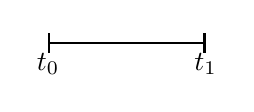
\begin{tikzpicture}[scale=1.0, baseline=(x.base)]    \node (x) at (0,0) {\vphantom{x}};
        
        \draw[thick, arrows=|-|] (0,0) node[below=0.1] {$t_0$} -- (2,0) node[below=0.1] {$t_1$};
        
    \end{tikzpicture}
  \quad \rightsquigarrow \quad
  e^{-\left(t_{1}-t_{0}\right)H} : \mathcal{H}  \longrightarrow  \mathcal{H} \, ,
\end{equation}
 and given a circle $M^{1}=S_{\beta}^{1}$, we get a number called
\emph{partition function}:
\begin{equation}
    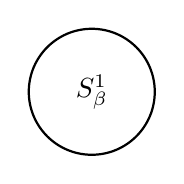
\begin{tikzpicture}[scale=0.8, baseline=(x.base)]    \node (x) at (0,0) {\vphantom{x}};
        
        \draw[thick] (0,0) circle[radius=1cm] node {$S^1_{\beta}$};
%        \draw[thick] (0.9,0) -- (1.1,0) node[right] {$t=0,\, \beta$};
%        \node at (0.5,1.5) {\large${\rm Tr}_{\mathcal{H}} e^{-\beta H}$};
        
    \end{tikzpicture}
  \quad \rightsquigarrow \quad
  \mathrm{Tr}_{\mathcal{H}}  e^{-\beta H} \, .
\end{equation}


%FIGURE
\begin{figure}
\centering
  \subfloat[\label{fig:qm_interval}]{
    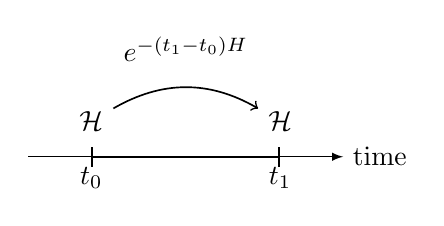
\begin{tikzpicture}[scale=1.0] %, baseline=(x.base)]    \node (x) at (0,0) {\vphantom{x}};
        
        \draw[arrows=-latex] (0,0) -- (4,0) node[right] {time};
        \draw[thick, arrows=|-|] (0.8,0) node[above=0.2cm] (H0) {\normalsize $\mathcal{H}$} node[below=0.1] {$t_0$} -- (3.2,0) node[above=0.2cm] (H1) {\normalsize $\mathcal{H}$} node[below=0.1] {$t_1$};
        \draw[semithick, arrows=-to] (H0) to[bend left=30] node[above=0.2cm, pos=0.5] {\normalsize $e^{-(t_1 - t_0)H}$} (H1);
        
    \end{tikzpicture}
  }
  \qquad\qquad
  \subfloat[\label{fig:qm_circle}]{
    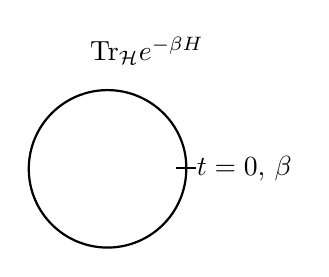
\begin{tikzpicture}[scale=1.0] %, baseline=(x.base)]    \node (x) at (0,0) {\vphantom{x}};
        
        \draw[thick, arrows=|-] (1,0) node[right=0.1] {$t=0,\, \beta$} arc (0:360:1);
        
%        \draw[thick] (0,0) circle[radius=1cm];
%        \draw[thick] (0.9,0) -- (1.1,0) node[right] {$t=0,\, \beta$};
        \node at (0.5,1.5) {\normalsize ${\rm Tr}_{\mathcal{H}} e^{-\beta H}$};
        
    \end{tikzpicture}
  }
  \caption{Two most crucial properties of quantum mechanics.}
  \label{fig:qm_two_properties}
\end{figure}


In addition, from the physical facts it is quite reasonable to assume
that the time evolution and the partition function are compatible
with cutting and gluing intervals and $S^{1}$s. This simply means
that the time evolution from time $t_{0}$ to $t_{1}$ followed by
another time evolution from $t_{1}$ to $t_{2}$ is equal to the single
time evolution from $t_{0}$ to $t_{2}$, etc. Summarizing, the properties
that quantum mechanics or one-dimensional QFT has are rephrased by
the language of given one-dimensional manifold $M^{1}$ (see figure \ref{fig:qm_two_properties}): 
\begin{itemize}
  \item Given an interval, produces state vectors at the endpoints and a linear
map between them. 
  \item Given an $S^{1}$, produces a number. 
  \item Compatible with cutting and gluing intervals and $S^{1}$s. 
\end{itemize}
Thus, in the abstract we conclude that one-dimensional QFT, or quantum
mechanics, is a gadget satisfying the above properties for each given
one-dimensional manifold $M^{1}$. 

From these observations of quantum mechanics, we wish to extend the
discussion to general ($d+1$)-dimensional QFT. The starting point
of defining a ($d+1$)-dimensional QFT is the choice of a ($d+1$)-dimensional
manifold $M^{d+1}$, which has $d$ spatial directions and one ``time''
direction. For most QFTs the manifold $M^{d+1}$ is viewed as a Riemannian
manifold with a smooth metric on it. As already noticed, we will mostly
consider a positive definite Riemannian metric, QFT on which is usually
referred to as an Euclidean QFT, and hence precisely there is no notion
of ``time'' in such a theory, at least globally. The manifold $M^{d+1}$
may or may not have boundaries. In case it does have boundaries some
additional information is needed at the boundaries to define the QFT.
In addition to a Riemannian metric, depending on the situation one
wants to consider, one often needs some more structures on the manifold
$M^{d+1}$, e.g. smooth structure, conformal structure, spin structure,
etc. 

To obtain the data to specify a QFT, we now would like to extend the
observations seen in QM. Suppose we have a ($d+1$)-dimensional manifold
$M^{d+1}$, then we wish to ``define'' a QFT by a gadget $Z$, which
should produce a vector when $M^{d+1}$ has a boundary 
\begin{equation}
Z\left(M^{d+1}\right)  \in  \mathcal{H}_{bdy},
\end{equation}
 and should produce a number when $M^{d+1}$ has no boundary 
\begin{equation}
Z\left(M^{d+1}\right)  \in  \mathbb{C}.
\end{equation}
 %
In the case of $M^{d+1}$ with a boundary, the vector space defined
on the boundary is called the space of states or just Hilbert space
in the physics literature. On the one hand, if $M^{d+1}$ does not
have boundary, the number $Z\left(M^{d+1}\right)$ is called the partition
function. If the boundary of $M^{d+1}$ has several disconnected components,
namely the boundaries are given by the disjoint union of simply connected
$d$-dimensional closed manifolds $\left\{ N_{i}^{d}\right\} $: $\partial M^{d+1}=\sqcup_{i}N_{i}^{d}$,
$Z$ should define a linear map among the vector spaces defined on
the boundaries. In particular, in the case $M^{d+1}=N^{d}\times I$,
where $I$ is an interval of length $T$, $M^{d+1}$ has two boundaries
$N^{d}$ and $Z$ now gives rise to a linear map $Z\left(N^{d}\times I\right)=:U\left(T\right)$,
\begin{equation}
  U\left(T\right)  :  \mathcal{H}_{N}  \longrightarrow  \mathcal{H}_{N}.
\end{equation}
From the physical facts, $Z$ also should be compatible with cutting and
gluing of ($d+1$)-dimensional manifolds, and thus we learn that the
linear map given above satisfies $U\left(T_{1}\right)U\left(T_{2}\right) = U\left(T_{1}+T_{2}\right)$.
This in turn defines an operator $H$ as the generator of $U$, 
\begin{equation}
  U\left(T\right)  =  \exp\left(-TH\right).
\end{equation}
 $H$ is called the Hamiltonian of the system, acting on the space
of states $\mathcal{H}_{N}$. If one considers a manifold
with Lorentzian metric, $U\left(T\right)$ is represented as 
\begin{equation}
  U\left(T\right)  =  \exp\left(-iTH\right),
\end{equation}
and then the interval $I$ is regarded as ``physical time.'' 

\subsubsection{Construction of $Z$}

So far we have discussed only in an abstract way what quantum field
theory is, or in other words what the gadget $Z$ should satisfy.
Let us now see how we specify $Z$ to define a QFT. Broadly speaking,
there are three kinds of constructions of $Z$. They are not totally
independent and have many aspects of applicabilities. In the rest
of this section, $M$ denotes a ($d+1$)-dimensional manifold with
or without boundary, and $N$ denotes a $d$-dimensional closed manifold
without boundary. 

\subsubsection*{Construct from the axiom}

The first construction is in a sense the simplest one; we write down
appropriate properties that a QFT must satisfy, and axiomatize them.
Construction of $Z$ is to give a mathematical formulation which satisfy
the axioms as the data to specify the theory. This is actually the
only way that one can define a QFT by mathematically rigorous procedures.
Normally, such a theory is first studied by physicists as an ideal
or a toy model from the physical motivation, and then refined as rigorous
mathematics by mathematicians.%
%
\footnote{The fact that a QFT can be treated in a mathematically rigorous way
implies that the theory may have an enormous amount of symmetry, and
the difficulties of the QFT are completely controlled by them. Even
better, these theories can often be exactly solved in an appropriate
sense.}
%
 There are several kinds of such theories. We now introduce typical
three examples. 

The first one is \emph{free theories} in any dimensions, which are
toy models of field theories and play important roles as a probe of
more complicated QFTs. In any spacetime dimensions, for the Riemannian
manifolds with or without spin structure, we can rigorously define
the free field theories. One of them is the free scalar field theory.
Besides a ($d+1$)-dimensional closed manifold $M$, pick a $G$-bundle
$P\rightarrow M$ with connection $A$ and a $G$-vector space $V$.
Then we construct the associated vector bundle $P\times_{G}V$, whose
covariant derivative is denoted by $D_{A}$. We now have the Laplacian
$\Delta_{A}$ given by the covariant derivative $D_{A}$, and then
the free scalar field theory is defined by the partition function
\begin{equation}
  Z_{\mathrm{scalar}}\left(M;A\right)  :=  1/\det\Delta_{A}.
\end{equation}
 If the determinant of the Laplacian involves a divergence, it must
be properly removed. 

Another free theory is the free fermion theory. In this case $M$
also needs a spin structure and the spin representations $S$, $S'$.
Then we construct the Dirac operator $\mathcal{D}_{A}$ on the spin
bundles and the partition function of the free fermion theory is given
by 
\begin{equation}
Z_{\mathrm{fermion}}\left(M;A\right):=\det\mathcal{D}_{A},
\end{equation}
 again the determinant is taken appropriately.%
%
\footnote{Fermion theories may have anomalies. If it is the case, the axiom
needs to be somehow modified. In particular the partition function
for a closed manifold is given by the eta invariant \cite{Dai:1994kq}. }

Next, in two dimensions, we have another axiomatic quantum field theory,
that is \emph{conformal field theory} (CFT). Conformal field theory
in two dimensions was originally formulated by Belavin, Polyakov,
and Zamolodchikov \cite{Belavin:1984vu} as a model of physical systems at critical
points. They established the renowned Virasoro algebra as an infinite
dimensional symmetry of the system and fully investigated the minimal
model. The holomorphic part of the Virasoro algebra is captured by
vertex operator algebras, and since then there are many mathematically
rigorous discussions on them. Their kinematic behaviors on Riemann
surfaces are governed by the conformal blocks, and its geometric meaning
has been studied in \cite{Friedan:1986ua}. In turn, the study of irrational
CFTs has led to the AGT correspondence \cite{Alday:2009aq}, which has brought
to us large amount of developments in both physics and mathematics. 

The final example is \emph{topological quantum field theories} (TQFTs).
TQFT is one of the main focuses in this paper. These theories are
originating from Witten's proposals of topological field theories
\cite{Witten:1988xj, Witten:1988ze, Witten:1988hf}. Inspired by Witten's
proposals, Atiyah and Segal axiomatized the topological QFT,%
%
\footnote{Precisely speaking, what Segal axiomatized is the definition of conformal
field theories \cite{Segal:2002ei}. However, at any rate the definition of CFT by Segal
is quite similar to the definition of Atiyah's TQFT, namely it is a
categorical one. For the geometric definition of CFT, see \cite{Friedan:1986ua}. }
%
 and happily this also has brought to us a numerous amount of applications
both to physics and to pure mathematics. For example, ($1+1$)-dimensional
topological QFTs are known to be categorically equivalent to commutative
Frobenius algebras. ($2+1$)-dimensional Chern-Simons theory for a
compact Lie group $G$ is rigorously constructed by the Turaev-Viro
and Reshetikhin-Turaev construction using quantum groups \cite{Turaev:1992hq, Reshetikhin:1991tc}, and has
applications to knot or link invariants and $3$-manifold invariants.
Moreover, both 2d and 3d TQFTs have applications to the mirror symmetry,
or topological string theory (see e.g. \cite{Hori:2003ic}), those have led to fruitful interactions
between physics and mathematics. We will take more time for TQFT and
introduce the Atiyah's axioms in some detail in the next subsection. 

\subsubsection*{Path integrate the Boltzmann weight}

Before going to Atiyah's TQFT axioms, let us see two more constructions
of $Z$. These are no longer mathematically rigorous, but rather familiar
constructions for physicists. The second construction is to define
a partition function by \emph{path integral}. The general prescription
is given as follows: One first introduces an action functional over
the classical field configurations, which deduces the classical equation
of motion by the variational principle. Then one exponentiates the
action and integrate it over the space of fields. 

The partition function for the free fields given above can also be
defined by the path integral expression. For example, for the free
complex scalar field theory consider a section $\phi$ of the vector
bundle $P\times_{G}V$ over $M$, where $V$ is a representation of
a compact Lie group $G$. Then define an action functional 

\begin{equation}
  S  :  \Gamma\left(P\times_{G}V\right)  \longrightarrow  \mathbb{R},
\end{equation}
 such that
\begin{equation}
  S\left(\phi\right)  =  \int_{M}\frac{1}{2}D_{A}\phi\wedge\ast D_{A}\phi,
\end{equation}
 where $*$ is the Hodge star on $M$. $D_{A}$ is again the covariant
derivative given by the connection $A$. Using this action functional,
physicists ``define'' its partition function by 
\begin{equation}
Z_{\mathrm{scalar}}\left(M;A\right):=\int_{\Gamma\left(P\times_{G}V\right)}\mathcal{D}\phi\,e^{-S\left(\phi\right)}.
\end{equation}
The integrand $e^{-S}$ of path integral is generically called the
\emph{Boltzmann weight}. For the free field theories, the path integral
can be expressed as an infinite product of the Gaussian integral.
Introducing an appropriate regularization, one can compute the exact
partition function and it leads to the same result as mentioned above. 

As another example, let us consider Yang-Mills theory. We now introduce
the kinetic term of the connection $A$, and define the action functional
\begin{equation}
  S\left(A\right)  =  \int_{M}\frac{1}{4g^{2}}F_{A}\wedge*F_{A},
\end{equation}
where $F_{A}$ is the curvature of the $G$-connection $A$. Define
the partition function of Yang-Mills theory by 
\begin{equation}
  Z_{\mathrm{YM}}\left(M\right)  =  \int_{\mathcal{A}_{M}/\mathcal{G}}\mathcal{D}A\,e^{-S\left(A\right)},
\end{equation}
where the integral is taken over the space of connections on $M$
modulo gauge transformations. Unlike the free scalar theory, making
this path integral mathematically precise is an extremely difficult
problem. Although it is still ill-defined, physicists have been working
on this expression to understand many properties of quantum gauge
theories. Experimentally, physicists discretize the manifold $M$
to a ($d+1$)-dimensional lattice and put it on a supercomputer. At
least, numerical calculations show the above construction may be a
mathematically meaningful and reproduce many experimental results
to reasonable accuracy. 

\subsubsection*{Deduce from string/M-theory}

The final construction of $Z$ is to use string or M-theory. This
is also our main tool to construct a QFT to realize the correspondence
(the first equation of this section). Nonetheless, string or M-theory
is less rigorous than path-integral expression of the construction
of $Z$, and thus it is more hopeless to give a mathematical precise
meaning to the construction. We here would like to show just two examples
which ``define'' a class of quantum field theories through string/M-theory. 

The first example is the AdS/CFT correspondence. 

The second example is the so-called six-dimensional $\mathcal{N}=\left(2,0\right)$
theories \cite{Witten:1995zh}. We start from a 10-dimensional string theory called the
type IIB string theory, which roughly speaking assigns the partition
function $Z_{\mathrm{IIB}}(\tilde{M})$ to a 10-dimensional
manifold $\tilde{M}$. Pick a finite subgroup $\Gamma_{G}$ of SU($2$)
of type $G=A_{n},\,D_{n}$ or $E_{6,7,8}$. We define a six-dimensional
QFT $Q_{G}$ by its partition function for a six-dimensional manifold
$M$, 
\begin{equation}
Z_{Q_{G}}\left(M\right)  =  Z_{\mathrm{IIB}}\left(M\times\mathbb{C}^{2}/\Gamma_{G}\right).
\end{equation}
 They are examples of six-dimensional $\mathcal{N}=\left(2,0\right)$
superconformal QFTs. These theories are known not to have a Lagrangian
description, namely their partition function cannot be obtained from
the path integral formalism. They have another description via M-theory,
as the low-energy dynamics of M5-branes. The construction from M5-branes
leads to the AGT correspondence and the notion of class $\mathcal{S}$
theories, which we will explain in later sections. 






\subsubsection{Atiyah's topological QFT}

As mentioned some times, in this paper TQFT in extra dimensions will
play a crucial role to realize the correspondence between supersymmetric
gauge theories and integrable lattice models. So now let us pause
here and introduce the Atiyah's axioms of TQFT \cite{Atiyah:1989vu}. We first list the
axioms, and right then give their physical meanings. Readers will
notice that most of these axioms are physically quite natural and
actually mathematical rephrasing of the properties that $Z$ should
satisfy, which we have already seen. In addition, we would like to
define lattice model as a discrete version of QFT in the next subsection.
Reviewing the definitions of TQFT here will be really a good help
of the argument of lattice model. 

\subsubsection*{Axiom (Atiyah's ($d+1$)-dimensional TQFT)}

($d+1$)-dimensional TQFT is defined by $Z$ consisting of the following
two data and five assignments: 
\begin{itemize}
  \item For each oriented $d$-dimensional closed manifold $N$, assigns a
finite dimensional $\mathbb{C}$-vector space $\mathcal{H}_{N}$:
\begin{equation}
  Z\left(N\right)  =  \mathcal{H}_{N}.
\end{equation}
\end{itemize}
This corresponds to (a half of) canonical quantization, or geometric
quantization, known in physics literature. Why we say it is ``a half
of'' will be explained in a moment. In physics, especially for a
field theory which has a Lagrangian description, we consider the phase
space of fields, take a constant-time surface, and then perform canonical
quantization by imposing canonical commutation relations on fields
and their conjugates. The constant-time surface is a codimension-1
hypersurface in ($d+1$)-dimensional manifold $M$, which in this
case is nothing but the $d$-dimensional closed manifold $N$. So,
the manifold $N$ is viewed as a collection of $d$ spatial directions.
One can think of the assigned vector space $\mathcal{H}_{N}$ as ``the
space of functionals on the classical fields on $N$,'' usually called
the space of states or just Hilbert space of the system. The only
major difference here is that for topological theory the Hilbert space
is of finite dimension.%
%
\footnote{One can remove the finiteness condition from the axiom. In fact, in
TQFT we can define a non-degenerate bilinear form from the other axioms,
and from that as a corollary we can deduce the space of states is
finite-dimensional. }
% 
\begin{itemize}
  \item For each oriented ($d+1$)-dimensional manifold $M$ with a boundary
$\partial M=N$, assigns a vector 
\begin{equation}
  Z\left(M\right)
  =  
  Z\left(
    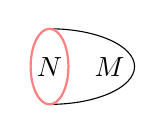
\begin{tikzpicture}[scale=0.6, baseline=(x.base)]    \node (x) at (0,0) {\vphantom{x}};
        \def\bdyradius{0.8cm}
        
        \draw (0,-\bdyradius) arc[start angle=-90,end angle=90,x radius=1.8cm,y radius=\bdyradius] node[left=0.1,pos=0.5] {$M$};
        \draw[thick, red!50] (0,0) node[black] {$N$} circle[x radius=0.4cm,y radius=\bdyradius];
        
    \end{tikzpicture}
  \right)
  \in  \mathcal{H}_{N}.
\end{equation}
\end{itemize}
This expresses the path integral quantization on $M$ with boundary.
Recall that if one has a spacetime manifold with boundary, one needs
to impose a boundary condition on fields on the boundary, and it leads
to the state vector associated to the boundary condition by path integral
expression, namely let $\varphi$ be a fixed field configuration on
$N$, 
\begin{equation}
  Z\left(M;\varphi\right)  =  \int_{X\mid_{N}=\varphi}\mathcal{D}X \, e^{-S\left(X\right)} \,  \in  \mathcal{H}_{N}.
\end{equation}
 In other words, the quantum state at a generic time $t$ is given
by the path integral of the Boltzmann weight over all the classical
fields with time $<t$. 


%FIGURE
\begin{figure}
\centering
  \subfloat[\label{fig:one_bdy}]{
    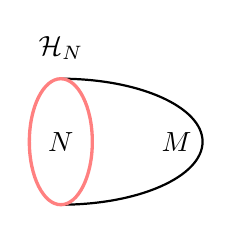
\begin{tikzpicture}[scale=1] %, baseline=(x.base)]    \node (x) at (0,0) {\vphanton{x}};
        \def\bdyradius{0.8cm}
        
        \draw[thick] (0,-\bdyradius) arc[start angle=-90,end angle=90,x radius=1.8cm,y radius=\bdyradius] node[left=0.3,pos=0.5] {$M$};
        \draw[very thick, red!50] (0,0) node[black] {$N$} circle[x radius=0.4cm,y radius=\bdyradius] node[above=\bdyradius+0.1cm, black] {\normalsize$\mathcal{H}_N$};
        
    \end{tikzpicture}
  }
\qquad\qquad
  \subfloat[\label{fig:two_bdy}]{
    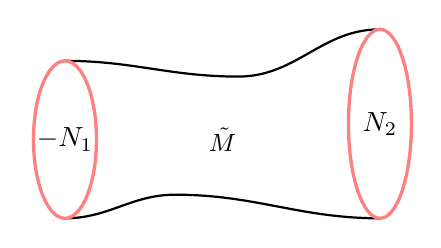
\begin{tikzpicture}[scale=1] %, baseline=(x.base)]    \node (x) at (0,0) {\vphanton{x}};
        \def\bdyradius{1cm}
        
        \draw[thick] (0,-\bdyradius) to[out=0,in=180] (1.4cm,0.3cm-\bdyradius) to[out=0,in=180] (4cm,0.2cm-\bdyradius*1.2);
        \draw[thick] (0,\bdyradius) to[out=0,in=180] (2.2cm,-0.2cm+\bdyradius) to[out=0,in=180] (4cm,0.2cm+\bdyradius*1.2);
        
        \draw[very thick, red!50] (0,0) node[black] {$-N_1$} circle[x radius=0.4cm,y radius=\bdyradius];
        \draw[very thick, red!50] (4,0.2) node[black] {$N_2$} circle[x radius=0.4cm,y radius=\bdyradius*1.2];
        
        \node at (2,0) {\small$\tilde M$};
        
    \end{tikzpicture}
  }
  \caption{one-boundary and two-boundary cases.}
  \label{fig:mfd_w_bdys}
\end{figure}


These data are subject to the following assignments: 
\begin{enumerate}
  \item (involutory) Let $-N$ denote a manifold $N$ with the opposite orientation,
then 
\begin{equation}
  \mathcal{H}_{-N}  =  \mathcal{H}_{N}^{*},
\end{equation}
 where $\mathcal{H}_{N}^{*}$ is the dual to $\mathcal{H}_{N}$. 
  \item (multiplicative) If $N$ is a disjoint union of two $d$-dimensional
closed manifolds $N_{1}$ and $N_{2}$, then the vector space associated
on it is factorized to a tensor product: 
\begin{equation}
  \mathcal{H}_{N_{1}\sqcup N_{2}}  =  \mathcal{H}_{N_{1}}  \otimes  \mathcal{H}_{N_{2}}.
\end{equation}
 This is really natural in the physical point of view. This condition
means that if we have two physical systems defined on spatially disjoint
union $N_{1}\sqcup N_{2}$, then the space of states is represented
as the tensor product of each state space. Also, from the conditions
so far one finds that if ($d+1$)-dimensional manifold $M'$ has two
boundaries such that 
\begin{equation}
  \partial M'  =  -N_{1}\sqcup N_{2},
\end{equation}
then $Z$ defines a linear map
\begin{equation}
  Z\left(M'\right)
  =
  Z\left(
    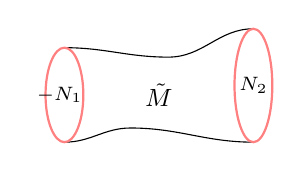
\begin{tikzpicture}[scale=0.6, baseline=(x.base)]    \node (x) at (0,0) {\vphantom{x}};
        \def\bdyradius{1cm}
        
        \draw (0,-\bdyradius) to[out=0,in=180] (1.4cm,0.3cm-\bdyradius) to[out=0,in=180] (4cm,0.2cm-\bdyradius*1.2);
        \draw (0,\bdyradius) to[out=0,in=180] (2.2cm,-0.2cm+\bdyradius) to[out=0,in=180] (4cm,0.2cm+\bdyradius*1.2);
        
        \draw[thick, red!50] (0,0) circle[x radius=0.4cm,y radius=\bdyradius];\node[black] at (-0.1,0) {\scriptsize $-N_1$};
        \draw[thick, red!50] (4,0.2) node[black] {\scriptsize $N_2$} circle[x radius=0.4cm,y radius=\bdyradius*1.2];
        
        \node at (2,0) {\small$\tilde M$};
        
    \end{tikzpicture}
  \right)
  \in  \mathrm{Hom}_{\mathbb{C}}\left(\mathcal{H}_{N_{1}},\mathcal{H}_{N_{2}}\right),
\end{equation}
 namely, for a cobordism between $N_{1}$ and $N_{2}$, we have a
linear map between $\mathcal{H}_{N_{1}}$ and $\mathcal{H}_{N_{2}}$.
This defines a time evolution, or transition amplitude, between the
states in $\mathcal{H}_{N_{1}}$ and $\mathcal{H}_{N_{2}}$. When
the field theory has a Hamiltonian, $Z\left(M'\right)$ may correspond
to the time evolution operator 
\begin{equation}
  Z\left(M'\right):=e^{-tH}:\mathcal{H}_{N_{1}}\longrightarrow\mathcal{H}_{N_{2}}.
\end{equation}
Since canonical quantization is a procedure to make an assignment
of Hilbert spaces and the time evolution on them, as we saw in QM,
this association of linear maps gives the other half of canonical
quantization. %
%\begin{comment}
%Perhaps no need this part
%\end{comment}
One can also explicitly express $Z\left(M'\right)$ in the path integral
expression by the Feynman kernel (also as known as propagator or Green's
function). Suppose we have an initial state $\Psi_{0}\in\mathcal{H}_{N_{1}}$,
then the state $\Psi_{t}\in\mathcal{H}_{N_{2}}$ at time $t$ is expressed
by
\begin{align}
  \Psi_{t}\left(\varphi_{t}\right) 
  & =\left(e^{-tH}\Psi_{0}\right)  \left(\varphi_{t}\right)  \nonumber \\
  & =\int K\left(\varphi_{t},\varphi_{0}\right)\Psi_{0}\left(\varphi_{0}\right)\mathcal{D}\varphi_{0},
\end{align}
 where 
\begin{equation}
  K\left(\varphi_{t},\varphi_{0}\right)  
  =\int_{X\mid_{N_{1}}=\varphi_{0}}^{X\mid_{N_{2}}  
  =\varphi_{t}}\mathcal{D}X\,e^{-S\left(X\right)}.
\end{equation}
  \item For two cobordisms such that 
\begin{equation}
  \partial M_1 =  -N_{1}\sqcup N_{2},  \quad  \partial M_2  =  -N_{2}\sqcup N_{3},
\end{equation}
 it follows that 
\begin{equation}
  Z\left(M_1  \cup_{N_{2}} M_2  \right)  =  Z\left(M_2\right)Z\left(M_1\right),
\end{equation}
where the cobordisms $M_1$ and $M_2$ are glued along $N_{2}$ by a
certain diffeomorphism on $N_{2}$. This asserts that the linear maps
are transitive when we compose cobordisms. This is nothing but the
physical requirement that the time evolution is compatible with the
cutting and gluing the manifolds. 
  \item Given $N=\emptyset$ as an empty $d$-dimensional manifold, then the
associated vector space is one-dimensional:
\begin{equation}
  Z\left(\emptyset\right)  =  \mathbb{C}.
\end{equation}
This is a non-triviality condition. Therefore, for each ($d+1$)-dimensional
manifold $M$ without boundary, $\partial M=\emptyset$, $Z$ assigns
a number: 
\begin{equation}
  Z\left(M\right)  \in  \mathbb{C}.
\end{equation}
 This number associated to a closed ($d+1$)-dimensional manifold
is called the partition function. Not only is it an important quantity
physically, but it also has mathematical applications, such as giving
a topological invariant of the closed manifold $M$. 
\item Let $I$ be an interval, then for each cylinder $M=N\times I$, the
linear map on $\mathcal{H}_{N}$ is trivial: 
\begin{equation}
  Z\left(N\times I\right)  =  \mathrm{id}_{\mathcal{H}_{N}}.
\end{equation}
 Since in a topological theory manifolds diffeomorphic to each other
should be considered as the identical, each cobordism class defines
a linear map. This means that the addition of a cylinder is a trivial
operation, the associated linear map is the identity. This condition
is another major difference from ordinary QFTs. For example, for ($2+1$)-dimensional
Chern-Simons theory one can explicitly see its Hamiltonian is identically
$0$ and hence the time evolution of Chern-Simons theory is trivial. 
\end{enumerate}
%
This is all the assignments for Atiyah's TQFT. Although we gave the
path integral expressions at the explanation of the physical meanings
for some conditions, the axioms themselves are really the basis for
the rigorous mathematical definition of $Z$. One can actually take
an equivalent definition of TQFT in slightly different axioms. For
more details, see the original paper by Atiyah. 

At first sight, this might look a little bit complicated and too abstract.
This definition, however, is really natural and works quite well in
a sense that it gives a kind of ``homomorphism'' between geometry
and algebra: 
\[
Z:\text{`geometry'}\longrightarrow\text{`algebra'}.
\]
 In fact, all in all the axioms of Atiyah's TQFT define a functor
from the category of ($d+1$)-dimensional cobordisms to the category
of finite-dimensional $\mathbb{C}$-vector spaces:%
%
\footnote{What is more, the category of cobordisms and the category of vector
spaces are endowed with the product structures, that is, taking disjoint
union and taking tensor product, which are really symmetric operations.
As such, the functor between them is keeping such structures and then
called symmetric monoidal functor. }
% 
\begin{equation}
  Z:\mathrm{Bord}_{d+1}  \longrightarrow  \mathrm{Vect}_{\mathbb{C}}.
\end{equation}
 TQFT luckily has a mathematical precise definition. For a general
QFT, i.e.~not TQFT, in many cases there is no precise definition as
we saw the examples of the construction of $Z$. However, a QFT is
generically expected to be characterized by some functor from the
geometric structure of spacetime manifolds to the algebraic description
of physical states and observables. 





\subsection{Lattice model as discrete QFT}

Now let us move on to the discussion on lattice model. First of all,
let us begin with the question of ``what is lattice model?'' Probably
there is no unique definition of lattice model. We here would like
to characterize lattice model by a discrete version of QFT. What we
have learnt in the previous subsection is that a ($d+1$)-dimensional
QFT may be defined by an appropriate functor $Z_{\mathrm{Q}}^{d+1}$,
which produces a number for each ($d+1$)-dimensional closed manifold
$M$: 
\begin{equation}
  Z_{\mathrm{Q}}^{d+1}\left(M\right)  \in  \mathbb{C},
\end{equation}
 which is called the partition function of the model, and $Z_{\mathrm{Q}}^{d+1}$
satisfies additional some reasonable conditions for each QFT of interest. 

We introduce lattice model in the same way. For a ($d+1$)-dimensional
closed lattice $L$, a ($d+1$)-dimensional lattice model is defined
by $Z_{\mathrm{L}}^{d+1}$, which produces a number 
\begin{equation}
  Z_{\mathrm{L}}^{d+1}\left(L\right)  \in  \mathbb{C},
\end{equation}
which is again called the partition function, and $Z_{\mathrm{L}}^{d+1}$
satisfies additional some reasonable conditions. The most typical
example of lattice model in particle physics is lattice gauge theory
or lattice QCD.%
%
\footnote{For sure, for any field theories when one computes a physical quantity
on a computer, one needs to discretize the theory and put it on a
lattice. In this sense, numerical analysis of field theory is always
regarded as a lattice model. }
%
 For such theories, it is really clear that the model is defined by
a discrete version of QFTs; One compactifies the spacetime manifold
$\mathbb{R}^{4}$ to four-torus $T^{4}$, and then discretize the
theory and put it on a lattice on the torus. 

Throughout the paper, we will consider only $d=0$ or $1$ case of
lattice model, and we call each case as 1d or 2d lattice model. To
prepare for the discussion of integrability, we take the prominent
example of statistical lattice model called the Ising model. We first
briefly review the generality of the Ising model and compare with
field theory, and then introduce the transfer matrix which is essentially
a time evolution operator in a discrete quantum system. 





\subsubsection{Prominent example -- the Ising model}

The Ising model is a very good introduction to integrable lattice
model. The 1d and 2d Ising model is known to be exactly solvable,
whose meaning we will clarify in a moment, and it is called integrable.
To see the generality of the Ising model, we first define 2d lattice
and spin configurations on it. 

Define a 2d periodic lattice on two-torus $T^{2}$ by 
\begin{align}
L 
  & :=  \mathbb{Z}_{M}\times\mathbb{Z}_{N}  \nonumber \\
  & =   \left\{ 1,\ldots,M\right\} \times\left\{ 1,\ldots,N\right\} .
\end{align}
 A spin configuration on the lattice $L$ is defined by a map
\begin{equation}
  \mathbf{s}  :  L  \longrightarrow  \left\{ +1,-1\right\} ,
\end{equation}
where usually $+1$ is called up spin and $-1$ down spin. The
map defines up or down spin at each site of the lattice $L$. So it
can also be thought of as an assignment of $+1$ or $-1$ on all the
sites of the lattice $L$. We often denote the spin at each site by
its image $s_{I} := \mathbf{s}\left(I\right),\,I\in L$. Let $S\left(L\right)$
be the set of all the spin configurations. Since spin configurations
are defined on the $M\times N$ periodic lattice, the number of elements
in $S\left(L\right)$ is $2^{MN}$. In other words, the number of
all the allowed configurations of spins on the lattice $L$ is $2^{MN}$.

For each spin configuration $\mathbf{s}\in S\left(L\right)$, define
the energy functional of the Ising model by
\begin{align}
  E_{\mathrm{Ising}}\left(\mathbf{s}\right) 
  & =   -J  \sum_{\left\langle I,I'\right\rangle } s_{I}s_{I'}  \nonumber \\
  & :=  -J  \left( \sum_{i,j=1}^{M,N}s_{ij}s_{i,j+1}+\sum_{i,j}s_{ij}s_{i+1,j} \right),
\end{align}
 where the $s_{ij}=s_{i+M,j}=s_{i,j+N}$, and $J\in\mathbb{R}_{>0}$
is a constant parameter. This is one of the simplest spin systems,
in which only the nearest neighbor spins have interactions. From this
energy functional, the partition function of the Ising model is defined
by 
\begin{equation}
  Z\left(L,E_{\mathrm{Ising}};\beta\right)  :=  \sum_{\mathbf{s}\in S\left(L\right)}  e^{-\beta E_{\mathrm{Ising}}\left(\mathbf{s}\right)},
\end{equation}
 where $\beta\in\mathbb{R}_{\geq0}$ is an inverse temperature. The
summand is generically called the Boltzmann weight as well as in field
theory. In this expression, one recognizes that the right-hand side
is a discrete version of path integral expression in field theory.
The energy functional is corresponding to the action functional of
a field theory, $\beta^{-1}$ is the Planck's constant, and the sum
over all the spin configurations is the path integral over all the
field configurations. Given a periodic lattice $L$, the partition
function returns a number, which is a discrete version of the partition
function of QFT which returns a number as well if a closed manifold
$M$ is given. For later use, define another quantity called the free
energy, 
\begin{equation}
  f\left(\beta\right)  :=  -\frac{1}{\beta}\frac{1}{MN}\log Z\left(\beta\right),
\end{equation}
 where $Z\left(\beta\right)$ is the partition function defined above. 

%\begin{comment}
%Perhaps no need this part
%\end{comment}
According to the general theory of statistical mechanics, the probability
that a configuration $\mathbf{s}$ with energy $E\left(\mathbf{s}\right)$
will be realized is given by the canonical ensemble%
%
\footnote{To the end of this subsection, we argue for a general energy functional,
but the reader may assume the Ising model. }
%
\begin{equation}
p\left(\mathbf{s}\right)  =  \frac{1}{Z}e^{-\beta E\left(\mathbf{s}\right)},
\end{equation}
 where $Z$ is the partition function introduced above. In lattice
model, a physical observable is in general given by a functional on
the space of spin configurations: 
\begin{equation}
  \mathcal{O}  :  S\left(L\right)  \longrightarrow  \mathbb{R},
\end{equation}
and its expectation value is given by the canonical ensemble as 
\begin{equation}
\left\langle \mathcal{O}\right\rangle _{p}  
  :=\sum_{\mathbf{s}\in S\left(L\right)}\mathcal{O}\left(\mathbf{s}\right)p\left(\mathbf{s}\right)  
    =\frac{1}{Z}\sum_{\mathbf{s}\in S\left(L\right)}\mathcal{O}\left(\mathbf{s}\right)e^{-\beta E\left(\mathbf{s}\right)}.
\end{equation}
 In particular, an energy functional is an example of physical observable,
\begin{equation}
\frac{1}{MN}\left\langle E\right\rangle _{p}
  =\frac{1}{MN}\frac{1}{Z}\sum_{\mathbf{s}\in S\left(L\right)}E\left(\mathbf{s}\right)e^{-\beta E\left(\mathbf{s}\right)},
\end{equation}
 which is obtained from the derivative of the free energy, 
\begin{equation}
\frac{1}{MN}\left\langle E\right\rangle _{p}=\frac{\partial}{\partial\beta}\left(\beta f\left(\beta\right)\right).
\end{equation}

Generally speaking, the free energy provides us all the information
of the system. For example, the state most likely to happen is given
by the critical point of the free energy, and we can in principle
compute physical quantities such as expectation value of energy, fluctuation,
specific heat, and so on. To make a lattice model as a physically
meaningful system, however, one needs to take the thermodynamic limit;
$M,N\rightarrow\infty$. Therefore, in this sense, integrability of
lattice model is characterized by the calculability of an exact free
energy at the thermodynamic limit. This may be rephrased by the calculability
of the partition function as well. Based on these argument, we shall
see the integrability of the Ising model in the next subsection. 





\subsubsection{Transfer matrix and integrability}

It is well known that 1d and 2d Ising model is exactly solvable in
the sense that one can exactly compute its free energy in the thermodynamic
limit. Both 1d and 2d cases are solved by so-called the method of
transfer matrix. To see this, for simplicity in this section we consider
1d Ising model. 

The setup is almost the same as in the 2d case. A 1d lattice on torus
and a spin configuration is defined by
\begin{equation}
L_{1d}  =  \mathbb{Z}_{N}  =  \left\{ 1,\ldots,N\right\} ,
\end{equation}
%
\begin{equation}
\mathbf{s}  :  L_{1d}  \longrightarrow  \left\{ \pm1\right\} .
\end{equation}
Define the energy functional of 1d Ising model by 
\begin{equation}
  E_{1d\,\mathrm{Ising}}\left(\mathbf{s}\right)  =  -J\sum_{i=1}^{N}s_{i}s_{i+1},\quad\,s_{N+1}=s_{1}.
\end{equation}
 Then the partition function of 1d Ising model is given as 
\begin{align}
  Z\left(L_{1d},E_{\mathrm{1d}};\beta\right) 
  & :=  \sum_{\mathbf{s}}  e^{-\beta E_{1d}\left(\mathbf{s}\right)}\nonumber \\
  & =   \sum_{s_{1},\ldots,s_{N}=\pm1}  e^{Ks_{1}s_{N}}  \cdots  e^{Ks_{3}s_{2}}e^{Ks_{2}s_{1}},
\end{align}
 where $K:=\beta J$. 
 
 
%FIGURE
\begin{figure}
\centering
  \subfloat[\label{fig:Ising_c}]{
      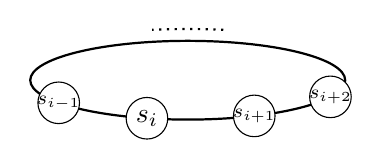
\begin{tikzpicture}[yscale=0.25, spins/.style={draw, fill=white, shape=circle}] %, baseline=(x.base)]    \node (x) at (0,0) {\vphantom{x}};
        
        \draw[thick] (0,0) circle[radius=2cm];
        \draw[thick, dotted] (80:2.6) arc[start angle=80, end angle=100, radius=2.6];
        
        %\draw[fill=white] (215:2) node {$s_{i-1}$} circle[radius=0.3cm];
        %\draw[fill=white] (255:2) node {$s_i$} circle[radius=0.3cm];
        %\draw[fill=white] (295:2) node {$s_{i+1}$} circle[radius=0.3cm];
        %\draw[fill=white] (335:2) node {$s_{i+2}$} circle[radius=0.3cm];
        
        
        \node[spins] at (215:2) {\vphantom{X}};\node at (215:2) {\scriptsize $s_{i-1}$};
        \node[spins] at (255:2) {\vphantom{X}};\node at (255:2) {$s_i$};
        \node[spins] at (295:2) {\vphantom{X}};\node at (295:2) {\scriptsize $s_{i+1}$};
        \node[spins] at (335:2) {\vphantom{X}};\node at (335:2) {\scriptsize $s_{i+2}$};
        
    \end{tikzpicture}
  }
  \qquad\qquad
  \subfloat[\label{fig:Ising_q}]{
      \begin{tikzpicture}[yscale=0.25, spins/.style={draw, fill=white, shape=circle}] %, baseline=(x.base)]    \node (x) at (0,0) {\vphantom{x}};
        
        \draw[thick] (0,0) circle[radius=2cm];
        \draw[thick, dotted] (80:2.6) arc[start angle=80, end angle=100, radius=2.6];
        
        \node (si-1) at (215:2) {\large$\bullet$};\node (i-1) at ($(si-1)+(0.1,1.4)$) {$\mathbb{C}^2$};
        \node (si) at (255:2) {\large$\bullet$};\node (i) at ($(si)+(0.1,1.5)$) {$\mathbb{C}^2$};
        \node (si+1) at (295:2) {\large$\bullet$};\node (i+1) at ($(si+1)+(0,1.5)$) {$\mathbb{C}^2$};
        \node (si+2) at (335:2) {\large$\bullet$};\node (i+2) at ($(si+2)+(-0.2,1.2)$) {$\mathbb{C}^2$};
        
%        \draw[thick, arrows=-to] (i-1) to node[below left] {$T$} (i);
%        \draw[thick, arrows=-to] (i) to node[below] {$T$} (i+1);
%        \draw[thick, arrows=-to] (i+1) to node[below right] {$T$} (i+2);
        
    \end{tikzpicture}
  }
  \caption{(a) Classical Ising spin chain. (b) Quantum states at each site.}
  \label{fig:1dIsing}
\end{figure}


 Let us now introduce the \emph{transfer matrix},
\begin{equation}
  T  :=  \left(e^{Kss'}\right)_{s,s'=\pm1}  
    =
    \left(\begin{array}{ll}
  e^{K}  &  e^{-K}  \\
  e^{-K}  &  e^{K}
\end{array}\right),
\end{equation}
 where the indices of row and column are specified by $+1$ and $-1$,
respectively. Using this matrix $T$, the partition function is rewritten
as
\begin{equation}
  Z\left(\beta\right)
    =\sum_{s_{1},\ldots,s_{N}=\pm1}  T_{s_{1}s_{N}}  \cdots  T_{s_{3}s_{2}}T_{s_{2}s_{1}}.
\end{equation}
 By definition of matrix multiplication, the partition function is
eventually given by a trace: 
\begin{align}
  Z\left(\beta\right)  
  & =  \sum_{s_{1}=\pm1}\left(T^{N}\right)_{s_{1}s_{1}}  \nonumber \\
  & =  \mathrm{Tr}_{\mathbb{C}^{2}}\left(T^{N}\right).
\end{align}
 This expression tells us that we have the quantum Hilbert space $\mathbb{C}^{2}$
at the boundary of each 1d segment, and the transfer matrix $T$ sends
a state to the adjacent site, which is the discrete ``time evolution''
of this system; $\log T\propto$ Hamiltonian as we saw in 1d QFT in
section (what is QFT?). This corresponds to the analogue of Hamiltonian
or operator formalism in field theory. In operator formalism, spins
are replaced by the Pauli matrices, and original classical up spin
and down spin are replaced by the eigenvalues and eigenvectors of
the Pauli matrix $\sigma^{z}$. Further, the non-commutativity is
now manifest in a way that the spins and their time evolution is given
by matrices, this is the consequence of quantization. 

In the expression above of the partition function, let us consider
the thermodynamic limit $N\rightarrow\infty$. The eigenvalues of
$T$ are easily obtained and let them be $\lambda_{0}>\lambda_{1}$,
then we have the free energy
\begin{align}
-\beta f\left(\beta\right)  
  & =  \lim_{N\rightarrow\infty}\frac{1}{N}\log Z\left(\beta\right)\nonumber \\
  & =  \lim_{N\rightarrow\infty}\frac{1}{N}\log\lambda_{0}\left(1+\left(\frac{\lambda_{1}}{\lambda_{0}}\right)^{N}\right)\nonumber \\
  & =  \log\lambda_{0}.
\end{align}
 We conclude that the free energy in the thermodynamic limit is just
given by the largest eigenvalue of the transfer matrix. Again, integrability
of lattice model is rephrased as 
\begin{align*}
 &  \textrm{One can exatly find the eigenvalues of transfer matrix}\\
 &  \Rightarrow  \,  \textrm{Can exactly compute the free enrgy}\\
 &  \Rightarrow  \,  \textrm{The system is integrable. }
\end{align*}

The transfer matrices of 1d and 2d Ising model are diagonalizable
and one can exactly find their eigenvectors and eigenvalues using,
for example, algebraic Bethe ansatz. In this sense, 1d and 2d Ising
model are said to be integrable, or exactly solvable. Then, a natural
question arises; when can we diagonalize the transfer matrix of a
lattice model? This actually leads to the most fundamental answer
to the question of ``what is integrable model.'' A canonical answer
is \emph{Yang-Baxter equation}. When the Boltzmann weight with spectral
parameters, which take values in a Riemann surface, satisfies the
Yang-Baxter equation, the lattice model is integrable. We will give
an explanation of this definition of integrability in next subsection
in some detail, with its origin from TQFT with extra dimensions. 


%FIGURE
%\begin{figure}[tbp]
%\centering
%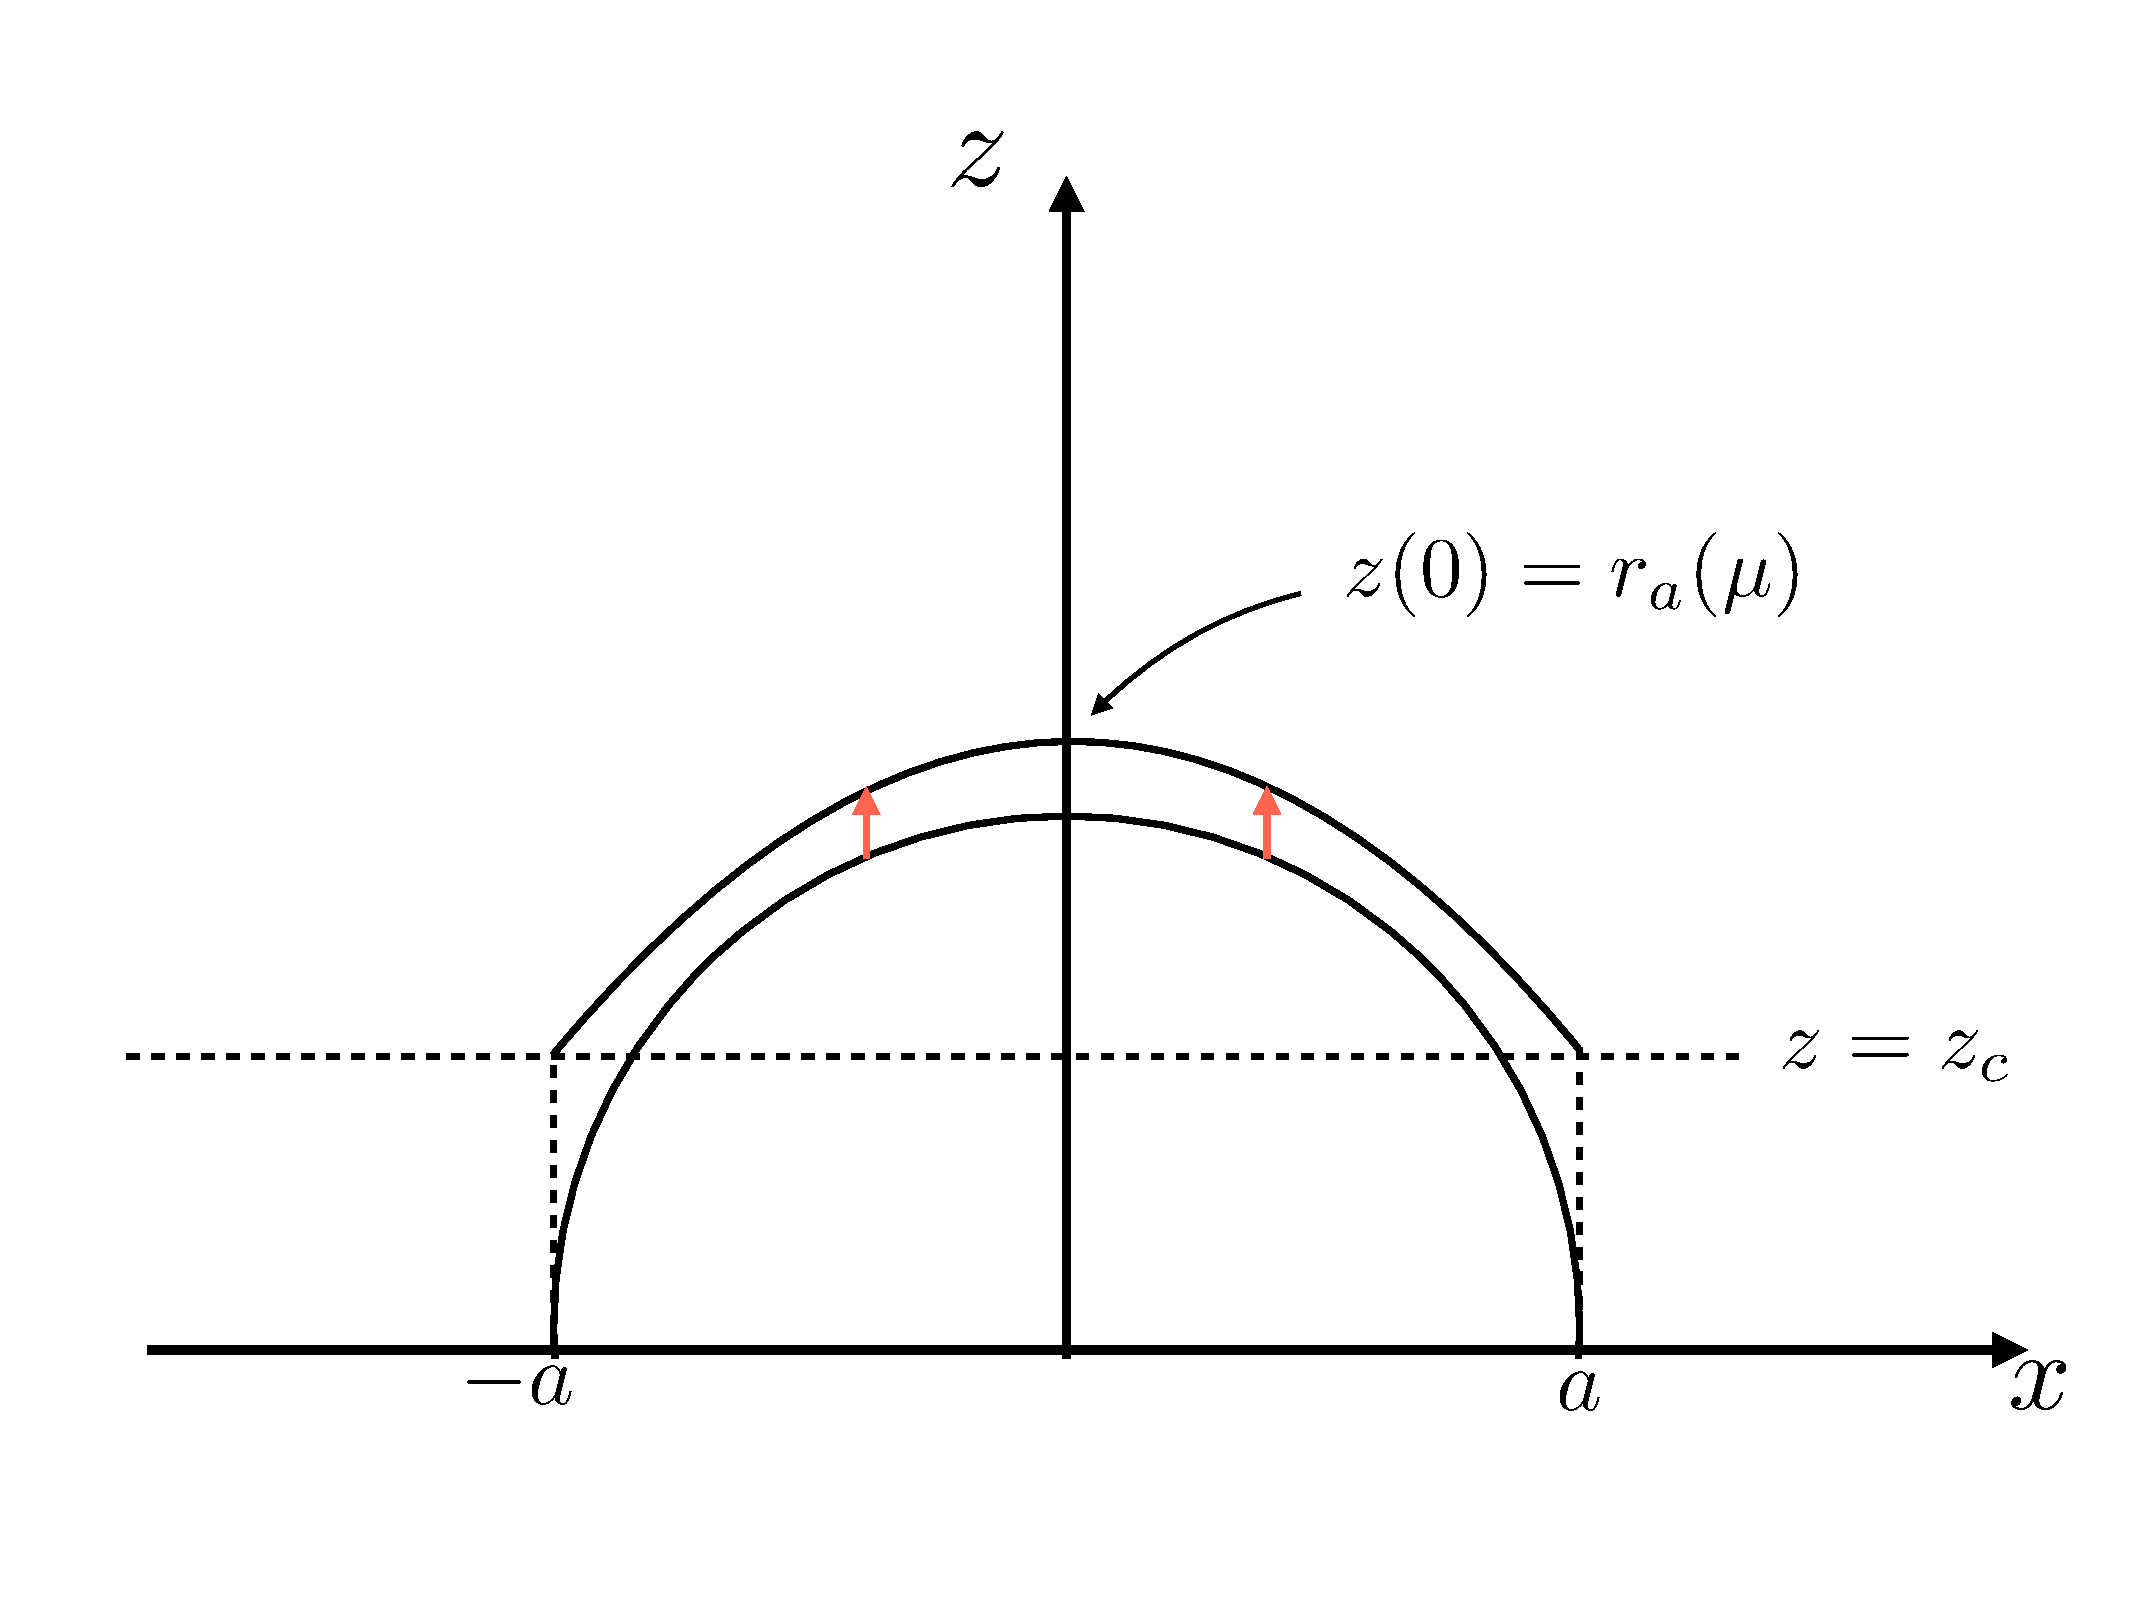
\includegraphics[width=6cm, trim=5cm 4cm 5cm 2cm]{fig/EE1.pdf}
%\caption{A deformed geodesic in the $T\bar{T}$ deformed geometry. }
%\label{fig:deformed}
%\end{figure}




\subsection{Integrability from TQFT in extra dimensions}

In this section we provide a general discussion to relate four-dimensional
supersymmetric gauge theories and integrable lattice models. We clarify
that such a correspondence between gauge theories and lattice models
emerges from a TQFT in extra dimensions. We first give a step-by-step
explanation from two-dimensional TQFT to integrable lattice model,
and then put the argument in the setup of brane tilings. Branes in
string theory are powerful enough to yield the systematic method to
relate a class of supersymmetric gauge theories with integrable lattice
models, as we will see. To begin with, we present a general prescription
of brane constructions at a formal level. Concrete setups and more
details will be given in later sections. 
The discussion in this subsection is mainly based on \cite{Yagi:2016oum}. 

\subsubsection{Lattice models from TQFTs with line operators}

Suppose that we have a two-dimensional TQFT $\mathsf{T}$ on a two-torus
$T^{2}$ equipped with line operators $\mathcal{L}_{i}$, $i=1,\ldots,l$.
Wrap them around one-cycles $C_{i}$ on the torus in such a way that
they form an $m\times n$ lattice. We wish to consider the correlation
function of this configuration of line operators. To compute it, our
strategy is to break up the torus into pieces and perform in turn
the path integral piecewise. Then the original correlation function
is reconstructed by combining these pieces.%
%
\footnote{In the following, we will compute the correlation function by embedding
the closed TQFT with line operators into an open/closed TQFT with
line operators, or defect TQFT; see e.g.~\cite{Moore:2006dw,Carqueville:2016nqk}. }
%

Let us consider the following piece of surface which contains an intersection
of two line operators $\mathcal{L}_{i}$ and $\mathcal{L}_{j}$: 
\begin{equation}
  \label{eq:piece_of_lines}
    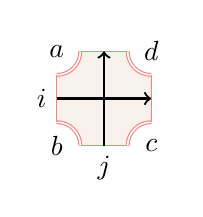
\begin{tikzpicture}[scale=0.6, baseline=(x.base)]
        \node (x) at (0,0) {\vphantom{x}};
        
        \draw[color=red!50, fill=brown!10] (-1,-1) rectangle (1,1);
        
        \fill[color=white] (-1,1) circle (0.5);  \node (a) at (-1,1) {$a$};
        \draw[draw=red!50, double]  (-1,0.5) arc (-90:0:0.5);
        \fill[color=white] (-1,-1) circle (0.5);  \node (b) at (-1,-1) {$b$};
        \draw[draw=red!50, double]  (-1,-0.5) arc (90:0:0.5);
        \fill[color=white] (1,-1) circle (0.5);  \node (c) at (1,-1) {$c$};
        \draw[draw=red!50, double]  (1,-0.5) arc (90:180:0.5);
        \fill[color=white] (1,1) circle (0.5);  \node (d) at (1,1) {$d$};
        \draw[draw=red!50, double]  (1,0.5) arc (-90:-180:0.5);
        
        \draw[thick, ->] (-1,0) node[left] {$i$} -- (1,0);
        \draw[thick, ->] (0,-1) node[below] {$j$} -- (0,1);
        
    \end{tikzpicture}
  \quad .
\end{equation}
 If one thinks of the above picture as the world-sheet of two scattering
open strings, one can regard the above picture as follows: The endpoints
of the open strings sweep out the double-lined arcs, on which D-branes
are there and the boundary conditions (Chan-Paton factors) are specified
by labels $a,\,b,\,c,\,d$. The line operators are the world-lines
of particles associated with the open strings. 


%FIGURE
\begin{figure}
  \centering
  \subfloat[\label{fig:line_on_torus}]{
    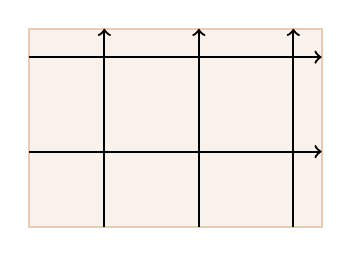
\begin{tikzpicture}[scale=1.2, bdy/.style={draw, color=red, double, fill=white, shape=circle}] %, baseline=(x.base)]
%        \node (x) at (0,0) {\vphantom{x}};
        \def\width{3.1cm}
        \def\height{2.1cm}
        
        \filldraw[color=brown!40, semithick, fill=brown!10] (0,0) rectangle (\width,\height);
        \draw[thick, ->, black] (0.8,0) -- ++(0,\height);\draw[thick, ->, black] (1.8,0) -- ++(0,\height);\draw[thick, ->, black] (2.8,0) -- ++(0,\height);
        \draw[thick, ->, black] (0,0.8) -- ++(\width,0);\draw[thick, ->, black] (0,1.8) -- ++(\width,0);
        
%        \node[bdy] (b1) at (0.3,0.3) {};
%        \node[bdy] (b2) at (1.3,0.3) {};
%        \node[bdy] (b3) at (2.3,0.3) {};
%        \begin{scope}[yshift=1cm]
%        \node[bdy] at (0.3,0.3) {};
%        \node[bdy] at (1.3,0.3) {};
%        \node[bdy] at (2.3,0.3) {};
%        \end{scope}
        
    \end{tikzpicture}
  }
  \qquad
  \subfloat[\label{fig:line_boundary}]{
    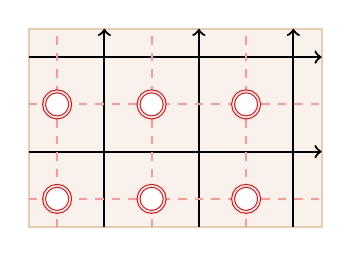
\begin{tikzpicture}[scale=1.2, bdy/.style={draw, color=red, double, fill=white, shape=circle}] %, baseline=(x.base)]
%        \node (x) at (0,0) {\vphantom{x}};
        \def\width{3.1cm}
        \def\height{2.1cm}
        
        \filldraw[color=brown!40, semithick, fill=brown!10] (0,0) rectangle (\width,\height);
        \draw[thick, ->, black] (0.8,0) -- ++(0,\height);\draw[thick, ->, black] (1.8,0) -- ++(0,\height);\draw[thick, ->, black] (2.8,0) -- ++(0,\height);
        \draw[thick, ->, black] (0,0.8) -- ++(\width,0);\draw[thick, ->, black] (0,1.8) -- ++(\width,0);
        
        \draw[thick, color=red!40, dashed] (0.3,0) -- ++(0,\height);\draw[thick, color=red!40, dashed] (1.3,0) -- ++(0,\height);\draw[thick, color=red!40, dashed] (2.3,0) -- ++(0,\height);
        \draw[thick, color=red!40, dashed] (0,0.3) -- ++(\width,0);\draw[thick, color=red!40, dashed] (0,1.3) -- ++(\width,0);
        
        \node[bdy] (b1) at (0.3,0.3) {};
        \node[bdy] (b2) at (1.3,0.3) {};
        \node[bdy] (b3) at (2.3,0.3) {};
        \begin{scope}[yshift=1cm]
        \node[bdy] at (0.3,0.3) {};
        \node[bdy] at (1.3,0.3) {};
        \node[bdy] at (2.3,0.3) {};
        \end{scope}
        
    \end{tikzpicture}
  }
  \qquad
  \subfloat[\label{fig:spin_boundary}]{
    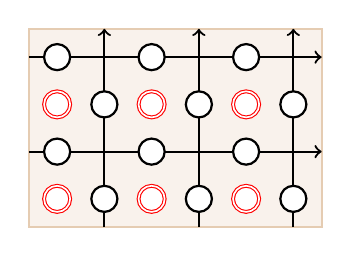
\begin{tikzpicture}[scale=1.2, bdy/.style={draw, color=red, double, fill=white, shape=circle},spin/.style={draw, thick, fill=white, shape=circle}] %, baseline=(x.base)]
%        \node (x) at (0,0) {\vphantom{x}};
        \def\width{3.1cm}
        \def\height{2.1cm}
        
        \filldraw[color=brown!40, semithick, fill=brown!10] (0,0) rectangle (\width,\height);
        \draw[thick, ->, black] (0.8,0) -- ++(0,\height);\draw[thick, ->, black] (1.8,0) -- ++(0,\height);\draw[thick, ->, black] (2.8,0) -- ++(0,\height);
        \draw[thick, ->, black] (0,0.8) -- ++(\width,0);\draw[thick, ->, black] (0,1.8) -- ++(\width,0);
        
        \node[bdy] (b1) at (0.3,0.3) {};\node[bdy] (b2) at (1.3,0.3) {};\node[bdy] (b3) at (2.3,0.3) {};
        \begin{scope}[yshift=1cm]
        \node[bdy] at (0.3,0.3) {};\node[bdy] at (1.3,0.3) {};\node[bdy] at (2.3,0.3) {};
        \end{scope}
        
        \begin{scope}[xshift=0.5cm]
        \node[spin] at (0.3,0.3) {};\node[spin] at (1.3,0.3) {};\node[spin] at (2.3,0.3) {};
        \end{scope}
        \begin{scope}[yshift=0.5cm]
        \node[spin] at (0.3,0.3) {};\node[spin] at (1.3,0.3) {};\node[spin] at (2.3,0.3) {};
        \end{scope}
        \begin{scope}[yshift=1cm]
                \begin{scope}[xshift=0.5cm]
                \node[spin] at (0.3,0.3) {};\node[spin] at (1.3,0.3) {};\node[spin] at (2.3,0.3) {};
                \end{scope}
                \begin{scope}[yshift=0.5cm]
                \node[spin] at (0.3,0.3) {};\node[spin] at (1.3,0.3) {};\node[spin] at (2.3,0.3) {};
                \end{scope}
        \end{scope}
    \end{tikzpicture}
  }
  \caption{Construction of a lattice model from line operators. 
    (a) A lattice of line operators on a torus. 
    (b) The torus with holes obtained by gluing of pieces. 
    (c) The corresponding spin model. }
  \label{fig:TQFTandSpin}
  
\end{figure}


The path integral for the piece \eqref{eq:piece_of_lines} produces a linear map
\begin{equation}
    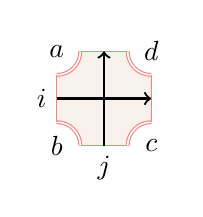
\begin{tikzpicture}[scale=0.6, baseline=(x.base)]
        \node (x) at (0,0) {\vphantom{x}};
        
        \draw[color=red!50, fill=brown!10] (-1,-1) rectangle (1,1);
        
        \fill[color=white] (-1,1) circle (0.5);  \node (a) at (-1,1) {$a$};
        \draw[draw=red!50, double]  (-1,0.5) arc (-90:0:0.5);
        \fill[color=white] (-1,-1) circle (0.5);  \node (b) at (-1,-1) {$b$};
        \draw[draw=red!50, double]  (-1,-0.5) arc (90:0:0.5);
        \fill[color=white] (1,-1) circle (0.5);  \node (c) at (1,-1) {$c$};
        \draw[draw=red!50, double]  (1,-0.5) arc (90:180:0.5);
        \fill[color=white] (1,1) circle (0.5);  \node (d) at (1,1) {$d$};
        \draw[draw=red!50, double]  (1,0.5) arc (-90:-180:0.5);
        
        \draw[thick, ->] (-1,0) node[left] {$i$} -- (1,0);
        \draw[thick, ->] (0,-1) node[below] {$j$} -- (0,1);
        
    \end{tikzpicture}
  \quad \rightsquigarrow \quad
R_{ij}\left(%
  \begin{array}{cc}
        a & d\\
        b & c
  \end{array}%
\right)
  :  V_{ab,i}\otimes V_{bc,j}  \longrightarrow  V_{ad,j}\otimes V_{dc,i} \, ,
\end{equation}
where $V_{ab,i}$ is the space of states of the open string propagating
along $\mathcal{L}_{i}$ with the boundary conditions on the left
and the right ends specified by $a,\,b$, respectively. We call this
map the R-matrix (or R-operator) associated with this decorated surface.
To reconstruct the original configuration of line operators, we glue
pieces together. Gluing them amounts to the composition of R-matrices.
For example, gluing two pieces horizontally gives 
\begin{equation}
    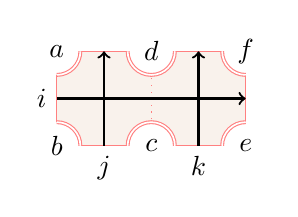
\begin{tikzpicture}[scale=0.6, baseline=(x.base)]
        \node (x) at (0,0) {\vphantom{x}};
        
        \draw[color=red!50, fill=brown!10] (-1,-1) rectangle (3,1);
        \draw[color=red!50, dotted] (1,-1) -- (1,1);
        
        \fill[color=white] (-1,1) circle (0.5);  \node (a) at (-1,1) {$a$};
        \draw[draw=red!50, double]  (-1,0.5) arc (-90:0:0.5);
        \fill[color=white] (-1,-1) circle (0.5);  \node (b) at (-1,-1) {$b$};
        \draw[draw=red!50, double]  (-1,-0.5) arc (90:0:0.5);
        \fill[color=white] (1,-1) circle (0.5);  \node (c) at (1,-1) {$c$};
        \draw[draw=red!50, double]  (1.5,-1) arc (0:180:0.5);
        \fill[color=white] (1,1) circle (0.5);  \node (d) at (1,1) {$d$};
        \draw[draw=red!50, double]  (1.5,1) arc (0:-180:0.5);
        \fill[color=white] (3,-1) circle (0.5);  \node (e) at (3,-1) {$e$};
        \draw[draw=red!50, double]  (3,-0.5) arc (90:180:0.5);
        \fill[color=white] (3,1) circle (0.5);  \node (f) at (3,1) {$f$};
        \draw[draw=red!50, double]  (3,0.5) arc (-90:-180:0.5);
        
        \draw[thick, ->] (-1,0) node[left] {$i$} -- (3,0);
        \draw[thick, ->] (0,-1) node[below] {$j$} -- (0,1);
        \draw[thick, ->] (2,-1) node[below] {$k$} -- (2,1);
        
    \end{tikzpicture}
%  \ =
  \quad \rightsquigarrow \quad
R_{ik}\left(%
  \begin{array}{cc}
        d & e\\
        c & f
  \end{array}%
\right)
  \circ_{V_{dc,i}}
R_{ij}\left(%
  \begin{array}{cc}
        a & d\\
        b & c
  \end{array}%
\right).
\end{equation}

The original configuration is thus obtained by gluing all the pieces.
It, however, still has holes assigned boundary conditions as in figure \ref{fig:line_boundary},
which we must fill by summing over the boundary conditions. To do
this, let us recall that the path integral on a finite-length cylinder
with boundary condition $a$ imposed on one end defines a closed string
state $\left|a\right\rangle $ as known as a boundary state. Similarly,
the path integral on a disk with no insertion of operators defines
a state $\left|1\right\rangle $ on the boundary. 
%, see figures. 
Assume
that we have chosen the set of boundary conditions $B$ to be sufficiently
large so that the state $\left|1\right\rangle $ can be written as
a superposition of boundary states:
\begin{equation}
  \left|1\right\rangle  =  \sum_{a\in B}c_{a}\left|a\right\rangle .
\end{equation}
 Then, the sum over the boundary conditions gives the state $\left|1\right\rangle $
on the boundary of each hole, which is replaced with a disk: 
\begin{equation}
  \sum_{a\in B}  c_a  \left(  ~  a  ~
    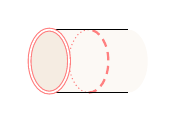
\begin{tikzpicture}[xscale=0.25, yscale=0.4, baseline=(x.base)]
        \node (x) at (0,0) {\vphantom{x}};
        \def\cylinderlength{4cm}
        
        \fill[color=brown!5] (0,-1) arc (-90:90:1) -- ++(\cylinderlength,0) arc (90:-90:1) -- ++(-\cylinderlength,0) -- cycle;
        
        \draw[color=red!50, densely dashed, thick] (\cylinderlength/2,-1) arc (-90:90:1);
        \draw[color=red!50, densely dotted] (\cylinderlength/2,1) arc (90:270:1);
        
        \draw (0,1) -- (\cylinderlength,1);
        \draw (0,-1) -- (\cylinderlength,-1);
        
        \filldraw[color=red!50, double, fill=brown!15] (0,0) circle[radius=1];
        
    \end{tikzpicture}
  \right)  
  =  \sum_{a\in B}  c_a  \left(  ~  \left|a\right\rangle  ~
    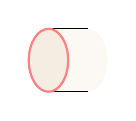
\begin{tikzpicture}[xscale=0.25, yscale=0.4, baseline=(x.base)]
        \node (x) at (0,0) {\vphantom{x}};
        \def\cylinderlength{2cm}
        
        \fill[color=brown!5] (0,-1) arc (-90:90:1) -- ++(\cylinderlength,0) arc (90:-90:1) -- ++(-\cylinderlength,0) -- cycle;
        
        \draw (0,1) -- (\cylinderlength,1);
        \draw (0,-1) -- (\cylinderlength,-1);
        
%        \draw[color=red!50, densely dashed, thick] (\cylinderlength/2,-1) arc (-90:90:1);
%        \draw[color=red!50, densely dotted] (\cylinderlength/2,1) arc (90:270:1);
        
        \filldraw[color=red!50, thick, fill=brown!15] (0,0) circle[radius=1];
        
    \end{tikzpicture}
  \right)  
    =  ~  \left|1\right\rangle  ~
      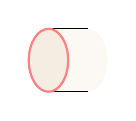
\begin{tikzpicture}[xscale=0.25, yscale=0.4, baseline=(x.base)]
        \node (x) at (0,0) {\vphantom{x}};
        \def\cylinderlength{2cm}
        
        \fill[color=brown!5] (0,-1) arc (-90:90:1) -- ++(\cylinderlength,0) arc (90:-90:1) -- ++(-\cylinderlength,0) -- cycle;
        
        \draw (0,1) -- (\cylinderlength,1);
        \draw (0,-1) -- (\cylinderlength,-1);
        \filldraw[color=red!50, thick, fill=brown!15] (0,0) circle[radius=1];
        
    \end{tikzpicture}
  \ = \ 
    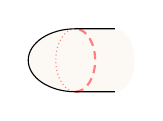
\begin{tikzpicture}[xscale=0.25, yscale=0.4, baseline=(x.base)]
        \node (x) at (0,0) {\vphantom{x}};
        \def\cylinderlength{2cm}
        
        \fill[color=brown!5] (0,-1)  arc[start angle=270,end angle=90,x radius=2.4,y radius=1] -- ++(\cylinderlength,0) arc (90:-90:1) -- ++(-\cylinderlength,0) -- cycle;
        
        \draw[color=red!50, densely dashed, thick] (0,-1) arc (-90:90:1);
        \draw[color=red!50, densely dotted] (0,1) arc (90:270:1);
        
        \draw (\cylinderlength,-1) -- (0,-1) arc[start angle=270,end angle=90,x radius=2.4,y radius=1]   -- (\cylinderlength,1);
        
    \end{tikzpicture}
  \quad  .
\end{equation}
 Thus the holes are filled and the original configuration on the torus
is reconstructed. 

Now that we have understood how to reconstruct the correlation function
of line operators in the field theoretic point of view, let us reinterpret
this procedure as an operation in statistical lattice model. Rephrasing
the procedures so far, it is clear that the above configuration defines
a partition function of a statistical spin model. The model has spins
located at two kinds of sites, \tikz{\draw[thick, fill=white] (0,0) circle[radius=0.15cm]} 
and \tikz{\draw[semithick, double, fill=white] (0,0) circle[radius=0.14cm]}. They
correspond to the open string states and the boundary states. A spin
at \tikz{\draw[thick, fill=white] (0,0) circle[radius=0.15cm]} takes values in the chosen basis for the relevant open
string states $V_{ab,i}$, while that at \tikz{\draw[semithick, double, fill=white] (0,0) circle[radius=0.14cm]} is valued
in $B$. The Boltzmann weights for each spin configuration are given
by the matrix elements of R-matrix and the coefficients of boundary
states $c_{a}$. Thus, we conclude that the correlation function of
line operators $\left\{ \mathcal{L}_{i}\right\} $ on the torus coincides
with the partition function of a statistical spin model defined on
the periodic lattice formed by the line operators:
\begin{equation}
  \left\langle \prod_{i=1}^{l}\mathcal{L}_{i}\left(C_{i}\right)\right\rangle_{\mathsf{T},T^{2}}
    =Z_{\mathsf{L}\left(\mathsf{T}\right),\left\{ \mathcal{L}_{i}\left(C_{i}\right)\right\} }.
\end{equation}
$\mathsf{L}\left(\mathsf{T}\right)$ denotes the lattice model arising
from the TQFT $\mathsf{T}$ with the line operators and $\left\{ \mathcal{L}_{i}\left(C_{i}\right)\right\} $
is the lattice formed by line operators $\mathcal{L}_{i}$ wrapping
around $C_{i}$. By this construction, we can view typical examples
of lattice models. 

\subsubsection*{IRF model}

If $\dim V_{ab,i}=1$ for any $a,\,b,\,i$, in this case we can ignore
the spins at \tikz{\draw[thick, fill=white] (0,0) circle[radius=0.15cm]}. We just sum over the boundary conditions
and such a spin system $\mathsf{L}\left(\mathsf{T}\right)$ is called
\emph{interaction-round-a-face model}, or \emph{IRF model} for short.
The spins are placed on the faces of the lattice, and interaction
takes place among four spins surrounding a vertex. The 2d Ising model
actually can be formulated as an IRF model by taking vertex-face correspondence. 


\subsubsection*{Vertex model}

If $B$ consists of a single boundary condition, say $a$, we can
simply write the open string state space by $V_{i}:=V_{aa,i}$, and
the R-matrix is represented only by a crossing of two lines: 
\begin{equation}
  R_{ij}
  =
    \begin{tikzpicture}[scale=0.6, baseline=(x.base)]
        \node (x) at (0,0) {\vphantom{x}};
        
        \draw[thick, ->] (0,0) node[left] {$i$} -- (2,0);
        \draw[thick, ->] (1,-1) node[below] {$j$} -- (1,1);
        
    \end{tikzpicture}
  \quad ,
\end{equation}
\begin{equation}
  R_{ij}  :  V_{i}\otimes V_{j}  \longrightarrow  V_{j}\otimes V_{i} \, .
\end{equation}
The space of states $V_{i}$ can also be thought of as the Hilbert
space of a particle propagating on the line operator $\mathcal{L}_{i}$.
In this case we can ignore the spins at \tikz{\draw[semithick, double, fill=white] (0,0) circle[radius=0.14cm]} since there
is no summation over boundary conditions. This means that the lattice
model $\mathsf{L}\left(\mathsf{T}\right)$ is called a \emph{vertex
model}: Spins are living on the edges of the lattice and interact
with each other at the vertices. 

We can always recast our lattice model into a vertex model by setting
$V_{i}:=\bigoplus_{a,b\in B}V_{ab,i}$, at least formally, and declaring
that all newly introduced R-matrix elements, which correspond to scattering
processes with inconsistent Chan-Paton factors, vanish. We can also
absorb the coefficients $c_{a}$ into the R-matrix elements by appropriate
rescaling. In what follows we implicitly perform this reformulation,
and restrict ourselves to vertex model.

A remarkable aspect of this construction of lattice models is that
it allows us to understand integrability from a higher-dimensional
point of view. This is crucial observation by Costelllo \cite{Costello:2013sla}.
In our lattice model, consider a horizontal line operator $\mathcal{L}_{i}$
intersecting vertical line operators $\mathcal{L}_{j}$, $j=1,\ldots,n$.
Concatenating the R-matrices in this row, we get the row-to-row transfer
matrix: 
\begin{equation}
  T_{i} 
  =
    \begin{tikzpicture}[scale=0.8, baseline=(x.base)]
        \node (x) at (0,0) {\vphantom{x}};
        
        \draw[thick] (0,0.2) to[out=180, in=180] (0,0);
        \draw[thick, ->-=0.24] (0,0) node[left] {$i\,$} -- (3,0);
        \draw[thick] (3,0) to[out=0, in=0] (3,0.2); 
        
        \draw[preaction={draw=white, ultra thick}, thick, loosely dotted] (1.2,0) -- (2.4,0);
        
        \draw[thick, ->] (0.3,-0.4) node[below] {$1$} -- (0.3, 0.6);
        \draw[thick, ->] (0.9,-0.4) node[below] {$2$} -- (0.9, 0.6);
        \draw[thick, ->] (2.7,-0.4) node[below] {$n$} -- (2.7, 0.6);
    
    \end{tikzpicture}
%    \begin{tikzpicture}[yscale=0.8, baseline=(x.base)]
%    \node (x) at (0,0) {\vphantom{x}};
%    
%    \draw[thick] (0,0.2) to [out=180, in=180] (0,0);
%    \draw[thick, ->-=0.35] (0,0) node[left] {$i\,$} -- (1.2,0)  (2.0,0) -- (2.6,0);
%    \draw[thick, loosely dotted] (1.2,0) -- (2.0,0);
%    \draw[thick] (2.6,0) to [out=0, in=0] (2.6,0.2); 
%    
%    \draw[thick, ->] (0.2,-0.4) node[below] {$1$} -- (0.2, 0.6);
%    \draw[thick, ->] (0.8,-0.4) node[below] {$2$} -- (0.8, 0.6);
%    \draw[thick, ->] (2.4,-0.4) node[below] {$n$} -- (2.4, 0.6);
%    
%    \end{tikzpicture}
  \ =  
  \mathrm{Tr}_{V_{i}}\left(R_{i,n}\circ_{V_{i}}\cdots\circ_{V_{i}}R_{i,1}\right).
\end{equation}
 The hooks on the horizontal line are to remind us that the periodic
boundary condition is imposed. This gives an endomorphism of $\bigotimes_{j=1}^{n}V_{j}$
which maps a state just below $\mathcal{L}_{j}$ to another state
above it, namely the transfer matrix defines the time evolution of
this spin system and $\bigotimes_{j=1}^{n}V_{j}$ is the quantum Hilbert
space. In terms of transfer matrices, the partition function is written
as a trace, 
\begin{equation}
  Z_{\mathsf{L}\left(\mathsf{T}\right),\left\{ \mathcal{L}_{i}\left(C_{i}\right)\right\} }  
  =\mathrm{Tr}_{\mathcal{H}}\left(T_{n+m}\cdots T_{n+1}\right),
\end{equation}
 where the trace is taken over the total Hilbert space $\mathcal{H}:=\bigotimes_{j=1}^{n}V_{j}$.
An important point is that the underlying field theory is a TQFT,
and hence a state evolves trivially on a cylinder unless it hits something,
line operators in the present case. 

Now suppose that each line operator depends on a continuous parameter
which is an element of some smooth manifold $S$. This parameter is
called \emph{spectral parameter} of the lattice model. We denote the
spectral parameter of $\mathcal{L}_{i}$ by $u_{i}$, then the R-matrix
and the transfer matrix are rewritten by
\begin{align}
  R_{ij}    &    \longrightarrow R_{ij}\left(u_{i},u_{j}\right),  \\
  T_{i}     &    \longrightarrow T_{i}\left(u_{i};u_{1},\ldots,u_{n}\right).
\end{align}
 To avoid clutter, we fix $u_{1},\ldots,u_{n}$ and suppress them
below. A vertex model is said to be integrable if the transfer matrices
$T_{i}\left(u_{i}\right)$ are meromorphic functions of $u_{i}$ and
commute with each other:
\begin{equation}
    \begin{tikzpicture}[xscale=0.8, yscale=0.6, baseline=(x.base)]
        \node (x) at (0,0.5) {\vphantom{x}};
        
        \draw[thick, ->] (0.3,-0.4) -- (0.3, 1.6);
        \draw[thick, ->] (0.9,-0.4) -- (0.9, 1.6);
        \draw[thick, ->] (2.7,-0.4) -- (2.7, 1.6);
        %arrows do not work somehow by preaction below
        
        \draw[thick] (0,0.2) to[out=180, in=180] (0,0);
        \draw[thick, ->-=0.24] (0,0) node[left] {$i\,$} -- (3,0);
        \draw[thick] (3,0) to[out=0, in=0] (3,0.2); 
        \draw[preaction={draw=white, ultra thick}, thick, loosely dotted] (1.2,0) -- (2.4,0);
        
        \draw[thick, yshift=1cm] (0,0.2) to[out=180, in=180] (0,0);
        \draw[thick, ->-=0.24, yshift=1cm] (0,0) node[left] {$j\,$} -- (3,0);
        \draw[thick, yshift=1cm] (3,0) to[out=0, in=0] (3,0.2); 
        \draw[preaction={draw=white, ultra thick}, thick, loosely dotted, yshift=1cm] (1.2,0) -- (2.4,0);
        
    \end{tikzpicture}
  \ = 
    \begin{tikzpicture}[xscale=0.8, yscale=0.6, baseline=(x.base)]
        \node (x) at (0,0.5) {\vphantom{x}};
        
        \draw[thick, ->] (0.3,-0.4) -- (0.3, 1.6);
        \draw[thick, ->] (0.9,-0.4) -- (0.9, 1.6);
        \draw[thick, ->] (2.7,-0.4) -- (2.7, 1.6);
        %arrows do not work somehow by preaction below
        
        \draw[thick] (0,0.2) to[out=180, in=180] (0,0);
        \draw[thick, ->-=0.24] (0,0) node[left] {$j\,$} -- (3,0);
        \draw[thick] (3,0) to[out=0, in=0] (3,0.2); 
        \draw[preaction={draw=white, ultra thick}, thick, loosely dotted] (1.2,0) -- (2.4,0);
        
        \draw[thick, yshift=1cm] (0,0.2) to[out=180, in=180] (0,0);
        \draw[thick, ->-=0.24, yshift=1cm] (0,0) node[left] {$i\,$} -- (3,0);
        \draw[thick, yshift=1cm] (3,0) to[out=0, in=0] (3,0.2); 
        \draw[preaction={draw=white, ultra thick}, thick, loosely dotted, yshift=1cm] (1.2,0) -- (2.4,0);
        
    \end{tikzpicture}
%\end{equation}
%\begin{equation}
~ \Longleftrightarrow ~ 
\left[T_{i}\left(u_{i}\right) , T_{j}\left(u_{j}\right)\right]  
  =  0,\quad u_{i}\neq u_{j}.
\end{equation}
 When the transfer matrices with different spectral parameters commute,
we can find a series of mutually commuting operators on the total
Hilbert space $\bigotimes_{j=1}^{n}V_{j}$ by Laurent expansion of
the transfer matrix. In particular, they commute with the transfer
matrix, which means they produce an infinite number of conserved quantities.
In fact, the commutativity of transfer matrix implies that one can
find the exact eigenvalues and eigenvectors of the transfer matrix,
as we saw in the Ising model in the previous section. 

The situation considered here, namely the addition of spectral parameters
and commuting transfer matrix, is naturally realized if the TQFT has
``extra dimensions.'' In this scenario, we really start with a higher-dimensional
theory $\tilde{\mathsf{T}}$ formulated on the product space $S\times T^{2}$,
which is topological on the torus $T^{2}$ but not on $S$. We wrap
line operators $\mathcal{L}_{i}$ around $\left\{ u_{i}\right\} \times C_{i}$,
where $u_{i}$ are points on $S$. If one can see only the torus $T^{2}$
and is unaware of the extra dimensions $S$, the theory seems to be
the previous two-dimensional TQFT $\mathsf{T}\cong\tilde{\mathsf{T}}\left[S\right]$
that has parameters taking values in $S$. One finds that line operators
$\mathcal{L}_{i}\left[u_{i}\right]$ wrapping around $C_{i}$ carry
continuous parameters $u_{i}$ in the seemingly two-dimensional theory,
and the correlation function for this configuration of line operators
is given by the partition function of a lattice model $\mathsf{L}\left(\tilde{\mathsf{T}}\left[S\right]\right)$
defined on the lattice $\left\{ \mathcal{L}_{i}\left[u_{i}\right]\left(C_{i}\right)\right\} $. 

For a generic choice of $\left\{ u_{i}\right\} $, the transfer matrices
of the lattice model $\mathsf{L}\left(\tilde{\mathsf{T}}\left[S\right]\right)$
commute since the two horizontal line operators in the above equation
can move freely and interchange their positions owing to the topological
nature along $T^{2}$; no phase transition occurs when they pass each
other as they do not meet in the full spacetime $S\times T^{2}$.
Thus, integrability follows from the existence of extra dimensions,
whose coordinates provide continuous spectral parameters. 

In fact, we can deduce integrability from another point of view. By
the same logic, we have the unitarity relation 
\begin{equation}
    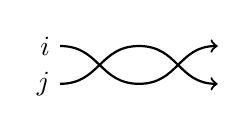
\begin{tikzpicture}[yscale=0.6, baseline=(x.base)]
        \node (x) at (0,0) {\vphantom{x}};
        
        \draw[thick, ->] (0,0.4) node[left] {$i$} to[out=0, in=180] (1,-0.4) to [out=0, in=180] (2,0.4);
        \draw[thick, ->] (0,-0.4) node[left] {$j$} to[out=0, in=180] (1,0.4) to [out=0, in=180] (2,-0.4);
        
    \end{tikzpicture}
  \ =
    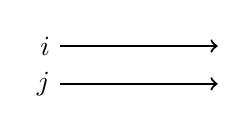
\begin{tikzpicture}[yscale=0.6, baseline=(x.base)]
        \node (x) at (0,0) {\vphantom{x}};
        
        \draw[thick, ->] (0,0.4) node[left] {$i$} -- (2,0.4);
        \draw[thick, ->] (0,-0.4) node[left] {$j$} -- (2,-0.4);
        
    \end{tikzpicture}
\end{equation}
\begin{equation}
   \Longleftrightarrow ~ R_{ji}\left(u_{j},u_{i}\right)R_{ij}\left(u_{i},u_{j}\right)  =  \mathrm{id}_{V_{i}\otimes V_{j}},
\end{equation}
 and the Yang-Baxter equation
\begin{equation}
    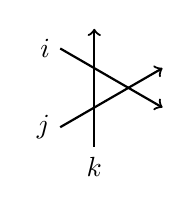
\begin{tikzpicture}[scale=0.5, baseline=(x.base)]
        \node (x) at (30:2) {};
        
        \draw[thick, ->] (0,0) node[left] {$j$} -- ++(30:3);
        \draw[thick, ->] (0,2) node[left] {$i$} -- ++(-30:3);
        \draw[thick, ->] (-30:1) node[below] {$k$} -- ++(0,3);
        
    \end{tikzpicture}
  \ = 
    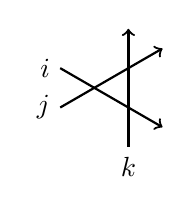
\begin{tikzpicture}[scale=0.5, baseline=(x.base)]
        \node (x) at (30:1) {};
        
        \draw[thick, ->] (0,0) node[left] {$j$} -- ++(30:3);
        \draw[thick, ->] (0,1) node[left] {$i$} -- ++(-30:3);
        \draw[thick, ->] (-30:2) node[below] {$k$} -- ++(0,3);
        
    \end{tikzpicture}
\end{equation}
\begin{equation}
   \Longleftrightarrow ~ R_{ij}\left(u_{i},u_{j}\right)R_{ik}\left(u_{i},u_{k}\right)R_{jk}\left(u_{j},u_{k}\right)  
    =  R_{jk}\left(u_{j},u_{k}\right)R_{ik}\left(u_{i},u_{k}\right)R_{ij}\left(u_{i},u_{j}\right) \, ,
\end{equation}
 where the R-matrix $R_{ij}$ acts on $V_{i}\otimes V_{j}$ as an
intertwiner and trivial on $V_{k}$, etc. From these two relations
we can reproduce the commutativity of the transfer matrix. We should
emphasize that the Yang-Baxter equation is a local condition. When
the Boltzmann weight locally satisfies the Yang-Baxter equation, it
extends to the commutativity of the transfer matrix and hence the
integrability of the model. In this sense, the Yang-Baxter equation
is the fundamental condition of integrability of a lattice model. 


%No need to introduce Sigma?
Before going into the discussion of brane construction, we would like
to generalize the above arguments further higher-dimensional situations.
First of all, replace the two-torus $T^{2}$ with a general two-dimensional
surface $\Sigma$, along which line operators are wrapped. We now
have $S\times\Sigma$, and similarly to the above a lattice model
is defined on $\Sigma$ by line operators with spectral parameters.
Let us consider the case that we really have more extra dimensions
and a higher-dimensional theory is formulated on $S\times M\times\Sigma$
, where $M$ is some smooth manifold. The line operators we had may
descend from extended operators of dimension greater than one. Let
$\mathsf{T}$ again be the new higher-dimensional theory, and suppose
that it is topological on $\Sigma$ and has extended operators $\mathcal{E}_{i}$
whose codimension is greater than $\dim S$. Place $\mathcal{E}_{i}$
on submanifolds of the form $\left\{ u_{i}\right\} \times N_{i}\times C_{i}$.
Since $\mathsf{T}\left[S\times M\right]$ is again regarded as a two-dimensional
TQFT defined on $\Sigma$, the correlation function of the operators
$\mathcal{E}_{i}$ still should coincides with the partition function
of an integrable lattice model $\mathsf{L}\left(\mathsf{T}\left[S\times M\right]\right)$.
The model is defined on the lattice formed by the line operators $\mathcal{E}_{i}\left[\left\{ u_{i}\right\} \times N_{i}\right]$,
which are the image of $\mathcal{E}_{i}$ in the two-dimensional theory
$\mathsf{T}\left[S\times M\right]$. 

As well as we can view the higher-dimensional theory as a two-dimensional
TQFT, we may also view it as a theory $\mathsf{T}\left[\Sigma\right]$,
which is a QFT on $S\times M$ specified by the surface $\Sigma$.
In this theory, the operators $\mathcal{E}_{i}$ are seen as extended
operators $\mathcal{E}_{i}\left[C_{i}\right]$ supported on $\left\{ u_{i}\right\} \times N_{i}$.
Then, we have another relation
\begin{equation}
  \left\langle \prod_{i=1}^{l}\mathcal{E}_{i}\left[C_{i}\right]\left(\left\{ u_{i}\right\} \times N_{i}\right)\right\rangle_{\mathsf{T}\left[\Sigma\right],S\times M}  
    =Z_{\mathsf{L}\left(\mathsf{T}\left[S\times M\right]\right),\left\{ \mathcal{E}_{i}\left[\left\{ u_{i}\right\} \times N_{i}\right]\left(C_{i}\right)\right\} }.
\end{equation}
 Thus, we finally arrive at a correspondence between a QFT on $S\times M$
equipped with extended operators and an integrable lattice model on
$\Sigma$. 

\subsubsection{Brane construction and correspondence}

We have seen above that a lattice model is realized by a lattice of
line operators in a two-dimensional TQFT, and it is integrable if
the TQFT is embedded in higher dimensions and the line operators come
from extended operators localized in some directions of the extra
dimensions. Now we explain how to get such structures of correspondence
of (previous equation) using branes in string theory. The brane construction
here is still rather abstract. A little bit more concrete setups will
be given in next section. The readers may skip this subsection for
the first reading and jump to the next section. 

Consider a type II string theory in a ten-dimensional spacetime 
\begin{equation}
  \mathbb{R}^{4}  \times  T^{*}\Sigma  \times  \mathbb{R}^{2},
\end{equation}
 where $\Sigma$ is a two-dimensional surface embedded in $T^{*}\Sigma$
as a zero section. Introduce a stack of $N$ NS5-branes supported
on $\mathbb{R}^{4}\times\Sigma\times\left\{ 0\right\} $ in this spacetime,
and D$p$-branes D$p_{i}$ on $\mathbb{R}^{p-1}\times\Sigma_{i}\times\left\{ 0\right\} $
ending on the NS5-branes, where $\mathbb{R}^{p-1}$ is a subspace
of $\mathbb{R}^{4}$ (assuming $p\leq5$) and $\Sigma_{i}$ are surfaces
in $T^{*}\Sigma$ such that $\Sigma_{i}\cap\Sigma=C_{i}$. See figure \ref{fig:Dp_on_NS5}.
Provided that $\Sigma_{i}$ are suitably chosen, this brane system
preserves four supercharges. 


%FIGURE
\begin{figure}
  \centering
  
    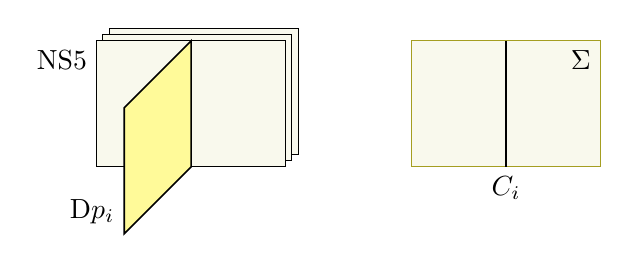
\begin{tikzpicture}[scale=0.8]    %, baseline=(x.base)]        \node (x) at (0,0) {\vphantom{x}};
        
        \filldraw[fill=olive!5, xshift=0.2cm, yshift=0.2cm] (0,0) rectangle (-3,2);
        \filldraw[fill=olive!5, xshift=0.1cm, yshift=0.1cm] (0,0) rectangle (-3,2);
        \filldraw[fill=olive!5] (0,0) rectangle (-3,2) node[below left] {\normalsize NS5};
        
        \filldraw[semithick, fill=yellow!40,] (-1.5,0) -- ++(0,2) -- ++(225:1.5) -- ++(0,-2) node[above left] {\normalsize D$p_{i}$} -- cycle;
        
        \filldraw[color=olive!80, fill=olive!5] (2,0) rectangle (5,2) node[color=black, below left] {\normalsize $\Sigma$};
        \draw[semithick] (3.5,0) node[below] {\normalsize $C_i$} -- ++(0,2);
        
    \end{tikzpicture}
    
  \caption{The D$p$-brane D$p_i$ ending on the NS5-branes creates a defect $\mathcal{E}_{\rm{D}p_i}$ along $C_i$.}
  \label{fig:Dp_on_NS5}
\end{figure}


The low-energy dynamics of the NS5-branes is governed by a six-dimensional
theory $\mathsf{T}_{\mathrm{NS5}}$ on $\mathbb{R}^{4}\times\Sigma$.
The theory $\mathsf{T}_{\mathrm{NS5}}$ is depending on whether IIA
or IIB theory we are considering: 
\begin{align*}
  \textrm{IIA : }    &  \textrm{\ensuremath{\mathcal{N}  =  \left(2,0\right)} superconformal QFT of type \ensuremath{A_{N-1}}},  \\
  \textrm{IIB : }    &  \textrm{\ensuremath{\mathcal{N}  =  \left(1,1\right)}   super Yang-Mills theory with gauge group SU\ensuremath{\left(N\right)}}.
\end{align*}
 The theory $\mathsf{T}_{\mathrm{NS5}}$ is formulated on $\mathbb{R}^{4}\times\Sigma$,
with topological twist along $\Sigma$ which breaks half of sixteen
supercharges. In this twisted theory, D$p_{i}$ create $p$-dimensional
defects $\mathcal{E}_{\mathrm{D}p_{i}}$ on $\mathbb{R}^{p-1}\times C_{i}$,
reducing the number of unbroken supercharges to four. From the point
of view of a four-dimensional observer, this brane configuration gives
half-BPS defects $\mathcal{E}_{\mathrm{D}p_{i}}\left[C_{i}\right]$
in an $\mathcal{N}=2$ theory $\mathsf{T}_{\mathrm{NS5}}\left[\Sigma\right]$.
The total system is invariant under a U($1$) R-symmetry originating
from the rotational symmetry on the $\mathbb{R}^{2}$ factor of the
ten-dimensional spacetime.

Let us take a three-manifold $M$ and ($p-2$)-submanifolds $N_{i}$
of $M$, and modify the above construction so that the world-volumes
of the NS5-branes and the D$p$-branes become $S^{1}\times M\times\Sigma$
and $S^{1}\times N_{i}\times\Sigma_{i}$, respectively. At low energies,
we get the same theory $\mathsf{T}_{\mathrm{NS5}}$ formulated on
$S^{1}\times M\times\Sigma$ and defects $\mathcal{E}_{\mathrm{D}p_{i}}$
located on $S^{1}\times N_{i}\times C_{i}$. In general, this modification
completely breaks supersymmetry. For certain choices of $M$ and $N_{i}$,
however, there is a string background in which a fraction of supersymmetry
is still preserved. In such a background, the path integral computes
the \emph{supersymmetric index} of $\mathsf{T}_{\mathrm{NS5}}$, defined
with respect to the Hilbert space on $M\times\Sigma$ in the presence
of defects $\mathcal{E}_{\mathrm{D}p_{i}}$ inserted on $N_{i}\times C_{i}$. 

A salient feature of supersymmetric indices is that they are protected
against continuous changes of various parameters of the theory. This
means that the index of our theory is invariant under deformations
of the geometric data of $\Sigma$ and $C_{i}$, namely the metric
on $\Sigma$ and the shapes of $C_{i}$. In other words, the theory
$\mathsf{T}_{\mathrm{NS5}}$ on $S^{1}\times M\times\Sigma$ is topological
on $\Sigma$, as far as the computation of the index is concerned. 

To relate the present setup to the one considered in the previous
subsection, we apply T-duality along $S^{1}$. It turns D$p_{i}$
into D$\left(p-1\right)$-branes D$\left(p-1\right)_{i}$, localized
at points $u_{i}$ along the dual circle $\tilde{S}^{1}$, while sending
the NS5-branes to those in the other type II string theory. The new
NS5-branes produce the dual six-dimensional theory $\tilde{\mathsf{T}}_{\mathrm{NS5}}$
on $\tilde{S}^{1}\times M\times\Sigma$, and in this theory D$\left(p-1\right)_{i}$
create ($p-1$)-dimensional defects $\mathcal{E}_{\mathrm{D}\left(p-1\right)_{i}}$
on $\left\{ u_{i}\right\} \times N_{i}\times C_{i}$. Thus we are
in the situation studied in the last subsection, and the correlation
function for this configuration coincides with the partition function
of an integrable lattice model: 
\begin{equation}
  \left\langle \prod_{i=1}^{l}\mathcal{E}_{\mathrm{D}p_{i}}\left[C_{i}\right]\left(S^{1}\times N_{i}\right)\right\rangle_{\mathsf{T}_{\mathrm{NS5}}\left[\Sigma\right],S^{1}\times M}
  =Z_{\mathsf{L}\left(\tilde{\mathsf{T}}_{\mathrm{NS5}}\left[\tilde{S}^{1}\times M\right]\right),\left\{ \mathcal{E}_{\mathrm{D}\left(p-1\right)_{i}}\left[\left\{ u_{i}\right\} \times N_{i}\right]\left(C_{i}\right)\right\} }.
\end{equation}
 Here the left-hand side is expressed in the original frame; it implicitly
depends on each spectral parameter $u_{i}$ through the holonomy $\exp\left(2\pi\mathrm{i}u_{i}\right)$
around $S^{1}$ of the gauge field for the flavor symmetry U$(1)_{i}$
supported on D$p_{i}$. The holonomy appears in the index as a refinement
parameter, or \emph{fugacity}, associated with U$(1)_{i}$. 





\subsubsection{Defects as transfer matrices}

Finally, we apply the construction developed in the precious subsections
to the main theme of this paper; integrable lattice models and defects
as transfer matrices. Let us consider $p=5$ case of the brane construction
in the last subsection. To conform with the standard convention, take
S-duality first and we still have D5- and NS5-branes 
\begin{align*}
  N  \,  \mathrm{D5}   &  \quad S^{1}  \times  M  \times  \Sigma,  \\
  \mathrm{NS5}_{i}    &  \quad S^{1}  \times  N_{i}  \times  \Sigma_{i},
\end{align*}
where NS$5_{i}$ create defects $\mathcal{E}_{\mathrm{NS}5_{i}}$
on $S^{1}\times N_{i}\times C_{i}$. 

One should notice that in this setup we necessarily have $N_{i}=M$
and thus the defects $\mathcal{E}_{\mathrm{NS}5_{i}}$ fill the whole
$S^{1}\times M$, which produces a four-dimensional theory 
\[
\mathsf{T}_{\mathrm{D5NS5}}\left[\Sigma\right]
\]
with $\mathcal{N}=1$ supersymmetry. Then we now have 
\begin{equation}
  \left\langle  1  \right\rangle_{\mathsf{T}_{\mathrm{D5NS5}}\left[\Sigma\right], S^{1}\times M}  
    =Z_{\mathsf{L}\left(\mathsf{T}_{\mathrm{D5NS5}}\left[S^{1}\times M\right]\right),\left\{ \mathcal{E}_{i}\left[S^{1}\times M\right]\left(C_{i}\right)\right\} }.
\end{equation}
For example, when $M=S^{3}$, the left-hand side is given by the supersymmetric
index for $\mathcal{N}=1$ theory and the right-hand side corresponds
to the partition function of Bazhanov-Sergeev integrable lattice model
\cite{Bazhanov:2010kz,Bazhanov:2011mz,Spiridonov:2010em,Yamazaki:2012cp}. When $M=L\left(p,1\right)$,
lens space, the left-hand side is computed in \cite{Yamazaki:2013nra}, which
defines a new integrable lattice model through this correspondence. 

The brane tiling construction of integrable lattice models can be
enriched by introduction of additional defects. Besides the previously
defined D5NS5-brane system, introduce a D3-brane such as 
\begin{align}
  \mathrm{D3}    &  \quad S^{1}  \times  N  \times  C  \times  \mathbb{R}_{+},\\
  \mathrm{D3'}   &  \quad S^{1}  \times\left\{ 0\right\}  \times  C'  \times  \mathbb{R}^{2},
\end{align}
 where $N$ is a curve in $M$ and $C,\,C'$ are 1-cycles on $\Sigma$.
A single D3-brane insertion corresponds to a new oriented line in
the integrable lattice model, which we represent by a dashed line.
Now that we have two kinds of lines, we can define three R-matrices:
\begin{equation}
  R=
    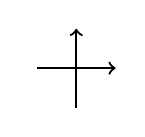
\begin{tikzpicture}[scale=0.5, baseline=(x.base)]
        \node (x) at (0,0) {\vphantom{x}};
        
        \draw[thick, ->] (0,0) -- (2,0);
        \draw[thick, ->] (1,-1) -- (1,1);
        
    \end{tikzpicture}
  \, ,
  \quad
  L=
    \begin{tikzpicture}[scale=0.5, baseline=(x.base)]
        \node (x) at (0,0) {\vphantom{x}};
        
        \draw[thick, densely dashed, ->] (0,0) -- (2,0);
        \draw[thick, ->] (1,-1) -- (1,1);
        
    \end{tikzpicture}
  \, ,
  \quad
  \mathcal{R}=
    \begin{tikzpicture}[scale=0.5, baseline=(x.base)]
        \node (x) at (0,0) {\vphantom{x}};
        
        \draw[thick, densely dashed, ->] (0,0) -- (2,0);
        \draw[thick, densely dashed, ->] (1,-1) -- (1,1);
        
    \end{tikzpicture}
  \, .
\end{equation}
 The middle one is usually called \emph{L-operator}. Correspondingly,
we have four Yang-Baxter equations, involving zero to three dashed
lines. Those that involving one or two dashed line, 
\begin{equation}
    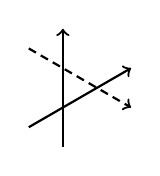
\begin{tikzpicture}[scale=0.5, baseline=(x.base)]
        \node (x) at (30:2) {};
        
        \draw[thick, ->] (0,0) -- ++(30:3);
        \draw[thick, densely dashed, ->] (0,2) -- ++(-30:3);
        \draw[thick, ->] (-30:1) -- ++(0,3);
        
    \end{tikzpicture}
  \ = 
    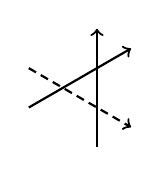
\begin{tikzpicture}[scale=0.5, baseline=(x.base)]
        \node (x) at (30:1) {};
        
        \draw[thick, ->] (0,0) -- ++(30:3);
        \draw[thick, densely dashed, ->] (0,1) -- ++(-30:3);
        \draw[thick, ->] (-30:2) -- ++(0,3);
        
    \end{tikzpicture}
%
  \quad  \text{and}  \quad
%
    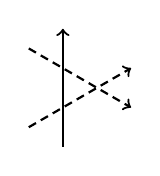
\begin{tikzpicture}[scale=0.5, baseline=(x.base)]
        \node (x) at (30:2) {};
        
        \draw[thick, densely dashed, ->] (0,0) -- ++(30:3);
        \draw[thick, densely dashed, ->] (0,2) -- ++(-30:3);
        \draw[thick, ->] (-30:1) -- ++(0,3);
        
    \end{tikzpicture}
  \ = 
    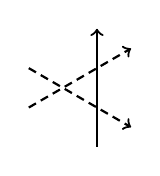
\begin{tikzpicture}[scale=0.5, , baseline=(x.base)]
        \node (x) at (30:1) {};
        
        \draw[thick, densely dashed, ->] (0,0) -- ++(30:3);
        \draw[thick, densely dashed, ->] (0,1) -- ++(-30:3);
        \draw[thick, ->] (-30:2) -- ++(0,3);
        
    \end{tikzpicture}
\end{equation}
 are called \emph{RLL relations}. The effect of the insertion of such
an additional defect on the lattice model is seen in terms of the
L-operator. The neighborhood of the dashed line looks like 
\begin{equation}
    \begin{tikzpicture}[scale=0.9, baseline=(x.base)]
        \node (x) at (0,0) {\vphantom{x}};
        
        \draw[thick, ->] (0.3,-0.4) -- (0.3, 0.6);
        \draw[thick, ->] (0.9,-0.4) -- (0.9, 0.6);
        \draw[thick, ->] (2.7,-0.4) -- (2.7, 0.6);
        
        \draw[thick] (0,0.2) to[out=180, in=180] (0,0);
        \draw[thick, ->-=0.24, densely dashed] (0,0) -- (3,0);
        \draw[thick] (3,0) to[out=0, in=0] (3,0.2); 
        
        \draw[preaction={draw=white, ultra thick}, thick, loosely dotted] (1.4,0) -- (2.1,0);
    
    \end{tikzpicture}
    \quad . 
\end{equation}
This diagram shows that the defect acts on the lattice model by a
transfer matrix constructed from L-operators. Thus, the insertion
of a defect operator in four-dimensional theory is mapped into lattice
model side as the action of a transfer matrix constructed from L-operators. 

What we would like to discuss in detail in the subsequent sections
are the introduction of a single D3-brane (equation of D3D3') to the
D5NS5-brane system, and clarify that the correspondence with the additional
defects. In the next two sections, we are considering the followings: 
\begin{enumerate}
	\item For the case of single D3, let $M=S^{3}$, $\Sigma=T^{2}$, and $N=S^{1}$.
Then the D3 creates a surface defect on $S^{1}\times S^{1}$ and it
acts on supersymmetric index as a transfer matrix in the corresponding
lattice model: 
\begin{align}
  \left\langle  1  \right\rangle_{\mathsf{T}_{\mathrm{D5NS5}}\left[\Sigma\right],S^{1}\times S^{3}}  
    &  =  \mathcal{I}_{S^{1}\times S^{3}}\left(p,q,t\right),\\
  Z_{\mathsf{L}\left(\mathsf{T}_{\mathrm{D5NS5}}\left[S^{1}\times S^{3}\right]\right),\left\{ \mathcal{E}_{i}\left[S^{1}\times S^{3}\right]\left(C_{i}\right)\right\} }  
    &  =  Z_{\mathrm{Bazhanov-Sergeev}},
\end{align}
 the surface defect index is represented as a difference operator
acting on the original supersymmetric index \cite{Gaiotto:2012xa,Gadde:2013dda}, 
\begin{equation}
  \left\langle S_{\left(r,s\right)}\right\rangle_{\mathsf{T}_{\mathrm{D5NS5}}\left[\Sigma\right]}  
  =  \mathfrak{S}_{\left(r,s\right)}\mathcal{I}_{S^{1}\times S^{3}}\left(p,q,t\right).
\end{equation}
\item For the case of single D3', let $M=\mathbb{R}^{3}$ and $\Sigma=T^{2}$.
D3' creates a line defect wrapping $S^{1}$ and it acts on quantum
Hilbert space of a spin chain as a transfer matrix, since now we have
non-compact three-manifold $\mathbb{R}^{3}$. The line defect in the
four-dimensional theory is realized as a Wilson-'t Hooft line operator
$T$, and its magnetic and electric charge $\left(\mathbf{m},\mathbf{e}\right)$
is specified by the one-cycle C' wrapping the torus $T^{2}$. As it
turns out, the vacuum expectation values (vevs) of Wilson-'t Hooft
lines realize the deformation quantization of the Hitchin moduli space,
and are naturally quantized by the Weyl quantization: 
\begin{equation}
  \textrm{Weyl quantization of }  \left\langle  T_{\left(\mathbf{m},\mathbf{e}\right)}  \right\rangle  
  =  \textrm{trigonometric transfer matrix.}
\end{equation}
\end{enumerate}
%







%\subsection{xxx}









%%%%%%%%%%%%%%%%%%%%%%%%%%%%%%%%%%%%%%%%%%%%%%%%%%%%%%%%%



\bibliographystyle{Common/utphys}
%\nocite{*}
\bibliography{Common/Ref}



\end{document}
\begin{comment}
\documentclass[11pt]{article}  % , titlepage
\usepackage{Common/toshi}
\begin{document}
\end{comment}


%%%%%%%%%%%%%%%%%%%%%%%%%%%%%%%%%%%%%%%%%%%%%%%%%%


\newcommand{\fundbox}{\tikz{\node[fnode, semithick, minimum size=8pt] {}}}


%%%%%%%%%%%%%%%%%% section 4 %%%%%%%%%%%%%%%%%%%%%%%%%%%%%%%%%
\section{Surface defects as transfer matrices}


In this section, we mainly review the results in \cite{Maruyoshi:2016caf},
in which the correspondence we introduce in the previous section was established.


In this section, we apply the general construction of integrable lattice
models from branes in string theory to the simplest case of the so-called
class $\mathcal{S}$ theories. Taking the four-manifold to be $S^{1} \times S^{3}$,
on which quiver gauge theories are defined, the path integral of the
twisted partition function of the theory computes the supersymmetric
index. We first explain the correspondence between the supersymmetric
index and the partition function of two-dimensional integrable lattice
model. Then we proceed to the additional surface defects in the gauge
theory side. The surface defects act on the supersymmetric index by
difference operators, and they are identified with the transfer matrices
of the corresponding integrable lattice model.





\subsection{Brane tilings and integrable lattice models}

In order to give the general argument of the correspondence, let me
briefly review the systematic brane construction of quiver gauge theories
called \emph{brane tilings}. For more details, the reader should be
referred to the original papers and the excellent reviews \cite{Hanany:2005ve,Franco:2005rj,Kennaway:2007tq,Yamazaki:2008bt}. Recall the 5-brane configuration given
in the last part of the previous section (equation of D5NS5),
\begin{align*}
    N\,\mathrm{D5}    & \quad S^{1} \times M \times \Sigma,  \\
    \mathrm{NS5}_{i} & \quad S^{1} \times N_{i} \times \Sigma_{i}.
\end{align*}
For such a configuration, what one needs to notice is that when an
NS5-brane meets $N$ D5-branes, they combine to form a bound state.
In the language of $\left( p,q \right)$ 5-branes, this bound state
is either an $\left( N,1 \right)$ or $\left( N,-1 \right)$ 5-brane,
depending on the relative positions of the branes; see figure \ref{fig:D5NS5config}. Therefore,
the extended defects $\mathcal{E}_{\mathrm{NS5}_{i}}$ are domain
walls in $\mathsf{T}_{\mathrm{D5}}$ separate the spacetime into the
regions with different values of the NS5-brane charge $q$. The curves
$C_{i}$ along which these domain walls are located are known as \emph{zig-zag
paths}. Across a zig-zag path the charge $q$ jump by one.


%FIGURE
\begin{figure}
\centering
  \subfloat[\label{fig:(N,1)}]{

    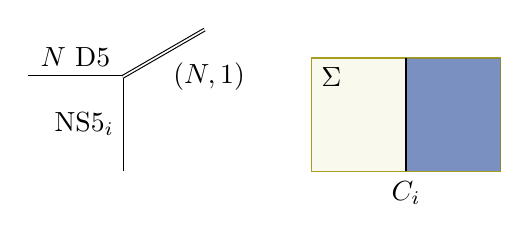
\begin{tikzpicture}[scale=1.2] %, baseline=(x.base)]    \node (x) at (0,0) {\vphantom{x}};

        \draw[xshift=0.01cm] (0,0) -- node[left] {NS5$_i$} ++(0,1);% -- ++(30:1);
        \draw[yshift=0.01cm] (-1,1) -- node[above] {$N$ D5} ++(1,0);% -- ++(30:1);
        \draw[double] (0,1) -- node[below right] {$(N,1)$} ++(30:1);

        \filldraw[color=olive!80, fill=olive!5] (2,1.2) node[color=black, below right] {$\Sigma$} rectangle (4,0);
        \filldraw[color=olive!80, fill=cyan!20!blue, opacity=0.6] (3,0) rectangle (4,1.2);
        \draw[semithick] (3,0) node[below] {$C_i$} -- ++(0,1.2);

    \end{tikzpicture}
    }
  \qquad\qquad
  \subfloat[\label{fig:(N,-1)}]{

    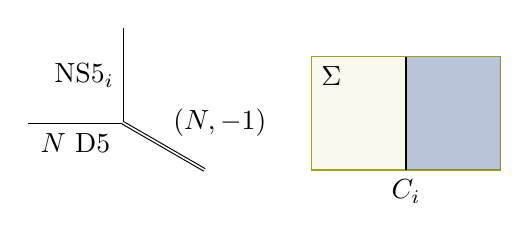
\begin{tikzpicture}[scale=1.2] %, baseline=(x.base)]    \node (x) at (0,0) {\vphantom{x}};
        \def\shift{0.5cm}
        \draw[xshift=0.01cm, yshift=\shift] (0,0) -- node[left] {NS5$_i$} ++(0,1);% -- ++(30:1);
        \draw[yshift=-0.01cm+\shift] (-1,0) -- node[below] {$N$ D5} ++(1,0);% -- ++(30:1);
        \draw[double,yshift=\shift] (0,0) -- node[above right] {$(N,-1)$} ++(-30:1);

        \filldraw[color=olive!80, fill=olive!5] (2,1.2) node[color=black, below right] {$\Sigma$} rectangle (4,0);
        \filldraw[color=olive!80, fill=cyan!20!blue, opacity=0.3] (3,0) rectangle (4,1.2);
        \draw[semithick] (3,0) node[below] {$C_i$} -- ++(0,1.2);

    \end{tikzpicture}
    }
  \caption{An NS5-brane combines with a stack of $N$ D5-branes, forming (a) and $(N,1)$ 5-brane
  or (b) an $(N,-1)$ 5-brane. The 5-brane junction is a domain wall in $\mathsf{T}_{\mathrm{D5}}$.
  The shaded regions shown above support a nonzero NS5-brane charge $q=\pm 1$}
  \label{fig:D5NS5config}
\end{figure}


Conversely, given a configuration of curves $C_{i}$ on the two-dimensional
surface $\Sigma$ and a 5-brane charge assignment consistent with
it, we can construct a 5-brane system whose zig-zag paths are $C_{i}$:
we take NS5-branes approaching the D5-branes from transverse directions,
and let them meet along $C_{i}$ and form bound states over regions
with $q \neq 0$. Such a 5-brane system is called a brane tiling on
$\Sigma$ \cite{Hanany:2005ve,Franco:2005rj}.

As we just explained, a brane tiling gives rise to a four-dimensional
$\mathcal{N}=1$ theory. A concrete description of this theory is
known for the subset of brane tilings that involve only $\left( N,0 \right)$
5-branes (i.e. $N$ coincident D5-branes) and $\left( N,\pm1 \right)$
5-branes. Given a brane tiling in this subset, we indicate $\left( N,1 \right)$
and $\left( N,-1 \right)$ 5-brane regions by dark and light shading,
respectively, while leaving $\left( N,0 \right)$ regions unshaded.
After the shading, we get a checkerboard-like pattern on $\Sigma$
where shaded faces adjoin unshaded ones and two shaded faces sharing
a vertex are of different types, see figure.


%FIGURE    to be fixed
\begin{figure}
\centering
\def\width{3cm}
\def\height{2cm}
  \subfloat[\label{}]{
    \begin{tikzpicture}[scale=1] %, baseline=(x.base)]    \node (x) at (0,0) {\vphantom{x}};
        \def\step{0.15cm}
        \def\shift{0.25cm}
        \def\sep{1cm}

        \fill[fill=olive!5] (0,0) rectangle (\width,\height);

        \fill[lightshade] (0,0) rectangle (\step,\step);
        \fill[lightshade] (\step+\shift,0) rectangle (\step+\sep,\step);    % ????
        \fill[lightshade] (\step+\shift+\sep,0) rectangle (\step+2*\sep,\step);    % ????
        \fill[lightshade] (\step+\shift+2*\sep,0) rectangle (\width,\step);    % ????

        \fill[lightshade] (0,\step+\shift) rectangle (\step,\step+\sep);
        \fill[lightshade] (\step+\shift,\step+\shift) rectangle (\step+\sep,\step+\sep);
        \fill[lightshade] (\step+\shift+\sep,\step+\shift) rectangle (\step+2*\sep,\step+\sep);
        \fill[lightshade] (\step+\shift+2*\sep,\step+\shift) rectangle (\width,\step+\sep);

        \fill[lightshade] (0,\step+\shift+\sep) rectangle (\step,\height);
        \fill[lightshade] (\step+\shift,\step+\shift+\sep) rectangle (\step+\sep,\height);
        \fill[lightshade] (\step+\shift+\sep,\step+\shift+\sep) rectangle (\step+2*\sep,\height);
        \fill[lightshade] (\step+\shift+2*\sep,\step+\shift+\sep) rectangle (\width,\height);

        \fill[darkshade] (\step,\step) rectangle (\step+\shift,\step+\shift);
        \fill[darkshade, xshift=\sep] (\step,\step) rectangle (\step+\shift,\step+\shift);
        \fill[darkshade, xshift=2*\sep] (\step,\step) rectangle (\step+\shift,\step+\shift);

        \begin{scope}[yshift=\sep]
        \fill[darkshade] (\step,\step) rectangle (\step+\shift,\step+\shift);
        \fill[darkshade, xshift=\sep] (\step,\step) rectangle (\step+\shift,\step+\shift);
        \fill[darkshade, xshift=2*\sep] (\step,\step) rectangle (\step+\shift,\step+\shift);
        \end{scope}

        \draw[semithick] (\step,0) -- ++(0,\height);
        \draw[semithick, xshift=\shift] (\step,0) -- ++(0,\height);
        \draw[semithick, xshift=\sep] (\step,0) -- ++(0,\height);
        \draw[semithick, xshift=\sep+\shift] (\step,0) -- ++(0,\height);
        \draw[semithick, xshift=2*\sep] (\step,0) -- ++(0,\height);
        \draw[semithick, xshift=2*\sep+\shift] (\step,0) -- ++(0,\height);

        \draw[semithick] (0,\step) -- ++(\width,0);
        \draw[semithick, yshift=\shift] (0,\step) -- ++(\width,0);
        \draw[semithick, yshift=\sep] (0,\step) -- ++(\width,0);
        \draw[semithick, yshift=\sep+\shift] (0,\step) -- ++(\width,0);

        \draw[color=olive!80] (0,0) rectangle (\width,\height);


    \end{tikzpicture}
    }
  \quad
  \subfloat[\label{}]{
    \begin{tikzpicture}[scale=1] %, baseline=(x.base)]    \node (x) at (0,0) {\vphantom{x}};
        \useasboundingbox (0,0) rectangle (\width,\height);

        \def\step{0.15cm}
        \def\shift{0.25cm}
        \def\sep{1cm}
        \def\site{\shift+\sep/2}

        \node[node, minimum size=7pt] (a1) at (\site,\step+\shift/2) {};  %%%%
        \node[node, minimum size=7pt, xshift=\sep] (a2) at (\site,\step+\shift/2) {};
        \node[node, minimum size=7pt, xshift=2*\sep] (a3) at (\site,\step+\shift/2) {};
        \node[node, minimum size=7pt] (b1) at (\step+\shift/2,\site) {};  %%%%
        \node[node, minimum size=7pt, xshift=\sep] (b2) at (\step+\shift/2,\site) {};
        \node[node, minimum size=7pt, xshift=2*\sep] (b3) at (\step+\shift/2,\site) {};
        \begin{scope}[yshift=\sep]
        \node[node, minimum size=7pt] (c1) at (\site,\step+\shift/2) {};  %%%%
        \node[node, minimum size=7pt, xshift=\sep] (c2) at (\site,\step+\shift/2) {};
        \node[node, minimum size=7pt, xshift=2*\sep] (c3) at (\site,\step+\shift/2) {};
        \node[node, minimum size=7pt] (d1) at (\step+\shift/2,\site) {};  %%%%
        \node[node, minimum size=7pt, xshift=\sep] (d2) at (\step+\shift/2,\site) {};
        \node[node, minimum size=7pt, xshift=2*\sep] (d3) at (\step+\shift/2,\site) {};
        \end{scope}

        \draw[semithick, arrows=-latex] (b1) to (a1); \draw[semithick, arrows=-latex] (a1) to (b2); \draw[semithick, arrows=-latex] (b2) to (a2); \draw[semithick, arrows=-latex] (a2) to (b3); \draw[semithick, arrows=-latex] (b3) to (a3);
        \draw[semithick, arrows=-latex] (c1) to (b1); \draw[semithick, arrows=-latex] (b2) to (c1); \draw[semithick, arrows=-latex] (c2) to (b2); \draw[semithick, arrows=-latex] (b3) to (c2); \draw[semithick, arrows=-latex] (c3) to (b3);
        \draw[semithick, arrows=-latex] (d1) to (c1); \draw[semithick, arrows=-latex] (c1) to (d2); \draw[semithick, arrows=-latex] (d2) to (c2); \draw[semithick, arrows=-latex] (c2) to (d3); \draw[semithick, arrows=-latex] (d3) to (c3);

        \path[name path=rec, draw=none] (0,0) rectangle (\width,\height);
        \path[name path=quiv1, draw=none] (a1) to (\step+\shift/2,\site-\sep);
        \path[name path=quiv2, draw=none] (a1) to (\step+\shift/2+\sep,\site-\sep);
        \path[name intersections={of= rec and quiv1, by={A}}];\tikzmath{coordinate \a;  \a = (A);}    % actually \ay=0!!
        \path[name intersections={of= rec and quiv2, by={B}}];\tikzmath{coordinate \b;  \b = (B);}    % actually \by=0!!

        \draw[semithick] (\ax,0) to (a1); \draw[semithick, arrows=-latex] (\bx,0) to (a1);
        \draw[semithick] (\ax+\sep,0) to (a2); \draw[semithick, arrows=-latex] (\bx+\sep,0) to (a2);
        \draw[semithick] (\ax+2*\sep,0) to (a3); \draw[semithick, arrows=-latex] (\width,0) to (a3);  %\bx+2*\sep

        \draw[semithick, arrows=-latex] (0,\ax) to (b1); \draw[semithick] (0,\bx) to (b1);
        \draw[semithick, arrows=-latex] (0,\ax+\sep) to (d1);

        \draw[semithick] (\width-\bx,\height) to (d3); \draw[semithick, arrows=-latex] (\width-\ax,\height) to (d3);
        \draw[semithick] (\width-\bx-\sep,\height) to (d2); \draw[semithick, arrows=-latex] (\width-\ax-\sep,\height) to (d2);
        \draw[semithick] (0,\height) to (d1); \draw[semithick, arrows=-latex] (\width-\ax-2*\sep,\height) to (d1);

        \draw[semithick] (\width,\height-\ax) to (c3); \draw[semithick, arrows=-latex] (\width,\height-\bx) to (c3);
        \draw[semithick] (\width,\height-\ax-\sep) to (a3);

        \draw[color=olive!80] (0,0) rectangle (\width,\height);

    \end{tikzpicture}
    }
  \quad
  \subfloat[\label{}]{
      \begin{tikzpicture}[scale=1] %, baseline=(x.base)]    \node (x) at (0,0) {\vphantom{x}};
        \def\step{0.15cm}
        \def\shift{0.25cm}
        \def\sep{1cm}

        \path[name path=v1, draw=none] (\step+\sep/2,0) -- ++(0,\height);
        \path[name path=l1, draw=none] (\step+\sep/2-\shift,0) -- ++(\height,\height);    % canonical line
        \path[name intersections={of= v1 and l1, by={A}}];\tikzmath{coordinate \ca;  \ca = (A);}

        \fill[fill=olive!5] (0,0) rectangle (\width,\height);

        \fill[darkshade] (\step+\sep/2-\shift,0) -- (\step+\sep/2,0) -- (\cax,\cay) -- cycle;
        \fill[lightshade] (\step+\sep/2,\step+\sep/2) -- (\cax,\cay) -- (\step+\sep/2-\shift+\cax,\step+\sep/2) -- cycle;
        \fill[darkshade] (\step+\sep/2,\step+\sep/2) -- (\cax,\cay+\sep) -- (0,\step+\sep/2) -- cycle;
        \fill[lightshade, yshift=\sep] (\step+\sep/2,\step+\sep/2) -- (\cax,\cay) -- (\step+\sep/2-\shift+\cax,\step+\sep/2) -- cycle;
        \fill[darkshade] (0,\step+\sep/2+\sep) -- (\step+\sep/2,\step+\sep/2+\sep) -- (\step+\sep/2,\height) -- (\step+\sep/2-\shift,\height) -- cycle;

        \begin{scope}[xshift=\sep]
        \fill[darkshade] (\step+\sep/2-\shift,0) -- (\step+\sep/2,0) -- (\cax,\cay) -- cycle;
        \fill[lightshade] (\step+\sep/2,\step+\sep/2) -- (\cax,\cay) -- (\step+\sep/2-\shift+\cax,\step+\sep/2) -- cycle;
        \fill[darkshade] (\step+\sep/2,\step+\sep/2) -- (\cax,\cay+\sep) -- (0,\step+\sep/2) -- cycle;
        \fill[lightshade, yshift=\sep] (\step+\sep/2,\step+\sep/2) -- (\cax,\cay) -- (\step+\sep/2-\shift+\cax,\step+\sep/2) -- cycle;
        \fill[darkshade] (0,\step+\sep/2+\sep) -- (\step+\sep/2,\step+\sep/2+\sep) -- (\step+\sep/2,\height) -- (\step+\sep/2-\shift,\height) -- cycle;
        \end{scope}

        \begin{scope}[xshift=2*\sep]
        \fill[darkshade] (\step+\sep/2-\shift,0) -- (\step+\sep/2,0) -- (\cax,\cay) -- cycle;
        \fill[lightshade] (\step+\sep/2,\step+\sep/2) -- (\cax,\cay) -- (\step+\sep/2-\shift+\cax,\step+\sep/2) -- cycle;
        \fill[darkshade] (\step+\sep/2,\step+\sep/2) -- (\cax,\cay+\sep) -- (0,\step+\sep/2) -- cycle;
        \fill[lightshade, yshift=\sep] (\step+\sep/2,\step+\sep/2) -- (\cax,\cay) -- (\step+\sep/2-\shift+\cax,\step+\sep/2) -- cycle;
        \fill[darkshade] (0,\step+\sep/2+\sep) -- (\step+\sep/2,\step+\sep/2+\sep) -- (\step+\sep/2,\height) -- (\step+\sep/2-\shift,\height) -- cycle;
        \end{scope}

        % vertical lines
        \draw[semithick] (\step+\sep/2,0) -- ++(0,\height);
        \draw[semithick, xshift=\sep] (\step+\sep/2,0) -- ++(0,\height);
        \draw[semithick, xshift=2*\sep] (\step+\sep/2,0) -- ++(0,\height);

        % horizontal lines
        \draw[semithick] (0,\step+\sep/2) -- ++(\width,0);
        \draw[semithick, yshift=\sep] (0,\step+\sep/2) -- ++(\width,0);

        \draw[semithick] (0,\step+\sep/2+\sep) -- (\step+\sep/2-\shift,\height);
        \draw[semithick] (0,\step+\sep/2) -- (\step+\sep/2+\sep-\shift,\height);
        \draw[semithick] (\step+\sep/2-\shift,0) -- ++(\height,\height);    % canonical line
        \draw[semithick] (\step+\sep/2-\shift+\sep,0) -- (\width,\step+\sep/2+\sep);
        \draw[semithick] (\step+\sep/2-\shift+2*\sep,0) -- (\width,\step+\sep/2);

        \draw[color=olive!80] (0,0) rectangle (\width,\height);

    \end{tikzpicture}
  }
  \quad
  \subfloat[\label{}]{
    \begin{tikzpicture}[scale=1] %, baseline=(x.base)]    \node (x) at (0,0) {\vphantom{x}};
        \useasboundingbox (0,0) rectangle (\width,\height);

        \def\step{0.15cm}
        \def\shift{0.25cm}
        \def\sep{1cm}
        \def\site{2*\step}

        \node[fnode, minimum size=7pt] (a1) at (1.2*\site,\site) {};
        \node[fnode, minimum size=7pt, xshift=\sep] (a2) at (1.2*\site,\site) {};
        \node[fnode, minimum size=7pt, xshift=2*\sep] (a3) at (1.2*\site,\site) {};

        \begin{scope}[yshift=0.7*\sep]
        \node[node, minimum size=7pt] (b1) at (1.2*\site,\site) {};
        \node[node, minimum size=7pt, xshift=\sep] (b2) at (1.2*\site,\site) {};
        \node[node, minimum size=7pt, xshift=2*\sep] (b3) at (1.2*\site,\site) {};
        \end{scope}

        \begin{scope}[yshift=1.4*\sep]
        \node[fnode, minimum size=7pt] (c1) at (1.2*\site,\site) {};
        \node[fnode, minimum size=7pt, xshift=\sep] (c2) at (1.2*\site,\site) {};
        \node[fnode, minimum size=7pt, xshift=2*\sep] (c3) at (1.2*\site,\site) {};
        \end{scope}

        \draw[semithick, -latex] (a1) to (a2); \draw[semithick, -latex] (a2) to (a3);
        \draw[semithick, -latex] (a1) to (b1); \draw[semithick, -latex] (a2) to (b2); \draw[semithick, -latex] (a3) to (b3);
        \draw[semithick, -latex] (b1) to (b2); \draw[semithick, -latex] (b2) to (b3);
        \draw[semithick, -latex] (b1) to (c1); \draw[semithick, -latex] (b2) to (c2); \draw[semithick, -latex] (b3) to (c3);
        \draw[semithick, -latex] (b2) to (a1); \draw[semithick, -latex] (b3) to (a2);
        \draw[semithick, -latex] (c2) to (b1); \draw[semithick, -latex] (c3) to (b2);


        \path[name path=rec, draw=none] (0,0) rectangle (\width,\height);
        \path[name path=quiv, draw=none] (b1) to (\site-\sep,\site);
        \path[name intersections={of= rec and quiv, by={A}}];\tikzmath{coordinate \ca;  \ca = (A);}    % actually \cax=0!!

        \draw[semithick] (b1) to (\cax,\cay); \draw[semithick] (c1) to (\cax,\cay+0.7*\sep);
        \draw[semithick, -latex] (0,\site) to (a1); \draw[semithick, -latex] (0,\site+0.7*\sep) to (b1);

        \draw[semithick, -latex] (\width,\cay) to (a3); \draw[semithick, -latex] (\width,\cay+0.7*\sep) to (b3);
        \draw[semithick] (a3) to (\width,\site); \draw[semithick] (b3) to (\width,\site+0.7*\sep);

        \draw[color=olive!80] (0,0) rectangle (\width,\height);

    \end{tikzpicture}
    }
  \caption{(a) A brane tiling on a torus. (b) The periodic quiver associated with (a).
  (c) A brane tiling on a finite-length cylinder. (d) the quiver for (c).}
  \label{fig:tilings_quiverdiagram}
\end{figure}


Each unshaded region supports $N$ D5-branes, hence an $\SU(N)$ vector
multiplet lives there. If the region contains part of the boundary,
the multiplet is frozen by boundary conditions and the associated
symmetry is an $\SU(N)$ flavor symmetry; in quiver notation, we represent
a dynamical vector multiplet by a gauge node (circle) and a non-dynamical
one by a flavor node (square). From open strings stretched between
two unshaded regions (namely ending on $N$ D5-branes partitioned
by NS5-brane) sharing a vertex, we get a chiral multiplet that transforms
in the fundamental representation under one of the associated gauge
or flavor groups and in the anti-fundamental representation under
the other. We write it by an arrow between the two nodes:
\begin{equation}
    \begin{tikzpicture}[scale=1.2, baseline=(x.base)]    \node (x) at (0,0) {\vphantom{x}};

        \fill[color=olive!5] (-0.5,-0.5) rectangle (0.5,0.5);
        \fill[darkshade] (0.5,-0.5) -- (0.5,0.5) -- (0,0) -- cycle;
        \fill[lightshade] (-0.5,0.5) -- (-0.5,-0.5) -- (0,0) -- cycle;

        \draw (-0.5,-0.5) node[below] {$i$} -- ++(45:{sqrt(2)});
        \draw (0.5,-0.5) node[below] {$j$} -- ++(135:{sqrt(2)});

    \end{tikzpicture}
  %
  \quad  \rightsquigarrow  \quad
  %
    \begin{tikzpicture}[scale=1, baseline=(x.base)]    \node (x) at (0,0) {\vphantom{x}};

        \node[fnode] (a) at (0,-0.5) {};
        \node[fnode] (b) at (0,0.5) {};
        \draw[semithick, arrows=-latex] (a) to (b);

    \end{tikzpicture}
  \quad .
  \label{eq:bifund}
\end{equation}
 The arrow points from the anti-fundamental side to the fundamental
side. See figure \ref{fig:tilings_quiverdiagram} for examples of quivers obtained from brane tilings.

Moreover, for every set of zig-zag paths bounding a shaded region,
we have a loop of arrows and world-sheet instantons generate a superpotential
term given by the trace of the product of the bifundamental chiral
multiplets in the loop. The coefficient of this term is positive or
negative depending on whether the direction of the loop is clockwise
or counterclockwise. Thus, the four-dimensional theory realized by
a brane tiling in the subset under consideration is an $\mathcal{N}=1$
supersymmetric gauge theory described by a quiver with potential drawn
on $\Sigma$.

Each NS5$_{i}$ supports a $\U(1)$ flavor symmetry $\U(1)_{i}$. An
arrow is charged under $\U(1)_{i}$ if it is crossed by $C_{i}$. The
charge $F_{i}$ of $\U(1)_{i}$ can be normalized in such a way that
the arrow in (\ref{eq:bifund}) has $F_{i}=-1$ and $F_{j}=+1$. The
diagonal combination of all $\U(1)_{i}$ acts on the theory trivially
since every arrow is crossed by exactly two zig-zag paths from the
opposite sides.

The theory also has an R-symmetry $\U(1)_{R}$. Its definition is not
unique as the R-charge $R$ can be shifted by a linear combination
of $\U(1$) flavor charges. However, the R-charge assignment is constrained
by two conditions. The first is that $\U(1)_{R}$ must be unbroken
by the superpotential and therefore the R-charges of the chiral multiplets
contained in each superpotential term must add up to two. The second
is that $\U(1)_{R}$ must be free of anomaly. This requires that for
every gauge node, the sum of the R-charges of the arrows starting
from or ending at that node must equal the number of the arrows minus
two.

To fix the R-charge assignment, let us assume that we can orient the
zig-zag paths and bound every shaded or unshaded region with zig-zag
paths all heading upward, for some choice of the ``vertical'' direction
in the neighborhood of that region. This is the case for the examples
in figure \ref{fig:tilings_quiverdiagram}. The zig-zag paths thus oriented fall into two groups; when
a zig-zag path goes upward and we cross it from the left to the right,
$q$ increases by one. We distinguish the latter case from the former
by drawing the zig-zag path with a dotted line. Then, we give an arrow
$R=0$ if it originates from a crossing of two zig-zag paths of the
same type, and $R=1$ otherwise. With this R-charge assignment the
two conditions describe above are satisfied (see figure \ref{fig:twoexamples}).


%FIGURE
\begin{figure}
\centering
  \subfloat[\label{}]{
    \begin{tikzpicture}[scale=1] %, baseline=(x.base)]    \node (x) at (0,0) {\vphantom{x}};
        \def\radius{1.2cm}

        \path[name path=dot1, draw=none] (280:\radius) to[bend left=10] (190:\radius);
        \path[name path=dot2, draw=none] (225:\radius) to[bend right=10] (135:\radius);
        \path[name path=dot3, draw=none] (170:\radius) to[bend left=10] (60:\radius);
        \path[name path=solid1, draw=none] (260:\radius) to[bend left=10] (340:\radius);
        \path[name path=solid2, draw=none] (315:\radius) to[bend left=10] (30:\radius);
        \path[name path=solid3, draw=none] (0:\radius) -- (100:\radius);

        \path[name intersections={of= dot1 and solid1, by={A}}];
        \path[name intersections={of= dot1 and dot2, by={B}}];
        \path[name intersections={of= dot2 and dot3, by={C}}];
        \path[name intersections={of= dot3 and solid3, by={D}}];
        \path[name intersections={of= solid2 and solid3, by={E}}];
        \path[name intersections={of= solid1 and solid2, by={F}}];

        \fill[olive!5] (0,0) circle[radius=\radius];

        \fill[darkshade] (A) to (260:\radius) arc (260:280:\radius) -- cycle;
        \fill[darkshade] (B) to (190:\radius) arc (190:225:\radius) -- cycle;
        \fill[darkshade] (C) to (135:\radius) arc (135:170:\radius) -- cycle;
        \fill[darkshade] (D) to (60:\radius) arc (60:100:\radius) -- cycle;
        \fill[darkshade] (E) to (0:\radius) arc (0:30:\radius) -- cycle;
        \fill[darkshade] (F) to (315:\radius) arc (315:340:\radius) -- cycle;

        \fill[lightshade] (A) to[bend left=5] (B) to[bend right=5] (C) to[bend left=5] (D) -- (E) to[bend right=5] (F) to[bend right=5] cycle;

        \draw[semithick, densely dotted, ->] (280:\radius) to[bend left=10] (190:\radius);
        \draw[semithick, densely dotted, ->] (225:\radius) to[bend right=10] (135:\radius);
        \draw[semithick, densely dotted, ->] (170:\radius) to[bend left=10] (60:\radius);
        \draw[semithick, ->] (260:\radius) to[bend left=10] (340:\radius);
        \draw[semithick, ->] (315:\radius) to[bend left=10] (30:\radius);
        \draw[semithick, ->] (0:\radius) -- (100:\radius);

        \begin{scope}[scale=0.8]
        \node[fnode, xshift=2.4*\radius] (a) at (350:\radius) {};\node[fnode, xshift=2.4*\radius] (b) at (45:\radius) {};
        \node[fnode, xshift=2.4*\radius] (c) at (235/2:\radius) {};\node[fnode, xshift=2.4*\radius] (d) at (180:\radius) {};
        \node[fnode, xshift=2.4*\radius] (e) at (485/2:\radius) {};\node[fnode, xshift=2.4*\radius] (f) at (595/2:\radius) {};
        \draw[semithick, arrows=-latex] (a) -- (b);\draw[semithick, arrows=-latex] (b) -- (c);\draw[semithick, arrows=-latex] (c) -- (d);
        \draw[semithick, arrows=-latex] (d) -- (e);\draw[semithick, arrows=-latex] (e) -- (f);\draw[semithick, arrows=-latex] (f) -- (a);
        \end{scope}

    \end{tikzpicture}
    }
  %
  \qquad\qquad
  %
  \subfloat[\label{}]{
    \begin{tikzpicture}[scale=1] %, baseline=(x.base)]    \node (x) at (0,0) {\vphantom{x}};
        \def\radius{1.2cm}

        \path[name path=dot1, draw=none] (280:\radius) to[bend left=10] (190:\radius);
        \path[name path=dot2, draw=none] (225:\radius) to[bend right=10] (135:\radius);
        \path[name path=dot3, draw=none] (170:\radius) to[bend left=10] (60:\radius);
        \path[name path=solid1, draw=none] (260:\radius) to[bend left=10] (340:\radius);
        \path[name path=solid2, draw=none] (315:\radius) to[bend left=10] (30:\radius);
        \path[name path=solid3, draw=none] (0:\radius) -- (100:\radius);

        \path[name intersections={of= dot1 and solid1, by={A}}];
        \path[name intersections={of= dot1 and dot2, by={B}}];
        \path[name intersections={of= dot2 and dot3, by={C}}];
        \path[name intersections={of= dot3 and solid3, by={D}}];
        \path[name intersections={of= solid2 and solid3, by={E}}];
        \path[name intersections={of= solid1 and solid2, by={F}}];

        \fill[olive!5] (0,0) circle[radius=\radius];

        \fill[darkshade] (A) to[bend left=5] (B) to (225:\radius) arc (225:260:\radius) --(A) -- cycle;
        \fill[lightshade] (B) to[bend right=5] (C) to (170:\radius) arc (170:190:\radius) -- (B) -- cycle;
        \fill[darkshade] (C) to[bend left=5] (D) to (100:\radius) arc (100:135:\radius) -- (C) -- cycle;
        \fill[lightshade] (D) to (E) to (30:\radius) arc (30:60:\radius) -- (D) -- cycle;
        \fill[darkshade] (E) to[bend right=5] (F) to (340:\radius) arc (340:360:\radius) -- (E) -- cycle;
        \fill[lightshade] (F) to[bend right=5] (A) to (280:\radius) arc (280:315:\radius) (F) -- cycle;

        %\fill[lightshade] (A) to[bend left=5] (B) to[bend right=5] (C) to[bend left=5] (D) -- (E) to[bend right=5] (F) to[bend right=5] cycle;

        \draw[semithick, densely dotted, ->] (280:\radius) to[bend left=10] (190:\radius);
        \draw[semithick, ->] (225:\radius) to[bend right=10] (135:\radius);
        \draw[semithick, densely dotted, ->] (170:\radius) to[bend left=10] (60:\radius);
        \draw[semithick, densely dotted, ->] (260:\radius) to[bend left=10] (340:\radius);
        \draw[semithick, ->] (315:\radius) to[bend left=10] (30:\radius);
        \draw[semithick, densely dotted, ->] (0:\radius) -- (100:\radius);

        \begin{scope}[scale=0.8]
        \node[fnode, xshift=2.4*\radius] (a) at (15:\radius) {};\node[fnode, xshift=2.4*\radius] (b) at (80:\radius) {};
        \node[fnode, xshift=2.4*\radius] (c) at (305/2:\radius) {};\node[fnode, xshift=2.4*\radius] (d) at (415/2:\radius) {};
        \node[fnode, xshift=2.4*\radius] (e) at (270:\radius) {};\node[fnode, xshift=2.4*\radius] (f) at (655/2:\radius) {};
        \node[node,  xshift=2.4*\radius] (g) at (0,0) {};
        \draw[semithick, arrows=-latex] (g) -- (a);\draw[semithick, arrows=-latex] (b) -- (g);\draw[semithick, arrows=-latex] (g) -- (c);
        \draw[semithick, arrows=-latex] (d) -- (g);\draw[semithick, arrows=-latex] (g) -- (e);\draw[semithick, arrows=-latex] (f) -- (g);
        \end{scope}

    \end{tikzpicture}
    }
  \caption{Zig-zag paths bounding (a) a shaded region and (b) an unshaded region.
  In either case, the R-charges of two of the arrows are different from those of the rest.}
  \label{fig:twoexamples}
\end{figure}


Summarizing the rules for assignment of the charges, we can read off
the quiver diagram from zig-zag paths as in figure \ref{fig:rule_for_quiver}.

%FIGURE
\begin{figure}
\centering
\newcommand{\shift}{1.3cm}
  \subfloat[\label{}]{
        \begin{tikzpicture}[scale=1.2, baseline=(x.base)]    \node (x) at (0,0) {\vphantom{x}};
        \fill[color=olive!5] (-0.5,-0.5) rectangle (0.5,0.5);
        \fill[darkshade] (0.5,-0.5) -- (0.5,0.5) -- (0,0) -- cycle;
        \fill[lightshade] (-0.5,0.5) -- (-0.5,-0.5) -- (0,0) -- cycle;

        \draw[semithick, ->] (-0.5,-0.5) node[below] {$i$} -- ++(45:{sqrt(2)});
        \draw[semithick, ->] (0.5,-0.5) node[below] {$j$} -- ++(135:{sqrt(2)});

        \begin{scope}[scale=5/6]
        \node[fnode, xshift=\shift] (a) at (0,-0.5) {};
        \node[fnode, xshift=\shift] (b) at (0,0.5) {};
        \draw[semithick, arrows=-latex, xshift=\shift] (a) to (b);
        \end{scope}
    \end{tikzpicture}
    }
  \qquad
  \subfloat[\label{}]{
        \begin{tikzpicture}[scale=1.2, baseline=(x.base)]    \node (x) at (0,0) {\vphantom{x}};
        \fill[color=olive!5] (-0.5,-0.5) rectangle (0.5,0.5);
        \fill[lightshade] (0.5,-0.5) -- (0.5,0.5) -- (0,0) -- cycle;
        \fill[darkshade] (-0.5,0.5) -- (-0.5,-0.5) -- (0,0) -- cycle;

        \draw[semithick, densely dotted, ->] (-0.5,-0.5) node[below] {$i$} -- ++(45:{sqrt(2)});
        \draw[semithick, densely dotted, ->] (0.5,-0.5) node[below] {$j$} -- ++(135:{sqrt(2)});

        \begin{scope}[scale=5/6]
        \node[fnode, xshift=\shift] (a) at (0,-0.5) {};
        \node[fnode, xshift=\shift] (b) at (0,0.5) {};
        \draw[semithick, arrows=-latex, xshift=\shift] (b) to (a);
        \end{scope}
    \end{tikzpicture}
    }
  \qquad
  \subfloat[\label{}]{
        \begin{tikzpicture}[scale=1.2, baseline=(x.base)]    \node (x) at (0,0) {\vphantom{x}};
        \fill[color=olive!5] (-0.5,-0.5) rectangle (0.5,0.5);
        \fill[darkshade] (-0.5,-0.5) -- (0.5,-0.5) -- (0,0) -- cycle;
        \fill[lightshade] (0.5,0.5) -- (-0.5,0.5) -- (0,0) -- cycle;

        \draw[semithick, ->] (-0.5,-0.5) node[below] {$i$} -- ++(45:{sqrt(2)});
        \draw[semithick, densely dotted, ->] (0.5,-0.5) node[below] {$j$} -- ++(135:{sqrt(2)});

        \begin{scope}[scale=5/6]
        \node[fnode, xshift=\shift] (a) at (0,0) {};
        \node[fnode, xshift=\shift] (b) at (1,0) {};
        \draw[semithick, arrows=-latex, xshift=\shift] (a) to (b);
        \end{scope}
    \end{tikzpicture}
    }
  \qquad
  \subfloat[\label{}]{
        \begin{tikzpicture}[scale=1.2, baseline=(x.base)]    \node (x) at (0,0) {\vphantom{x}};
        \fill[color=olive!5] (-0.5,-0.5) rectangle (0.5,0.5);
        \fill[darkshade] (0.5,0.5) -- (-0.5,0.5) -- (0,0) -- cycle;
        \fill[lightshade] (-0.5,-0.5) -- (0.5,-0.5) -- (0,0) -- cycle;

        \draw[semithick, densely dotted, ->] (-0.5,-0.5) node[below] {$i$} -- ++(45:{sqrt(2)});
        \draw[semithick, ->] (0.5,-0.5) node[below] {$j$} -- ++(135:{sqrt(2)});

        \begin{scope}[scale=5/6]
        \node[fnode, xshift=\shift] (a) at (0,0) {};
        \node[fnode, xshift=\shift] (b) at (1,0) {};
        \draw[semithick, arrows=-latex, xshift=\shift] (b) to (a);
        \end{scope}
    \end{tikzpicture}
    }
  \caption{The rule for assigning a quiver to a brane tiling diagram.
  The arrows in (a) and (b) have $(R, F_i, F_j)=(0, -1, 1)$. Those in
  (c) and (d) have $(R, F_i, F_j)=(1, 1, -1)$.}
  \label{fig:rule_for_quiver}
\end{figure}





\subsubsection{Integrable lattice models from quiver gauge theories}

From the supersymmetric index of the four-dimensional $\mathcal{N}=1$
theory realized by a brane tiling, we obtain an integrable lattice
model defined on the lattice $\left\{ C_{i}\right\} $ consisting
of the zig-zag paths. Each $C_{i}$ carries a spectral parameter $u_{i}$.
S-duality followed by T-duality on $S^{1}$ turns NS5$_{i}$ into
a D4-brane, and its coordinate on the dual circle $\check{S}^{1}$
is $u_{i}$. Instead, we can apply T-duality on $S^{1}$ and lift
NS5$_{i}$ to an M5-brane, then $u_{i}$ is the coordinate on the
M-theory circle. Either way, $u_{i}$ is determined by the holonomy
of the $\U(1)$ gauge field on NS5$_{i}$ along $S^{1}$.

If the theory is described by a quiver, translation between the gauge
theory and the lattice model goes as follows \cite{Yamazaki:2012cp,Yamazaki:2013nra}.
Nodes are interpreted as spin sites. For each flavor node, we can
turn on a holonomy of the associated gauge field. The index depends
on the conjugacy class of the holonomy, which is uniquely represented
by a diagonal matrix $\mathrm{diag}(z_{1},\ldots,z_{N})$ up to permutations
of the entries. The index is therefore a symmetric function of the
$\U(1)$-valued variables $(z_{1},\ldots,z_{N})$ obeying the constraint
$z_{1}\cdots z_{N}=1$. These variables are fugacities for the $\SU(N)$
flavor symmetry and parametrize the value of the spin at this node,
and thus the spins take values in the maximal torus $\U(1)^{N-1}$
of $\SU(N)$. For a gauge node, integration is performed over the fugacities
since its gauge field is a path integral variable. This is the summation
over the values of a spin placed on an internal face. Finally, arrows
represent interactions between spins.

The unitarity relations are satisfied if the contributions to the
index from arrows with $R=0$ are properly normalized. For example,
consider the relation
\begin{equation}
    \begin{tikzpicture}[yscale=0.6, baseline=(x.base)]    \node (x) at (0,0) {\vphantom{x}};

        \path[name path=line1, draw=none] (0,0.4) to[out=0, in=180] (1,-0.4) to[out=0, in=180] (2,0.4);
        \path[name path=line2, draw=none] (0,-0.4) to[out=0, in=180] (1,0.4) to[out=0, in=180] (2,-0.4);
        \path[name intersections={of= line1 and line2, by={A, B}}]; % node at (A) {A} node at (B) {B};

        \fill[olive!5] (0,-0.8) rectangle (2,0.8);

        \fill[lightshade] (0,0.4) to[out=0, in=130] (A) to[out=50, in=180] (1,0.4) to[out=0, in=130] (B) to[out=50, in=180] (2,0.4) -- ++(0,0.4) -- ++(-2,0) -- cycle;
        \fill[darkshade] (0,-0.4) to[out=0, in=230] (A) to[out=310, in=180] (1,-0.4) to[out=0, in=230] (B) to[out=310, in=180] (2,-0.4) -- ++(0,-0.4) -- ++(-2,0) -- cycle;

        \draw[semithick, ->] (0,0.4) to[out=0, in=180] (1,-0.4) to[out=0, in=180] (2,0.4);
        \draw[semithick, ->] (0,-0.4) to[out=0, in=180] (1,0.4) to[out=0, in=180] (2,-0.4);


    \end{tikzpicture}
  \ =
    \begin{tikzpicture}[yscale=0.6, baseline=(x.base)]    \node (x) at (0,0) {\vphantom{x}};

        \fill[olive!5] (0,-0.8) rectangle (2,0.8);

        \fill[lightshade] (0,0.4) -- ++(2,0) -- ++(0,0.4) -- ++(-2,0) -- cycle;
        \fill[darkshade] (0,-0.4) -- ++(2,0) -- ++(0,-0.4) -- ++(-2,0) -- cycle;

        \draw[semithick, ->] (0,0.4) -- (2,0.4);
        \draw[semithick, ->] (0,-0.4) -- (2,-0.4);

    \end{tikzpicture}
  %
  \quad  \Longleftrightarrow  \quad
  %
    \begin{tikzpicture}[scale=1, baseline=(x.base)]    \node (x) at (0,0) {\vphantom{x}};

        \node[fnode] (a) at (-1,0) {};\node[node] (b) at (0,0) {};\node[fnode] (c) at (1,0) {};
        \draw[semithick, arrows=-latex] (a) to (b);\draw[semithick, arrows=-latex] (b) to (c);

    \end{tikzpicture}
  %
  \ = \
  %
    \begin{tikzpicture}[scale=1, baseline=(x.base)]    \node (x) at (0,0) {\vphantom{x}};

        \node[fnode] (a) at (0,0) {};\node[fnode] (b) at (1.2,0) {};
        \draw[eq-] (a) to (b);

    \end{tikzpicture}
\label{eq:unitarity_delta}
\end{equation}
 where the right-hand side is a ``delta function'' that equates
two flavor nodes when one of them is gauged. The precise meaning will
be given for the $S^{1}\times S^{3}$ case below. The theory on the
left-hand side is SQCD with $N$ colors and $N$ flavors. If exhibits
confinement and has a vacuum in which the mesons take nonzero expectation
values and the flavor symmetry $\SU(N)\times \SU(N)$ is broken to the
diagonal subgroup \cite{Seiberg:1994bz}. The index computed in this vacuum
is given by the right-hand side, provided that we cancel the contributions
from the surviving baryon and anti-baryon. Another unitarity relation
\begin{equation}
    \begin{tikzpicture}[yscale=0.6, baseline=(x.base)]    \node (x) at (0,0) {\vphantom{x}};

        \path[name path=line1, draw=none] (0,0.4) to[out=0, in=180] (1,-0.4) to[out=0, in=180] (2,0.4);
        \path[name path=line2, draw=none] (0,-0.4) to[out=0, in=180] (1,0.4) to[out=0, in=180] (2,-0.4);
        \path[name intersections={of= line1 and line2, by={A, B}}]; % node at (A) {A} node at (B) {B};

        \fill[olive!5] (0,-0.8) rectangle (2,0.8);

        \fill[lightshade] (A) to[out=50, in=180] (1,0.4) to[out=0, in=130] (B) to[out=230, in=0] (1,-0.4) to[out=180, in=310]  (A) -- cycle;
        \fill[darkshade] (0,-0.4) to[out=0, in=230] (A) to[out=130, in=0] (0,0.4) -- cycle;
        \fill[darkshade] (2,-0.4) to[out=180, in=310] (B) to[out=50, in=180] (2,0.4) -- cycle;

        \draw[semithick, ->] (0,0.4) to[out=0, in=180] (1,-0.4) to[out=0, in=180] (2,0.4);
        \draw[semithick, densely dotted, ->] (0,-0.4) to[out=0, in=180] (1,0.4) to[out=0, in=180] (2,-0.4);


    \end{tikzpicture}
  \ =
    \begin{tikzpicture}[yscale=0.6, baseline=(x.base)]    \node (x) at (0,0) {\vphantom{x}};

        \fill[olive!5] (0,-0.8) rectangle (2,0.8);

        \fill[darkshade] (0,-0.4) -- ++(2,0) -- ++(0,0.8) -- ++(-2,0) -- cycle;

        \draw[semithick, ->] (0,0.4) -- (2,0.4);
        \draw[semithick, densely dotted, ->] (0,-0.4) -- (2,-0.4);

    \end{tikzpicture}
  %
  \quad  \Longleftrightarrow  \quad
  %
    \begin{tikzpicture}[scale=1, baseline=(x.base)]    \node (x) at (0,0) {\vphantom{x}};

        \node[fnode] (a) at (0,-0.5) {};\node[fnode] (b) at (0,0.5) {};
        \draw[semithick, arrows=-latex] (a) to[bend right=30] (b);\draw[semithick, arrows=-latex] (b) to[bend right=30] (a);

    \end{tikzpicture}
  %
  \ = \
  %
    \begin{tikzpicture}[scale=1, baseline=(x.base)]    \node (x) at (0,0) {\vphantom{x}};

        \node[fnode] (a) at (0,-0.5) {};\node[fnode] (b) at (0,0.5) {};

    \end{tikzpicture}
\end{equation}
 holds since the two arrows on the left-hand side form a loop and
generates a mass term in the superpotential. We can send the mass
to infinity so that these arrows decouple from the theory, and are
left with the right-hand side.

The Yang-Baxter equation with three zig-zag paths is harder to understand,
as it always involves and $\left( N,q \right)$ region with $\left| q \right|>1$
and a quiver description is not available. The problem stems from
the fact that our effects are domain walls across which $q$ changes.
To circumvent the difficulty, we take a pair of zig-zag paths of different
types and think of it as a single line:
\begin{equation}
    \begin{tikzpicture}[scale=1, baseline=(x.base)]    \node (x) at (0,0) {\vphantom{x}};

        \draw[very thick, ->] (0,0) -- (1.6,0);

    \end{tikzpicture}
  \ = \
    \begin{tikzpicture}[scale=1, baseline=(x.base)]    \node (x) at (0,0) {\vphantom{x}};

        \draw[semithick, ->, yshift=0.2cm] (0,0) -- (1.6,0);
        \draw[semithick, densely dotted, ->, yshift=-0.2cm] (0,0) -- (1.6,0);

    \end{tikzpicture}
\end{equation}
 This line does not alter the value of $q$. Taking two copies of
this line and placing them in an $\left( N,-1 \right)$ background,
we can make the R-matrix
\begin{equation}
    \begin{tikzpicture}[scale=1, baseline=(x.base)]    \node (x) at (0,0) {\vphantom{x}};

        \fill[olive!5] (-1,-1) rectangle (1,1);
        \fill[lightshade] (-1,-1) rectangle (1,1);

        \draw[very thick, ->] (0,-1) -- (0,1);\draw[very thick, ->] (-1,0) -- (1,0);

    \end{tikzpicture}
  %
  \ = \
  %
    \begin{tikzpicture}[scale=1, baseline=(x.base)]    \node (x) at (0,0) {\vphantom{x}};
    \def\shift{0.15cm}

        \fill[olive!5] (-1,-1) rectangle (1,1);
        \fill[lightshade] (\shift,\shift) rectangle (1,1);\fill[lightshade] (-\shift,\shift) rectangle (-1,1);
        \fill[lightshade] (-\shift,-\shift) rectangle (-1,-1);\fill[lightshade] (\shift,-\shift) rectangle (1,-1);
        \fill[darkshade] (-\shift,-\shift) rectangle (\shift,\shift);

        \draw[semithick, ->, xshift=-\shift] (0,-1) -- (0,1);\draw[semithick, ->, yshift=\shift] (-1,0) -- (1,0);
        \draw[semithick, densely dotted, ->, xshift=\shift] (0,-1) -- (0,1);\draw[semithick, densely dotted, ->, yshift=-\shift] (-1,0) -- (1,0);

    \end{tikzpicture}
  %
  \ = \
  %
    \begin{tikzpicture}[scale=0.8, baseline=(x.base)]    \node (x) at (0,0) {\vphantom{x}};

        \node[fnode] (a) at (1,0) {};\node[fnode] (b) at (0,-1) {};\node[fnode] (c) at (-1,0) {};\node[fnode] (d) at (0,1) {};
        \draw[semithick, arrows=-latex] (a) to (b); \draw[semithick, arrows=-latex] (b) to (c);
        \draw[semithick, arrows=-latex] (c) to (d); \draw[semithick, arrows=-latex] (d) to (a);

    \end{tikzpicture}
  \quad .
\label{eq:R_N-1}
\end{equation}
 A lattice model constructed from this R-matrix is a vertex model
whose quiver consists diamonds of arrows (see figure). The vector
space carried by a line is the space of symmetric functions of fugacities
$(z_{1},\ldots,z_{N})$.

Alternatively, we can place these lines in an $\left(N,0\right)$
background and force them to exchange their constituent zig-zag paths
as they cross:
\begin{equation}
    \begin{tikzpicture}[scale=1, baseline=(x.base)]    \node (x) at (0,0) {\vphantom{x}};

        \fill[olive!5] (-1,-1) rectangle (1,1);

        \draw[very thick, ->] (0,-1) -- (0,1);\draw[very thick, ->] (-1,0) -- (1,0);

    \end{tikzpicture}
  %
  \ = \
  %
    \begin{tikzpicture}[scale=1, baseline=(x.base)]    \node (x) at (0,0) {\vphantom{x}};
    \def\shift{0.15}

        \fill[olive!5] (-1,-1) rectangle (1,1);
        \fill[lightshade] (0,0) rectangle (2*\shift,-2*\shift);
        \fill[darkshade] (-1,0) -- (0,0) -- (0,1) -- ++(-2*\shift,0) -- ++(0,2*\shift-1) -- ++(2*\shift-1,0) --cycle;
        \fill[darkshade] (0,-1) -- ++(0,1-2*\shift) -- ++(-2*\shift,0) -- ++(0,2*\shift-1) -- cycle;
        \fill[darkshade] (1,0) -- ++(0,2*\shift) -- ++(2*\shift-1,0) -- ++(0,-2*\shift) -- cycle;

        \draw[semithick, ->] (-2*\shift,-1) -- ++(0,1-2*\shift) -- ++(4*\shift,0) -- ++(0,4*\shift) -- ++(1-2*\shift,0);
        \draw[semithick, ->] (-1,2*\shift) -- ++(1-2*\shift,0) -- ++(0,1-2*\shift);
        \draw[semithick, densely dotted, ->] (0,-1) -- (0,1);
        \draw[semithick, densely dotted, ->] (-1,0) -- (1,0);

    \end{tikzpicture}
  %
  \ = \
  %
    \begin{tikzpicture}[scale=0.6, baseline=(x.base)]    \node (x) at (0,0) {\vphantom{x}};

        \node[fnode] (a) at (1,-1) {};\node[fnode] (b) at (1,1) {};\node[fnode] (c) at (-1,-1) {};
        \draw[semithick, arrows=-latex] (a) to (b);
        \draw[semithick, arrows=-latex] (b) to (c);
        \draw[semithick, arrows=-latex] (c) to (a);

    \end{tikzpicture}
  \quad .
\label{eq:R_N0}
\end{equation}
 This R-matrix leads to an IRF model described by a quiver with triangles
of arrows, as shown in figure. The corresponding Yang-Baxter equation,
after cancellation of some factors with the help of the unitarity
relation (\ref{eq:unitarity_delta}), reads
\begin{equation}
    \begin{tikzpicture}[scale=1.2, baseline=(x.base)]    \node (x) at (0,0) {\vphantom{x}};

        \node[node] (a) at (0,0) {};
        \node[fnode] (b) at (1,0) {};\node[fnode] (c) at (60:1) {};\node[fnode] (d) at (-1,0) {};\node[fnode] (e) at (240:1) {};

        \draw[semithick, ->] (a) to (b);\draw[semithick, ->] (c) to (a);\draw[semithick, ->] (a) to (d);\draw[semithick, ->] (e) to (a);

    \end{tikzpicture}
  %
  \ = \
  %
    \begin{tikzpicture}[scale=1.2, baseline=(x.base)]    \node (x) at (0,0) {\vphantom{x}};

        \node[node] (a) at (0,0) {};
        \node[fnode] (b) at (1,0) {};\node[fnode] (c) at (60:1) {};\node[fnode] (d) at (-1,0) {};\node[fnode] (e) at (240:1) {};

        \draw[semithick, ->] (b) to (a);\draw[semithick, ->] (a) to (c);\draw[semithick, ->] (d) to (a);\draw[semithick, ->] (a) to (e);
        \draw[semithick, ->] (c) to (b);\draw[semithick, ->] (c) to (d);\draw[semithick, ->] (e) to (d);\draw[semithick, ->] (e) to (b);

    \end{tikzpicture}
\end{equation}
 The two sides are related by Seiberg duality \cite{Seiberg:1994pq} for SQCD
with $N$ colors and $2N$ flavors, so their indices are indeed equal.
The Yang-Baxter equation in the lattice model in this case is hence
also identified with the Seiberg duality in gauge theory side. The
Yang-Baxter equation for the R-matrix (\ref{eq:R_N-1}), though more
complicated, also follows from this equality. The relation between
the Yang-Baxter move and Seiberg duality was first pointed out in
\cite{Hanany:2005ss} and established in \cite{Yamazaki:2012cp}.

Based on these observations, in the next subsection we argue that
given the four-manifold $S^{1} \times S^{3}$ the supersymmtric index
indeed matches the partition function of the integrable lattice model
called Bazhanov-Sergeev model.




\subsubsection{Supersymmetric index on $S^{1} \times S^{3}$ and an integrable lattice
model}

Now we focus on the case $M=S^{3}$, in which geometry the supersymmetric
index is well-studied from the work by \cite{Romelsberger:2005eg,Kinney:2005ej,Festuccia:2011ws}. Parametrize $S^{3}$ by two complex variables
$\left(\zeta_{p},\zeta_{q}\right)$ satisfying $\left|\zeta_{p}\right|^{2}+\left|\zeta_{q}\right|^{2}=1$,
and denote the isometry groups acting on $\zeta_{p}$ and $\zeta_{q}$
by $\U(1)_{p}$ and $\U(1)_{q}$, respectively. We take $S^{1}\times S^{3}$
to be a twisted product; we prepare a trivial $S^{3}$-fibration over
an interval $[0,\beta]$ and identify the fibers at the ends of the
base using an isometry $\left(e^{i\theta_{p}},e^{i\theta_{q}}\right)\in \U(1)_{p}\times \U(1)_{q}$.
On this spacetime, the partition function of the quiver gauge theory
realized by a brane tiling gives the supersymmetric index refined
by the isometries and the flavor symmetries.

The index is defined as a trace of refined Boltzmann weight over the
space of states on $S^{3}$, which is computed exactly using state-operator
correspondence in conformal case or by localization of the path integral.
\begin{equation}
    superconformalindex
\end{equation}
The result is generically given by a combination of vector and chiral
multiplets included in the theory. These multiplets are expressed
in terms of the elliptic gamma function
\begin{equation}
    \Gamma\left(z;p,q\right)  =  \prod_{j,k=0}^{\infty}  \frac{1-z^{-1}p^{j+1}q^{k+1}}{1-zp^{j}q^{k}}
\end{equation}
with $p=e^{-\beta+i\theta_{p}}$ and $q=e^{-\beta+i\theta_{q}}$.
To write down the formula, let $a_{i}=e^{2\pi iu_{i}}$ be the fugacity
for the flavor group $\U(1)_i$ associated with the $i$th zig-zag path.
Also, we introduce the Pochhammar symble $\left(z;q\right)_{\infty}=\prod_{k=0}^{\infty}\left(1-q^{k}z\right)$.

A bifundamental chiral multiplet with R-charge $R$ and $\U(1)_i$ charge
$F_{i}$ contributes to the index by the factor
\begin{equation}
    \prod_{I,J=1}^{N}  \Gamma\left((pq)^{R/2}\prod_{i}a_{i}^{F_{i}}\frac{w_{I}}{z_{J}};p,q\right),
\end{equation}
 where $z_{J}$ are fugacities for the node at the tail of the arrow
and $w_{I}$ are those for the node at the tip. To find the full index,
we take the product of the contributions from all arrows, and then
for each gauge node, integrate over its fugacities $z_{I}$ with the
measure
\begin{equation}
vector
\end{equation}
 The integration contour is the unit circle for each fugacity.

\[
Gauge/YBEdictionary
\]

The unitarity relation (\ref{eq:unitarity_delta}) is satisfied if
we normalize the contribution from each arrow with $R=0$ by dividing
it by the factor $\Gamma(\prod_{i}a_{i}^{NF_{i}};p,q)$, which cancels
the contribution from the corresponding baryon. The Yang-Baxter equation
(eq:yang-baxter) is an integral identity obeyed by the elliptic gamma
function \cite{MR2044635,MR2630038,Dolan:2008qi}.

There are two circles in $S^{3}$ around which we can place half-BPS
surface defects without breaking the isometries, namely $\{\zeta_{p}=0\}$
and $\{\zeta_{q}=0\}$. Accordingly, dashed lines come in two types,
related by an interchange of $p$ and $q$. If a dashed line is in
an $n$-dimensional representation, the L-operator in an $\left( N,-1 \right)$
background
\begin{equation}
L
  =\
     \begin{tikzpicture}[scale=0.6, baseline=(x.base)]    \node (x) at (0,0) {\vphantom{x}};

        \fill[olive!5] (-1,-1) rectangle (1,1);
        \fill[lightshade] (-1,-1) rectangle (1,1);

        \draw[very thick, ->] (0,-1) -- (0,1);
        \draw[very thick, densely dashed, ->] (-1,0) -- (1,0);

    \end{tikzpicture}
  %
  \ = \
    \begin{tikzpicture}[scale=0.6, baseline=(x.base)]    \node (x) at (0,0) {\vphantom{x}};
        \def\shift{0.3cm}

        \fill[olive!5] (-1,-1) rectangle (1,1);
        \fill[lightshade] (-1,-1) rectangle (1-\shift,1);
        \fill[lightshade] (1,1) rectangle (\shift,-1);

        \draw[semithick, ->, xshift=-\shift] (0,-1) -- (0,1);
        \draw[semithick, densely dotted, ->, xshift=\shift] (0,-1) -- (0,1);
        \draw[very thick, densely dashed, ->] (-1,0) -- (1,0);

    \end{tikzpicture}
\end{equation}
may be represented as an $n \times n$ matrix, whose entries are difference
operators acting on the fugacities for the flavor node associated
with the $\left( N,0 \right)$ region below the dashed line. It satisfies
the RLL relation with the R-matrix (\ref{eq:R_N-1}) This R-matrix
defines the Bazhanov-Sergeev model of type $\SU(N)$ \cite{Bazhanov:2010kz,Bazhanov:2011mz}.

For the fundamental representation of $\SU(2)$, the above L-operator
is essentially identified with Sklyanin's L-operator, which satisfies
the RLL relation with Baxter's R-matrix for the eight-vertex model
and generates the so-called Sklyanin algebra. For the fundamental
representation of $\SU(N)$ with general $N$, we get the L-operator
for Belavin's elliptic R-matrix \cite{Belavin:1981ix}. If instead placed in
an $\left( N,0 \right)$ background, the L-operator gives a representation
of Felder's elliptic quantum group for $\mathfrak{sl}_{N}$ \cite{Felder:1994pb,Felder:1994be,MR1606760}.
For the
details, see \cite{Yagi:2017hmj}.



\subsubsection*{Index on $S^{1}\times S^{3}$}

Building blocks of 4d $\mathcal{N}=1$ supersymmetric quiver gauge
theories are vector multiplets and bifundamental chiral multiplets.
A vector multiplet is present at a gauge node. A bifundamental chiral
multiplet has two flavor groups, say $\SU(N)_{z}$ and $\SU(N)_{w}$.

Given a theory $\mathcal{T}$ with flavor group $\SU(N)_{w}$ and another
theory $\mathcal{T}'$ with flavor group $\SU(N)_{w'}$, we can couple
them to obtain a new theory $\left(\mathcal{T}\times\mathcal{T}'\right)/\SU(N)_{z}$
by gauging the diagonal subgroup $\SU(N)_{z}$ of $\SU(N)_{w}\times \SU(N)_{w'}$.
To construct a quiver gauge theory, we take a number of bifundamental
chiral multiplets and couple them by gauging all or part of the flavor
nodes.

For $\mathcal{N}=1$ quiver gauge theories $S^{1}\times S^{3}$, the
index is defined by the trace
\begin{equation}
    \mathcal{I}(p,q,\left\{ a_{i}\right\} )
      =  \mathrm{Tr}_{\mathcal{H}_{S^{3}}}
      \left(    \left( -1 \right)^{F}  p^{j_{1}+j_{2}+R/2}  q^{j_{1}-j_{2}+R/2}  \prod_{i}a_{i}^{F_{i}}    \right),
\end{equation}
taken over the space $\mathcal{H}_{S^{3}}$ of states on $S^{3}$.
Here $\left(-1\right)^{F}$ is the fermion parity, and $j_{1},\,j_{2}$
are generators of the maximal torus $\U(1)_{1}\times \U(1)_{2}$ of
the isometry group $Spin(4)\simeq \SU(2)_{1}\times \SU(2)_{2}$ of $S^{3}$,
%\begin{comment}
%$R$ is the R-charge, $F_{i}$ is the charge of U(1)i
%\end{comment}
$\{ a_i \}$ and $p,\,q$ are complex parameters.

The index $\mathcal{I}_{\mathcal{T}}$ of a 4d $\mathcal{N}=1$ theory
$\mathcal{T}$ with flavor group $\SU(N)_{z}$ is a symmetric meromorphic
function of the fugacities $z_{1},\ldots,z_{N}$. This symmetric property
reflects the gauge invariance of the index. At the level of the index,
gauging of a flavor group is realized by introduction of the corresponding
vector multiplet and integration over its fugacities. In particular
\begin{equation}
    \mathcal{I}_{\left(\mathcal{T}\times\mathcal{T}'\right)/\SU(N)_{z}}
      =  \int_{\mathbb{T}^{N-1}}  \prod_{I=1}^{N-1}\frac{dz_{I}}{2\pi iz_{I}}
          \mathcal{I}_{V}(z)  \mathcal{I}_{\mathcal{T}}(z)  \mathcal{I}_{\mathcal{T}'}(z),
\end{equation}
 with the integration performed over the unit circle $\mathbb{T}$
for each variable $z_{I}$. The index $\mathcal{I}_{\mathcal{T}}(z)$
of the vector multiplet is given by elliptic gamma functions:
\begin{equation}
    \begin{tikzpicture}[scale=1, baseline=(x.base)]    \node (x) at (0,0) {\vphantom{x}};

        \node[gnode] at (0,0) {$z$};

    \end{tikzpicture}
%
  \ =
        \mathcal{I}_V(z;p,q)
        =  \frac{\left(p;p\right)_{\infty}^{N-1}\left(q;q\right)_{\infty}^{N-1}}{N!}
              \prod_{I,J=1(I\neq J)}^{N}\frac{1}{\Gamma(z_{I}/z_{J};p,q)}.
\end{equation}
See appendix ?? for the definition of the elliptic gamma function
and various identities it satisfies. From now on we fix $p,\,q$ and
omit them from the notation unless needed.

The index of a bifundamental chiral multiplet with fugacity $a$ is
given by
\begin{equation}
    \begin{tikzpicture}[scale=1, baseline=(x.base)]    \node (x) at (0,0) {\vphantom{x}};

        \node[fnode] (a) at (-0.6,0) {$z$};\node[fnode] (b) at (0.6,0) {$w$};
        \draw[semithick, arrows=-latex] (a) -- node[above] {$a$} (b);

    \end{tikzpicture}
      \ =
      \mathcal{I}_{B}(z,w;a)
        =\prod_{I,J=1}^{N}\Gamma\left(a\frac{w_{I}}{z_{J}}\right).
\end{equation}
This function satisfies
\begin{equation}
    \mathcal{I}_{B}(z,w;a)  \mathcal{I}_{B}  \left(w,z;\frac{pq}{a}\right)
    =  1.
\end{equation}
This identity says that as far as the index is concerned, we can
cancel a pair of arrows making a loop if their R-charges add up to
$2$ and flavor charges add up to $0$:
\begin{equation}
    \begin{tikzpicture}[scale=1, baseline=(x.base)]    \node (x) at (0,0) {\vphantom{x}};

        \node[fnode] (a) at (-0.6,0) {$z$};\node[fnode] (b) at (0.6,0) {$w$};
        \draw[semithick, arrows=-latex] (a) to[bend left=30] node[above] {$a$} (b);
        \draw[semithick, arrows=-latex] (b) to[bend left=30] node[below] {$pq/a$} (a);

    \end{tikzpicture}
  %
  \ = \
  %
    \begin{tikzpicture}[scale=1, baseline=(x.base)]    \node (x) at (0,0) {\vphantom{x}};

        \node[fnode] (a) at (-0.6,0) {$z$};\node[fnode] (b) at (0.6,0) {$w$};

    \end{tikzpicture}
    \quad .
\end{equation}
 Physically, the reason is that we can turn on mass term for such
a pair. The index is invariant under this deformation, and the bifundamental
chiral multiplets decouple from the theory if we send the mass to
infinity, leaving a trivial contribution to the index. We will make
use of this identity frequently.

Another useful fact is that if we define the ``delta function''
\begin{equation}
    \begin{tikzpicture}[scale=1, baseline=(x.base)]    \node (x) at (0,0) {\vphantom{x}};

        \node[fnode] (a) at (-0.7,0) {$z$};\node[fnode] (b) at (0.7,0) {$w$};
        \draw[eq-] (a) -- (b);

    \end{tikzpicture}
\end{equation}
by the relation
\begin{equation}
    \mathcal{I}_{\mathcal{T}}(w)
      =  \int_{\mathbb{T}^{N-1}}\prod_{I=1}^{N-1}\frac{dz_{I}}{2\pi iz_{I}}
            \mathcal{I}_{V}(z)\mathcal{I}_{\mathcal{T}}(z)
  %
  \,
    \begin{tikzpicture}[scale=1, baseline=(x.base)]    \node (x) at (0,0) {\vphantom{x}};

        \node[fnode] (a) at (-0.6,0) {$z$};\node[fnode] (b) at (0.6,0) {$w$};
        \draw[eq-] (a) -- (b);

    \end{tikzpicture}
  %
  \  ,
\end{equation}
 then we have
\begin{align}
    \begin{tikzpicture}[scale=1, baseline=(x.base)]    \node (x) at (0,0) {\vphantom{x}};
        \node[fnode] (a) at (-1,0) {$z$};
        \node[node] (b) at (0,0) {$x$};
        \node[fnode] (c) at (1,0) {$w$};
        \draw[semithick, arrows=-latex] (a) -- node[above] {$a$} (b);
        \draw[semithick, arrows=-latex] (b) -- node[above] {$a^{-1}$} (c);
    \end{tikzpicture}
      &  \ =  \int_{\mathbb{T}^{N-1}}\prod_{I=1}^{N-1}\frac{dx_{I}}{2\pi ix_{I}}
                \mathcal{I}_{V}(x)\mathcal{I}_{B}(z,x;a)\mathcal{I}_{B}\left(x,w;a^{-1}\right)  \nonumber  \\
      &  \ =  \Gamma\left(a^{\pm N}\right)
    %
      \,
    \begin{tikzpicture}[scale=1, baseline=(x.base)]    \node (x) at (0,0) {\vphantom{x}};
        \node[fnode] (a) at (-0.6,0) {$z$};
        \node[fnode] (b) at (0.6,0) {$w$};
        \draw[eq-] (a) -- (b);
    \end{tikzpicture}
    \quad  .
\end{align}
This is a consequence of confinement and chiral symmetry breaking
\cite{Seiberg:1994bz, Spiridonov:2014cxa}. At low energies the theory on
the left-hand side is described by the mesons and the baryons. It
has a vacuum in which the mesons take nonzero expectation values and
the flavor symmetry $\SU(N)_{w}\times \SU(N)_{z}$ is broken to the
diagonal subgroup. In this vacuum the fugacities $w$ and $z$ are
identified, so we get the quiver on the second line. The $\Gamma(a^{\pm N}):=\Gamma(a^{N})\Gamma(a^{-N})$
is the contribution from the baryons.

We can readily write down the formula for the index of a general quiver
gauge theory. For simplicity, suppose that the theory is described
by a quiver that contains no flavor node. Then, the index is computed
by
\begin{equation}
    \prod_{%
      \begin{tikzpicture}[scale=1, baseline=(x.base)]    \node (x) at (0,0) {\vphantom{x}};
        \node[node, minimum size=8pt] at (0,0.2) {$z$};
      \end{tikzpicture}
        }%
    \int_{\mathbb{T}^{N-1}}\prod_{I=1}^{N-1}\frac{dz_{I}}{2\pi iz_{I}}\mathcal{I}_{V}(z)
      \prod_{%
      \begin{tikzpicture}[scale=1, baseline=(x.base)]    \node (x) at (0,0) {\vphantom{x}};
        \node[node, minimum size=8pt] (a) at (-0.3,0.2) {$x$};
        \node[node, minimum size=8pt] (b) at (0.3,0.2) {$y$};
        \draw[arrows=-latex] (a) to (b);
      \end{tikzpicture}
        }%
      \mathcal{I}_{B}(x,y),
  \label{eq:fullindex}
\end{equation}
 where the two products are taken over all nodes and all arrows, respectively.
the index is a function of the parameters $p,\,q$ and the flavor
fugacities $a_{i}$, which are suppressed in the above expression.
If the quiver contains flavor nodes, the index is also a function
of their fugacities.

In the expression of the supersymmetric index (\ref{eq:fullindex}),
it is manifest that the index of a quiver gauge theory may be interpreted
as the partition function of a statistical mechanical model with continuous
spins. Indeed, this formula precisely computes the partition function
of a spin model in which spins are placed at the gauge nodes. The
spin variables at $z$ are the fugacities $z_{1},\ldots,z_{N}$, and
they interact among themselves as well as with spins at nearest-neighbor
nodes, namely those connected by arrows. The Boltzmann weights for
the self-interaction and the nearest-neighbor interaction are $\mathcal{I}_{V}$
and $\mathcal{I}_{B}$, respectively.

Surprisingly, the quantities in 4d gauge theories have one-to-one
correspondence in the lattice model side. The dictionary is given
in Table and such a correspondence is called \emph{Gauge/YBE correspondence}.
\begin{table}
\caption{Dictionary for the Gauge/YBE correspondence}
\vspace{0.2cm}
  \centering
    \begin{tabular}{c|c}
Integrable model & Quiver gauge theory  \tabularnewline
\hline
\hline
Spin lattice            & Quiver diagram  \tabularnewline
Rapidity line          & Zig-zag path  \tabularnewline
Spectral parameter & R-charge  \tabularnewline
Statistical partition function    & Supersymmetric partition function (index)  \tabularnewline
Temperature-like parameters & Quantum parameters (such as $p,\,q$)  \tabularnewline
Spin variables       & Gauge holonomies along non-contractible cycles  \tabularnewline
Number of spin components  & Rank of a gauge group  \tabularnewline
Self-interaction    & Vector multiplet  \tabularnewline
Nearest-neighbor interaction & Bifundamental matter multiplet  \tabularnewline
Star-star relation  & Seiberg(-like) duality  \tabularnewline
R-matrix                  &                        \tabularnewline
Composition of R-matrices     &      \tabularnewline
Yang-Baxter equation &                \tabularnewline
    \end{tabular}
\end{table}



\subsection{Surface defects as transfer matrices}

\subsubsection{Surface defects and L-operators}

Now we introduce a half-BPS surface defect, and put it on $S^{1} \times S^{1} \subset S^{3} \times S^{1}$.
The first $S^{1}$ factor may be taken to be either $\{\zeta_{1}=0\}$
or $\{\zeta_{2}=0\}$ in the parametrization $\left|\zeta_{1}\right|^{2}+\left|\zeta_{2}\right|^{2}=1$
of $S^{3}$. These are the circles in $S^{3}$ that are left invariant
under the action of the isometry group $\U(1)_{p} \times \U(1)_{q}$.
As explained in section ??, the index in the presence of the surface
defect is again given by a correlation function os line operators
in a 2d TQFT on $\Sigma$. The correlator now contains a new line
operator created by the D3-brane ending on the D5-branes, which was
denoted by dashed line:
\begin{equation}
    \begin{tikzpicture}[scale=1, baseline=(x.base)]    \node (x) at (0,0) {\vphantom{x}};

        \draw[thick, densely dashed, ->] (0,0) -- (1.6,0);

    \end{tikzpicture}
  \quad .
\end{equation}
 This line operator is specified by a representation of $\SU(N)$
 \cite{Gukov:2006jk,Gukov:2008sn,Gadde:2013dda}.
 In fact, it is labeled with a pair of representations
$(R_{1},R_{2})$ since in general we can take superposition of two
surface defects, each wrapped around either circle in $S^{3}$.

In any case, the correlation function equals the partition function
of a lattice model whose lattice is made of two kinds of lines, zig-zag
paths coming from NS5-branes and the dashed line coming from the D3-branes.
An extra dimension emerges as the M-theory circle if the brane system
is embedded in the M-theory via T-duality along the second $S^{1}$
factor. Under this embedding, the D3-branes are mapped to M2-branes
supported at points on the M-theory circle. Thus, the inclusion of
the dashed line does not spoil the integrability of the lattice model.
Moreover, by deforming the zig-zag paths near the dashed line, we
can always make the neighborhood of the dashed line look like
\begin{equation}
    \begin{tikzpicture}[scale=0.9, baseline=(x.base)]    \node (x) at (0,0) {\vphantom{x}};

        \draw[thick, ->] (0.3,-0.4) node[below] {$1$} -- (0.3, 0.6);
        \draw[thick, ->] (0.9,-0.4) node[below] {$2$} -- (0.9, 0.6);
        \draw[thick, ->] (2.7,-0.4) node[below] {$n$} -- (2.7, 0.6);

        \draw[thick] (0,0) arc (270:90:0.1);
        \draw[thick, ->-=0.24, densely dashed] (0,0) -- (3,0);
        \draw[thick] (3,0) arc (-90:90:0.1);

        \draw[preaction={draw=white, ultra thick}, thick, loosely dotted] (1.4,0) -- (2.1,0);


    \end{tikzpicture}
  \label{eq:transferL}
\end{equation}
in some $\left(N,q\right)$ 5-brane background. Each crossing of a
solid line and the dashed one gives us an R-operator, which we call
L-operator. Thus we conclude that the surface defect is represented
in the lattice model by the insertion of a transfer matrix constructed
from L-operators.

Let us consider the simplest interesting setup where we have just
two D5-branes and a single D3-brane, and identify the concrete form
of the transfer matrix (\ref{eq:transferL}) in this case. For $N=2$,
$\left( N,q \right)$ and $\left( N,q+2 \right)$ 5-branes are related
by an $SL(2;\mathbb{Z})$ transformation of type IIB string theory.
Therefore, we can go to a duality frame in which the transfer matrix
only involves either $\left( N,0 \right)$ or $\left( N,-1 \right)$ regions
or $\left( N,0 \right)$ or $\left( N,1 \right)$ regions. The two cases
are on an equal footing, and in fact related in a simple way, as we
will see. We first consider the transfer matrix in the $\left( N,-1 \right)$
background.

We denote the L-operator in this case by $L^{\diamondsuit}$ since
it is the operator that arises when a dashed line is inserted in a
brane tiling model described by the diamond quiver constructed from
the R-operator (eq:diamond quiver). In the situation under consideration,
the gauge group of a brane tiling model is a product of $\SU(2)$ groups,
and the surface defect is labeled $\left( R_{1},R_{2} \right)=\left( \emptyset,fund \right)$;
the D3-brane wraps the circle $\{\zeta_{2}=0\}$ in $S^{3}$. Let
$V^{\diamondsuit}$ be the space of meromorphic functions $f(z)$
such that $f(z)=f(1/z)$, and $W=\mathbb{C}^{2}$. Then we can represent
$L^{\diamondsuit}:W\otimes V^{\diamondsuit}\rightarrow V^{\diamondsuit}\otimes W$
as $2\times2$ matrix whose entries are operators acting on functions
in $V^{\diamondsuit}$. The R-matrix $\mathcal{R}_{ij}^{\diamondsuit}:W_{i}\otimes W_{j}\rightarrow W_{j}\otimes W_{i}$
is a $4\times4$ matrix. These operators, together with the R-operator
$R^{\diamondsuit}$, satisfy the Yang-Baxter equations (4equations).

On the other hand, in the context of integrable lattice models Sklyanin
constructed an L-operator $L^{\mathrm{S}}:W\otimes V^{\diamondsuit}\rightarrow V^{\diamondsuit}\otimes W$
that solves the RLL relation \cite{MR684124}
\begin{equation}
    \mathcal{R}_{12}^{\mathrm{B}}(u_{1},u_{2})
    L_{1}^{\mathrm{S}}\left(u_{1},\left(\nu,l\right)\right)
    L_{2}^{\mathrm{S}}\left(u_{2},\left(\nu,l\right)\right)
      =
          L_{2}^{\mathrm{S}}\left(u_{2},\left(\nu,l\right)\right)
          L_{1}^{\mathrm{S}}\left(u_{1},\left(\nu,l\right)\right)
          \mathcal{R}_{12}^{\mathrm{B}}(u_{1},u_{2}),
\end{equation}
with Baxter's R-matrix $\mathcal{R}_{ij}^{\mathrm{B}}:W_{i}\otimes W_{j}\rightarrow W_{j}\otimes W_{i}$
for the eight-vertex model {[}Baxter\textasciicircum 2{]}. Here $u_{i}$
is a complex spectral parameter for $W_{i}$, and $\left(\nu,l\right)$
is a pair of complex spectral parameters for $V^{\diamondsuit}$.
Baxter's R-matrix solves the Yang-Baxter equation
\begin{equation}
    \mathcal{R}_{12}^{\mathrm{B}}(u_{1},u_{2})
    \mathcal{R}_{13}^{\mathrm{B}}(u_{1},u_{3})
    \mathcal{R}_{23}^{\mathrm{B}}(u_{2},u_{3})
      =
        \mathcal{R}_{23}^{\mathrm{B}}(u_{2},u_{3})
        \mathcal{R}_{13}^{\mathrm{B}}(u_{1},u_{3})
        \mathcal{R}_{12}^{\mathrm{B}}(u_{1},u_{2}),
\end{equation}
 and the solution is given by
\begin{equation}
    \mathcal{R}_{ij}^{\mathrm{B}}(u_{i},u_{j})
      =  P\sum_{a=0}^{3}w_{a}(u_{i}-u_{j})  \sigma_{a}  \otimes  \sigma_{a},
        \quad  w_{a}(u)  =  \frac{\theta_{a+1}(u+\eta)}{\theta_{a+1}(\eta)},
\end{equation}
 where $P:W_{i}\otimes W_{j}\rightarrow W_{j}\otimes W_{i}$ is the
permutation operator, $\sigma_{a}$ are the Pauli matrices and $2\times2$
unit matrix, $\theta_{a+1}(u)=\theta_{a+1}(u|\tau)$ are the Jacobi
theta functions, and $\tau,\,\eta$ are complex parameters of the
eight-vertex model. Sklyanin's L-operator is defined by
\begin{equation}
    L^{\mathrm{S}}\left(u,\left(\nu,l\right)\right)
      =  P\sum_{a=0}^{3}w_{a}(u+\eta)  \sigma_{a}  \otimes  \mathbf{S}_{a}^{(l)}.
\end{equation}
The operators $\mathbf{S}_{a}^{(l)}$ act on meromorphic functions
$f(\zeta)$ as difference operators:
\begin{equation}
    \left(\mathbf{S}_{a}^{(l)}f\right)(\zeta)
      =  \iu^{\delta_{a,0}}\frac{\theta_{a+1}(\eta)}{\theta_{a+1}(2\zeta)}
          \left(\theta_{a+1}(2\zeta-2\eta l)f(\zeta+\eta)-\theta_{a+1}(-2\zeta-2\eta l)f(\zeta-\eta)\right).
\end{equation}
 They generate the so-called Sklyanin algebra \cite{MR725414}.

In \cite{Derkachov:2012iv}, Derkachov and Spiridonov constructed
an R-operator $R_{ij}^{\mathrm{DS}}:V_{i}^{\diamondsuit}\otimes V_{j}^{\diamondsuit}\rightarrow V_{j}^{\diamondsuit}\otimes V_{i}^{\diamondsuit}$
that satisfies the RLL relation
\begin{multline}
    R_{12}^{\mathrm{DS}}\left(\left(\nu_{1},l_{1}\right),\left(\nu_{2},l_{2}\right)\right)
    L_{2}^{\mathrm{DS}}\left(u,\left(\nu_{2},l_{2}\right)\right)
    L_{1}^{\mathrm{DS}}\left(u,\left(\nu_{1},l_{1}\right)\right)    \\
      =
        L_{1}^{\mathrm{DS}}\left(u,\left(\nu_{1},l_{1}\right)\right)
        L_{2}^{\mathrm{DS}}\left(u,\left(\nu_{2},l_{2}\right)\right)
        R_{12}^{\mathrm{DS}}\left(\left(\nu_{1},l_{1}\right),\left(\nu_{2},l_{2}\right)\right),
\end{multline}
 The L-operator $L^{\mathrm{DS}}:W\otimes V^{\diamondsuit}\rightarrow V^{\diamondsuit}\otimes W$
is essentially Sklyanin's L-operator, differing only by an automorphism
of the Sklyanin algebra:
\begin{equation}
    L^{\mathrm{DS}}\left(u,\left(\nu,l\right)\right)
      =  \varphi  \sigma_{3}  L^{\mathrm{S}}\varphi^{-1},
        \quad  \left(\varphi f\right)(\zeta)  :=  \exp(\pi i\zeta^{2}/\eta)f(\zeta).
\end{equation}
This L-operator also satisfies the RLL relation with Baxter's R-matrix
$\mathcal{R}^{\mathrm{B}}$. At this point, what is important is that
they show their R-operator $R^{\mathrm{DS}}$ is precisely the R-operator
for the diamond quiver in the brane tiling model $R^{\diamondsuit}$,
that is,
\begin{equation}
    R_{ij}^{\mathrm{DS}}\left(\left(\nu_{i},l_{i}\right),\left(\nu_{j},l_{j}\right)\right)
      =
        R_{ij}^{\diamondsuit}\left(\left(a_{i},b_{i}\right),\left(a_{j},b_{j}\right)\right),
\end{equation}
 with the variables $\zeta$ and $z$ are related by $z=\exp(2\pi i\zeta)$
and the parameters matched as
\begin{align}
    a_{i} b_{i}         &  =  \exp(-2\pi i\nu_{i}),  \quad  \frac{a_{i}}{b_{i}}  =  \exp(2\pi i\eta(2l_{i}+1)),  \\
\left( p,q \right) &  =  \left(\exp(2\pi i\tau),\exp(4\pi i\eta)\right).
\end{align}

Based on these observations, we propose that the L-operator for the
diamond quiver
\begin{equation}
    L^{\diamondsuit}\left(c,\left(a,b\right)\right)
    =\
     \begin{tikzpicture}[scale=0.8, baseline=(x.base)]    \node (x) at (0,0) {\vphantom{x}};

        \fill[olive!5] (-1,-1) rectangle (1,1);
        \fill[lightshade] (-1,-1) rectangle (1,1);

        \draw[thick, ->] (0,-1) node[below] {$(a,b)$} -- (0,1);
        \draw[thick, densely dashed, ->] (-1,0) node[left] {$c$} -- (1,0);

    \end{tikzpicture}
\end{equation}
 is the L-operator of Derkachov and Spiridonov:
\begin{equation}
    L^{\mathrm{DS}}\left(u,\left(\nu,l\right)\right)
      =
        L^{\diamondsuit}\left(c,\left(a,b\right)\right).
\end{equation}
Requiring $L^{\diamondsuit}\left(c,\left(a,b\right)\right)=L^{\diamondsuit}\left(1,\left(a/c,b/c\right)\right)$
fixes the relation between the two spectral parameters for the dashed
line to be
\begin{equation}
    c=\exp(\pi \iu u).
\end{equation}

For the computation of the transfer matrix, we exploit the fact that
$L^{\diamondsuit}$ really consists of three parts separated by zig-zag
paths:
\begin{equation}
    L_{i}^{\diamondsuit}\left(c,\left(a_{i},b_{i}\right)\right)
      = \
    \begin{tikzpicture}[scale=0.8, baseline=(x.base)]    \node (x) at (0,0) {\vphantom{x}};
        \def\shift{0.3cm}

        \fill[olive!5] (-1,-1) rectangle (1,1);
        \fill[lightshade] (-1,-1) rectangle (1-\shift,1);
        \fill[lightshade] (1,1) rectangle (\shift,-1);

        \draw[thick, ->, xshift=-\shift] (0,-1) node[below] {$a_i$} -- (0,1);
        \draw[thick, densely dotted, ->, xshift=\shift] (0,-1) -- (0,1) node[above] {$b_i$};
        \draw[thick, densely dashed, ->] (-1,0) node[left] {$c$} -- node[above] {$z_i$} (1,0);

    \end{tikzpicture}
    \quad .
  \label{eq:pieceL}
\end{equation}
 Reflecting this structure, $L^{\diamondsuit}$ can be expressed in
the following factorized form:
\begin{equation}
    L_{i}^{\diamondsuit}\left(c,\left(a_{i},b_{i}\right)\right)
      =
        B\left(z_{i};\frac{b_{i}}{c}\right)\cdot\varphi(z_{i})
          \frac{1}{\theta_{1}(z_{i}^{2})}
          \left(
          \begin{array}{cc}
              \Delta_{i}^{1/2}  &  0\\
              0                            &  \Delta_{i}^{-1/2}
              \end{array}
          \right)
          \varphi^{-1}(z_{i})\cdot A\left(z_{i};\frac{a_{i}}{c}\right).  \label{eq:diamondL}
\end{equation}
 In this expression, $\Delta_{i}^{\pm1/2}$ are difference operators
acting on functions of $z_{i}$ as $\left(\Delta_{i}^{\pm1/2}f\right)(z_{i})=f(q^{\pm1/2}z_{i})$
and
\begin{equation}
    A(z;a)
    =\left(
        \begin{array}{cc}
          \bar{\theta}_{4}(a/z) & \bar{\theta}_{3}(a/z)\\
          \bar{\theta}_{4}(az)  & \bar{\theta}_{3}(az)
        \end{array}
      \right),
        \quad
    B(z;b)
    =\left(
        \begin{array}{cc}
          \bar{\theta}_{3}(bz) & -\bar{\theta}_{3}(b/z)\\
          \bar{\theta}_{4}(bz) & -\bar{\theta}_{4}(b/z)
        \end{array}
      \right),
\end{equation}
 where $\bar{\theta}_{a}(z)=\theta_{a}(z;\sqrt{p})$ and we used the
multiplicative notation for the theta functions. Roughly speaking,
one can think of the three matrices in the expression (\ref{eq:diamondL})
as corresponding to the left, middle and right parts of the above
diagram.

The transfer matrix (\ref{eq:transferL}) is obtained by concatenating
$n$ copies of the pieces (\ref{eq:pieceL}) along a loop:
\begin{equation}
\def\hshift{1cm}
    \begin{tikzpicture}[scale=1, baseline=(x.base)]    \node (x) at (0,0) {\vphantom{x}};

        \fill[olive!5] (-0.6,-0.6) rectangle (6.6,0.6);
        \fill[lightshade] (-0.6,-0.6) rectangle (0,0.6);
        \fill[lightshade] (1,-0.6) rectangle (2,0.6);
        \fill[lightshade] (3,-0.6) rectangle (3.5,0.6);
        \fill[color=white] (3.5,-0.6) rectangle (4.5,0.6);
        \fill[lightshade] (4.5,-0.6) rectangle (5,0.6);
        \fill[lightshade] (6,-0.6) rectangle (6.6,0.6);

        \draw[thick, ->] (0,-0.6) node[below] {$a_1$} -- (0,0.6);
        \draw[thick, ->, xshift=2*\hshift] (0,-0.6) node[below] {$a_2$} -- (0,0.6);
        \draw[thick, ->, xshift=5*\hshift] (0,-0.6) node[below] {$a_n$} -- (0,0.6);

        \draw[thick, ->, densely dotted, xshift=\hshift] (0,-0.6) -- (0,0.6) node[above] {$b_1$};
        \draw[thick, ->, densely dotted, xshift=3*\hshift] (0,-0.6) -- (0,0.6) node[above] {$b_2$};
        \draw[thick, ->, densely dotted, xshift=6*\hshift] (0,-0.6) -- (0,0.6) node[above] {$b_n$};

        \node at (0.5,0.2) {$z_1$};\node at (2.5,0.2) {$z_2$};\node at (5.5,0.2) {$z_n$};

        \draw[thick] (-0.5,0) arc (270:90:0.1);
        \draw[thick, ->-=0.3, densely dashed] (-0.5,0) node[left] {$c~$} -- (6.5,0);
        \draw[thick] (6.5,0) arc (-90:90:0.1);

        \draw[preaction={draw=white, ultra thick}, thick, loosely dotted] (3.6,0) -- (4.4,0);

    \end{tikzpicture}
  \quad .
\end{equation}
 Thus, multiplying $n$ copies of the L-operators (\ref{eq:diamondL})
and using formulas in the appendix, we obtain the following formula
for the transfer matrix:
\begin{multline}
    \mathrm{Tr}_{W}\left(
      L_{n}^{\diamondsuit}\left(c,\left(a_{n},b_{n}\right)\right)
      \circ_{W}  \cdots  \circ_{W}
      L_{1}^{\diamondsuit}\left(c,\left(a_{1},b_{1}\right)\right)
    \right)  \\
    =
      \sum_{s_{1}=\pm1}\cdots\sum_{s_{n}=\pm1}
      \prod_{i=1}^{n}\ell\left(z_{i-1}^{s_{i-1}},z_{i}^{s_{i}};\frac{b_{i-1}}{c},\frac{a_{i}}{c}\right)
      \prod_{j=1}^{n}\Delta_{j}^{s_{j}/2},  \label{eq:proposal}
\end{multline}
where
\begin{equation}
    \ell\left(w,z;b,a\right)
      =
        \frac{1}{\theta(z^{2})}
        \theta\left(\sqrt{\frac{p}{q}}ba\frac{w}{z}\right)
        \theta\left(\sqrt{\frac{p}{q}}\frac{a}{b}\frac{1}{wz}\right).
\end{equation}
In this formula we have dropped off an overall constant independent
of the spectral parameters. At any rate, the overall normalization
of the L-operators cannot be determined by the RLL relations. The
RLL relations actually admit more degrees of freedom than just the
overall normalization. For example, we can multiply $L^{\diamondsuit}\left(c,\left(a,b\right)\right)$
by a function $f(c,(a,b))$ of its spectral parameters, and the new
one still solves the RLL relations. In the next subsection we will
check the proposal by comparing it with independent computations from
gauge theory.

So far we have considered the surface defect labeled $\left( R_{1},R_{2} \right)=\left( \emptyset, \fundbox \right)$.
Of course, we may also consider the case with $\left( R_{1},R_{2} \right)=\left( \fundbox,\emptyset \right)$
in the same manner, by letting surface defects wrap around the other
$S^{1}$ inside $S^{3}$. Hence, there are two sets of L-operators
related by the symmetry exchanging $p$ and $q$. The underlying algebraic
structure is the product of two copies of the Sklyanin algebra, known
as the \emph{elliptic modular double} \cite{MR2492363}.

\subsubsection{$\mathcal{N}=2$ quiver theories and brane tilings}

Building blocks of 4d $\mathcal{N}=1$ supersymmetric quiver gauge
theories are vector multiplets and bifundamental chiral multiplets.
A vector multiplet is present at a gauge node. A bifundamental chiral
multiplet has two flavor groups, say $\SU(N)_{z}$ and $\SU(N)_{w}$.

Given a theory $\mathcal{T}$ with flavor group $\SU(N)_{w}$ and another
theory $\mathcal{T}'$ with flavor group $\SU(N)_{w'}$, we can couple
them to obtain a new theory $\left( \mathcal{T} \times \mathcal{T}' \right)/\SU(N)_{z}$
by gauging the diagonal subgroup $\SU(N)_{z}$ of $\SU(N)_{w} \times \SU(N)_{w'}$.
To construct a quiver gauge theory, we take a number of bifundamental
chiral multiplets and couple them by gauging all or part of the flavor
nodes.

Now we aim to check the proposal on surface defects and transfer matrices
by comparing them with independent calculations. In this section we
perform the simplest such check for surface defects in $A_{1}$ theories
of class $\mathcal{S}$ \cite{Gaiotto:2009we,Gaiotto:2009hg}, which arise from compactification
of the 6d $\mathcal{N}=\left(2,0\right)$ theory of type $A_{1}$
on punctured Riemann surfaces. The action of surface defects on the
supersymmetric indices of class-$\mathcal{S}$ theories have been
studied in \cite{Gaiotto:2012xa, Gadde:2013dda, Alday:2013kda,Bullimore:2014nla}. Here we first review the computation for the surface
defect labeled with the fundamental representation of $\SU(2)$ based
on the method developed in \cite{Gaiotto:2012xa}, and show that the result agrees
with the prediction from the transfer matrix (\ref{eq:proposal}).

Typical examples of class-$\mathcal{S}$ theories are $\mathcal{N}=2$
gauge theories characterized by linear and circular quivers with $\SU(N)$
nodes. They are actually also examples of brane tiling models discussed
in the previous sections. As such, they allow us to translate key
notions in class-$\mathcal{S}$ theories to the language of brane
tilings, and vice versa. So let us first describe these theories as
class-$\mathcal{S}$ theories as well as brane tiling models, and
understand the relation between the two descriptions. Although we
will mainly work with $N=2$, for now we keep $N$ general.

Let us consider the standard type IIA brane configuration for an $\mathcal{N}=2$
linear quiver theory with $m+1$ nodes. It consists of $N$ D4-branes
spanning the 01236 directions, intersected by $m$ -branes extending
along the 012345 directions (see table \ref{tab:D4NS5}).
\begin{table}
\caption{D4-NS5 brane configuration}
\label{tab:D4NS5}
\vspace{0.2cm}
  \centering
    \begin{tabular}{|c|c|c|c|c|c|c|c|c|c|c|}
\hline
  & 0 & 1 & 2 & 3 & 4 & 5 & 6 & 7 & 8 & 9\tabularnewline
\hline
D4       & $\times$ & $\times$ & $\times$ & $\times$ &    &    &    $\times$ & \phantom{X} & \phantom{X} &  \tabularnewline
\hline
NS5    & $\times$ & $\times$ & $\times$ & $\times$ & $\times$ & $\times$ &    &    &    &  \phantom{X}  \tabularnewline
\hline
    \end{tabular}
\end{table}
This brane configuration is lifted in M-theory to M5-branes, wrapped
on a cylinder with $m$ punctures created by intersecting M5-branes.
Therefore, the $\mathcal{N}=2$ linear quiver theory is obtained by
compactification of the 6d $\mathcal{N}=\left( 2,0 \right)$ theory
of type $A_{N-1}$ on a cylinder with $m$ punctures, or a sphere
with $m+2$ punctures. We distinguish the two punctures coming from
the ends of the cylinder from the $m$ punctures in between. They
are referred to as maximal and minimal punctures, respectively. In
the class-$\mathcal{S}$ language, the $\mathcal{N}=2$ linear quiver
theory is a theory associated to a sphere with $2$ maximal and $m$
minimal punctures, see figure.

R-symmetry of the theory is $\SU(2)_{I} \times \U(1)_{r}$, where $\SU(2)_{I}$
represents the rotation symmetry of the 789-space, and $\U(1)_{r}$
the rotation symmetry of the 45-plane. The $\SU(N)$ flavor node from
each end of the quiver is associated to the maximal puncture on the
corresponding side of the sphere. The $i$th gauge node is associated
to the tube between the $i$th and $(i+1)$th minimal punctures. To
the $i$th minimal puncture is associated a flavor symmetry $\U(1)_{i}$
which acts on the hypermultiplet charged under the $(i-1)$th and
$i$th gauge nodes.

Following the philosophy of class-$\mathcal{S}$ theories, we decompose
this theory into basic building blocks by decoupling gauge fields.
Roughly, the gauge coupling of the $i$th gauge node is inversely
proportional to the length between the $i$th and $(i+1)$th minimal
punctures. To make the gauge couplings small, we take the minimal
punctures far apart from one another. Then the surface looks like
a string of $m$ spheres, each containing a single minimal puncture,
connected by long tubes. The smaller the gauge couplings get, the
longer the tubes become, and eventually these spheres split up as
the couplings go to zero. Each of the spheres represents a bifundamental
hypermultiplet, which is a linear quiver with $m=1$, so it has one
minimal and two maximal punctures. The quiver thus breaks into a collection
of three-punctured spheres, or trinions.


%FIGURE
\begin{figure}
\centering
    \begin{tikzpicture}[scale=0.9] %, baseline=(x.base)]    \node (x) at (0,0) {\vphantom{x}};

        \draw (-4,0) circle [radius=0.9] node[above=0.5cm, node, minimum size=4pt] {}; \draw[double] (-4.6,0) circle [radius=0.1];
        \draw (-2,0) circle [radius=0.9] node[above=0.5cm, node, minimum size=4pt] {};
        \draw (100:0.9) arc (100:260:0.9);
        \draw[xshift=1cm] (-80:0.9) arc (-80:80:0.9);
        \draw (3,0) circle [radius=0.9] node[above=0.5cm, node, minimum size=4pt] {}; \draw[double] (3.6,0) circle [radius=0.1];
        \draw[thick, loosely dotted] (0.2,0) -- (0.8,0);

        \begin{scope}[xshift=-3cm]
        \fill[white] (-0.3,-0.15) rectangle (0.3,0.15);
        \draw (-0.3,0.15) to[bend right=20] (0.3,0.15); \draw (-0.3,-0.15) to[bend left=20] (0.3,-0.15);
        \end{scope}
        \begin{scope}[xshift=-1cm]
        \fill[white] (-0.3,-0.15) rectangle (0.3,0.15);
        \draw (-0.3,0.15) to[bend right=20] (0.3,0.15); \draw (-0.3,-0.15) to[bend left=20] (0.3,-0.15);
        \end{scope}
        \begin{scope}[xshift=2cm]
        \fill[white] (-0.3,-0.15) rectangle (0.3,0.15);
        \draw (-0.3,0.15) to[bend right=20] (0.3,0.15); \draw (-0.3,-0.15) to[bend left=20] (0.3,-0.15);
        \end{scope}

        \begin{scope}[yshift=1.8cm]
        \node[fnode] (a) at (-5,0) {};
        \node[node] (b) at (-3,0) {}; \node[node] (c) at (-1,0) {}; \node[node] (d) at (2,0) {};
        \node[fnode] (e) at (4,0) {};
        \draw[semithick] (a) to (b); \draw[semithick] (b) to (c); \draw[semithick] (d) to (e);
        \draw[semithick] (c) to (0,0); \draw[thick, loosely dotted] (0.2,0) -- (0.8,0); \draw[semithick] (1,0) to (d);
        \end{scope}

    \end{tikzpicture}
  \caption{An $\mathcal N =2$ linear quiver theory associated to a punctured sphere.}
  \label{fig:linear_quiver}
\end{figure}


Conversely, a sphere with two maximal and $m$ minimal punctures is
obtained by gluing $m$ trinions together, namely by replacing pairs
of maximal punctures with tubes. In general, we can connect two Riemann
surfaces with a tube at maximal punctures. From the point of view
of gauge theory, gluing corresponds to gauging the diagonal combination
of the $\SU(N)$ flavor symmetries associated to the maximal punctures
involved. Using trinions with one minimal and two maximal punctures,
we can obtain any linear quiver in this way, and for that manner also
a circular quiver by further gluing the two ends of a linear quiver
together. In this sense, these trinions are building blocks for linear
and circular quivers. As these two kinds of quivers can be treated
essentially in the same manner, we will focus on linear quivers in
the followings.

To make contact with brane tilings, what we need to do is to find
the counterpart of trinion, building block of quiver gauge theories,
in brane tiling systems. To do this, we describe the $\mathcal{N}=2$
linear quiver theory as an $\mathcal{N}=1$ quiver gauge theory. In
terms of $\mathcal{N}=1$ supermultiplets, the $\mathcal{N}=2$ vector
multiplet for the $i$th gauge node decomposes into a vector multiplet
and a chiral multiplet $\Phi_{i}$ in the adjoint representation with
$\left(r,I_{3}\right)=\left(-1,0\right)$, while the $i$th hypermultiplet
consists of two bifundamental chiral multiplets $Q_{i},\,\tilde{Q}_{i}$
with $\left(r,I_{3}\right)=\left(0,1/2\right)$. Here $I_{3}$ is
a Cartan generator of $\SU(2)_{I}$. The pair $(Q_{i},\tilde{Q}_{i}^{\dagger})$
transforms in the doublet of $\SU(2)_{I}$ and have $\U(1)_{i}$ charge
$F_{i}=-1$. From the point of view of $\mathcal{N}=1$ supersymmetry,
the $\U(1)$ symmetry generated by the combination
\begin{equation}
    \mathcal{F}  =  r + I_{3}
\end{equation}
is a flavor symmetry. We denote the fugacity for $\mathcal{F}$ by
$t$. For the standard definition of the $\mathcal{N}=2$ index, $r$
and $\mathcal{F}$ enter the trace through the combination $(pq)^{-r}t^{\mathcal{F}}$.
Then, the fugacities of $Q_{i},\,\tilde{Q}_{i}$ and $\Phi_{i}$ are
$\sqrt{t}/\alpha_{i}$, $\sqrt{t}\alpha_{i}$ and $pq/t$, respectively.

It is helpful for us to prepare two copies for each node of the quiver
and impose identification between them. We draw the arrows in such
a way that $\Phi_{i}$ connects the two copies of the $i$th node
and makes a triangle with $Q_{i}$ and $\tilde{Q}_{i}$, as in figure \ref{fig:triangle_tiling}.
Drawn in this form, it is clear that the $\mathcal{N}=2$ linear quiver
is a special case of the triangle quiver described in section ??,
except that the vertical arrow is missing between the flavor nodes
at the right end. The corresponding brane tiling diagram is therefore
essentially the same, as shown in figure. Note that the cubic superpotentials,
generated around the triangles by world-sheet instantons, are precisely
what we need for the theory to have $\mathcal{N}=2$ supersymmetry.


%FIGURE
\begin{figure}
\centering
  %\subfloat[\label{}]{  }
  %\subfloat[\label{}]{  }
      \begin{tikzpicture}[scale=1] %, baseline=(x.base)]    \node (x) at (0,0) {\vphantom{x}};
        \def\shift{0.2}

        \fill[olive!5] (-5-2*\shift,-1) rectangle (4+2*\shift,1);
        \fill[lightshade] (-2,0) rectangle (-2+2*\shift,-2*\shift);
        \fill[lightshade] (-4,0) rectangle (-4+2*\shift,-2*\shift);

        \fill[darkshade] (-4-2*\shift, -2*\shift) rectangle (-4,-1);
        \fill[darkshade] (-2-2*\shift, -2*\shift) rectangle (-2,-1);

        \fill[darkshade] (3-2*\shift, -2*\shift) rectangle (3,-1);

        \fill[darkshade] (-5-2*\shift,2*\shift) -- (-4-2*\shift,2*\shift) -- (-4-2*\shift,1) -- (-4,1) -- (-4,0) -- (-5-2*\shift,0) --cycle;
        \fill[darkshade] (-4+2*\shift,2*\shift) -- (-2-2*\shift,2*\shift) -- (-2-2*\shift,1) -- (-2,1) -- (-2,0) -- (-4+2*\shift,0) --cycle;
        \fill[darkshade] (-2+2*\shift, 2*\shift) rectangle (-2*\shift,0);

        \draw[semithick, ->] (-4-2*\shift,-1) node[below] {$c$} -- (-4-2*\shift,-2*\shift) -- ++(4*\shift,0) -- ++(0,4*\shift) -- (-2-2*\shift,2*\shift) -- (-2-2*\shift,1);
        \draw[semithick, ->] (-2-2*\shift,-1) node[below] {$c$} -- (-2-2*\shift,-2*\shift) -- ++(4*\shift,0) -- ++(0,4*\shift) -- (-2*\shift,2*\shift);
        \draw[semithick, ->] (-5-2*\shift,2*\shift) -- (-4-2*\shift,2*\shift) -- (-4-2*\shift,1);
        \draw[semithick, densely dotted, ->] (-4,-1) -- (-4,1) node[above] {$a_1$};
        \draw[semithick, densely dotted, ->] (-2,-1) -- (-2,1) node[above] {$a_2$};
        \draw[semithick, densely dotted] (-5-2*\shift,0) node[left] {$b$} -- (-2*\shift,0);

        \draw[semithick, ->] (1+2*\shift,2*\shift) -- (3-2*\shift,2*\shift) -- (3-2*\shift,1);
        \draw[semithick, ->] (3-2*\shift,-1) node[below] {$c$} -- (3-2*\shift,-2*\shift) -- (4+2*\shift,-2*\shift);
        \draw[semithick, densely dotted, ->] (1+2*\shift,0) -- (4+2*\shift,0);
        \draw[semithick, densely dotted, ->] (3,-1) -- (3,1) node[above] {$a_m$};

        \fill[darkshade] (1+2*\shift,2*\shift) -- (3-2*\shift,2*\shift) -- (3-2*\shift,1)-- (3,1) -- (3,0) -- (1+2*\shift,0) --cycle;
        \fill[lightshade] (3,0) rectangle (4+2*\shift,-2*\shift);

        \fill[white] (-2*\shift,-1) rectangle (1+2*\shift,1);
        \draw[thick, loosely dotted] (0,0) -- (1,0);

        %quiver diagram
        \begin{scope}[yshift=2.2cm]
        \node[fnode] (a) at (-5,0) {};
        \node[node] (b) at (-3,0) {}; \node[node] (c) at (-1,0) {}; \node[node] (d) at (2,0) {};
        \node[fnode] (e) at (4,0) {};
        \draw[semithick, arrows=-latex] (a) to node[below] {$\sqrt{t}\alpha_1$} (b); \draw[semithick, arrows=-latex] (b) to node[below] {$\sqrt{t}\alpha_2$} (c); \draw[semithick, arrows=-latex] (d) to node[below] {$\sqrt{t}\alpha_m$} (e);
        \draw[semithick] (c) to (0,0); \draw[thick, loosely dotted] (0.2,0) -- (0.8,0); \draw[semithick, arrows=-latex] (1,0) to (d);

        \begin{scope}[yshift=1.6cm]
        \node[fnode] (f) at (-5,0) {};
        \node[node] (g) at (-3,0) {}; \node[node] (h) at (-1,0) {}; \node[node] (i) at (2,0) {};
        \node[fnode] (j) at (4,0) {};
        \end{scope}

        \draw[semithick, arrows=-latex] (b) to node[below left] {$pq/t$} (g); \draw[semithick, arrows=-latex] (c) to node[below left] {$pq/t$} (h); \draw[semithick, arrows=-latex] (d) to node[below left] {$pq/t$} (i);
        \draw[semithick, arrows=-latex] (g) to node[above=0.25cm] {$\sqrt{t}/\alpha_1$} (a); \draw[semithick, arrows=-latex] (h) to node[above=0.25cm] {$\sqrt{t}/\alpha_2$} (b); \draw[semithick, arrows=-latex] (j) to node[above=0.25cm] {$\sqrt{t}/\alpha_m$} (d);
        \draw[semithick, arrows=-latex] (0,0.8) to (c);\draw[thick, loosely dotted] (0.2,0.8) -- (0.8,0.8);  \draw[semithick] (i) to (1,0.8);
        \end{scope}

    \end{tikzpicture}
  \caption{An $\mathcal N =2$ linear quiver as a brane tiling model.
  In the quiver, the two nodes in the same column are identified.
  In the brane tiling diagram, the vertical direction is periodic.}
  \label{fig:triangle_tiling}
\end{figure}

As we can split the $(m+1)$-punctured sphere into a collection of
$m$ trinioins, we can also break the brane tiling diagram into basic
pieces. Each piece represents a single trinioin and is made of three
zig-zag paths:
\begin{equation}
    \begin{tikzpicture}[scale=1, baseline=(x.base)]    \node (x) at (0,0) {\vphantom{x}};

        \draw (0,0) circle [radius=1.1];
        \draw (0,0.7) circle [radius=0.08] node[below=0.1] {$\alpha$};
        \draw[double] (-0.7,0) circle [radius=0.08] node[below=0.1] {$w$};
        \draw[double] (0.7,0) circle [radius=0.08] node[below=0.1] {$z$};

    \end{tikzpicture}
  %
  \quad \rightsquigarrow \quad
  %
    \begin{tikzpicture}[scale=0.8, baseline=(x.base)]    \node (x) at (0,0) {\vphantom{x}};

        \node[fnode] (a) at (-1,-1) {$w$};\node[fnode] (b) at (1,-1) {$z$};\node[fnode] (c) at (1,1) {$z$};\node[fnode] (d) at (-1,1) {$w$};
        \draw[semithick, ->] (a) to node[below] {$\sqrt{t}\alpha$} (b); \draw[semithick, ->] (c) to node[above left=-0.1] {$\sqrt{t}/\alpha$} (a);

    \end{tikzpicture}
  %
  \ = \
  %
    \begin{tikzpicture}[scale=1, baseline=(x.base)]    \node (x) at (0,0) {\vphantom{x}};
        \def\shift{0.15}

        \fill[olive!5] (-1,-1) rectangle (1,1);

        \fill[darkshade] (-1,2*\shift) -- (-2*\shift,2*\shift) -- (-2*\shift,1)-- (0,1) -- (0,0) -- (-1,0) --cycle;
        \fill[lightshade] (0,0) rectangle (1,-2*\shift);
        \fill[darkshade] (-2*\shift, -2*\shift) rectangle (0,-1);

        \draw[semithick, ->] (-1,2*\shift) node[left] {$c$} -- (-2*\shift,2*\shift) -- (-2*\shift,1);
        \draw[semithick, ->] (-2*\shift,-1) node[below] {$c$} -- (-2*\shift,-2*\shift) -- (1,-2*\shift);
        \draw[semithick, densely dotted, ->] (-1,0) -- (1,0) node[right] {$b$};
        \draw[semithick, densely dotted, ->] (0,-1) -- (0,1) node[above] {$a$};

        \node at (4*\shift,4*\shift) {$z$};\node at (4*\shift,-4*\shift) {$z$};
        \node at (-4*\shift,4*\shift) {$w$};\node at (-4*\shift,-4*\shift) {$w$};

    \end{tikzpicture}
  \quad .
\end{equation}
Gluing two trinions corresponds to concatenating
two such diagrams side by side. In the course of this operation, we
must interchange the positions of the zig-zag paths labeled $b$ and
$c$ near the glued side of one of the diagrams. This results in an
additional vertical arrow in the combined quiver, which is the adjoint
chiral multiplet in the $\mathcal{N}=2$ vector multiplet used in
the gauging.

Let us find the relationship between the convention we use for brane
tilings and that used above. The R-charge $R$ in the brane tiling
model is given in terms of the charges of the $\mathcal{N}=2$ theory
by
\begin{equation}
    R  =  R_{0}  +  \frac{1}{2}\sum_{i}F_{i},
      \quad  R_{0}  =  -r+I_{3}.
\end{equation}
 The flavor charges associated to the zig-zag paths can be written
as
\begin{equation}
    F_{a_{i}}  =  -F_{i},
      \quad  F_{b}  =  -\mathcal{F}+\frac{1}{2}\sum_{i}F_{i},
      \quad  F_{c}  =  \mathcal{F}+\frac{1}{2}\sum_{i}F_{i}.
\end{equation}
Without loss of generality, we can set
\begin{equation}
    a_{i}  =  \frac{1}{\alpha_{i}}.
\end{equation}
Plugging these relations into the combination $(pq)^{R/2}\prod_{i}a_{i}^{F_{a_{i}}}b^{F_{b}}c^{F_{c}}$
that enters the indices of the bifundamental chiral multiplets, we
deduce
\begin{equation}
    b  =  \frac{1}{\sqrt{t}},
      \quad  c  =  \sqrt{\frac{t}{pq}}.  \label{eq:relation_bc}
\end{equation}
Before proceeding, we should mention a peculiarity in the $A_{1}$
case. When $N=2$, the $\U(1)$ flavor symmetry of a bifundamental hypermultiplet
is enhanced to $\SU(2)$ due to the fact that the fundamental representation
of $\SU(2)$ is pseudoreal. For this reason there is no distinction
between minimal and maxmal punctures, and each trinion can be regarded
as a half-hypermultiplet in the trifundamental representation of $\SU(2)^{3}$.
This is reflected in the index of a trinion,
\begin{equation}
    \mathcal{I}_{B}(w,z;\sqrt{t}a)\mathcal{I}_{B}(z,w;\sqrt{t}/a)
      =
        \Gamma(\sqrt{t}\alpha^{\pm1}z^{\pm1}w^{\pm1}),
\end{equation}
which is manifestly symmetric under permutation of $a,\,z$ and $w$.





\subsubsection{Surface defects in $A_{1}$ theories of class $\mathcal{S}$}

In \cite{Gaiotto:2012xa}, it was explained how to construct
a surface defect labeled with a pair of integers $(r,s)$, and how
to determine its action on the supersymmetric index. Although the
method applies to general $\mathcal{N}=2$ theories with $\SU(N)$
flavor symmetry, here we review it in the language of class-$\mathcal{S}$
theories.

Suppose we have a class-$\mathcal{S}$ theory $\mathcal{T}_{\mathrm{IR}}$
associated to a Riemann surface that contains a maximal puncture,
whose flavor group we call $\SU(N)_{z}$. To this surface we introduce
an extra minimal puncture. Concretely, we can do this as follows.
First, we rename the flavor group $\SU(N)_{z}$ to $\SU(N)_{w'}$. Then,
we take trinion representing a hypermultiplet $(Q,\tilde{Q})$ with
flavor symmetry $\SU(N)_{w''} \times \SU(N)_{z}\times \U(1)_{\alpha}$,
and glue it to $\mathcal{T}_{\mathrm{IR}}$ by gauging the diagonal
subgroup $\SU(N)_{w}$ of $\SU(N)_{w'}\times \SU(N)_{w''}$. The resulting
theory $\mathcal{T}_{\mathrm{UV}}$ has one more flavor symmetry,
$\U(1)_{\alpha}$, than $\mathcal{T}_{\mathrm{IR}}$. Correspondingly,
the surface associated to $\mathcal{T}_{\mathrm{UV}}$ has one more
minimal puncture than the original surface.

The theory $\mathcal{T}_{\mathrm{UV}}$ is related to $\mathcal{T}_{\mathrm{IR}}$
via the RG flow induced by a diagonal constant vev given to the quark
$Q$, or equivalently, to the baryon $B=\det Q$. The vev higgses
the gauge group $\SU(N)_{w}$ and breaks $\SU(N)_{w} \times \SU(N)_{z}$
down to the diagonal subgroup. Moreover, it turns the cubic superpotential
$\tilde{Q} \Phi Q$ into a quadratic one that makes $\tilde{Q}$ and
$\Phi$ massive, where $\Phi$ is the adjoint chiral multiplet introduced
in the gluing. Up to Nambu-Goldstone multiplets that survive the higgsing,
in the infrared the multiplets we added are gone and we recover $\mathcal{T}_{\mathrm{IR}}$,
with $\SU(N)_{w}$ replaced with $\SU(N)_{z}$. In effect, the minimal
puncture introduced by gluing the trinion is ``closed.'' The R-charge
$I_{3}$ is broken by the vev, but the combination $I_{3}+F_{\alpha}/2$
is preserved and identified with a Cartan generator of the infrared
$\SU(2)$ R-symmetry.

To create a surface defect in $\mathcal{T}_{\mathrm{IR}}$, we instead
give the baryon a position-dependent vev $\left\langle B\right\rangle = \zeta_{1}^{r}\zeta_{2}^{s}$.
Here, as vefore, $\zeta_{1}$ and $\zeta_{2}$ are complex coordinates
of the two orthogonal planes rotated by $j_{p}=j_{1}+j_{2}$ and $j_{q}=j_{1}-j_{2}$,
respectively. Away from the origin, the effect of the position-dependent
vev is the same as that of the constant vev, so we get $\mathcal{T}_{\mathrm{IR}}$
in the infrared. If $r\neq0$, however, the infrared theory is modified
on the plane $\{\zeta_{1}=0\}$ since the vev vanishes there. By the
same token, the theory is modified on the plane $\{\zeta_{2}=0\}$
if $s\neq0$. Hence, in general we obtain $\mathcal{T}_{\mathrm{IR}}$
with the insertion of a surface defect labeled with the pair of integers
$(r,s)$, supported on the planes $\{\zeta_{1}=0\}$ and $\{\zeta_{2}=0\}$.
This surface defect is to be identified with the surface defect labeled
with the pair $(r\,fund,s\,fund)$ of symmetric representation of
$\SU(N)$ discussed in the previous section \cite{Gadde:2013dda}.

The index of $\mathcal{T}_{\mathrm{UV}}$ has a pole in the $\alpha$-plane
at $\alpha=\sqrt{t}p^{r/N}q^{s/N}$, and the residue there gives the
index of $\mathcal{T}_{\mathrm{IR}}$ in the presence of the surface
defect of type $(r,s)$. The reason is the following. The position-dependent
vev $\left\langle B\right\rangle =\zeta_{1}^{r}\zeta_{2}^{s}$ breaks
$\U(1)_{p}$, $\U(1)_{q}$, and $\SU(2)_{I}$. At this value of $\alpha$,
however, the only combinations of charges that enter the trace defining
the index are those that are preserved by the vev. Thus, we can still
define the index in this background. As explained above, $\mathcal{T}_{\mathrm{UV}}$
flows to $\mathcal{T}_{\mathrm{IR}}$ plus Nambu-Goldstone multiplets
in the infrared. The latter contains massless degrees of freedom,
and they contribute to the index by a diverging factor, in fact a
simple pole in the $\alpha$-plane. Therefore, the residue at this
pole gives the index of $\mathcal{T}_{\mathrm{IR}}$, together with
some factor associated with the Nambu-Goldstone multiplets.

We wish to compute this residue and determine the action of the surface
defect on the index in the simplest non-trivial case, namely when
$N=2$ and $(r,s)=(0,1)$. But first, let us look at the trivial case
$(r,s)=(0,0)$ to gain intuition of the computation.

In the construction of a surface defect described above, $\tilde{Q}$
and $\Phi$ actually play no role. The essential point is that the
vev given to the baryon built from $Q$ replaces $\SU(N)_{w}$ with
$\SU(N)_{z}$ in the infrared. So we couple $\mathcal{T}_{\mathrm{IR}}$
just to $Q$ for the moment. The index of the combined theory is given
by
\begin{equation}
    \int_{\mathbb{T}}\frac{dw}{2\pi iw}
    \mathcal{I}_{\mathrm{V}}(w)
    \mathcal{I}_{\mathrm{B}}(z,w;\rho)
    \mathcal{I}_{\mathcal{T}_{\mathrm{IR}}}(w)
      =
        \kappa  \int_{\mathbb{T}}\frac{dw}{2\pi iw}
        \frac{\Gamma(\rho z^{\pm1}w^{\pm1})}{\Gamma(w^{\pm2})}
        \mathcal{I}_{\mathcal{T}_{\mathrm{IR}}}(w),
\end{equation}
where $\rho=\sqrt{t}/a$ is the fugacity of $Q$ and $\kappa=(p;p)_{\infty}(q;q)_{\infty}/2$.
In this integral, $|\rho|<1$ is assumed, but we can analytically
continue $\rho$ to a complex parameter and study its pole structure.
At $\rho=1$, a constant vev be turned on for $B$ without conflicting
with the definition of the index. The integral should have a pole
at this point in the $p$-plane, and we want to calculate the residue
there.

The integrand has two pairs of poles in the $w$-plane at
\begin{equation}
    w  =  \rho z,  \,  \rho^{-1}z;
    \quad\quad
    w  =  \rho z^{-1},  \,  \rho^{-1}z^{-1}.
\end{equation}
 As $\rho\rightarrow1$, the first pair of poles collide and pinch
the integration contour, and the integral diverges. Likewise, the
second pair also collide in this limit. The pole of the integral in
the $\rho$-plane arises from the contributions from these poles in
$w$. Using formula (eq:appendix), we find that the contribution from
the pole at $w=\rho z$ is
\begin{equation}
    \frac{1}{2}\frac{\Gamma(\rho^{2}z^{2})\Gamma(z^{-2})}{\Gamma(\rho^{2}z^{2})\Gamma(\rho^{-2}z^{-2})}
    \Gamma(\rho^{2})
    \mathcal{I}_{\mathcal{T}_{\mathrm{IR}}}(\rho z).
\end{equation}
 The last factor $\Gamma(\rho^{2})$ indeed has a pole at $\rho=1$,
with residue $1/4\kappa$. The pole at $w=\rho z^{-1}$ makes an equal
contribution, and we get
\begin{equation}
    \mathrm{Res}_{\rho=1}
    \left[
      \int_{\mathbb{T}}\frac{dw}{2\pi iw}
      \mathcal{I}_{\mathrm{V}}(w)
      \mathcal{I}_{\mathrm{B}}(z,w;\rho)
      \mathcal{I}_{\mathcal{T}_{\mathrm{IR}}}(w)
    \right]
      =
        \frac{1}{2}  \frac{1}{2\kappa}
        \mathcal{I}_{\mathcal{T}_{\mathrm{IR}}}(z).
\end{equation}
As expected, the residue reproduces the index of $\mathcal{T}_{\mathrm{IR}}$,
multiplied by some factors. The factor of $1/2$ comes from the fact
that $B$ has fugacity $\rho^{2}$, and disappears if we add the equal
contribution from the pole at $\rho=-1$. The factor $1/2\kappa$
is the contribution from a decoupled free chiral multiplet contained
in a Nambu-Goldstone multiplet. It is the inverse of the index of
a free vector multiplet since higgsing of a $\U(1)$ gauge theory with
a single chiral multiplet leads to a trivial theory whose index is
one.

In order to express this result in a concise form, we introduce the
notation of ``striking out an arrow'' in a quiver diagram to indicate
that a constant vev is given to the baryonic operator built from the
bifundamental chiral multiplet represented by that arrow, and the
notation, what we just found is the identity
\begin{equation}
    \begin{tikzpicture}[scale=1, baseline=(x.base)]    \node (x) at (0,0) {\vphantom{x}};

        \node[fnode] (a) at (-0.7,0) {$z$};
        \node[node] (b) at (0.7,0) {$w$};
        \draw[semithick, arrows=-latex] (a) to node {\tiny $/$} node[above] {$\rho$} (b);

    \end{tikzpicture}
  \ =
    4\kappa\mathrm{Res}_{\rho=1}
    \left[%
      \begin{tikzpicture}[scale=1, baseline=(x.base)]    \node (x) at (0,0) {\vphantom{x}};

        \node[fnode] (a) at (-0.6,0) {$z$};
        \node[node] (b) at (0.6,0) {$w$};
        \draw[semithick, arrows=-latex] (a) to node[above] {$\rho$} (b);

      \end{tikzpicture}
    \right]%
    = \
    \begin{tikzpicture}[scale=1, baseline=(x.base)]    \node (x) at (0,0) {\vphantom{x}};

        \node[fnode] (a) at (-0.6,0) {$z$};
        \node[node] (b) at (0.6,0) {$w$};
        \draw[semithick, eq-] (a) to (b);

    \end{tikzpicture}
    \quad ,
\label{eq:delta_identity}
\end{equation}
 where the right-hand side is the delta function defined by the relation
(??). This identity holds when the index of any theory with $\SU(2)$
flavor symmetry (or more generally, any meromorphic function $f(w)$
such that $f(w)=f(1/w)$) is coupled to the right node.

With the help of this identity, we can readily show that when a constant
vev is turned on for $B$, the index of $\mathcal{T}_{\mathrm{UV}}$
reduces to that of $\mathcal{T}_{\mathrm{IR}}$. All we have to do
is to look at the part of $\mathcal{T}_{\mathrm{UV}}$ describing
the coupling to the trinion, and compute the relevant residue:
\begin{equation}
    \begin{tikzpicture}[scale=1, baseline=(x.base)]    \node (x) at (0,0) {\vphantom{x}};

        \node[node] (a) at (-0.7,0.7) {$w$};
        \node[fnode] (b) at (0.7,0.7) {$z$};
        \node[node] (c) at (-0.7,-0.7) {$w$};
        \draw[semithick, arrows=-latex] (a) to node[above] {$\sqrt{t}\alpha$} (b);
        \draw[semithick, arrows=-latex] (b) to node {\tiny \textbackslash} node[below right=-0.1] {$\sqrt{t}/\alpha$} (c);
        \draw[semithick, arrows=-latex] (c) to node[left] {$pq/t$} (a);

    \end{tikzpicture}
  %
  \ = \
  %
    \begin{tikzpicture}[scale=1, baseline=(x.base)]    \node (x) at (0,0) {\vphantom{x}};

        \node[node] (a) at (-0.7,0.7) {$w$};
        \node[fnode] (b) at (0.7,0.7) {$z$};
        \node[node] (c) at (-0.7,-0.7) {$w$};
        \draw[semithick, arrows=-latex] (a) to node[above] {$t$} (b);
        \draw[semithick, eq-] (b) to (c);
        \draw[semithick, arrows=-latex] (c) to node[left] {$pq/t$} (a);

    \end{tikzpicture}
  %
  \ = \
  %
    \begin{tikzpicture}[scale=1, baseline=(x.base)]    \node (x) at (0,0) {\vphantom{x}};

        \node[fnode] (a) at (0.6,0) {$z$};
        \node[node] (b) at (-0.6,0) {$w$};
        \draw[semithick, eq-] (a) to (b);

    \end{tikzpicture}
  \quad .
\end{equation}
 In the first equality we use the identity (\ref{eq:deltaidentity})
and set $\rho=1$, and in the second we canceled the pair of arrows
making a loop. Thus, the vev transforms the trinion into the original
flavor node of $\mathcal{T}_{\mathrm{IR}}$.

We can compute the index of $\mathcal{T}_{\mathrm{IR}}$ in the presence
of a surface defect in a similar manner. To indicate that the position-dependent
vev $\left\langle B\right\rangle =\zeta_{1}^{r}\zeta_{2}^{s}$ is
turned on, we put the label $(r,s)$ on the struck-out arrow:
\begin{equation}
    \begin{tikzpicture}[scale=1, baseline=(x.base)]    \node (x) at (0,0) {\vphantom{x}};

        \node[fnode] (a) at (-0.7,0) {$z$};
        \node[node] (b) at (0.7,0) {$w$};
        \draw[semithick, arrows=-latex] (a) to node {\tiny $/$} node[above] {$\rho$} node[below] {$(r,s)$} (b);

    \end{tikzpicture}
  %
  \ =
  4\kappa\mathrm{Res}_{\rho=p^{-r/2}q^{-s/2}}
  \left[%
    \begin{tikzpicture}[scale=1, baseline=(x.base)]    \node (x) at (0,0) {\vphantom{x}};

        \node[fnode] (a) at (-0.6,0) {$z$};
        \node[node] (b) at (0.6,0) {$w$};
        \draw[semithick, arrows=-latex] (a) to node[above] {$\rho$} (b);

    \end{tikzpicture}
  \right]
  \quad .
\label{eq:surfacedefect_residue}
\end{equation}
 Then the action of the surface defect of type $(r,s)$ on the index
is encoded in the diagram
\begin{equation}
    \begin{tikzpicture}[scale=1, baseline=(x.base)]    \node (x) at (0,0) {\vphantom{x}};

        \node[node] (a) at (-0.7,0.7) {$w$};
        \node[fnode] (b) at (0.7,0.7) {$z$};
        \node[node] (c) at (-0.7,-0.7) {$w$};
        \draw[semithick, arrows=-latex] (a) to (b);
        \draw[semithick, arrows=-latex] (b) to node {\tiny \textbackslash} node[below right=-0.1] {$(r,s)$} (c);
        \draw[semithick, arrows=-latex] (c) to (a);

    \end{tikzpicture}
  \quad .
\label{eq:surface_residue}
\end{equation}

Let us calculate the residue (\ref{eq:surface_residue}) for $(r,s)=(0,1)$.
At $\rho=q^{-1/2}$, the index $\mathcal{I}_{B}(z,w;\rho)=\Gamma(\rho z^{\pm1}w^{\pm1})$
of $Q$ has four sets of colliding poles in the $w$-plane. Two of
them are
\begin{equation}
    w  =  \rho qz,  \,  \rho^{-1}z;
    \quad\quad
    w  =  \rho z^{-1},  \,  \rho^{-1}q^{-1}z^{-1},
\end{equation}
 while the other two are
\begin{equation}
    w  =  \rho qz^{-1},  \,  \rho^{-1}z^{-1};
    \quad\quad
    w  =  \rho z,  \,  \rho^{-1}q^{-1}z.
\end{equation}
 The contributions to the residue come from these poles. A small calculation
shows that the first two sets of poles contribute in the same way:
they set $w=q^{1/2}z$ and give a factor of $1/\theta(q^{-1})\theta(z^{2})$
in total. Similarly, the contributions from the last two set $w=q^{-1/2}z$
and give a factor of $1/\theta(q^{-1})\theta(z^{-2})$. Altogether,
we find that the result can be expressed as
\begin{equation}
    \begin{tikzpicture}[scale=1, baseline=(x.base)]    \node (x) at (0,0) {\vphantom{x}};

        \node[fnode] (a) at (-0.7,0) {$z$};
        \node[node] (b) at (0.7,0) {$w$};
        \draw[semithick, arrows=-latex] (a) to node {\tiny $/$} node[above] {$\rho$} node[below] {$(0,1)$} (b);

    \end{tikzpicture}
  %
  \ =
  %
  \frac{1}{\theta(q^{-1})}\sum_{s=\pm1}\frac{1}{\theta(z^{2s})}\Delta^{s/2} \,
    \begin{tikzpicture}[scale=1, baseline=(x.base)]    \node (x) at (0,0) {\vphantom{x}};

        \node[fnode] (a) at (-0.6,0) {$z$};
        \node[node] (b) at (0.6,0) {$w$};
        \draw[semithick, eq-] (a) to (b);

    \end{tikzpicture}
\end{equation}
 We remind the reader that $\theta(z)=\theta(z;p)$ and $\Delta^{\pm1/2}$
act on functions of $z$ as $\left(\Delta^{\pm1/2}f\right)(z)=f(q^{\pm1/2}z)$.

Unlike the case of the constant vev, this identity does not cause
a complete cancelation of the indices of $\tilde{Q}$ and $\Phi$.
Rather, for $\rho=q^{-1/2}$ and $w=q^{\pm1/2}z$, we have
\begin{equation}
    \begin{tikzpicture}[scale=1, baseline=(x.base)]    \node (x) at (0,0) {\vphantom{x}};

        \node[fnode] (a) at (-0.7,0.7) {$w$};
        \node[fnode] (b) at (0.7,0.7) {$z$};
        \node[fnode] (c) at (-0.7,-0.7) {$w$};
        \draw[semithick, arrows=-latex] (a) to node[above] {$\sqrt{t}\alpha$} (b);
        %\draw[semithick, arrows=-latex] (b) to node {\tiny \textbackslash} node[below right=-0.1] {$(r,s)$} (c);
        \draw[semithick, arrows=-latex] (c) to node[left] {$pq/t$} (a);

    \end{tikzpicture}
  %
  \ =
  %
  \theta\left(\frac{t}{q}z^{\mp2}\right)\theta(t).
\end{equation}
Therefore, the effect of introducing the surface defect of type $(0,1)$
on the index is realized by the difference operator
\begin{equation}
    \mathfrak{S}_{(0,1)}
      =
        \frac{\theta(t)}{\theta(q^{-1})}
        \sum_{s=\pm1}  \frac{1}{\theta(z^{2s})}
        \theta\left(  \frac{t}{q}z^{-2}  \right)    \Delta^{s/2}.  \label{eq:surfacedefectaction}
\end{equation}
 The prefactor $\theta(t)/\theta(q^{-1})$ is equal to the index of
a free chiral field in two dimensions, and represents the center-of-mass
degree of freedom of the surface defect.

The difference operator $\mathfrak{S}_{(0,1)}$ acts on the fugacity
for the maximal puncture on which the surface defect was constructed.
This fact has a natural interpretation. To construct the surface defect,
we first introduced an extra minimal puncture, and then took the residue
of a pole in the fugacity of the associated flavor symmetry. The latter
step can be thought of as transforming the minimal puncture to another
kind of puncture which represents the surface defect. By construction,
this puncture is located in the neighborhood of a maximal puncture
contained in a trinion. We can take the surface defect puncture and
collide it to the maximal puncture. The collision produces a new puncture,
and defines the action of the surface defect on the maximal puncture.





\subsubsection{Comparison with the transfer matrix}

Let us finally compare the result with the proposal. For clarity of
presentation, take a minimal puncture in $\mathcal{T}_{\mathrm{IR}}$
and move it close to the maximal puncture on which the surface defect
acts. Then the neighborhood of these punctures looks like a trinion
glued to another maximal puncture, and is represented by zig-zag paths
as in figure \ref{fig:Lop_as_surface}.


%FIGURE
\begin{figure}
\centering
    \begin{tikzpicture}[scale=1.2] %, baseline=(x.base)]    \node (x) at (0,0) {\vphantom{x}};
        \def\shift{0.15}

        \fill[olive!5] (-1,-1) rectangle (2,1);

        \fill[darkshade] (-1,2*\shift) -- (-2*\shift,2*\shift) -- (-2*\shift,1)-- (0,1) -- (0,0) -- (-1,0) --cycle;
        \fill[lightshade] (0,0) rectangle (2,-2*\shift);
        \fill[darkshade] (-2*\shift, -2*\shift) rectangle (0,-1);

        \draw[semithick, ->] (-1,2*\shift) node[left] {$c$} -- (-2*\shift,2*\shift) -- (-2*\shift,1);
        \draw[semithick, ->] (-2*\shift,-1) node[below] {$c$} -- (-2*\shift,-2*\shift) -- (2,-2*\shift);
        \draw[semithick, densely dotted, ->] (-1,0) -- (2,0) node[right] {$b$};
        \draw[semithick, densely dotted, ->] (0,-1) -- (0,1) node[above] {$a$};

        \node at (1.5,4*\shift) {$z$};\node at (1.5,-4*\shift) {$z$};
        %\node at (-4*\shift,4*\shift) {$w$};\node at (-4*\shift,-4*\shift) {$w$};

        \draw[thick, densely dashed, ->] (4*\shift,1) node[above] {$d$} -- ++(0,-2);

    \end{tikzpicture}
  \caption{The brane tiling representation of a surface defect acting on a maximal puncture.}
  \label{fig:Lop_as_surface}
\end{figure}


According to the proposal, the surface defect creates a dashed line
with some spectral parameter $d$, also drawn in the picture. It acts
on the lattice model as the transfer matrix
\begin{equation}
    \mathrm{Tr}\left(L^{\diamondsuit}\left(d,(c,b)\right)\right)
      =
        \sum_{s=\pm1}\frac{1}{\theta(z^{2s})}
        \theta\left(\sqrt{\frac{p}{q}}\frac{bc}{d^{2}}\right)
        \theta\left(\sqrt{\frac{p}{q}}\frac{c}{b}z^{-2s}\right)
        \Delta^{s/2}.
\end{equation}
 From the relation (\ref{eq:relation_bc}), we see that if we set
\begin{equation}
    d  =  \frac{1}{\sqrt{qt}},
\end{equation}
 the transfer matrix indeed reproduces the difference operator (\ref{eq:surfacedefectaction}),
up to an overall factor which cannot be fixed by the Yang-Baxter equations.

As noted in \cite{Gaiotto:2012xa}, the above transfer matrix
is essentially the Hamiltonian of elliptic Ruijsenaars-Schneider model
\cite{MR851627,Ruijsenaars:1986pp} of type $A_{1}$. This fact
follows from a general result obtained in \cite{MR1463830}.

Here we have considered only the surface defect of type $(0,1)$,
but the general story is similar. The surface defect of type $(r,s)$
acts on the index by a difference operator $\mathfrak{S}_{(r,s)}$.
This operator is expected to coincide with the transfer matrix for
an appropriate L-operator. If so, by the RLL relation, the operators
$\mathfrak{S}_{(r,s)}$ for all $(r,s)$ should commute with each
other. This is indeed true \cite{Gaiotto:2012xa}. From the class-$\mathcal{S}$
point of view, the mutual commutativity is guaranteed by the fact
that the index is independent of the positions of punctures representing
surface defects. Therefore, the order in which they act on a maximal
puncture is irrelevant. Note that this argument also exploits the
existence of an extra dimension, which is the M-theory circle that
emerges as the type IIA brane configuration is lifted to M-theory.

For the same reason, a surface defect puncture can be placed between
any two punctures, whether minimal or maximal, and still yield the
same result. From the point of view of the type IIA system, this property
appears to be quite non-trivial and is known as the ``hopping invariance''
of the index \cite{Gadde:2013dda}. From the lattice model viewpoint,
this is guaranteed by the other RLL relation (??).









%%%%%%%%%%%%%%%%%%%%%%%%%%%%%%%%%%%%%%%%%%%%%%%%%%%%%%%%%



\bibliographystyle{Common/utphys}
%\nocite{*}
\bibliography{Common/Ref}



\end{document}
\begin{comment}
\documentclass[11pt]{article}  % , titlepage
\usepackage{Common/toshi}
\begin{document}
\end{comment}




%%%%%%%%%%%%%%%%%% section 3 %%%%%%%%%%%%%%%%%%%%%%%%%%%%%%%%%
\section{Line defects as transfer matrices}
\label{sec:line_defects}








\subsection{Integrable lattice models of elliptic and trigonometric type}
\label{sec:QIS}

In this section we discuss the integrable system side of the
correspondence.  After reviewing L-operators, transfer matrices and
their relation to quantum integrable systems, we introduce an
L-operator for the elliptic dynamical R-matrix.  Then we define
fundamental trigonometric L-operators as certain limits of the
elliptic L-operator.  These fundamental L-operators are building
blocks of transfer matrices that correspond to Wilson--'t Hooft lines
in $\CN = 2$ supersymmetric circular quiver theories.


\subsubsection{L-operator and quantum integrable system}

Let $\hf$ be a finite-dimensional commutative complex Lie algebra and
$V$ a finite-dimensional diagonalizable $\hf$-module.  Choosing a
basis $\{v_i\}$ of $V$ that is homogeneous with respect to weight
decomposition, we denote the weight of $v_i$ by $h_i$ and the
$(i,j)$th entry of a matrix $M \in \End(V)$ by $M^i_j$.  We write
$\CM_{\hf^*}$ for the field of meromorphic functions on the dual
space $\hf^*$ of $\hf$.

Let $R\colon \C \times \hf^* \to \End(V \otimes V)$ be an
$\End(V \otimes V)$-valued meromorphic function on
$\C \times \hf^*$ that is invertible at a generic point
$(z,a) \in \C \times \hf^*$.  The coordinate $z$ is called
the \emph{spectral parameter} and $a$ is called the
\emph{dynamical parameter}.

In the discussions that follow, fundamental roles will be played by
L-operators.  By an \emph{L-operator} for $R$, we mean a map
$L\colon \C \to \End(V \otimes \CM_{\hf^*} \otimes
\CM_{\hf^*})$, which we think of as a matrix whose entries are
linear operators on meromorphic functions on
$\hf^* \times \hf^*$.  It must satisfy two conditions.

First, its matrix elements act on
$f \in \CM_{\hf^*} \otimes \CM_{\hf^*}$ as
\begin{equation}
  L(z)^j_i f(a^1,a^2)
  = L(z;a^1,a^2)^j_i \Delta_i^1 \Delta_j^2 f(a^1,a^2) \,,
\end{equation}
where $L(z;a^1,a^2)^j_i$ is a meromorphic function on
$\C \times \hf^* \times \hf^*$ and $\Delta_i^1$,
$\Delta_j^2$ are difference operators such that
\begin{equation}
  \Delta_i^1 f(a^1,a^2)
  = f(a^1 - \eps h_i,a^2) \,,
  \qquad
  \Delta_j^2 f(a^1,a^2)
  = f(a^1, a^2 - \eps h_j) \,.
\end{equation}
Here $\eps$ is a fixed complex parameter.

Second, the L-operator satisfies the \emph{RLL relation}
\begin{multline}
  \label{eq:RLL}
  \sum_{k,l}
  R(z-z', a^2)^{mn}_{kl}
  L(z;a^1,a^2)^k_i
  L(z'; a^1 - \eps h_i, a^2 - \eps h_k)^l_j
  \\
  =
  \sum_{k,l}
  L(z';a^1,a^2)^n_l
  L(z; a^1 - \eps h_l, a^2 - \eps h_n)^m_k
  R(z-z', a^1)^{kl}_{ij} \,.
\end{multline}
Equivalently, the operator relation
\begin{equation}
  \sum_{k,l}
  R(z-z', a^2)^{mn}_{kl} L(z)^k_i L(z')^l_j
  =
  \sum_{k,l}
  R(z-z', a^1)^{kl}_{ij} L(z')^n_l L(z)^m_k
\end{equation}
holds on any meromorphic function $f(a^1, a^2)$.

It is helpful, and will turn out to be physically meaningful, to
represent the L-operator graphically as two crossing oriented line
segments:
\begin{equation}
  L(z)
  =
  \begin{tikzpicture}[xscale=0.8, yscale=0.5, baseline=(x.base)]
    \node (x) at (0,0) {\vphantom{x}};

    \draw[thick, ->] (0,0) node[left] {$z$} -- (2,0);
    \draw[thick, double, ->] (1,-1) -- (1,1);
  \end{tikzpicture}
  \quad .
\end{equation}
The solid line extending in the horizontal direction has a spectral
parameter.  The graphical representation of a matrix element of the
L-operator is
\begin{equation}
  L(z; a^1, a^2)_i^j
  =
  \begin{tikzpicture}[xscale=1.5, baseline=(x.base)]
    \node (x) at (0,0) {\vphantom{x}};

    \draw[thick, ->] (0,0) node[left] {$z$} -- (2,0);
    \draw[thick, double, ->] (1,-1) -- (1,1);

    \node at (0.5, 0.5) {$a^1$};
    \node at (1.5, 0.5) {$a^2$};
    \node at (0.5, -0.5) {$a^1 - \eps h_i$};
    \node at (1.5, -0.5) {$a^2 - \eps h_j$};
    \node[spin] at (0.5,0) {$i$};
    \node[spin] at (1.5,0) {$j$};
  \end{tikzpicture}
  \quad .
\end{equation}
Each edge of a solid line carries a state in $V$, and the state may
change when the line crosses another line.  To each region separated
by lines, a dynamical parameter is assigned.  The values of dynamical
parameters on the two sides of a solid line carrying state $v_i$
differ by $\eps h_i$.

We also represent the operator $R$ as two crossing solid lines:
\begin{equation}
  R(z - z', a)_{ij}^{kl}
  =
  \begin{tikzpicture}[scale=1, baseline=(x.base)]
    \node (x) at (0,0) {\vphantom{x}};

    \draw[thick, ->] (0,0) node[left] {$z$} -- (2,0);
    \draw[thick, ->] (1,-1) node[below] {$z'$} -- (1,1);

    \node at (0.5, 0.5) {$a$};

    \node[spin] at (0.5,0) {$i$};
    \node[spin] at (1.5,0) {$k$};
    \node[spin] at (1,-0.5) {$j$};
    \node[spin] at (1,0.5) {$l$};
  \end{tikzpicture}
  \quad .
\end{equation}
Then, the RLL relation~\eqref{eq:RLL} simply means an equality between
two configurations involving two solid and one double lines:
\begin{equation}
    \begin{tikzpicture}[yscale=0.6, baseline=(x.base)]
      \node (x) at (30:2) {};

      \draw[thick, ->] (0,0) node[left] {$z'$} -- ++(30:3);
      \draw[thick, ->] (0,2) node[left] {$z$} -- ++(-30:3);
      \draw[thick, double, ->] (-30:1) -- ++(0,3);

      \node (O) at ({sqrt(3)*4/6},1) {};
      \node[yshift=2pt] at ($(O) + (120:{sqrt(3)*4/6})$) {$a^1$};
      \node at ($(O) + (60:{sqrt(3)*3/6})$) {$a^2$};
    \end{tikzpicture}
    \ =
    \begin{tikzpicture}[yscale=0.6, baseline=(x.base)]
      \node (x) at (30:1) {};

      \draw[thick, ->] (0,0) node[left] {$z'$} -- ++(30:3);
      \draw[thick, ->] (0,1) node[left] {$z$} -- ++(-30:3);
      \draw[thick, double, ->] (-30:2) -- ++(0,3);

      \node (O) at ({sqrt(3)*5/6},0.5) {};
      \node at ($(O) + (120:{sqrt(3)*3/6})$) {$a^1$};
      \node[yshift=2pt, xshift=2pt]  at ($(O) + (60:{sqrt(3)*4/6})$) {$a^2$};
    \end{tikzpicture}
    \quad .
\end{equation}
The states carried by the internal solid edges are summed over.

By comparing the values of the dynamical parameter assigned to the
lower right regions of the two sides, we see that for $R$ to satisfy
the RLL relation, it must commute with $h \otimes 1 + 1 \otimes h$ for
all $h \in \hf$; in other words, $R(z,a)_{ij}^{kl} = 0$ unless
$h_i + h_j = h_k + h_l$.  This is a consistency condition for the rule
that determines how dynamical parameters change across solid lines.

Associated with an L-operator, there is an integrable quantum
mechanical system consisting of particles moving in the space $\hf^*$.
The Hilbert space of each particle is $\CM_{\hf^*}$.  (This is quantum
mechanics in which real variables are analytically continued to
complex ones.) The Hilbert space of the system is
$\CM_{\hf^*}^{\otimes n}$ if $n$ is the number of particles.

To construct this system, define the \emph{monodromy matrix}
$M\colon \C \to \End(V \otimes \CM_{\hf^*}^{\otimes n + 1})$ by the
product of $n$ copies of the L-operator: its matrix elements are given
by
\begin{equation}
  M(z)^{i^{n+1}}_{i^1}
  =
  \sum_{i^2, \dotsc, i^n}
  \prod_{r=1}^n
  L(z; a^r,a^{r+1})^{i^{r+1}}_{i^r}
  \prod_{s=1}^{n+1} \Delta_{i^s}^s \,,
\end{equation}
acting on any meromorphic function $f(a^1, \dotsc, a^{n+1})$.  (The
superscript on $\Delta_i$ specifies the variable on which the
difference operator acts.)  This is a solid line crossing $n$ double
lines:
\begin{equation}
  M(z)
  =
  \begin{tikzpicture}[xscale=0.8, yscale=0.5, baseline=(x.base)]
    \node (x) at (0,0) {\vphantom{x}};

    \draw[thick, ->] (0,0) node[left] {$z$} -- (5,0);
    \draw[thick, double, ->] (1,-1) -- +(90:2);
    \draw[thick, double, ->] (2,-1) -- +(90:2);

    \draw[ultra thick, dotted, -] (2.55,-0.5) -- (3.45,-0.5);

    \draw[thick, double, ->] (4,-1) -- +(90:2);
  \end{tikzpicture}
  \quad .
\end{equation}
Identifying $a^{n+1} = a^1$ and taking the trace, one
obtains the \emph{transfer matrix}
$T\colon \C \to \End(\CM_{\hf^*}^{\otimes n})$:
\begin{equation}
  T(z)
  =
  \sum_{i^1, \dotsc, i^n}
  \prod_{r=1}^n
  L(z; a^r,a^{r+1})^{i^{r+1}}_{i^r}
  \prod_{s=1}^n \Delta_{i^s}^s
  \,,
  \qquad
  i^{n+1} = i^1 \,.
\end{equation}
Graphically, $T(z)$ is represented by the same picture as above but
with the horizontal direction made periodic.

By construction, $T$ is an $\End(\CM_{\hf^*}^{\otimes n})$-valued
meromorphic function.  As such, each coefficient $T_m$ in the Laurent
expansion $T(z) = \sum_{m \in \Z} T_m z^m$ is an operator acting on
the Hilbert space $\CM_{\hf^*}^{\otimes n}$.  Then, one may pick a
particular linear combination of these coefficients and declare that
it is the Hamiltonian of the quantum mechanical system.  The
Hamiltonian thus obtained is a difference operator, which is typical
of relativistic systems.

Alternatively, one may think of this system as a one-dimensional
periodic quantum spin chain.  This spin chain is constructed from $n$
double lines extending in the longitudinal direction of a cylinder, as
shown in figure~\ref{fig:spin-chain-no-T}.  The dynamical parameter
$a^r$ resides in the region sandwiched by the $r$th and the
$(r+1)$th double lines.  One regards the $n$ dynamical parameters
$a^1$, $\dotsc$, $a^n$ as continuous spin variables; see
figure~\ref{fig:spin-chain-chain}.  Thinking of the longitudinal
direction as the time direction, the Hilbert space of the spin chain
is again $\CM_{\hf^*}^{\otimes n}$.  An action of $T(z)$ on the
Hilbert space is induced by an insertion of a solid line with spectral
parameter $z$ in the circumferential direction of the cylinder, as in
figure~\ref{fig:spin-chain-T}.

\begin{figure}
  \centering
  \subfloat[\label{fig:spin-chain-no-T}]{
    \begin{tikzpicture}[yscale=0.25, xscale=0.8]
      \fill[brown!30] (-2,0) arc (-180:0:2) -- +(0,5) arc (0:-180:2) --
      +(0,-5) -- cycle;
      \fill[brown!15]  (0,5) circle [radius=2];

      \draw[dashed] (2,0) arc (0:180:2);
      \draw (-2,0) arc (180:360:2);
      \draw (0,5) circle [radius=2];

      \draw[thick, double, ->] (10:2) -- ++(90:5);
      \draw[thick, double, ->] (55:2) -- ++(90:5);
      \draw[thick, double, ->] (100:2) -- ++(90:5);
      \draw[thick, double, ->] (145:2) -- ++(90:5);
      \draw[thick, double, ->] (190:2) -- ++(90:5);
      \draw[thick, double, ->] (235:2) -- ++(90:5);
      \draw[thick, double, ->] (280:2) -- ++(90:5);
      \draw[thick, double, ->] (325:2) -- ++(90:5);
    \end{tikzpicture}
  }
  \qquad
  \subfloat[\label{fig:spin-chain-chain}]{
    \begin{tikzpicture}[yscale=0.25, xscale=0.8]
      \draw[thick] (0,0) circle [radius=2];

      \node[spin, font=\scriptsize] at ({10-45/2}:2) {$a^3$};
      \node[spin, font=\scriptsize] at ({55-45/2}:2) {$a^4$};
      \node[spin, font=\scriptsize] at ({100-45/2}:2) {$a^5$};
      \node[spin, font=\scriptsize] at ({145-45/2}:2) {$a^6$};
      \node[spin, font=\scriptsize] at ({190-45/2}:2) {$a^7$};
      \node[spin, font=\scriptsize] at ({235-45/2}:2) {$a^8$};
      \node[spin, font=\scriptsize] at ({280-45/2}:2) {$a^1$};
      \node[spin, font=\scriptsize] at ({325-45/2}:2) {$a^2$};
    \end{tikzpicture}
  }
  \qquad
  \subfloat[\label{fig:spin-chain-T}]{
    \begin{tikzpicture}[yscale=0.25, xscale=0.8]
      \fill[brown!30] (-2,0) arc (-180:0:2) -- +(0,5) arc (0:-180:2) --
      +(0,-5) -- cycle;
      \fill[brown!15]  (0,5) circle [radius=2];

      \draw[dashed] (2,0) arc (0:180:2);
      \draw (-2,0) arc (180:360:2);
      \draw (0,5) circle [radius=2];

      \draw[thick, ->] (-2,2.5) arc (-180:-90:2);
      \draw[thick] (-2,2.5) arc (180:-90:2);

      \draw[thick, double, ->] (10:2) -- ++(90:5);
      \draw[thick, double, ->] (55:2) -- ++(90:5);
      \draw[thick, double, ->] (100:2) -- ++(90:5);
      \draw[thick, double, ->] (145:2) -- ++(90:5);
      \draw[thick, double, ->] (190:2) -- ++(90:5);
      \draw[thick, double, ->] (235:2) -- ++(90:5);
      \draw[thick, double, ->] (280:2) -- ++(90:5);
      \draw[thick, double, ->] (325:2) -- ++(90:5);
    \end{tikzpicture}
  }
  \caption{(a) Double lines in the longitudinal direction of a
    cylinder.  (b) The corresponding quantum spin chain with
    continuous spin variables.  (c) A solid line winding around the
    cylinder acts on the spin chain by the transfer matrix.}
  \label{fig:spin-chain}
\end{figure}

The integrability of the system is a consequence of the RLL relation.
By repeated use of the RLL relation, one deduces that the monodromy
matrix satisfies a similar relation:
\begin{equation}
  \sum_{k,l}
  R(z-z', a^{n+1})^{mn}_{kl}
  M(z)^k_i M(z')^l_j
  =
  \sum_{k,l}
  R(z-z', a^1)^{kl}_{ij}
  M(z')^n_l M(z)^m_k
  \,.
\end{equation}
Multiplying both sides by $R^{-1}(z-z', a^1)^{ij}_{mn}$, setting
$a^{n+1} = a^1$ and summing over $i$, $j$, $m$, $n$, one
finds
\begin{equation}
  T(z) T(z') = T(z') T(z) \,.
\end{equation}
In other words, transfer matrices at different values of the spectral
parameter commute.  It follows that the Laurent coefficients $\{T_m\}$
mutually commute and, in particular, commute with the Hamiltonian.
Hence, the system has a series of commuting conserved charges.

There is a slight generalization of the above construction of
commuting transfer matrices.  Suppose that $g \in \End(V)$ satisfies
\begin{equation}
  (g \otimes g) R(z,a)
  =  R(z,a) (g \otimes g)
\end{equation}
and a subspace $W$ of $V$ is invariant under $R$, $R^{-1}$, $L$ and
$g$.  (For instance, the invariance of $W$ under $R$ means that
$R(z,a)(W \otimes V) \subset W \otimes V$ and
$R(z,a)(V \otimes W) \subset V \otimes W$ for all $z$, $a$.)  Then,
the trace can be twisted by $g$ and restricted to $W$:
\begin{equation}
  T_{g,W} = \Tr_W(gM) \,.
\end{equation}
If $W_1$, $W_2$ are such invariant subspaces, then
\begin{equation}
  [T_{g,W_1}(z), T_{g,W_2}(z')] = 0 \,.
\end{equation}
Thus, we get different kinds of transfer matrices labeled by invariant
subspaces, and they commute with each other.  A typical situation in
which this construction applies is when $\hf$ is a Cartan subalgebra
of a complex Lie algebra $\gf_\C$, $V$ is a direct sum of irreducible
representations of $\gf_\C$, and $g$ is an element of $\gf_\C$.

Algebraically, L-operators give representations of \emph{dynamical
  quantum groups}~\cite{Felder:1994be, Felder:1994pb, MR1645196}.  As
an algebra, the dynamical quantum group corresponding to $R$ is
generated by the meromorphic functions on
$\C \times \hf^* \times \hf^*$, together with additional generators
$l(z)^i_j$, $l^{-1}(z)^i_j$.  The generators $l(z)^i_j$ are to be
understood as the matrix elements of an abstract L-operator and
satisfy the same relations as above; $l^{-1}(z)^i_j$ are the elements
of the inverse matrix.  This algebra has further structures (coproduct
and counit) which make it an $\hf$-bialgebroid.





\subsubsection{Elliptic L-operators}

An important example of an L-operator is one for the elliptic
dynamical R-matrix~\cite{Baxter:1972wf, MR908997, Jimbo:1987mu}, which
is a representation of the elliptic quantum group for $\slf_N$.  In
this example, $\hf$ is the Cartan subalgebra of $\slf_N$ and
$V = \C^N$ is the vector representation of $\slf_N$.

The Lie algebra $\slf_N$ consists of the traceless complex
$N \times N$ matrices and $\hf$ is the subalgebra of diagonal
elements.  We denote by $E_{ij} \in \glf_N$ the matrix that has $1$ in
the $(i,j)$th entry and $0$ elsewhere, and by $E^*_{ij}$ the element
of $\glf_N^* = \Hom(\glf_N, \C)$ such that
$\langle E_{ij}, E_{kl}^*\rangle = \delta_{ik} \delta_{jl}$.  (The
bilinear map $\langle-,-\rangle\colon \glf_N \times \glf_N^* \to \C$
is the natural pairing.)  The elements of $\hf$ are matrices of the
form $\sum_{i=1}^N b_i E_{ii}$, with $\sum_{i=1}^N b_i = 0$.  Since
$\hf$ is isomorphic to the quotient of the subspace of $\glf_N$
consisting of the diagonal matrices by the subspace spanned by the
identity matrix $I = \sum_{i=1}^N E_{ii}$, the dual space $\hf^*$ is
isomorphic to the subspace of $\glf_N^*$ consisting of elements of the
form $\sum_{i=1}^N a_i E_{ii}^*$ such that
$\langle I, \sum_{i=1}^N a_i E_{ii}^*\rangle = \sum_{i=1}^N a_i = 0$.
Thus, $\hf^*$ may also be identified with the space of traceless
diagonal matrices.

The natural action of $\slf_N$ on $\C^N$ defines the vector
representation of $\slf_N$.  In terms of the standard basis
$\{e_1, \dotsc, e_N\}$ of $\C^N$, we have
$\sum_{j=1}^N a_j E_{jj} e_i = a_i e_i$.  The weight of $e_i$ is
therefore
\begin{equation}
  h_i
  = E_{ii}^* - \frac{1}{N} \sum_{j=1}^N E_{jj}^* \,.
\end{equation}
For $a \in \hf^*$, we write $a_i = \langle E_{ii}, a\rangle$.  Then,
$\sum_{i=1}^N a_i = 0$ and
$a = \sum_{i=1}^N a_i E_{ii}^* = \sum_{i=1}^N a_i h_i$.


Fix a point $\tau$ in the upper half plane, $\Im\tau > 0$, and let
 \begin{equation}
  \theta_1(z)
  =
  - \sum_{j \in \Z + \frac12} e^{\pi\iu j^2\tau + 2\pi\iu j(z + \frac12)}
\end{equation}
be Jacobi's first theta function.  The \emph{elliptic dynamical
  R-matrix} $R^{\text{ell}}$ is defined by~\cite{Felder:1994be,
  Felder:1994pb, MR1645196}
\begin{equation}
  R^{\text{ell}}(z,a)
  =
  \sum_{i=1}^N E_{ii} \otimes E_{ii}
  + \sum_{i \neq j} \alpha(z,a_{ij}) E_{ii} \otimes E_{jj}
  + \sum_{i \neq j} \beta(z,a_{ij}) E_{ji} \otimes E_{ij}
  \,,
\end{equation}
where $a_{ij} = a_i - a_j$ and
\begin{equation}
  \alpha(z,a)
  = \frac{\theta_1(a+\eps) \theta_1(-z)}
         {\theta_1(a) \theta_1(\eps - z)} \,,
  \qquad
  \beta(z,a)
  = \frac{\theta_1(a - z) \theta_1(\eps)}
          {\theta_1(a) \theta_1(\eps - z)} \,.
\end{equation}

The \emph{elliptic L-operator} $L^{\text{ell}}$, which satisfies the
RLL relation with $R^{\text{ell}}$, has the matrix elements given
by~\cite{MR1463830}
\begin{equation}
  \label{eq:L-ell}
  L^{\text{ell}}_{w,y}(z; a^1, a^2)^j_i
  =
  \frac{\theta_1(z - w + a^2_j - a^1_i)}{\theta_1(z - w)}
  \prod_{k (\neq i)}
  \frac{\theta_1(a^1_k - a^2_j - y)}{\theta_1(a^1_{ki})}
  \,.
\end{equation}
The complex numbers $w$, $y$ may be thought of as spectral parameters
for the corresponding double line.  The presence of the two parameters
is a consequence of the fact that $R^{\text{ell}}(z,a)$ is invariant
under shift of $a$ by a multiple of the identity matrix $I$ and in the
RLL relation~\eqref{eq:RLL} the spectral parameters $z$, $z'$ enter
the R-matrix only through the difference $z - z'$; note also that the
L-operator can be multiplied by any function of the spectral
parameter.

The elliptic dynamical R-matrix and the elliptic L-operator have many
more properties than just that they satisfy the RLL relation.  Most
importantly, the R-matrix is a solution of the dynamical Yang--Baxter
equation and encodes the Boltzmann weights for a two-dimensional
integrable lattice model.  This model is equivalent to the
eight-vertex model (or more precisely, the Belavin
model~\cite{Belavin:1981ix} which is an $\slf_N$ generalization of the
eight-vertex model~\cite{Baxter:1971cr, Baxter:1972hz}) in the sense
that the transfer matrices of the two models are related by a
similarity transformation.  The elliptic L-operator, on the other
hand, satisfies the RLL relation with another R-matrix which describes
an integrable lattice model called the Bazhanov--Sergeev
model~\cite{Bazhanov:2010kz, Bazhanov:2011mz}, whose spins variables
take values in $\hf^*$.  We will not discuss these aspects in this
paper.  The interested reader is referred to \cite{Yagi:2017hmj} for
more details.





\subsubsection{Trigonometric L-operators}


The L-operators that appear in the correspondence with Wilson--'t
Hooft lines are obtained from the elliptic L-operator $L^{\text{ell}}$
via the trigonometric limit $\tau \to \iu\infty$.  For comparison with
gauge theory results, we actually need to express these L-operators in
somewhat different forms.

First, we describe L-operators in a quantum mechanical language.  Let
us explain this description in the case in which $\hf$ is the Cartan
subalgebra of $\slf_N$.  Recall that $\slf_N$ has simple coroots
\begin{equation}
  \alpha^\vee_i = E_{ii} - E_{i+1,i+1} \,,
  \qquad
  i = 1, \, \dotsc, \, N-1 \,,
\end{equation}
and the fundamental weights
\begin{equation}
  \omega_i = (\alpha^\vee_i)^* = \sum_{j=1}^i h_j \,.
\end{equation}

Consider quantum mechanics of a particle living in
$\hf^* \times \hf^*$, with Planck constant
\begin{equation}
  \hbar = -\frac{\eps}{2\pi} \,.
\end{equation}
If $(a^1,a^2) \in \hf^* \times \hf^*$ is the position of the particle,
we write $a^r = \sum_{i=1}^{N-1} q^r_i \omega_i$, $r = 1$, $2$.
Similarly, we write the momenta $(b^1, b^2) \in \hf \times \hf$ of the
particle as $b^r = \sum_{i=1}^{N-1} p^r_i \alpha^\vee_i$.  The
corresponding position and momentum operators $\qh^r_i$, $\ph^s_i$
satisfy the canonical commutation relations:
\begin{equation}
  [\qh_i^r, \ph_j^s] = \iu\hbar \delta^{rs} \delta_{ij} \,,
  \qquad
  i, \, j = 1, \, \dotsc, \, N-1 \,.
\end{equation}
(As before, we are treating $q^r_i$, $p^r_i$ as analytically continued
variables.)

To rewrite the commutation relations in a form that is invariant under
the action of the Weyl group, we make a change of basis
\begin{equation}
  a^r = \sum_{i=1}^N a^r_i E_{ii}^* \,,
  \qquad
  b^r = \sum_{i=1}^N b^r_i E_{ii} \,.
\end{equation}
Then, the corresponding observables $\ah^r_i$, $\bh^r_i$ obey the
traceless condition,
$\sum_{i=1}^N \ah^r_i = \sum_{i=1}^N \bh^r_i = 0$, and satisfy the
commutation relations
\begin{equation}
  [\ah_i^r, \bh_j^s]
  = \iu\hbar \delta^{rs} \Bigl(\delta_{ij} - \frac{1}{N}\Bigr) \,,
  \qquad
  i, \, j = 1, \, \dotsc, \, N \,.
\end{equation}
Using these observables we can identify the matrix elements of an
L-operator $L$ with an operator in the Hilbert space of this quantum
mechanical system:
\begin{equation}
  \label{eq:L-in-QM}
  L(z)_i^j
  = L(z; \ah^1, \ah^2)_i^j e^{2\pi\iu(\bh_i^1 + \bh_j^2)} \,.
\end{equation}

In quantum mechanics, there is an invertible map from functions on the
classical phase space to operators in the Hilbert space, known as the
Weyl transform: if $q$ and $p$ are canonically conjugate variables, it
maps
\begin{equation}
  f(q,p)
  \mapsto
  \fh(\qh,\ph)
  =
  \int_{\R^4}
  \rmd x \, \rmd y \, \rmd p \, \rmd q \,
  f(q,p)
  e^{\iu(x(\qh - q) + y(\ph - p))} \,.
\end{equation}
The inverse map is the \emph{Wigner transform}, which we denote by
$\vev{-}$:
\begin{equation}
  f(\qh,\ph)
  \mapsto
  \vev{f(\qh,\ph)}
  = \int_\R \rmd x \, e^{\iu px/\hbar}
  \Bigbra{q + \frac12 x} \fh(\qh,\ph) \Bigket{q - \frac12 x} \,.
\end{equation}
In the situation at hand, if we rewrite the
expression~\eqref{eq:L-in-QM} as
\begin{equation}
  L(z)_i^j
  =
  e^{\pi\iu(\bh_i^1 + \bh_j^2)}
  \Lt(z; \ah^1, \ah^2)_i^j
  e^{\pi\iu(\bh_i^1 + \bh_j^2)}
  \,,
\end{equation}
then we have
\begin{equation}
  \vev{L(z)_i^j}
  =
  e^{2\pi\iu(b_i^1 + b_j^2)} \Lt(z; a^1, a^2)_i^j \,.
\end{equation}

Next, we apply a similarity transformation to the elliptic L-operator.
Assume $\Im\eps > 0$ and let
\begin{equation}
  \Gamma(z,\tau,\eps)
  =
  \prod_{m,n=0}^\infty
  \frac{1 - e^{2\pi\iu((m+1)\tau + (n+1)\eps - z)}}
       {1 - e^{2\pi\iu(m\tau + n\eps + z)}}
\end{equation}
be the elliptic gamma function.  Then,
$\Gammab(z) = e^{\pi\iu z^2/2\eps} \Gamma(z,\tau,\eps)$ has the
property that
$\Gammab(z + \eps, \tau,\eps) = g(\tau,\eps) \theta_1(z) \Gammab(z,
\tau,\eps)$ for some function $g(\tau,\eps)$.  We define the
conjugated L-operator $\CL^{\text{ell}}_{w,m}(z)$ by
\begin{equation}
  \CL^{\text{ell}}_{w,m}(z)_i^j
  =
  \Phi_{m-\frac12\eps}
  L^{\text{ell}}_{w,m - \frac12\eps}(z)_i^j
  \Phi_{m-\frac12\eps}^{-1} \,,
\end{equation}
where
\begin{equation}
  \Phi_y
  =
  \prod_{k,l=1}^N \Gammab(\ah^1_k - \ah^2_l - y)^{\frac12}
  \prod_{k \neq l} \Gammab(\ah^1_{kl})^{-\frac12} \,.
\end{equation}
It has the Wigner transform
\begin{multline}
  \vev{\CL^{\text{ell}}_{w,m}(z)_i^j}
  =
  e^{2\pi\iu(b_i^1 + b_j^2)}
  \frac{\theta_1(z - w + a^2_j - a^1_i)}{\theta_1(z - w)}
  \\
  \times
  \Biggl(
  \frac{\prod_{k (\neq i)} \theta_1(a^1_k - a^2_j - m)
        \prod_{l (\neq j)} \theta_1(a^1_i - a^2_l - m)}
       {\prod_{k (\neq i)}\theta_1(a^1_{ki} - \frac12\eps)
        \theta_1(a^1_{ik} - \frac12\eps)}
  \Biggr)^{\frac12}
  \,.
\end{multline}

With these preparations, let us finally take the trigonometric limit
to define the trigonometric L-operator:
\begin{equation}
  \CL_{w,m}
  = \lim_{\tau \to \iu\infty} \CL^{\text{ell}}_{w,m} \,.
\end{equation}
The trigonometric L-operator satisfies the RLL relation with the
trigonometric limit $R^{\text{trig}}$. of the elliptic R-matrix
$R^{\text{ell}}$.  Concretely, $\CL_{w,m}$ and $R^{\text{trig}}$ are
obtained from $\CL^{\text{ell}}_{w,m}$ and $R^{\text{ell}}$ by the
replacement $\theta_1(z) \to \sin(\pi z)$.

Once we are in the trigonometric setup, the quasi-periodicity in
$z \to z + \tau$ is lost and we can further take the limits
$w \to \pm\iu\infty$.  This allows us to introduce more fundamental
L-operators:
\begin{equation}
  \label{eq:fund-L}
  \CL_{\pm,m} = \lim_{w \to \pm\iu\infty} \CL_{w,m} \,.
\end{equation}
These L-operators do not depend on the spectral parameters $z$, $w$,
and their matrix elements have the Wigner transforms
\begin{equation}
  \label{eq:fund-L-ij}
  \vev{(\CL_{\pm,m})_i^j}
  =
  e^{2\pi\iu(b_i^1 + b_j^2)}
  e^{\pm\pi\iu(a^2_j - a^1_i)}
  \ell_m(a^1, a^2)_i^j \,,
\end{equation}
with
\begin{equation}
  \label{eq:ell}
  \ell_m(a^1, a^2)_i^j
  =
  \Biggl(
  \frac{\prod_{k (\neq i)} \sin\pi(a^1_k - a^2_j - m)
        \prod_{l (\neq j)} \sin\pi(a^1_i - a^2_l - m)}
       {\prod_{k (\neq i)}\sin\pi(a^1_{ki} - \frac12\eps)
        \sin\pi(a^1_{ik} - \frac12\eps)}
  \Biggr)^{\frac12}
  \,.
\end{equation}
The L-operator for arbitrary parameters $z$, $w$ can be realized as a
linear combination of $\CL_{\pm,m}$:
\begin{equation}
  \CL_{w,m}(z)
  =
  \frac{e^{\pi\iu(z-w)} \CL_{+,m} - e^{-\pi\iu(z-w)} \CL_{-,m}}{\sin\pi(z-w)}
  \,.
\end{equation}

The monodromy matrix $\CM_{\sigma,m}$ constructed from $\CL_{\pm,m}$ is
labeled by an $n$-tuple of signs
$\sigma = (\sigma^1, \dotsc, \sigma^n) \in \{\pm\}^n$ and an $n$-tuple of
complex numbers $m = (m^1, \dotsc, m^n)$:
\begin{equation}
  \label{eq:M-trig}
  \vev{(\CM_{\sigma,m})_{i^1}^{i^{n+1}}}
  =
  \sum_{i^2, \dotsc, i^n}
  \prod_{s=1}^{n+1}
  e^{2\pi\iu b^s_{i^s}}
  \prod_{r=1}^n
  e^{\sigma^r \pi\iu(a^{r+1}_{i^{r+1}} - a^r_{i^r})}
  \ell_{m^r}(a^r, a^{r+1})_{i^r}^{i^{r+1}}
  \,.
\end{equation}
The corresponding transfer matrix $\CT_{\sigma,m}$ has the Wigner transform
\begin{equation}
  \label{eq:T-trig}
  \vev{\CT_{\sigma,m}}
  =
  \sum_{i^1, \dotsc, i^n}
  \prod_{r=1}^n e^{2\pi\iu b^r_{i^r}}
  e^{\sigma^r \pi\iu(a^{r+1}_{i^{r+1}} - a^r_{i^r})}
  \ell_{m^r}(a^r, a^{r+1})_{i^r}^{i^{r+1}}
  \,,
\end{equation}
with $a^{n+1} = a^1$, $i^{n+1} = i^1$.  Our claim is that these
quantities equal the vevs of Wilson--'t Hooft lines in $\CN = 2$
supersymmetric gauge theories.





\subsection{Wilson-'t Hooft lines as transfer matrices}
\label{sec:gauge}

In the previous section we defined the fundamental trigonometric
L-operators~\eqref{eq:fund-L} and calculated transfer matrices
constructed from them.  As explained in section~\ref{sec:intro}, these
transfer matrices are expected to have interpretations as Wilson--'t
Hooft lines in $\CN = 2$ supersymmetric gauge theories described by a
circular quiver.  In this section we verify this expectation by
computing the vevs of the corresponding Wilson--'t Hooft lines.


\subsubsection{Wilson--'t Hooft lines in $S^1 \times_\epsilon \R^2 \times \R$}

Consider a four-dimensional gauge theory whose gauge group is a
compact Lie group $G$ with Lie algebra $\gf$.  Choosing a maximal
torus $T \subset G$ with Lie algebra $\tf$, we let
$\rootl(\gf) \subset \tf^*$ and $\corootl(\gf) \subset \tf$ be the
root lattice and the coroot lattice of $\gf$, respectively.  Their
duals are the coweight lattice
$\coweightl(\gf) = \rootl(\gf)^\vee \subset \tf$ and the weight
lattice $\weightl(\gf) = \corootl(\gf)^\vee \subset \tf^*$.

An 't Hooft line is the worldline of a very heavy monopole, that is, a
nondynamical magnetically charged particle.  In the presence of an 't
Hooft line, the gauge field of the theory has a singularity at the
location of the monopole: in terms of the polar angle $\theta$ and the
azimuthal angle $\phi$ of the spherical coordinates centered at the
monopole, the gauge field behaves as
\begin{equation}
  \label{eq:monopole}
  A = \frac{\mcharge}{2} (1 - \cos\theta) \rmd\phi + \dotsb \,,
\end{equation}
where $\dotsb$ represents less singular terms.  (For simplicity we are
setting the gauge theory theta angles to zero.)  The coefficient
$\mcharge$ is the magnetic charge of the monopole.  Different singular
gauge field configurations of the above form describe the same
monopole if their magnetic charges are related by gauge
transformation.  It follows that $\mcharge$ can be chosen from $\tf$,
and the choice is meaningful only up to the action of the Weyl group
$W(G)$ of $G$.

The above expression of $A$ is valid in a trivialization over a
coordinate patch that contains the point $\theta = 0$ of a two-sphere
surrounding the monopole.  At $\theta = \pi$, there is a ``Dirac
string'' which supports an unphysical magnetic flux.  For the Dirac
string to be invisible, we must have
\begin{equation}
  \langle\mcharge, w\rangle \in \Z
\end{equation}
for every weight $w \in \tf^*$ of the representation of every field in
the theory.  This is simply the condition that the holonomy of $A$
around the point $\theta = \pi$ is trivial in the bundles of which the
fields are sections.  The theory always contains fields in the adjoint
representation, so $\mcharge$ belongs to the coweight lattice:%
%
\footnote{Further, $\mcharge$ belongs to the cocharacter lattice
  $\{v \in \tf \mid \exp(2\pi\iu v) = \id_G\}$, which is a sublattice
  of $\coweightl(\gf)$.  If we take $G$ to be the adjoint group, the
  cocharacter lattice coincides with $\coweightl(\gf)$.}
%
\begin{equation}
  \mcharge \in \coweightl(\gf)/W(G) \,.
\end{equation}
Equivalently, $\mcharge$ is specified by an irreducible representation
of the Langlands dual ${}^L\gf$ of $\gf$.  In general, $\mcharge$ lies
in a sublattice of $\coweightl(\gf)/W(G)$ determined by the matter
content.

We can also consider heavy particles that carry both magnetic and
electric charges.  The worldline of such a dyon is called a Wilson--'t
Hooft line.  In the path integral formalism, a Wilson--'t Hooft line
is realized by an insertion of a Wilson line
\begin{equation}
  \label{eq:Wilson}
  \Tr_R P\exp\biggl(\iu\int_L A\biggr)
\end{equation}
and a singular boundary condition on the support $L$ of the line as
specified by the magnetic charge.  The prescribed
singularity~\eqref{eq:monopole} breaks the gauge symmetry to the
stabilizer $G_\mcharge$ of $\mcharge$, so $R$ is an irreducible
representation of $G_\mcharge$.  (More precisely, $R$ is an
irreducible representation of the stabilizer of $\mcharge$ in the
universal cover $\Gt$ of $G$~\cite{Kapustin:2005py}.)

The data specifying such a pair $(\mcharge,R)$ is actually the same as
a pair $(\mcharge, \echarge)$ of coweight $\mcharge$ and weight
$\echarge$ modulo the Weyl group action:
\begin{equation}
  (\mcharge, \echarge)
  \in
  \bigl(\coweightl(\gf) \times \weightl(\gf)\bigr)\big/W(G) \,.
\end{equation}
As emphasized in~\cite{Kapustin:2005py}, this data has more information than
a pair of irreducible representations of $\gf$ and ${}^L\gf$.

In~\cite{Ito:2011ea}, the vevs of Wilson--'t Hooft lines in $\CN=2$
supersymmetric gauge theories on $S^1 \times_\eps \R^2 \times \R$ in
the Coulomb phase were computed via localization of the path integral.
The geometry $S^1 \times_\eps \R^2$ is a twisted product of $S^1$ and
$\R^2$, constructed from $[0,2\pi r] \times \R^2$ by the
identification $(2\pi r,z) \sim (0, e^{2\pi\iu\eps} z)$, where $z$ is
the complex coordinate of $\R^2 \iso \C$.  These Wilson--'t Hooft
lines wind around $S^1$, and are located at the origin of $\R^2$ and a
point in $\R$.  In order to preserve half of the eight supercharges,
they require the complex scalar field $\phi$ in the vector multiplet
to also have a singular behavior and replace the gauge field in the
Wilson line~\eqref{eq:Wilson} with $A + \iu\Re\phi$.  The vevs depend
holomorphically on parameters
\begin{equation}
  a \in \tf_\C \,,
  \qquad
  b \in \tf^*_\C \,,
\end{equation}
which are set by the values of the gauge field and the vector
multiplet scalar at spatial infinity.  Essentially, $a$ is given by
the holonomy around $S^1$ at infinity of the gauge field, while $b$ is
that of the dual gauge field.  We refer the reader to
\cite{Ito:2011ea} for the precise definitions.

The vev of a Wilson line $W_R$ in representation $R$ is simply given
by the classical value of the holonomy:
\begin{equation}
  \label{eq:vev-W}
    \vev{W_R} = \Tr_R e^{2\pi \iu a} \,.
\end{equation}

The vevs of 't Hooft lines are much more involved.  For an 't Hooft
line $T_\mcharge$ with magnetic charge $\mcharge$, the vev takes the form
\begin{equation}
  \label{eq:vev-T}
  \vev{T_\mcharge}
  =
  \sum_{\substack{v \in \corootl(\gf) + \mcharge \\ \|v\| \leq \|\mcharge\|}}
  e^{2\pi \iu \langle v, b\rangle}
  Z_{\text{1-loop}}(a,m,\eps; v) Z_{\text{mono}}(a,m,\eps; \mcharge,v) \,,
\end{equation}
where $m$ collectively denotes complex mass parameters.  The summation
over the coweights $v$ in the shifted coroot lattice
$\corootl + \mcharge$ accounts for the so-called ``monopole
bubbling,'' a phenomenon in which smooth monopoles are absorbed by the
't Hooft line and screen the magnetic charge.  The norm $\|v\|$ with
respect to a Killing form is bounded by $\|\mcharge\|$, so this is a
finite sum.  The first two factors in the summand are the classical
action and the one-loop determinant in the screened monopole
background, respectively.  The last factor is the nonperturbative
contributions coming from degrees of freedom trapped on the 't Hooft
line due to monopole bubbling.

Suppose that the theory under consideration consists of a vector
multiplet and $N_F$ hypermultiplets in representations $R_f$ with mass
parameters $m_f$, $f = 1$, $\dotsc$, $N_F$.  The one-loop determinant
$Z_{\text{1-loop}}$ is then the product of the contributions from the
vector multiplet and the hypermultiplets:
\begin{equation}
  Z_{\text{1-loop}}(a,m,\eps; v)
  =
  Z_{\text{1-loop}}^{\mathrm{vm}}(a,\eps; v)
  \prod_{f=1}^{N_F} Z_{\text{1-loop}}^{\mathrm{hm}, R_f}(a,m_f,\eps; v) \,.
\end{equation}
The two functions are given by
\begin{align}
  Z_{\text{1-loop}}^{\mathrm{vm}}(a,\eps; v)
  &=\prod_{\alpha \in \Phi(\gf)} \prod_{k=0}^{|\langle v, \alpha\rangle| - 1}
    \sin^{-\frac12}
    \biggl(\pi\langle a, \alpha\rangle + \pi\Big(\frac12 |\langle v, \alpha\rangle| - k\Bigr)\eps\biggr) \,,
  \\
  Z_{\text{1-loop}}^{\mathrm{hm}, R}(a,m,\eps; v)
  &=\prod_{w \in P(R)}\prod_{k=0}^{|\langle v, w\rangle| - 1}
    \sin^{\frac12}\biggl(\pi \langle a, w\rangle - \pi m
    + \pi\Bigl(\frac12|\langle v, w\rangle| - \frac12 - k\Bigr)\eps\biggr) \,.
\end{align}
Here, $\Phi(\gf)$ is the set of roots of $\gf$ and $P(R)$ is the set
of weights of $R$.

The factor $Z_{\text{mono}}$ is subtle.  The original computation
in~\cite{Ito:2011ea} did not give an answer that completely matches
predictions from the AGT correspondence.  The subtleties have been
addressed in subsequent works~\cite{Brennan:2018yuj, Brennan:2018moe,
  Brennan:2018rcn, Assel:2019iae} but not resolved in full generality.

Fortunately, for Wilson--'t Hooft lines that are of interest to us,
the screened magnetic charges are in the same $W(G)$-orbit as
$\mcharge$.  The corresponding contributions are therefore obtained by
the $W(G)$-action from the perturbative term, for which $v = \mcharge$
and $Z_{\text{mono}} = 1$.

To our knowledge, a formula for the vevs of dyonic Wilson--'t Hooft
lines generalizing the expressions~\eqref{eq:vev-W}
and~\eqref{eq:vev-T} has not been derived.  Nevertheless, for the same
reason as mentioned, we can calculate the vev of a relevant Wilson--'t
Hooft line by first writing down its perturbative contribution, which
is simply the product of the perturbative vevs of the corresponding
purely electric and purely magnetic lines, and then summing over the
contributions from the nonperturbative sectors related by the
$W(G)$-action.





\subsubsection{Transfer matrices from circular quiver theories}
\label{sec:circular-quiver-theory}

The Wilson--'t Hooft line that corresponds to the transfer
matrix~\eqref{eq:T-trig} is one in an $\CN = 2$ supersymmetric gauge
theory that is described by a circular quiver with $n$ nodes:
\begin{equation}
  \begin{tikzpicture}[scale=0.8, baseline=(x.base)]
    \node (x) at (0,0) {\vphantom{x}};

    \draw[dotted] (163:1) arc (163:197:1);
    \draw (-155:1) arc (-155:155:1);

    \node[gnode] at (0:1) {$N$};
    \node[gnode] at (60:1) {$N$};
    \node[gnode] at (120:1) {$N$};
    \node[gnode] at (240:1) {$N$};
    \node[gnode] at (300:1) {$N$};
  \end{tikzpicture}
  \quad .
\end{equation}
Each node represents a vector multiplet for an $\SU(N)$ gauge group,%
%
\footnote{More precisely, the gauge group is a product of $\PSU(N)$.}
%
and each edge a hypermultiplet that transforms in the bifundamental
representation under the gauge groups of the nodes it connects.

Let us first consider the case in which the quiver consists of a
single node and a single edge.  In this case, the gauge group
$G = \SU(N)$ and the only hypermultiplet is in the adjoint
representation.  This theory is known as $\CN = 2^*$ theory.

The roots of $\gf = \suf_N$ are
$\alpha_{ij} = E_{ii}^* - E_{jj}^* = h_i - h_j$, $i \neq j$.  The
positive roots are $\alpha_{ij}$, $i < j$, and the simple roots are
$\alpha_i = \alpha_{i,i+1}$, $i = 1, \,, \dotsc,\, N-1$.  The
fundamental coweights are
$\omega^\vee_i = (\alpha_i^\vee)^* = \sum_{j=1}^i h^\vee_j$, with
\begin{equation}
  h^\vee_i = E_{ii} - \frac{1}{N} \sum_{j=1}^N E_{jj} \,.
\end{equation}
The various lattices are
\begin{equation}
  \rootl = \bigoplus_{i=1}^{N-1} \Z \alpha_i \,,
  \qquad
  \corootl = \bigoplus_{i=1}^{N-1} \Z \alpha^\vee_i \,,
  \qquad
  \weightl = \bigoplus_{i=1}^{N-1} \Z \omega_i \,,
  \qquad
  \coweightl = \bigoplus_{i=1}^{N-1} \Z \omega^\vee_i \,.
\end{equation}
We recall that $\alpha^\vee_i$ are the simple coroots and
$\omega_i = (\alpha^\vee_i)^*$ are the fundamental weights.


% An element of the Cartan subalgerbra $\tf$ of $\suf_N$ can be
% written as a real linear combination $\sum_{k=1}^N a_k E_{kk}$ such
% that $\sum_{k=1}^N a_k = 0$.  Since
% $[\sum_{k=1}^N a_k E_{kk}, E_{ij}] = (a_i - a_j) E_{ij}$, the roots
% of $\suf_N$ are $\alpha_{ij} = E_{ii}^\vee - E_{jj}^\vee$.  The
% positive roots are $\alpha_{ij}$, $i < j$.  The simple roots are
% \begin{equation}
%   \alpha_i = \alpha_{i,i+1} = h_i - h_{i+1} \,,
%   \qquad
%   i = 1, \,, \dotsc,\, N-1 \,.
% \end{equation}
% The simple roots form a basis of $\tf^*$.

% The elements $\alpha^\vee_{\alpha_{ij}} = E_{ii} - E_{jj}$,
% $E_{\alpha_{ij}} = E_{ij}$ and $E_{-\alpha_{ij}} = E_{ji}$ satisfy the
% relations
% $[\alpha^\vee_{\alpha_{ij}}, E_{\pm\alpha_{ij}}] = \pm 2E_{\pm\alpha_{ij}}$ and
% $\alpha^\vee_{\alpha_{ij}} = [E_{\alpha_{ij}}, E_{-\alpha_{ij}}]$, showing that
% $\alpha^\vee_{\alpha_{ij}}$, $i \neq j$, are the coroots of $\suf_N$.  The
% simple coroots
% \begin{equation}
%   \alpha^\vee_i
%   = \alpha^\vee_{\alpha_i}
%   = E_{ii} - E_{i+1,i+1} \,,
%   \qquad
%   i = 1, \, \dotsc, \, N-1 \,,
% \end{equation}
% span $\tf$.  The dual basis vectors of $\tf^*$,
% \begin{equation}
%   \omega_i
%   = \alpha^\vee_i^\vee
%   = \sum_{j=1}^i h_i \,,
% \end{equation}
% are the fundamental weights of $\suf_N$.  An element
% $\lambda \in \tf^*$ is the highest weight of an irreducible
% representation of $\suf_N$ if and only if
% $\lambda = \sum_{i=1}^{N-1} n_i \omega_i$ for some integers
% $n_i \geq 0$.


% We take the gauge group $G = \U(1) \times \SU(N)^n$, where the $\U(1)$
% factor is the diagonal subgroup of $\U(N)^n$ in which $\SU(N)^n$ is
% naturally embedded.  The $\U(1)$ factor is important for us to
% construct relevant Wilson--'t Hooft lines, but does not really show up
% in the computation.


% The elements of the cocharacter lattice of $G$ are real diagonal
% matrices of the form
% \begin{equation}
%   \sum_{r=1}^n \sum_{i=1}^N (B_0 + B^r_i) E_{ii}^r \,,
%   \qquad
%   B_0 \,, B^r_i \in \R \,,
% \end{equation}
% such that
% \begin{equation}
%   \sum_{i=1}^N B^r_i = 0 \,,
%   \qquad
%   B_0 + B^r_i \in \Z \,.
% \end{equation}
% Here, $E_{ii}^r$ is the matrix $E_{ii}$ regarded as a generator of the
% $r$th $\U(N)$ factor.  Such a matrix is specified by an $n$-tuple of
% $N$-tuples of integers
% \begin{equation}
%   (m^1, \dotsc, m^n) \in \Z^{nN} \,,
%   \qquad
%   m^r \in \Z^N \,,
% \end{equation}
% such that
% \begin{equation}
%   \sum_{i=1}^N m^r_i = \sum_{i=1}^N m^s_i
% \end{equation}
% for all $r$, $s$.  Concretely, $B_0 = \sum_i m^r_i/N$ and
% $B^r_i = m^r_i - B_0$.


For $\CN = 2^*$ theory with $G = \SU(N)$, minimal magnetic charges are
$\mcharge = \omega^\vee_1 = h^\vee_1$ and
$\mcharge = \omega^\vee_{N-1} = -h^\vee_N$.  These magnetic charges are the
highest weights of the fundamental representation and the
antifundamental representation of ${}^L\suf_N \iso \suf_N$,
respectively.

Let us consider the 't Hooft line with $\mcharge = h^\vee_1$.  The vev
of this 't Hooft line is expressed as a sum over the screened magnetic
charges $v = h^\vee_1$, $h^\vee_2$, $\dotsc$, $h^\vee_N$.  The term
for $v = h^\vee_1$ is the perturbative contribution and given by
\begin{equation}
  e^{2\pi\iu b_1}
  \prod_{j=2}^N
  \sin^{-\frac12}\Bigl(\pi a_{1j} + \frac12 \pi\eps\Bigr)
  \sin^{-\frac12}\Bigl(\pi a_{j1} + \frac12 \pi\eps\Bigr)
  \sin^{\frac12}(\pi a_{1j} - \pi m)
  \sin^{\frac12}(\pi a_{j1} - \pi m) \,,
\end{equation}
where $a_i = \langle a, h_i\rangle$,
$b_i = \langle h^\vee_i, b\rangle$, $a_{ij} = a_i - a_j$ and $m$ is
the mass of the adjoint hypermultiplet.  The other terms are related
to this perturbative term by the Weyl group action which permutes
$(h^\vee_1, \dotsc, h^\vee_N)$, so we find
\begin{equation}
  \vev{T_{h^\vee_1}}
  =
  \sum_{i=1}^N
  e^{2\pi\iu b_i}
  \prod_{j (\neq i)}
  \biggl(
  \frac{\sin\pi(a_{ij} - m) \sin\pi(a_{ji} - m)}
       {\sin\pi(a_{ij} - \frac12\eps) \sin\pi(a_{ji} - \frac12\eps)}
  \biggr)^{\frac12} \,.
\end{equation}
The vev of $T_{-h^\vee_N}$ is obtained from $\vev{T_{h^\vee_1}}$ by
the replacement $b_i \to -b_i$.

% An important fact shown in \cite{Ito} is that the vevs of the 't Hooft
% loops satisfy the Moyal product. One can observe that, for example\footnote{The second relation of the Moyal product may have an ambiguity. The
% left hand side should depend on the ordering of the product. This
% might stems from the monopole screening contribution, but again we
% do not discuss this point. }
% \begin{equation}
% \left\langle T_{B=(1,0^{N-1})}\right\rangle *\left\langle T_{B=(1,0^{N-1})}\right\rangle
%   =\left\langle T_{B=(2,0^{N-1})}\right\rangle ,
% \end{equation}
%  and
% \begin{equation}
% \left\langle T_{B=(-1,0^{N-1})}\right\rangle *\left\langle T_{B=(1,0^{N-1})}\right\rangle
%   =\left\langle T_{B=(1,-1,0^{N-2})}\right\rangle ,
% \end{equation}
% i.e. the OPE of the 't Hooft loops in the path integral defines the
% Moyal product between the vev of the loops. This Moyal product is
% associated with the Poisson structure determined by the holomorphic
% symplectic form
% \begin{equation}
% da\wedge db:=\sum_{i}da_{i}\wedge db_{i},
% \end{equation}
%  and defined by
% \begin{equation}
% (f*g)(a,b)
%   :=e^{i\frac{\eps}{4\pi}(\partiah^\vee_{b}\cdot\partiah^\vee_{a^{\prime}}-\partiah^\vee_{a}\cdot\partiah^\vee_{b^{\prime}})}
%   f(a,b)g(a^{\prime},b^{\prime})\mid_{a^{\prime}\rightarrow a,b^{\prime}\rightarrow b}.
% \end{equation}
% The fact that the vev of the 't Hooft loops satisfies the Moyal product
% means that they realize the deformation quantization of the Coulomb
% branch and it is natural for the vev of 't Hooft operators to be Weyl
% transformed into a difference operator acting on some Hilbert space;
% the Moyal product turns out to be an operator product. The difference
% operator obtained from the 't Hooft loop in $\CN=2^{*}$ theory
% on $S^{1}\times\R^{3}$ is actually identified with the trigonometric
% version of the Ruijsenaars' operator \cite{Has}. From these observations
% we may expect that the algebra of the 't Hooft loops defined by the
% Moyal product is isomorphic to the algebra of difference operators
% in a corresponding integrable lattice model. As we will see, through
% AGT correspondence the difference operators in general can be identified
% with the Verlinde operators acting on the space of conformal blocks
% in Toda conformal field theory.


Now, let us turn to a circular quiver with $n$ nodes.  For this
theory, we have $G = \SU(N)^n$ and
$\coweightl(\gf) = \coweightl(\suf_N)^{\oplus n}$.  We consider the 't
Hooft line with
\begin{equation}
  \label{eq:B-circular}
  \mcharge =  h^\vee_1 \oplus \dotsb \oplus h^\vee_1 \,,
\end{equation}
charged equally under the $\SU(N)$ factors of $G$.  This time, the
summation is over all coweights of the form
$v = h^\vee_{i^1} \oplus \dotsb \oplus h^\vee_{i^n}$.  The perturbative term,
for which $i^1 = \dotsb = i^n = 1$, is given by
\begin{multline}
  \label{eq:T-circ-pert}
  \prod_{r=1}^n
  e^{2\pi\iu b^r_1}
  \prod_{j=2}^N
  \sin^{-\frac12}\Bigl(\pi a^r_{1j} + \frac12 \pi\eps\Bigr)
  \sin^{-\frac12}\Bigl(\pi a^r_{j1} + \frac12 \pi\eps\Bigr)
  \\
  \times
  \sin^{\frac12}\bigl(\pi(a^r_j - a^{r+1}_1) - \pi m^r \bigr)
  \sin^{\frac12}\bigl(\pi(a^r_1 - a^{r+1}_j) - \pi m^r\bigr)
  \,.
\end{multline}
The superscript $r$ refers to the $r$th $\SU(N)$ factor of $G$, with
$a^{n+1} = a^1$.  Collecting the contributions from the other
coweights, we get
\begin{equation}
  \vev{T_{h^\vee_1 \oplus \dotsb \oplus h^\vee_1}}
  =
  \sum_{i^1, \dotsc, i^n}
  \prod_{r=1}^n
  e^{2\pi\iu b^r_{i^r}}
  \ell_{m^r}(a^r, a^{r+1})_{i^r}^{i^{r+1}} \,,
\end{equation}
where we have used the functions~\eqref{eq:ell}.

Comparing this expression with the Wigner transform~\eqref{eq:T-trig}
of the trigonometric transfer matrix $\CT_{\sigma,m}$, we see
\begin{equation}
  \vev{T_{h^\vee_1 \oplus \dotsb \oplus h^\vee_1}}
  =
  \vev{\CT_{(+,\dotsc,+), m}}
  =
  \vev{\CT_{(-,\dotsc,-), m}}
\end{equation}
under the obvious identification of parameters.

In order to reproduce $\vev{\CT_{\sigma,m}}$ for a general choice of
the signs $\sigma$, we add to the 't Hooft line the electric charge
\begin{equation}
  \label{eq:E-circular}
  \echarge
  = \sum_{r=1}^n \sigma^r \frac12(h^{r+1}_1 - h^r_1)
  = \sum_{r=1}^n (\sigma^r 1 - \sigma^{r+1} 1)  \frac12 h^{r+1}_1 \,.
\end{equation}
This electric charge is in a sense a minimal one that is compatible
with the Dirac--Schwinger--Zwanziger quantization condition for
locality: the charges $(\mcharge,\echarge)$ and
$(\mcharge',\echarge')$ of two dyons must satisfy
$\langle \mcharge, \echarge'\rangle - \langle \mcharge',
\echarge\rangle \in \Z$.  In section~\ref{sec:Toda}, we will see the
geometric meaning of this ``minimality'' in connection with the AGT
correspondence.

The magnetic charge~\eqref{eq:B-circular} breaks the gauge group to
$\mathrm{S}(\U(1) \times \U(N-1))^n$, and we are turning on a Wilson
line that is charged under the $\U(1)$ factors with charges
proportional to $(\sigma^r 1 - \sigma^{r+1} 1)/2$.  The Wilson line
multiplies the perturbative term~\eqref{eq:T-circ-pert} by the phase
factor
\begin{equation}
  \prod_{r=1}^n e^{\sigma^r \pi\iu \langle a, h^{r+1}_1 - h^r_1\rangle}
  =
  \prod_{r=1}^n e^{\sigma^r \pi\iu (a^{r+1}_1 - a^r_1)} \,.
\end{equation}
Hence, the term with $v = h^\vee_{i^1} \oplus \dotsb \oplus h^\vee_{i^n}$ gets
the phase factor
$e^{\sigma^r \pi\iu (a^{r+1}_{i^{r+1}} - a^r_{i^r})}$, and the vev of
this Wilson--'t Hooft line matches the Wigner transform of
$\CT_{\sigma,m}$.



\subsubsection{Monodromy matrices from linear quiver theories}

We have considered the Wilson--'t Hooft lines in the circular quiver
theory and showed that their vevs match the Wigner transforms of the
trigonometric transfer matrices.  What correspond to the monodromy
matrices then?  In view of the fact that summing over the weights of
the representation $V = \C^N$ in the integrable model amounts to
summing over the different screened magnetic charges, natural
candidates are Wilson--'t Hooft lines in a theory described by a
linear quiver with $n + 1$ nodes:
\begin{equation}
  \label{eq:linear-q}
  \begin{tikzpicture}[baseline=(x.base)]
    \node (x) at (0,0) {\vphantom{x}};

    \node[fnode] (1) at (0,0) {$N$};
    \node[gnode] (2) at (1,0) {$N$};
    \node[gnode] (3) at (2,0) {$N$};
    \node[gnode] (n) at (3.6,0) {$N$};
    \node[fnode] (n+1) at (4.6,0) {$N$};

    \draw (1) -- (2) -- (3) -- +(0:0.5);
    \draw[dotted] (2.5,0) -- (3.1,0);
    \draw (n) -- +(180:0.5);
    \draw (n) -- (n+1);
  \end{tikzpicture}
  \quad .
\end{equation}
The leftmost and the rightmost nodes represent $\SU(N)$ flavor groups,
which are not gauged.

In particular, we expect that the fundamental trigonometric
L-operators~\eqref{eq:fund-L} arise from the vevs of Wilson--'t Hooft
lines of the theory of a bifundamental hypermultiplet:
\begin{equation}
  \label{eq:two-node-q}
  \begin{tikzpicture}[baseline=(x.base)]
    \node (x) at (0,0) {\vphantom{x}};

    \node[fnode] (1) at (0,0) {$N$};
    \node[fnode] (2) at (1,0) {$N$};
    \draw (1) -- (2);
  \end{tikzpicture}
  \quad .
\end{equation}
Let us see if this is the case.

We introduce nondynamical vector multiplets for the $\SU(N)$ flavor
groups, and consider the Wilson--'t Hooft lines with magnetic charge
\begin{equation}
  \mcharge = h^\vee_i \oplus h^\vee_j
\end{equation}
and electric charges
\begin{equation}
  \echarge =  \mp\frac12 h_i \oplus \pm\frac12 h_j\,.
\end{equation}
Note that the electric charges are fractional.  The vevs of these
Wilson--'t Hooft lines are
\begin{equation}
  e^{2\pi\iu (b^1_i + b^2_j)}
  e^{\pm\pi\iu (a^2_j - a^1_i)}
  \prod_{k (\neq i)}
  \prod_{l (\neq j)}
  \bigl(\sin\pi(a^1_k - a^2_j - m)
  \sin\pi(a^1_i - a^2_l - m)\bigr)^{\frac12} \,.
\end{equation}
The vevs do not quite match the Wigner transforms~\eqref{eq:fund-L-ij}
of $(\CL_{\pm,m})_i^j$.  They differ by the factor in the denominator
of the function~\eqref{eq:ell}.

This factor is the one-loop determinant associated with the first
node; it would have been present had the $\SU(N)$ flavor group been
gauged and the vector multiplet been dynamical.  From the gauge theory
point of view, it is natural to think of this factor as a weight
accompanying the summation over the screened magnetic charges.  On the
integrable system side, we could as well omit the denominator in
question from the definitions of the L-operators and adopt the
convention that the same weight is included when operators are
multiplied within $V$.  The L-operators would still satisfy the RLL
relation.

To get the monodromy matrix~\eqref{eq:M-trig}, we take $n$ L-operators
and multiply them inside $V$.  The gauge theory counterpart of this
operation is to connect $n$ copies of the two-node
quiver~\eqref{eq:two-node-q}, in the presence of appropriate
Wilson--'t Hooft lines of the type considered above, by identifying
and gauging flavor nodes.  This produces the $n+1$ node linear
quiver~\eqref{eq:linear-q} and the Wilson--'t Hooft lines with
magnetic charge
\begin{equation}
  \label{eq:B-linear}
  \mcharge
  =
  h^\vee_{i^1} \oplus h^\vee_1 \oplus h^\vee_1 \oplus \dotsb \oplus h^\vee_1
  \oplus h^\vee_{i^{n+1}}
\end{equation}
and electric charge
\begin{equation}
  \echarge
  =
  \sigma^1 \frac12 (h_1^2 - h_{i^1}^1)
  + \sum_{r=2}^{n-1} \sigma^r \frac12 (h^{r+1}_1 - h^r_1)
  + \sigma^n \frac12 (h_{i^{n+1}}^{n+1} - h_1^n) \,.
\end{equation}
The vev of this Wilson--'t Hooft line reproduces the Wigner
transform~\eqref{eq:M-trig}, except that a factor corresponding to the
one-loop determinant for the vector multiplet for the first node is
missing.



\subsubsection{Other representations}

The magnetic charge~\eqref{eq:B-circular} of the above Wilson--'t
Hooft lines is the highest weight of the representation
$(\C^N)^{\oplus n}$ of the Langlands dual
${}^L\gf_\C \iso \slf_N^{\oplus n}$ of $\gf_\C$.  The corresponding
transfer matrix~\eqref{eq:T-trig} is represented graphically as $n$
double lines intersected by a single solid loop carrying the
representation $V = \C^N$, as shown in figure~\ref{fig:spin-chain-T}.
The $n$ regions sandwiched between double lines correspond to the $n$
copies of $\slf_N$.

Both sides of the correspondence have a generalization in which the
vector representation $\C^N$ is replaced by another representation $R$
of $\slf_N$.  On the gauge theory side, we can change the magnetic
charge of the Wilson--'t Hooft lines to the highest weight $\lambda_R$
of $R^{\oplus n}$ while keeping the electric charges intact.  On the
integrable system side, the counterpart of this operation is the
fusion procedure, which allows one to construct a solid line in an
arbitrary finite-dimensional representation of $\slf_N$ from a
collection of solid lines in the vector representation, with the
spectral parameters suitably adjusted.

We naturally expect that the vev of the Wilson--'t Hooft line with
magnetic charge $\mcharge = \lambda_R^{\oplus n}$ is equal to the
Wigner transform of a transfer matrix constructed from L-operators in
representation $R$, obtained by fusion from the
L-operators~\eqref{eq:fund-L} in the vector representation.

For $n = 1$ and $R = \wedge^k \C^N$, this equality can be verified
from known results.  In this case, the transfer matrix is the
trigonometric limit of Ruijsenaars' difference
operator~\cite{Ruijsenaars:1986pp}
\begin{equation}
  \sum_{\substack{I \subset \{1, \dotsc, N\} \\ |I| = k}}
  \Delta_I^{\frac12}
  \prod_{\substack{i \in I \\ j \notin I}}
  \sqrt{
    \frac{\theta_1(a_{ji} - m) \theta_1(a_{ij} - m)}
         {\theta_1(a_{ji} - \frac12 \eps) \theta_1(a_{ij} - \frac12 \eps)}
  }
  \Delta_I^{\frac12} \,,
  \qquad
  \Delta_I = \prod_{i \in I} \Delta_i \,,
\end{equation}
and is related to the Macdonald operator by a similarity
transformation~\cite{MR1463830}.  On the other hand, the exterior
power $\wedge^k \C^N$ being a minuscule representation (that is, all
weights are related by the action of the Weyl group), the vev of the
't Hooft line with
$\mcharge = \omega^\vee_k = h^\vee_1 + \dotsb + h^\vee_k$ in
$\CN = 2^*$ theory can be computed from the perturbative term:
\begin{equation}
  \vev{T_{\omega^\vee_k}}
  =
  \sum_{\substack{I \subset \{1, \dotsc, N\} \\ |I| = k}}
  \prod_{\substack{i \in I \\ j \notin I}}
  e^{2\pi\iu b_i}
  \biggl(
  \frac{\sin\pi(a_{ij} - m) \sin\pi(a_{ji} - m)}
       {\sin\pi(a_{ij} - \frac12\eps) \sin\pi(a_{ji} - \frac12\eps)}
  \biggr)^{\frac12} \,.
\end{equation}
(For $\CN = 2^*$ theory the choice of the signs $\sigma = \pm$ is
irrelevant.)  The vev matches the Wigner transform of the
trigonometric Ruijsenaars operator.

In the case of symmetric powers, we find a discrepancy between this
proposal and the formula~\eqref{eq:vev-T}.  The vev of the 't Hooft
line with $\mcharge = kh^\vee_1$ in $\CN = 2^*$ theory, as computed by
that formula, can be expressed as the Moyal product of $k$ copies of
the vev for the vector representation~\cite{Ito:2011ea,
  Hayashi:2019rpw}:
\begin{equation}
  \vev{T_{kh^\vee_1}}
  = \vev{T_{h^\vee_1}} \star \dotsb \star \vev{T_{h^\vee_1}} \,.
\end{equation}
The Moyal product $\star$ has the property that
$\vev{f} \star \vev{g} = \vev{fg}$ with respect to the Wigner
transform, so this equation means that we have
\begin{equation}
  \vev{T_{kh^\vee_1}} = \vev{\CT_m^k} \,.
\end{equation}
However, $\CT_m^k$ is the transfer matrix in the tensor product
representation $(\C^N)^{\otimes k}$, not the $k$th symmetric power of
$\C^N$.  The discrepancy might be ascribed to subtle monopole
contributions to the vev of the 't Hooft line.





\subsection{Transfer matrices from Verlinde operators}
\label{sec:Toda}


%%%%%  AGT  %%%%%
Here we briefly review  the role of line and surface operators
in the AGT correspondence. Let us first give the general statements
of the correspondence and the notion of class $\CS$ theories,
which already appeared in section \ref{sec:surface_defects}.
For more details, see excellent reviews \cite{LeFloch:2020uop,Okuda:2014fja,Gukov:2014gja}
and the references therein.

The AGT correspondence was found heuristically by Alday,
Gaiotto and Tachikawa \cite{Alday:2009aq}, based on the observations
made in \cite{Gaiotto:2009we}. It was derived basically by comparing
the instanton partition function \cite{Nekrasov:2002qd} of the $\CN =2$ SU$(2)$
gauge theory with the Liouville conformal block.
Soon after their work, many checks and generalizations have been made, and
it has been known that the statement applies to the correspondence between a large class
 of four-dimensional $\CN = 2$ supersymmetric gauge theories on four-manifold $M^4$,
 which is now called the theories of class $\CS$, labeled by punctured Riemann
surfaces $C_{g,n}$ and two-dimensional non-supersymmetric QFTs defined on the Riemann surfaces.

The origin of the AGT correspondence is the six-dimensional $(2,0)$ SCFT. Let the four-manifold $M^4$ be
$\R^4_{\eps_1,\eps_2}$ (or $S^4_{\eps_1,\eps_2}$). Then this higher dimensional
theory explains the correspondence such that the two theories are originally a single theory in six dimensions:
\begin{equation}
    \def\height{1.2cm}
        \begin{tikzpicture}[scale=1.0, baseline=(x.base)]    \node (x) at (0,\height/2) {\vphantom{x}};

        \node (dummy) at (0,0) {};
        \node[above=\height of dummy, align=center] (6d) {6d theory \\ on $M^4\times C_{g,n}$};
        \node[left=1cm of dummy, align=center] (4d) {4d $\CN =2$ gauge theory \\ on $M^4$};
        \node[right=1cm of dummy, align=center] (2d) {2d Liouville/Toda CFT \\ on $C_{g,n}$};

        \draw[semithick, arrows=-to] (6d) -- (4d);
        \draw[semithick, arrows=-to] (6d) -- (2d);

    \end{tikzpicture}
\end{equation}
where
%the four-dimensional theory is defined on a four-manifold $M^4=\R^4_{\eps_1,\eps_2}$
%(or $S^4_{\eps_1,\eps_2}$).
$\eps_1$ and $\eps_2$ are
called $\Omega$-deformation parameters in the literature, which turn out
to realize the deformation quantization of the moduli spaces.
For $M^4=\R^4_{\eps_1,\eps_2}$, the $\Omega$-deformation causes
two-dimensional rotations on the planes $mathbb R^2_{\eps_1}$ and $\mathbb R^2_{\eps_2}$:
\begin{equation}
    \R^4_{\eps_1,\eps_2} := \R^2_{\eps_1} \times \R^2_{\eps_2}.
\end{equation}
Hence, the $\Omega$-deformation breaks the whole rotation symmetry $\mathrm{SO}(4)$ of $\mathbb R^4$ to
its subgroup $\SO(2)_{\eps_1}\times\SO(2)_{\eps_2}$.
$\Omega$ deformation leads to the Gaussian regularization of $\mathbb R^4$ and $\mathbb R^2$,
and their infinite volumes are regularized such that
\begin{equation}
    \rm{Vol}\left(  \R^4_{\eps_1,\eps_2}  \right) = \int_{\R^4_{\eps_1,\eps_2}}1 = \frac{1}{\eps_1 \eps_2} ,
    \qquad  \rm{Vol}\left(  \R^2_{\eps}  \right) = \int_{\R^2_{\eps}}1 = \frac{1}{\eps}
\end{equation}
Such a twist allows us to calculate quantities that are invariant under the $\U(1) \simeq \SO(2)$
action on each plane, using the Duistermaat-Heckman fixed point formula
\cite{Duistermaat:1982vw} (or more generally Atiyah-Bott localization formula \cite{Atiyah:1984px}).
Nekrasov applied these techniques to compute instanton partition function, which is an integral over
the instanton moduli space, and obtained the exact results \cite{Nekrasov:2002qd,Nekrasov:2003rj}
which plays a crucial role in the AGT correspondence.


%%%%%  AGT  %%%%%





\subsubsection{Review of AGT correspondence}

We have computed the vevs of a class of Wilson--'t Hooft lines in
$\CN = 2$ supersymmetric gauge theories described by a circular
quiver, and found that they match the Wigner transforms of transfer
matrices constructed from the fundamental trigonometric L-operators.
In this section, we show that these transfer matrices can also be
identified with Verlinde operators in Toda theory on a punctured
torus.  The result is in keeping with the relation proposed
in~\cite{Ito:2011ea} based on the AGT
correspondence~\cite{Alday:2009aq} between Toda theory and $\CN = 2$
supersymmetric field theories.




The AGT correspondence originates from six-dimensional $\CN = (2,0)$
supersymmetric field theory, of type $A_{N-1}$ in our case, placed on
$S^4_\bs \times C_{g,n}$.  Here, $S^4_\bs$ is an ellipsoid, defined as
a submanifold of $\R^5$ by the equation
\begin{equation}
  (x^1)^2
  + \bs^{-2} \bigl((x^2)^2 + (x^3)^2\bigr)
  + \bs^2 \bigl((x^4)^2 + (x^5)^2\bigr)
  = r^2 \,,
\end{equation}
and $C_{g,n}$ is a Riemann surface of genus $g$ with $n$ punctures.
With partial topological twisting along $C_{g,n}$, this system
preserves eight of the sixteen supercharges of $\CN = (2,0)$
supersymmetry in six dimensions.

In the limit in which $C_{g,n}$ shrinks to a point, the
six-dimensional theory reduces to a four-dimensional $\CN = 2$
supersymmetric field theory on $S^4_\bs$, whose gauge and matter
contents are determined by the choice of a pants decomposition of
$C_{g,n}$ and boundary conditions at the
punctures~\cite{Gaiotto:2009we, Gaiotto:2009hg}.  The theories
discussed in section~\ref{sec:gauge} can all be obtained in this way.
If one instead integrates out the modes along $S^4_\bs$, one is left
with $A_{N-1}$ Toda theory on $C_{g,n}$ with central charge
\begin{equation}
  c = 1 + 6q^2 \,,
  \qquad
  q = \bs + \bs^{-1} \,,
\end{equation}
with vertex operators $V_{\beta^r}$, $r = 1$, $\dotsc$, $n$, inserted
at the punctures.  According to the AGT correspondence, the partition
function of the theory on $S^4_\bs$ equals the correlation function of
Toda theory on $C_{g,n}$:
\begin{equation}
  \vev{1}_{S^4_\bs} = \biggvev{\prod_r V_{\beta^r}}_{C_{g,n}} \,.
\end{equation}

Let the vertex operators at the punctures be primary fields
$V_{\beta^r}$, $r = 1$, $\dotsc$, $n$, labeled by momenta
$\beta^r \in \hf^*$ valued in the dual of the Cartan subalgebra $\hf$
of $\slf_N$.  Given a pants decomposition of $C_{g,n}$, the Toda
correlation function takes the form
\begin{equation}
  \biggvev{\prod_r V_{\beta^r}}_{C_{g,n}}
  =
  \int [\rmd\alpha] \,
  \CC(\alpha; \beta)
  \overline{\CF(\alpha; \beta)} \CF(\alpha; \beta) \,,
\end{equation}
where $[\rmd\alpha]$ is a measure of integration over the set
$\alpha = \{\alpha^1, \dotsc, \alpha^{3g - 3 + n}\}$ of momenta
assigned to the internal edges of the pants decomposition,
$\beta = \{\beta^1, \dotsc, \beta^n\}$ is the set of momenta assigned
to the external edges, $\CC(\alpha; \beta)$ is the product of relevant
three-point functions, and $\CF(\alpha; \beta)$ is the corresponding
conformal block which is a meromorphic function of $\alpha$ and
$\beta$.

On the gauge theory side, $\CC(\alpha; \beta)$ is interpreted as the
product of the classical and the one-loop contributions to the
partition function on $S^4_\bs$, whereas $\CF(\alpha; \beta)$ and
$\overline{\CF(\alpha; \beta)}$ represent the nonperturbative
contributions from instantons localized at the two poles at
$x^2 = x^3 = x^4 = x^5 = 0$.  The internal momenta $\alpha$ are
related to the zero modes $\as$ of scalar fields in the vector
multiplets by
\begin{equation}
  \alpha = Q + \iu\as \,,
\end{equation}
and the external momenta $\beta$ are identified with mass parameters
for matter multiplets.






\subsubsection{Verlinde operators and Wilson--'t Hooft lines}

To incorporate Wilson--'t Hooft lines in the gauge theory, one
introduces Verlinde loop operators in the Toda theory.  We will
explain the construction of relevant Verlinde operators in concrete
examples.  For the moment, it suffices to say that they are specified
by a momentum of the form $\mu = -\bs\lambda$ and a one-cycle $\gamma$
in $C_{g,n}$, where $\lambda$ is the highest weight of a
representation of $\slf_N$.%
%
\footnote{More generally, the momentum takes the form
  $\mu = -\bs\lambda_1 - \bs^{-1} \lambda_2$, where $\lambda_1$,
  $\lambda_2$ are the highest weights of a pair of representations of
  $\slf_N$.  The corresponding Wilson--'t Hooft line is a
  superposition of lines wrapping $S^1_\bs$ and another circle
  $S^1_{\bs^{-1}}$ where $x^2 = x^3 = 0$.}
%
In the presence of a Verlinde operator $\Phi_\mu(\gamma)$, the Toda
correlation function is modified to
\begin{equation}
  \biggvev{\Phi_\mu(\gamma) \prod_r V_{\beta^r}}_{C_{g,n}}
  =
  \int [\rmd\alpha] \,
  \CC(\alpha; \beta) \overline{\CF(\alpha; \beta)}
  \bigl(\Phi_\mu(\gamma) \cdot \CF(\alpha; \beta)\bigr) \,.
\end{equation}
The AGT correspondence asserts \cite{Alday:2009fs, Drukker:2009id}
that this is equal to the vev of a Wilson--'t Hooft line
$T_{\mu,\gamma}$ winding around a circle $S^1_\bs$ where
$x^4 = x^5 = 0$ (at $x^1 = 0$, say):
\begin{equation}
  \vev{T_{\mu,\gamma}}_{S^4_\bs}
  =
  \biggvev{\Phi_\mu(\gamma) \prod_r V_{\beta^r}}_{C_{g,n}} \,.
\end{equation}

It turns out that $\Phi_\mu(\gamma)$ acts on conformal blocks as a
difference operator shifting the internal momenta $\alpha$, just as
Wilson--'t Hooft lines in $\CN = 2$ supersymmetric gauge theories on
$S^1 \times_\eps \R^2 \times \R$ shift Coulomb branch parameters.  Indeed, it
was argued in~\cite{Ito:2011ea} that if one defines the modified Verlinde
operator
\begin{equation}
  \label{eq:c-verlinde}
  \CL_\mu(\gamma)
  =
  \CC(\alpha; \beta)^{\frac12}
  \Phi_\mu(\gamma) \CC(\alpha; \beta)^{-\frac12} \,,
\end{equation}
then its Wigner transform is equal to the vev of the Wilson--'t Hooft
line in the theory on $S^1 \times_\eps \R^2 \times \R$, up to an appropriate
identification of parameters:
\begin{equation}
  \vev{T_{\mu,\gamma}}_{S^1 \times_\eps \R^2 \times \R}
  =
  \vev{\CL_\mu(\gamma)} \,.
\end{equation}
Therefore, we expect that for suitable choices of $C_{g,n}$, $\beta$,
$\mu$ and $\gamma$, the modified Verlinde operator $\CL_\mu(\gamma)$
coincides with a transfer matrix constructed from the trigonometric
L-operator.




\subsubsection{Verlinde operators on a punctured torus}

To reproduce the transfer matrix~\eqref{eq:T-trig}, we consider Toda
theory on an $n$-punctured torus $C_{1,n}$ and insert vertex operators
$V_{\beta^r}$ with
\begin{equation}
  \beta^r
  = -N\Bigl(\frac{q}{2} + \iu\ms^r\Bigr) h_N \,.
\end{equation}
The corresponding four-dimensional theory on $S^4_\bs$ is the one
described by an $n$-node circular quiver, which we studied in
section~\ref{sec:circular-quiver-theory}.  The parameter $\ms^r$ is
the mass of the bifundamental hypermultiplet between the $r$th and
$(r+1)$th nodes.

To this setup we introduce the Verlinde operator $\Phi_\mu(\gamma)$
with
\begin{equation}
  \mu = -\bs\omega_1 = -\bs h_1
\end{equation}
and $\gamma$ being a cycle $\gamma_\sigma$ specified by an $n$-tuple
of signs $\sigma \in \{\pm\}^n$.  If $b$ and $c^r$ are the cycles
shown in figure~\ref{fig:cycles-on-torus}, then
\begin{equation}
  \gamma_\sigma
  =
  b + \sum_r \frac{1 - \sigma^r1}{2} c^r \,.
\end{equation}
In other words, the curve $\gamma_\sigma$ passes ``above'' or
``below'' the $r$th puncture depending on whether $\sigma^r = +$ or
$-$.  In the gauge theory, this operator corresponds to the Wilson--'t
Hooft line with magnetic charge~\eqref{eq:B-circular} and electric
charge~\eqref{eq:E-circular}.

\begin{figure}
  \centering
  \begin{tikzpicture}[font=\small]

    % Taubmans Cinnamon Doughnut color
    \draw[fill={rgb,255:red,208; green,181; blue,155},even odd rule]
    (0,0) ellipse (3 and 1.5)
    (-1,0.1) arc (120:60:2 and 1.8) arc (-60:-120:2 and 1.8);

    \draw (-1,0.1) arc(-120:-126:2 and 1.8) (1,0.1) arc(-60:-54:2 and 1.8);

    \draw[thick, ->] (2,0.2) arc (0:360:2 and 0.8) node[above right=-2pt] {$b$};

    \draw[thick, ->] (0,1.495)
    node[shift={(-16pt,-0.9)}] {$a$} arc (90:200:0.35 and 0.575);
    \draw[thick] (-0.33,0.7235) arc (200:270:0.35 and 0.575);
    \draw[thick, densely dashed] (-0.01,0.345) arc (270:450:0.35 and 0.575);

    % \node[black!60] (p1) at (-1,-1) {$\bullet$};
    % \node[black!60] (p2) at (0.7,-1.05) {$\bullet$};
    % \node[black!60] (p3) at (2,-0.6) {$\bullet$};

    \node[black!70] (p3) at (1,-1) {$\bullet$};
    \node[black!70] (p2) at (-0.7,-1.05) {$\bullet$};
    \node[black!70] (p1) at (-2,-0.6) {$\bullet$};


    \draw[ultra thick, dotted] (1.8,-0.7) arc (-65:-42:1.8);

    \draw[thick, ->] ($(p1)+(0.25,0)$) arc (0:360:0.25) node[right] {$c^1$};
    \draw[thick, ->] ($(p2)+(0.25,0)$) arc (0:360:0.25) node[right] {$c^2$};
    \draw[thick, ->] ($(p3)+(0.25,0)$) arc (0:360:0.25) node[right] {$c^3$};
  \end{tikzpicture}
  \caption{One-cycles on a punctured torus. The cycle $c^r$ goes
    around the $r$th puncture.}
  \label{fig:cycles-on-torus}
\end{figure}

% \begin{figure}
%   \centering
%   \begin{tikzpicture}[font=\small]

%     \draw[fill=black!10,even odd rule] (0,0) ellipse (3 and 1.5)
%     (-1,0.1) arc(120:60:2 and 1.8) arc(-60:-120:2 and 1.8);

%     \draw (-1,0.1) arc(-120:-126:2 and 1.8) (1,0.1) arc(-60:-54:2 and 1.8);

%     \draw[thick, <-] (2,0.2) arc (0:360:2 and 0.8) node[above right=-2pt] {$b$};

%     \draw[thick, ->] (0,1.495)
%     node[shift={(-16pt,-0.9)}] {$a$} arc (90:200:0.35 and 0.575);
%     \draw[thick] (-0.33,0.7235) arc (200:270:0.35 and 0.575);
%     \draw[thick, densely dashed] (-0.01,0.345) arc (270:450:0.35 and 0.575);

%     \node[black!60] (p3) at (-1,-1) {$\bullet$};
%     \node[black!60] (p2) at (0.7,-1.05) {$\bullet$};
%     \node[black!60] (p1) at (2,-0.6) {$\bullet$};

%     \draw[ultra thick, dotted] (-1.6,-0.8) arc (-110:-134:1.8);

%     \draw[thick, <-] ($(p1)+(0.25,0)$) arc (0:360:0.25) node[right, shift={(-1pt,4pt)}] {$c^1$};
%     \draw[thick, <-] ($(p2)+(0.25,0)$) arc (0:360:0.25) node[right, shift={(0pt,2pt)}] {$c^2$};
%     \draw[thick, <-] ($(p3)+(0.25,0)$) arc (0:360:0.25) node[right] {$c^3$};
%   \end{tikzpicture}
%   \caption{One-cycles on a punctured torus. The cycle $C^r$ goes
%     around the $r$th puncture.}
%   \label{fig:cycles-on-torus}
% \end{figure}


Let us explain the construction of this Verlinde operator step by
step, following the treatment in~\cite{Gomis:2010kv}.  To this end,
it is convenient to represent the conformal block graphically as
\begin{equation}
\begin{tikzpicture}[scale=0.5, baseline=(x.base)]
  \node (x) at (0,0) {\vphantom{x}};

  \draw [ultra thick, ->-=0.5] (0,0) circle [radius=1.5];

  \draw [ultra thick, -<-=0.6] (60:1.5) -- +(60:1)
  node[shift={(60:8pt)}] {$\beta^1$};

  \draw [ultra thick, -<-=0.6] (0:1.5) -- +(0:1)
  node[shift={(0:8pt)}] {$\beta^2$};

  \draw [ultra thick, -<-=0.6] (-60:1.5) -- +(-60:1)
  node[shift={(-60:6pt)}] {$\beta^3$};

  \draw [ultra thick, -<-=0.6] (-120:1.5) -- +(-120:1)
  node[shift={(-120:8pt)}] {$\beta^4$};

  \draw [ultra thick, dotted] (-160:2) arc (-160:-200:2);

  \draw [ultra thick, -<-=0.6] (-240:1.5) -- +(-240:1)
  node[shift={(-240:6pt)}] {$\beta^n$};

  \node[shift={(90:-7pt)}] at (90:1.5) {$\alpha^1$};
  \node[shift={(30:-8pt)}] at (30:1.5) {$\alpha^2$};
  \node[shift={(-30:-7pt)}] at (-30:1.5) {$\alpha^3$};
  \node[shift={(-90:-8pt)}] at (-90:1.5) {$\alpha^4$};
%  \node[shift={(-240:-8pt)}] at (-240:1.5) {$\alpha^{n+1}$};
\end{tikzpicture}
\,.
\end{equation}
The internal momenta are $\alpha^r$, $r = 1$, $\dotsc$, $n+1$, with
$\alpha^{n+1} = \alpha^1$.

The first step is to insert the identity operator between $\beta^n$ and
$\beta^1$, and resolve it into the chiral vertex operators $V_{-\bs h_1}$
and $V_{\bs h_N}$ by fusion.  This step gives the equality
\begin{equation}
\begin{tikzpicture}[scale=0.5, baseline=(x.base)]
  \node (x) at (0,0) {\vphantom{x}};

  \draw [ultra thick, ->-=0.85] (0,0) circle [radius=1.5];

  \draw [ultra thick, -<-=0.6] (60:1.5) -- +(60:1)
  node[shift={(60:8pt)}] {$\beta^1$};

  \draw [ultra thick, -<-=0.6] (0:1.5) -- +(0:1)
  node[shift={(0:8pt)}] {$\beta^2$};

  \draw [ultra thick, dotted] (-40:2) arc (-40:-80:2);

  \draw [ultra thick, -<-=0.6] (-120:1.5) -- +(-120:1)
  node[shift={(-120:8pt)}] {$\beta^n$};

  \draw [thick, densely dashed, -<-=0.6] (150:1.5) --
  node[shift={(60:6pt)}] {$0$} +(150:1);

  \draw [thick, -<-=0.6] (150:2.5) -- +(90:1)
  node[shift={(90:6pt)}] {$-\bs h_1$};

  \draw [thick, -<-=0.6] (150:2.5) -- +(210:1)
  node[shift={(210:8pt)}] {$\bs h_N$};

  \node[shift={(105:-7pt)}] at (105:1.5) {$\alpha^1$};
  \node[shift={(30:-8pt)}] at (30:1.5) {$\alpha^2$};
  \node[shift={(-165:-14pt)}] at (-165:1.5) {$\alpha^{n+1}$};
\end{tikzpicture}
=
\sum_{i^1} F_{i^1}
\begin{tikzpicture}[scale=0.5, baseline=(x.base)]
  \node (x) at (0,0) {\vphantom{x}};

  \draw [ultra thick, ->-=0.85] (0,0) circle [radius=1.5];

  \draw [ultra thick, -<-=0.6] (60:1.5) -- +(60:1)
  node[shift={(60:8pt)}] {$\beta^1$};

  \draw [ultra thick, -<-=0.6] (0:1.5) -- +(0:1)
  node[shift={(0:8pt)}] {$\beta^2$};

  \draw [ultra thick, dotted] (-40:2) arc (-40:-80:2);

  \draw [ultra thick, -<-=0.6] (-120:1.5) -- +(-120:1)
  node[shift={(-120:8pt)}] {$\beta^n$};

  \draw [thick, -<-=0.6] (120:1.5) -- +(120:1)
  node[shift={(120:6pt)}] {$-\bs h_1$};

  \draw [thick, -<-=0.6] (180:1.5) -- +(180:1)
  node[shift={(180:10pt)}] {$\bs h_N$};

  \node[shift={(150:8pt)}, xshift=-4pt] at (150:1.5) {$\Delta_{i^1} \alpha^1$};

  \node[shift={(90:-7pt)}] at (90:1.5) {$\alpha^1$};
  \node[shift={(30:-8pt)}] at (30:1.5) {$\alpha^2$};
  \node[shift={(-150:-15pt)}, yshift=-2pt] at (-150:1.5) {$\alpha^{n+1}$};
\end{tikzpicture}
\,.
\end{equation}
The difference operator $\Delta_i$ acts on internal momenta by
\begin{equation}
  \Delta_i\alpha = \alpha - \bs h_i \,.
\end{equation}
The function $F_{i^1}$ is given by
\begin{equation}
  F_{i^1}
  =
  \frac{\Gamma(N\bs q)}{\Gamma(\bs q)}
  \prod_{j^1 (\neq i^1)}
  \frac{\Gamma(\iu\bs \as^1_{j^1i^1})}{\Gamma(\bs q + \iu\bs \as^1_{j^1i^1})}
  \,,
\end{equation}
with
\begin{equation}
  Q = q\rho \,,
  \qquad
  \rho = \sum_{i=1}^{N-1} \omega_i \,.
\end{equation}

Next, we transport $V_{-\bs h_1}$ along $\gamma_\sigma$.  Graphically,
we move the external edge labeled $-\bs h_1$ clockwise.  Every time
the line passes another external edge we get a braiding factor:
\begin{equation}
\begin{aligned}
\begin{tikzpicture}[scale=0.5, baseline=(x.base)]
  \node (x) at (0,0) {\vphantom{x}};

  \draw [ultra thick, ->-=0.85] (0,0) circle [radius=1.5];

  \draw [ultra thick, -<-=0.6] (60:1.5) -- +(60:1)
  node[shift={(60:8pt)}] {$\beta^1$};

  \draw [ultra thick, -<-=0.6] (0:1.5) -- +(0:1)
  node[shift={(0:8pt)}] {$\beta^2$};

  \draw [ultra thick, dotted] (-40:2) arc (-40:-80:2);

  \draw [ultra thick, -<-=0.6] (-120:1.5) -- +(-120:1)
  node[shift={(-120:8pt)}] {$\beta^n$};

  \draw [thick, -<-=0.6] (120:1.5) -- +(120:1)
  node[shift={(120:6pt)}] {$-\bs h_1$};

  \draw [thick, -<-=0.6] (180:1.5) -- +(180:1)
  node[shift={(180:10pt)}] {$\bs h_N$};

  \node[shift={(150:8pt)}, xshift=-4pt] at (150:1.5) {$\Delta_{i^1} \alpha^1$};

  \node[shift={(90:-7pt)}] at (90:1.5) {$\alpha^1$};
  \node[shift={(30:-8pt)}] at (30:1.5) {$\alpha^2$};
  \node[shift={(-150:-15pt)}, yshift=-2pt] at (-150:1.5) {$\alpha^{n+1}$};
\end{tikzpicture}
&=
\sum_{i^2} B^{\sigma^2}_{i^1 i^2}
\begin{tikzpicture}[scale=0.5, baseline=(x.base)]
  \node (x) at (0,0) {\vphantom{x}};

  \draw [ultra thick, ->-=0.85] (0,0) circle [radius=1.5];

  \draw [ultra thick, -<-=0.6] (120:1.5) -- +(120:1)
  node[shift={(120:6pt)}] {$\beta^1$};

  \draw [ultra thick, -<-=0.6] (0:1.5) -- +(0:1)
  node[shift={(0:8pt)}] {$\beta^2$};

  \draw [ultra thick, dotted] (-40:2) arc (-40:-80:2);

  \draw [ultra thick, -<-=0.6] (-120:1.5) -- +(-120:1)
  node[shift={(-120:8pt)}] {$\beta^n$};

  \draw [thick, -<-=0.6] (60:1.5) -- +(60:1)
  node[shift={(60:6pt)}] {$-\bs h_1$};

  \draw [thick, -<-=0.6] (180:1.5) -- +(180:1)
  node[shift={(180:10pt)}] {$\bs h_N$};

  \node[shift={(150:8pt)}, xshift=-4pt] at (150:1.5) {$\Delta_{i^1} \alpha^1$};
  \node[shift={(90:8pt)}, xshift=2pt] at (90:1.5) {$\Delta_{i^2} \alpha^2$};

  \node[shift={(30:-8pt)}] at (30:1.5) {$\alpha^2$};
  \node[shift={(-150:-15pt)}, yshift=-2pt] at (-150:1.5) {$\alpha^{n+1}$};
\end{tikzpicture}
\\
&=
\sum_{i^2, \dotsc, i^{n+1}} \Biggl(\prod_{r=1}^n B^{\sigma^r}_{i^r i^{r+1}}\Biggr)
\begin{tikzpicture}[scale=0.5, baseline=(x.base)]
  \node (x) at (0,0) {\vphantom{x}};

  \draw [ultra thick, ->-=0.85] (0,0) circle [radius=1.5];

  \draw [ultra thick, -<-=0.6] (60:1.5) -- +(60:1)
  node[shift={(60:8pt)}] {$\beta^1$};

  \draw [ultra thick, -<-=0.6] (0:1.5) -- +(0:1)
  node[shift={(0:8pt)}] {$\beta^2$};

  \draw [ultra thick, dotted] (-40:2) arc (-40:-80:2);

  \draw [ultra thick, -<-=0.6] (-120:1.5) -- +(-120:1)
  node[shift={(-120:8pt)}] {$\beta^n$};

  \draw [thick, -<-=0.6] (120:1.5) -- +(120:1)
  node[shift={(120:6pt)}] {$\bs h_N$};

  \draw [thick, -<-=0.6] (180:1.5) -- +(180:1)
  node[shift={(180:12pt)}] {$-\bs h_1$};

  \node[shift={(90:8pt)}, xshift=2pt] at (90:1.5) {$\Delta_{i^1} \alpha^1$};
  \node[shift={(30:8pt)}, xshift=8pt] at (30:1.5) {$\Delta_{i^2} \alpha^2$};
  \node[shift={(-150:10pt)}, xshift=-16pt] at (-150:1.5)
  {$\Delta_{i^{n+1}} \alpha^{n+1}$};

  \node[shift={(150:-14pt)}, yshift=6pt] at (150:1.5) {$\alpha^{n+1}$};
\end{tikzpicture} \,.
\end{aligned}
\end{equation}
The function $B^{\sigma^r}_{i^r i^{r+1}}$ depends on the sign $\sigma^r$,
which specifies the direction of the braiding moves:
\begin{multline}
  B^{\sigma^r}_{i^r i^{r+1}}
  =
  e^{-\sigma^r \pi\bs(\as^r_{i^r} - \as^{r+1}_{i^{r+1}})}
  \prod_{j^r (\neq i^r)}
  \frac{\Gamma(\bs(q + \iu \as^r_{j^r i^r}))}
       {\Gamma(\bs(\frac12 q + \iu \as^r_{j^r} - \iu \as^{r+1}_{i^{r+1}} - \iu \ms^r))}
  \\
  \times
  \prod_{j^{r+1} (\neq i^{r+1})}
  \frac{\Gamma(\iu\bs \as^{r+1}_{j^{r+1} i^{r+1}})}
       {\Gamma(\bs(\frac12 q + \iu \as^{r+1}_{j^{r+1}} - \iu \as^r_{i^r} + \iu \ms^r))}
  \,.
\end{multline}


Finally, we fuse $V_{-\bs h_1}$ and $V_{\bs h_N}$ and project the
result to the channel in which the intermediate state is the identity
operator:
\begin{equation}
\begin{tikzpicture}[scale=0.5, baseline=(x.base)]
  \node (x) at (0,0) {\vphantom{x}};

  \draw [ultra thick, ->-=0.85] (0,0) circle [radius=1.5];

  \draw [ultra thick, -<-=0.6] (60:1.5) -- +(60:1)
  node[shift={(60:8pt)}] {$\beta^1$};

  \draw [ultra thick, -<-=0.6] (0:1.5) -- +(0:1)
  node[shift={(0:8pt)}] {$\beta^2$};

  \draw [ultra thick, dotted] (-40:2) arc (-40:-80:2);

  \draw [ultra thick, -<-=0.6] (-120:1.5) -- +(-120:1)
  node[shift={(-120:8pt)}] {$\beta^n$};

  \draw [thick, -<-=0.6] (120:1.5) -- +(120:1)
  node[shift={(120:6pt)}] {$\bs h_N$};

  \draw [thick, -<-=0.6] (180:1.5) -- +(180:1)
  node[shift={(180:12pt)}] {$-\bs h_1$};

  \node[shift={(90:8pt)}, xshift=2pt] at (90:1.5) {$\Delta_{i^1} \alpha^1$};
  \node[shift={(30:8pt)}, xshift=8pt] at (30:1.5) {$\Delta_{i^2} \alpha^2$};
  \node[shift={(-150:10pt)}, xshift=-16pt] at (-150:1.5)
  {$\Delta_{i^{n+1}} \alpha^{n+1}$};

  \node[shift={(150:-14pt)}, yshift=6pt] at (150:1.5) {$\alpha^{n+1}$};
\end{tikzpicture}
\longrightarrow
\frac{\sin(\pi \bs q)}{\sin(\pi N\bs q)} F_{i^1}^{-1}
\begin{tikzpicture}[scale=0.5, baseline=(x.base)]
  \node (x) at (0,0) {\vphantom{x}};

  \draw [ultra thick, ->-=0.85] (0,0) circle [radius=1.5];

  \draw [ultra thick, -<-=0.6] (60:1.5) -- +(60:1)
  node[shift={(60:8pt)}] {$\beta^1$};

  \draw [ultra thick, -<-=0.6] (0:1.5) -- +(0:1)
  node[shift={(0:8pt)}] {$\beta^2$};

  \draw [ultra thick, dotted] (-40:2) arc (-40:-80:2);

  \draw [ultra thick, -<-=0.6] (-120:1.5) -- +(-120:1)
  node[shift={(-120:8pt)}] {$\beta^n$};

  \draw [thick, densely dashed, -<-=0.6] (150:1.5) --
  node[shift={(60:6pt)}] {$0$} +(150:1);

  \draw [thick, -<-=0.6] (150:2.5) -- +(90:1)
  node[shift={(90:6pt)}] {$\bs h_N$};

  \draw [thick, -<-=0.6] (150:2.5) -- +(210:1)
  node[shift={(210:8pt)}] {$-\bs h_1$};

  \node[shift={(105:8pt)}, xshift=4pt] at (105:1.5)
  {$\Delta_{i^1} \alpha^1$};
  \node[shift={(30:8pt)}, xshift=8pt] at (30:1.5)
  {$\Delta_{i^2} \alpha^2$};
  \node[shift={(-165:24pt)}, xshift=0pt] at (-165:1.5)
  {$\Delta_{i^{n+1}} \alpha^{n+1}$};
\end{tikzpicture}
\,.
\end{equation}
Note that the right-hand side vanishes unless $i^{n+1} = i^1$ since
$\alpha^{n+1} = \alpha^1$.

Thus, dropping the overall factor $\sin(\pi \bs q)/\sin(\pi N\bs q)$, we
find that the Verlinde operator is the difference operator
\begin{equation}
  \Phi_{-\bs h_1}(\gamma_\sigma)
  =
  \sum_{i^1, \dotsc, i^n}
  \biggl(\prod_r B^{\sigma^r}_{i^r i^{r+1}}\biggr)
  \Delta_{\{i^1,\dotsc,i^n\}}  \,,
\end{equation}
where $i^{n+1} = i^1$ and
\begin{equation}
  \Delta_{\{i^1,\dotsc,i^n\}}
  =
  \prod_r \Delta^r_{i^r} \,.
\end{equation}

Before we compare the Verlinde operator with the transfer matrix, we
must perform a change of basis and find the modified Verlinde
operator~\eqref{eq:c-verlinde}.  For the correlation function at hand,
the product of three-point function factors is
\begin{equation}
  \CC(\alpha; \beta)
  =
  \prod_r
  \frac{\prod_{i<j} \Upsilon(\iu \as^r_{ij}) \Upsilon(-\iu \as^{r+1}_{ij})}
       {\prod_{i,j} \Upsilon(\frac12 q + \iu \ms^r - \iu \as^r_i + \iu \as^{r+1}_j)}
  \,.
\end{equation}
The precise definition of the function $\Upsilon$ is not important for
us; we just need to know that it satisfies the identity
\begin{equation}
  \frac{\Upsilon(x + \bs)}{\Upsilon(x)}
  = \frac{\Gamma(\bs x)}{\Gamma(1 - \bs x)} \bs^{1 - 2\bs x} \,,
\end{equation}
where $\Gamma$ is the gamma function.

Let us calculate
$\CC(\alpha; \beta) \Delta_{\{i^1,\dotsc,i^n\}} \CC(\alpha;
\beta)^{-1}$.  The only nontrivial contributions come from the
$\Upsilon$-factors in which either of $i$ or $j$ (but not both) in
$\as^r_{ij}$ is equal to $i^r$:
\begin{equation}
  \begin{split}
    & \CC(\alpha; \beta) \Delta_{\{i^1,\dotsc,i^n\}} \CC(\alpha; \beta)^{-1}
    \\
    &=
    \prod_r
    \prod_{(i^r<)j}
    \frac{\Upsilon(\iu \as^r_{i^r j})}{\Upsilon(\iu \as^r_{i^r j} - \bs)}
    \prod_{i(<i^r)}
    \frac{\Upsilon(\iu \as^r_{ii^r})}{\Upsilon(\iu \as^r_{ii^r} + \bs)}
    \\ & \quad
    \times
    \prod_{(i^{r+1}<)j}
    \frac{\Upsilon(-\iu \as^{r+1}_{i^{r+1} j})}
         {\Upsilon(-\iu \as^{r+1}_{i^{r+1} j} + \bs)}
    \prod_{i(<i^{r+1})}
    \frac{\Upsilon(-\iu \as^{r+1}_{ii^{r+1}})}
         {\Upsilon(-\iu \as^{r+1}_{ii^{r+1}} - \bs)}
    \\ & \quad
    \times
    \prod_{i(\neq i^r)}
    \frac{\Upsilon(\frac12 q + \iu \ms^r - \iu \as^r_{i} + \iu \as^{r+1}_{i^{r+1}} - \bs)}
         {\Upsilon(\frac12 q + \iu \ms^r - \iu \as^r_{i} + \iu \as^{r+1}_{i^{r+1}})}
    \prod_{j(\neq i^{r+1})}
    \frac{\Upsilon(\frac12 q + \iu \ms^r - \iu \as^r_{i^r} + \iu \as^{r+1}_{j} + \bs)}
         {\Upsilon(\frac12 q + \iu \ms^r - \iu \as^r_{i^r} + \iu \as^{r+1}_{j})}
 \,.
  \end{split}
\end{equation}
Combining the first two lines and using the aforementioned identity,
we can rewrite this quantity as
\begin{equation}
  \begin{split}
    &\CC(\alpha; \beta) \Delta_{\{i^1,\dotsc,i^n\}} \CC(\alpha; \beta)^{-1}
    \\
    &=
    \prod_r
    \prod_{j^r (\neq i^r)}
    \frac{\Gamma(1 - \bs(q + \iu \as^r_{j^r i^r}))
        \Gamma(\bs(\frac12 q + \iu \as^r_{j^r} - \iu \as^{r+1}_{i^{r+1}} - \iu \ms^r))}
      {\Gamma(\bs(q + \iu \as^r_{j^r i^r}))
       \Gamma(1 - \bs(\frac12 q + \iu \as^r_{j^r} - \iu \as^{r+1}_{i^{r+1}} - \iu \ms^r))}
    \\
    & \quad
    \times
    \prod_{j^{r+1}(\neq i^{r+1})}
    \frac{\Gamma(1 - \iu\bs \as^{r+1}_{j^{r+1} i^{r+1}})
      \Gamma(\bs(\frac12 q + \iu \as^{r+1}_{j^{r+1}} - \iu \as^r_{i^r} + \iu \ms^r))}
    {\Gamma(\iu\bs\as^{r+1}_{j^{r+1} i^{r+1}})
     \Gamma(1 - \bs(\frac12 q + \iu \as^{r+1}_{j^{r+1}} - \iu \as^r_{i^r} + \iu \ms^r))}
    \,.
  \end{split}
\end{equation}

Plugging this expression into the formula for the modified Verlinde
operator, we see that the various factors of gamma functions combine
nicely into sine functions via Euler's reflection formula
\begin{equation}
  \Gamma(x) \Gamma(1-x) = \frac{\pi}{\sin(\pi x)} \,.
\end{equation}
The final result is
\begin{multline}
  \CL_{-\bs h_1}(\gamma_\sigma)
  =
  \sum_{i^1, \dotsc, i^n}
  \Biggl(
  \prod_r
  e^{-\sigma^r \pi\bs(\as^r_{i^r} - \as^{r+1}_{i^{r+1}})}
  \prod_{j^r (\neq i^r)}
  \Biggl(
  \frac{\sin\pi\bs(\frac12 q + \iu \as^r_{j^r} - \iu \as^{r+1}_{i^{r+1}} - \iu \ms^r)}
       {\sin\pi\bs(q + \iu \as^r_{j^r i^r})}
  \Biggr)^{\frac12}
  \\
  \times
  \prod_{j^{r+1} (\neq i^{r+1})}
  \Biggl(
  \frac{\sin\pi\bs(\frac12 q + \iu \as^{r+1}_{j^{r+1}} - \iu \as^r_{i^r} + \iu \ms^r)}
       {\sin\pi \iu\bs \as^{r+1}_{j^{r+1} i^{r+1}}}
  \Biggr)^{\frac12}
  \Biggr)
  \Delta_{\{i^1,\dotsc,i^n\}} \,.
\end{multline}
% \begin{multline}
%   \CL_-\bs h_1(\gamma_\sigma)
%   =
%   \sum_{i^1, \dotsc, i^{n+1}}  \prod_r
%   (\Delta^r_{i^r})^{\frac12}
%   e^{-\sigma^r b(\as^r_{i^r} - \as^{r+1}_{i^{r+1}})}
%   \prod_{j^r (\neq i^r)}
%   \Biggl(
%   \frac{\sin\pi((\iu\bs \as^r_{j^r} - \iu\bs \as^{r+1}_{i^{r+1}} - \iu\bs \ms^r + \frac12))}
%        {\sin\pi(\iu\bs \as^r_{i^r j^r} - \frac12 b^2)}
%   \Biggr)^{\frac12}
%   \\
%   \times
%   \prod_{j^{r+1} (\neq i^{r+1})}
%   \Biggl(
%   \frac{\sin\pi((\iu\bs \as^r_{i^r} - \iu\bs \as^{r+1}_{j^{r+1}} - \iu\bs \ms^r + \frac12))}
%        {\sin\pi(\iu\bs \as^{r+1}_{j^{r+1} i^{r+1}} -\frac12 b^2)}
%   \Biggr)^{\frac12}
%   (\Delta^r_{i^r})^{\frac12} \,.
% \end{multline}

The above expression can be written in terms of the
functions~\eqref{eq:ell} as
\begin{multline}
  \CL_{-\bs h_1}(\gamma_\sigma)
  \\
  =
  \sum_{i^1, \dotsc, i^n}
  \Delta_{\{i^1,\dotsc,i^n\}}^{\frac12}
  \biggl(
  \prod_r
  \ell_{\iu\bs \ms^r + \frac12}(\iu\bs \as^r, \iu\bs \as^{r+1})_{i^r}^{i^{r+1}}
  e^{\sigma^r \pi\iu(\iu\bs \as^r_{i^r} - \iu\bs \as^{r+1}_{i^{r+1}})}
  \biggr)
  \Delta_{\{i^1,\dotsc,i^n\}}^{\frac12} \,.
\end{multline}
Comparing this expression with the Wigner transform~\eqref{eq:T-trig}
of the trigonometric transfer matrix, we deduce that the modified
Verlinde operator coincides with the transfer matrix,
\begin{equation}
  \CL_{-\bs h_1}(\gamma_\sigma) = \CT_{\sigma,m} \,,
\end{equation}
under the identification
\begin{equation}
  \eps = \bs^2 \,,
  \qquad
  a^r= \iu\bs\as^r \,,
  \qquad
  m^r = \iu\bs\ms^r + \frac12 \,.
\end{equation}

It has been proposed in~\cite{Ito:2011ea} that precisely under this
identification of parameters, a modified Verlinde operator in Toda
theory corresponding to a Wilson--'t Hooft line in the AGT-dual theory
on $S^4_\bs$ reproduces the Weyl quantization of the same Wilson--'t
Hooft line in the same theory, but placed in the spacetime
$S^1 \times_\eps \R^2 \times \R$.  Therefore, we again reach the
conclusion that the vev of the Wilson--'t Hooft line with
charge~\eqref{eq:B-circular} and~\eqref{eq:E-circular} are equal to
the Wigner transform of the trigonometric transfer
matrix~\eqref{eq:T-trig}.









\subsection{Brane realization and string dualities}
\label{sec:branes}

The AGT correspondence between Wilson--'t Hooft lines and Verlinde
operators, which we exploited in section~\ref{sec:Toda}, can be
realized in terms of branes in string theory.  String dualities relate
the brane configuration for the AGT correspondence to another
configuration that realizes four-dimensional Chern--Simons theory, and
in the latter setup the emergence of quantum integrability can be seen
more transparently.  Another chain of dualities relate these setups to
the one studied in~\cite{Maruyoshi:2016caf, Yagi:2017hmj}, which
provided the initial motivation for the present work.  In this last
section we discuss these brane constructions.





\subsubsection{M-theory setup and brane realization}

As explained in section~\ref{sec:Toda}, the field theoretic origin of
the AGT correspondence is six-dimensional $\CN = (2,0)$ superconformal
field theory, which in our context is of type $A_{N-1}$ and
compactified on an $n$-punctured torus $C_{1,n}$.  This theory
describes the low-energy dynamics of a stack of $N$ M5-branes (modulo
the center-of-mass degrees of freedom), intersected by $n$ M5-branes.

Consider M-theory in the eleven-dimensional spacetime
\begin{equation}
  M_{11}
  =
  \R_0 \times \R^2_{12} \times_\eps S^1_3 \times_{-\eps} \R^2_{45}
  \times S^1_6 \times \R_7 \times \R_8 \times \R_9 \times S^1_{10} \,.
\end{equation}
(The subscripts indicate the directions in which the spaces extend.)
We put $N$ M5-branes $\mathrm{M5}_i$, $i = 1$, $\dotsc$, $N$, on
\begin{equation}
  M_{\mathrm{M5}_i} =
  \R_0 \times \R^2_{12} \times_\eps S^1_3 \times \{0\}
  \times S^1_6 \times \{0\} \times \{0\} \times \{0\} \times S^1_{10} \,.
\end{equation}
They realize $\CN = (2,0)$ superconformal field theory on
$\R_0 \times \R^2_{12} \times_\eps S^1_3 \times C_1$, with
\begin{equation}
  C_1 = S^1_6 \times S^1_{10} \,.
\end{equation}
Further, we introduce $n$ M5-branes $\mathrm{M5}^r$, $r = 1$,
$\dotsc$, $n$, with worldvolumes
\begin{equation}
  M_{\mathrm{M5}^r} =
  \R_0 \times \R^2_{12} \times_\eps S^1_3 \times \{0\}
  \times \{l^r\} \times \{0\} \times \R_8 \times \R_9 \times \{\theta^r\} \,.
\end{equation}
These M5-branes create codimension-two defects in the six-dimensional
theory, located at $n$ points $(l^r,\theta^r)$ on $C_1$, making $C_1$
an $n$-punctured torus $C_{1,n}$.

The two sets of M5-branes share a four-dimensional part of the
spacetime, $\R_0 \times \R^2_{12} \times_\eps S^1_3$, and on this
four-dimensional spacetime we get an $\CN = 2$ supersymmetric gauge
theory with gauge group $G = \SU(N)^n$, described by the circular
quiver with $n$ nodes.  (More precisely, the gauge group is
$\SU(N)^n \times \U(1)$ but the $\U(1)$ factor is associated with the
center-of-mass and decoupled from the rest of the theory.)  In fact,
reduction on $S^1_{10}$ turns $\mathrm{M5}_i$ into D4-branes
$\mathrm{D4}_i$ on
\begin{equation}
  M_{\mathrm{D4}_i} =
  \R_0 \times \R^2_{12} \times_\eps S^1_3 \times \{0\}
  \times S^1_6 \times \{0\} \times \{0\} \times \{0\}
\end{equation}
and $\mathrm{M5}^r$ into NS5-branes $\mathrm{NS5}^r$ on
\begin{equation}
  M_{\mathrm{NS5}^r} =
  \R_0 \times \R^2_{12} \times_\eps S^1_3 \times \{0\}
  \times \{l^r\} \times \{0\} \times \R_8 \times \R_9 \,,
\end{equation}
and the above brane configuration becomes the well-known D4--NS5 brane
configuration for the circular quiver theory~\cite{Witten:1997sc}.
The difference $l^{r+1} - l^r$ in the $x^6$-coordinate between
$\mathrm{NS5}^{r+1}$ and $\mathrm{NS5}^r$ is inversely proportional to
the square of the gauge coupling for the $r$th gauge group, whereas
the difference $\theta^{r+1} - \theta^r$ in the $x^{10}$-coordinate is
the $\theta$-angle for the $r$th gauge group.%
%
\footnote{To realize nonzero values for the parameters $a^r$ and
  $b^r$, we break each D4-brane $\mathrm{D4}_i$ into $n$ segments
  $\mathrm{D4}_i^r$ suspended between neighboring NS5-branes and allow
  these segments to be located anywhere on $\R_8 \times \R_9$.  Then,
  $a^r_i$ is a complex linear combination of the $x^9$-coordinate of
  $\mathrm{D4}_i^r$ and the background holonomy of the $\U(1)$ gauge
  field on $\mathrm{D4}_i^r$ around $S^1_3$.  The definition of
  $b_i^r$ is similar, but involves both the $x^8$- and
  $x^9$-coordinates as well as a chemical potential for the magnetic
  charge at infinity which does not have a simple interpretation in
  this brane system.}

A Wilson--'t Hooft line in this four-dimensional theory is realized by
an M2-brane on
\begin{equation}
  M_{\mathrm{M2}} =
  \{t_0\} \times \{0\} \times S^1_3 \times \{0\}
  \times S^1_6 \times \{0\} \times \R^{\geq0}_8
  \times \{x_0\} \times \{\theta_0\} \,,
\end{equation}
where $\R^{\geq0}_8$ is the nonnegative part of $\R_8$.  Upon reduction on $S^1_{10}$, this M2-brane becomes a D2-brane on
\begin{equation}
  M_{\mathrm{D2}} =
  \{t_0\} \times \{0\} \times S^1_3 \times \{0\}
  \times S^1_6 \times \{0\} \times \R^{\geq0}_8
  \times \{x_0\}
\end{equation}
and creates a Wilson--'t Hooft line of the type considered in
section~\ref{sec:gauge}.  It corresponds to a Verlinde operator in
Toda theory on $C_{1,n}$, constructed from a vertex operator
transported along the path $S^1_6 \times \{\theta_0\}$.  We will
explain in a moment how to get the other relevant Verlinde operators.

To understand the relation to quantum integrable systems, let us
compactify $\R_9$ to a circle $S^1_9$ of radius $R_9$.  By doing so,
we are uplifting the four-dimensional gauge theory to a
five-dimensional one, compactified on a circle.  Indeed, by T-duality
on $S^1_9$ we get D5-branes $\check{\mathrm{D5}}_i$, NS5-branes
$\check{\mathrm{NS5}}^r$ and a D3-brane $\check{\mathrm{D3}}$ with
worldvolumes
\begin{align}
  \label{ea:M-D5}
  M_{\check{\mathrm{D5}}_i}
  &=
  \R_0 \times \R^2_{12} \times_\eps S^1_3 \times \{0\}
  \times S^1_6 \times \{0\} \times \{0\} \times \check S^1_9 \,,
  \\
  \label{ea:M-NS5}
  M_{\check{\mathrm{NS5}}^r}
  &=
  \R_0 \times \R^2_{12} \times_\eps S^1_3 \times \{0\}
  \times \{l^r\} \times \{0\} \times \R_8 \times \check S^1_9 \,,
  \\
  \label{ea:M-D3}
  M_{\check{\mathrm{D3}}}
  &=
  \{t_0\} \times \{0\} \times S^1_3 \times \{0\}
  \times S^1_6 \times \{0\} \times \R^{\geq0}_8
  \times \check S^1_9 \,.
\end{align}
The D5- and NS5-branes intersect along
$\R_0 \times \R^2_{12} \times_\eps S^1_3 \times \check S^1_9$, where a
five-dimensional circular quiver theory arises.  Recall that the
radius $\check{R}_9$ of the dual circle $\check{S}^1_9$ is inversely
proportional to the original radius, $\check{R}_9 = \alpha'/R_9$.

Going back to the M-theory setup, we reduce it on $S^1_3$ and apply
T-duality on $S^1_9$.  Then, $\mathrm{M5}_i$ become D5-branes
$\widetilde{\mathrm{D5}}_i$ on
\begin{equation}
  M_{\widetilde{\mathrm{D5}_i}}
  =
  \R_0 \times \R^2_{12} \times \{0\} \times S^1_6
  \times \{0\} \times \{0\} \times \check{S}^1_9 \times S^1_{10} \,,
\end{equation}
$\mathrm{M5}^r$ become D3-branes $\widetilde{\mathrm{D3}}^r$ on
\begin{equation}
  M_{\widetilde{\mathrm{D3}}^r}
  =
  \R_0 \times \R^2_{12} \times \{0\} \times \{l^r\}
  \times \{0\} \times \R_8 \times \{\phi^r\} \times \{\theta^r\} \,,
\end{equation}
and $\mathrm{M2}$ becomes a fundamental string $\widetilde{\mathrm{F1}}$ on
\begin{equation}
  M_{\widetilde{\mathrm{F1}}}
  =
  \{t_0\} \times \{0\} \times \{0\}
  \times S^1_6 \times \{0\} \times \R^{\geq0}_8
  \times \{\phi_0\} \times \{\theta_0\} \,.
\end{equation}





\subsubsection{String duality and 4d Chern-Simons theory}

The $N$ D5-branes $\widetilde{\mathrm{D5}}_i$ support $\CN = (1,1)$
super Yang--Mills theory with gauge group $\SU(N)$ on
$\R_0 \times \R^2_{12} \times S^1_6 \times \check{S}^1_9 \times
S^1_{10}$.  Crucially, this theory is deformed in the present case due
to the fact that the product of $S^1_3$ and $\R^2_{12}$ was twisted.
This is a deformation of the type studied in~\cite{Yagi:2014toa}, and
in the sector in which the relevant supersymmetry is preserved, the
deformed theory is actually equivalent to a four-dimensional variant
of Chern--Simons theory, with Planck constant
$\hbar \propto \eps$~\cite{Costello:2018txb}.  Four-dimensional
Chern--Simons theory, here placed on
$\R_0 \times S^1_6 \times \check{S}^1_9 \times S^1_{10}$, depends
topologically on the cylinder
\begin{equation}
  \Sigma = \R_0 \times S^1_6
\end{equation}
and holomorphically on the torus
\begin{equation}
  E = \check{S}^1_9 \times S^1_{10} \,.
\end{equation}

The D3-branes $\widetilde{\mathrm{D3}}^r$ create line defects
extending in the longitudinal direction of $\Sigma$ and located at the
points
\begin{equation}
  w^r = \phi^r + \iu\theta^r
\end{equation}
on $E$.  The fundamental string $\widetilde{\mathrm{F1}}$, on the
other hand, creates a Wilson line in the vector representation that
winds around the circumferential direction and is located at
\begin{equation}
  z_0 = \phi_0 + \iu\theta_0
\end{equation}
on $E$.  Thus, on the cylinder $\Sigma$, we have the same situation as
in figure~\ref{fig:spin-chain-T}, in which a quantum spin chain was
described in terms of lines on a cylinder.

Indeed, a quantum integrable system emerges from such a configuration
of line operators in four-dimensional Chern--Simons
theory~\cite{Costello:2013zra}.  The Hilbert space of the integrable
system is the space of states of the field theory on a time slice
(where the $x^0$-coordinate is constant) intersected by line operators
extending in the time direction.  The integrability is a consequence
of the topological--holomorphic nature of the theory: by the
topological invariance on $\Sigma$, one can slide line operators
winding around the cylinder continuously along the longitudinal
direction; and if two such line operators are located at different
points on $E$, one can move them past each other without encountering
a phase transition, thereby establishing the commutativity of transfer
matrices.

It was argued in~\cite{Costello:2018txb}, based on the earlier
work~\cite{Maruyoshi:2016caf,Yagi:2017hmj}, that a crossing of line
defects created by a D3-brane and a fundamental string produces the
elliptic L-operator~\eqref{eq:L-ell} with $z = z_0$, $w = w^r$ and
$y = 0$%
%
\footnote{More generally, $\mathrm{D3}^r$ can be split into two
  semi-infinite D3-branes $\mathrm{D3}^r_+$ and $\mathrm{D3}^r_-$,
  each ending on the stack of D5-branes at $x^8 = 0$.  The parameter
  $y$ is given by the separation of these two halves in $E$.  In the
  five-dimensional circular quiver theory, the separation is
  proportional to the complex mass parameter $m^r$ for the
  bifundamental hypermultiplet charged under the $r$th and $(r+1)$th
  gauge groups.}
%
(up to shifts by constants).  The parameter $\tau$ is the modulus of
$E$:
\begin{equation}
  \tau = \iu \frac{R_{10}}{\check{R}_9} \,.
\end{equation}

Now, take the limit $\check{R}_9 \to 0$, in which $\check{S}^1_9$
shrinks to a point, $S^1_9$ decompactifies, and the five-dimensional
circular quiver theory reduces to the four-dimensional one.  This is
the trigonometric limit $\tau \to \iu\infty$, so we conclude that the
transfer matrix constructed from the trigonometric L-operator arises
from a Wilson--'t Hooft line in the four-dimensional circular quiver
theory.

In the previous sections we studied the transfer matrix
$\CT_{\sigma,m}$ associated with the cycle $\gamma_\sigma$ in
$C_{1,n}$ specified by an $n$-tuples of signs $\sigma$.  The
Wilson--'t Hooft line considered above corresponds to a specific
choice of $\sigma$.  Those corresponding to the other choices can also
be constructed in a similar manner, but the construction is a little
more subtle.  Let us explain how this construction works from the
point of view of four-dimensional Chern--Simons theory.

For simplicity, let us set all $\theta^r = \theta_0$.  (Since
$\CT_{\sigma,m}$ is independent of the spectral parameters $z_0$ and
$w^r$, we do not lose anything by this specialization.)  According to
the analysis of~\cite{Costello:2017dso}, framing anomaly requires that
if a Wilson line curves by an angle $\varphi$, its coordinate on
$S^1_{10}$ must be shifted by $-\eps N\varphi/2\pi$.  We can make use
of this property to get a Wilson line supported on the cycle
$\gamma_\sigma$: fix a small value $\varphi_0$ and let the Wilson line
bends by the angle $\sigma^r\varphi_0$ right before it crosses the
$r$th double line, as illustrated in figure~\ref{fig:path-4dCS}.

\begin{figure}
  \centering
  \subfloat[]{
    \begin{tikzpicture}[scale=0.4, baseline=(x.base)]
      \node (x) at (0,0) {\vphantom{x}};

      \draw[fill=brown!30] (0,0) rectangle (10,6);
      % \draw[step=0.5,gray,very thin] (0,0) grid (10,6);

      \draw[thick, ->] (0,3) -- (2.5,3) -- (3.5,5) -- (4.5,3) --
      (6.5,3) -- (7.5,1) -- (8.5,3) -- (10,3);

      \draw[thick, double, ->] (3,0) -- +(90:6);
      \draw[thick, double, ->] (7,0) -- +(90:6);

      \node[right] at (0,5.3) {$\Sigma$};

      \draw[->] (-1,-1) -- +(90:1.5) node[above] {$x^0$};
      \draw[->] (-1,-1) -- +(0:1.5) node[right] {$x^6$};

      \node at (-1,3) {$\phi_0$};
      \node at (3,-1) {$l^r$};
      \node at (7,-1) {$l^{r+1}$};
    \end{tikzpicture}
  }
  \qquad
  \subfloat[]{
    \begin{tikzpicture}[scale=0.4, baseline=(x.base)]
      \node (x) at (0,0) {\vphantom{x}};

      \draw[fill={rgb,255:red,208; green,181; blue,155}] (0,0) rectangle (10,6);
      % \draw[step=0.5,gray,very thin] (0,0) grid (10,6);

      \node[black!70] (p1) at (3,3) {$\bullet$};
      \node[black!70] (p2) at (7,3) {$\bullet$};

      \draw[thick, ->] (0,3) -- (2.5,3) -- (2.5,1) -- (3.5,1) -- (3.5,5) -- (4.5,5) -- (4.5,3) -- (6.5,3) -- (6.5,5) -- (7.5,5) -- (7.5,1) -- (8.5,1) -- (8.5,3) -- (10,3);

      \node[right] at (0,5.3) {$C_{1,n}$};

      \draw[->] (-1,-1) -- +(90:1.5) node[above] {$x^{10}$};
      \draw[->] (-1,-1) -- +(0:1.5) node[right] {$x^6$};

      \node at (-1,3) {$\theta_0$};
      \node at (3,-1) {$l^r$};
      \node at (7,-1) {$l^{r+1}$};
    \end{tikzpicture}
  }
  \caption{(a) A path in $\Sigma$ bending near double lines.  (b) The
    corresponding path in $C_{1,n}$ detours around the punctures.}
  \label{fig:path-4dCS}
\end{figure}

The trigonometric limit $\check{R}_9 \to 0$ is equivalent to the limit
$R_{10} \to \infty$.  In this limit, $C_{1,n}$ is elongated by an
infinite factor in the $x^{10}$-direction and the solid line is
located at $z = l^r - \sigma^r \iu\infty$ when it crosses the $r$th
double line.  This is precisely the limit that appears in the
definitions of the fundamental L-operators~\eqref{eq:fund-L}, from
which $\CT_{\sigma,m}$ is constructed.

The D5--NS5--D3 brane system~\eqref{ea:M-D5}--\eqref{ea:M-D3} is
another interesting duality frame.  It is actually possible to
introduce an additional set of NS5-branes so that the 5-brane system
realizes a four-dimensional $\CN = 1$ supersymmetric gauge theory on
$\R^2_{12} \times_\eps S^1_3 \times \check S^1_9$.  The D3-brane
creates a surface defect in this theory.  As expected, it acts on the
partition function of the theory as an elliptic transfer
matrix~\cite{Maruyoshi:2016caf,Yagi:2017hmj}.





%%%%%%%%%%%%%%%%%%%%%%%%%%%%%%%%%%%%%%%%%%%%%%%%%%%%%%%%%



\bibliographystyle{Common/utphys}
%\nocite{*}
\bibliography{Common/Ref}



\end{document}
\begin{comment}
\documentclass[11pt]{article}  % , titlepage
\usepackage{Common/toshi}
\begin{document}
\end{comment}



%%%%%%%%%%%%%%%%%% section 5 %%%%%%%%%%%%%%%%%%%%%%%%%%%%%%%%%
\section{Conclusion}
\label{sec:discussion}

In this thesis, we have discussed the interrelationships
among supersymmetric gauge theory, string theory, and integrable
lattice model. The answer to the question raised in
the introduction ``why integrable model exists?'' has been addressed to
the extra dimensions behind the system.
The key concept of the correspondence between supersymmetric gauge theory
and integrable lattice model is the underlying two-dimensional TQFT equipped
with line operators.
We also found that branes in string theory and string dualities
provide a natural framework in which such a
correspondence may be realized.


Still, our analysis is far from complete.
One of the most important questions is how to incorporate integrable
\emph{field theory} in our framework.
As we have seen, integrable lattice models % in our framework
are realized by line operators in a two-dimensional TQFT.
A natural direction to proceed is, therefore, to
introduce a higher-dimensional defects in a TQFT.
Fortunately, there is such a candidate \cite{Costello:2019tri}.
We know that Costello's four-dimensional Chern-Simons theory can also
be embedded into string theory setup \cite{Costello:2018txb}.
Thus, along these lines, it should be possible to address the problem
into an essentially same argument as ours.
%\cite{Vicedoetc,Yoshidaetc,Bittlestonetc}


Another possible direction is to find \emph{new} integrable
models through Gauge/YBE correspondence and to consider additional defects on them.
In sections \ref{sec:surface} and \ref{sec:line}, we investigated
the correspondence between supersymmetric gauge theories and integrable
lattice models, and elucidated the counterpart of defect operators in
lattice model side.
They are, however, already known L-operators, transfer matrices, and
quantum algebras in the integrable model literature.
Our construction of the correspondence is actually so powerful that
we can ``define'' new integrable lattice models though the correspondence.
One natural direction is to study Wilson-'t Hooft lines for more general gauge group
other than $\SU$ \cite{Hayashi:2020ofu}.
Another possibility is to derive a new quantum algebra through Gauge/YBE correspondence.
A seminal work to define a new integrable lattice model is given by Yamazaki \cite{Yamazaki:2013nra}, and
it is really integrable \cite{Kels:2015bda,Kels:2017toi,Kels:2017vbc}.
Introducing additional defects in gauge theory side, we may find a
new quantum algebra, such as a generalization of Sklyanin algebra.


Lastly, we wish to extend our discussion to the integrability in
the AdS/CFT correspondence.
Brane tiling techniques, which we have exploited in section \ref{sec:surface},
were originally motivated by the AdS/CFT correspondence.
As is well known, $\CN=4$ super Yang-Mills theory in four dimensions admits
an integrable structure and so does its gravity dual.
We hope our framework may shed light on the aspect of the integrability
in the AdS/CFT correspondence, and hopefully provide a new approach to quantum
gravity.



We hope to explore problems listed above in near future,
but there are many more directions and interesting questions to pursue.
In understanding the fundamental questions in physics, we believe that
it is essential to find more sophisticated viewpoint of the non-perturbative dynamics
of quantum field theories, especially from an integrable structure behind the system.


%\subsection*{Future direction}




%%%%%%%%%%%%%%%%%%%%%%%%%%%%%%%%%%%%%%%%%%%%%%%%%%%%%%%%%



\bibliographystyle{Common/utphys}
%\nocite{*}
\bibliography{Common/Ref}



\end{document}
\appendix
\begin{comment}
\documentclass[11pt]{article}  % , titlepage
\usepackage{Common/toshi}
\begin{document}
\end{comment}




%%%%%%%%%%%%%%%%%% section A %%%%%%%%%%%%%%%%%%%%%%%%%%%%%%%%%
\section{Special functions and some formulas}





\subsection{Theta functions}

The theta function with characteristics is defined by
\begin{equation}
    \theta\bigg[%
        \begin{array}{c}
            a \\
            b
        \end{array}
        \bigg](\zeta|\tau)
        =\sum_{n\in\Z} e^{\pi\iu(n+a)^2\tau + 2\pi\iu(n+a)(\zeta+b)}
    ,
\end{equation}
where $\zeta$ is a complex variable and $\tau$ is a complex parameter in the upper half-plane: $\Im\tau>0$.
The Jacobi's theta functions are defined by
\begin{align}
    \theta_1(\zeta|\tau) &= -\theta\bigg[%
        \begin{array}{c}
            1/2 \\
            1/2
        \end{array}
    \bigg](\zeta|\tau), \\
    \theta_2(\zeta|\tau) &= \theta_1(\zeta+1/2|\tau), \\
    \theta_3(\zeta|\tau) &= e^{\pi\iu(\zeta+\tau/4)} \theta_2(\zeta+\tau/2|\tau), \\
    \theta_4(\zeta|\tau) &= \theta_3(\zeta+1/2|\tau).
\end{align}
The first of these, $\theta_1$, is an odd function of $\zeta$ and satisfies
\begin{align}
    \theta_1(\zeta+1|\tau) &= -\theta_1(\zeta|\tau), \\
    \theta_1(\zeta+\tau|\tau) &= -e^{\pi\iu(2\zeta-\tau)} \theta_1(\zeta|\tau).
\end{align}
The other three are even functions. We have
\begin{align}
    2\theta_1(\zeta+\zeta')\theta_1(\zeta-\zeta')
        &= \bar{\theta}_4(\zeta)\bar{\theta}_3(\zeta') - \bar{\theta}_4(\zeta')\bar{\theta}_3(\zeta), \\
    2\theta_2(\zeta+\zeta')\theta_2(\zeta-\zeta')
        &= \bar{\theta}_3(\zeta)\bar{\theta}_3(\zeta') - \bar{\theta}_4(\zeta')\bar{\theta}_4(\zeta), \\
    2\theta_3(\zeta+\zeta')\theta_3(\zeta-\zeta')
        &= \bar{\theta}_3(\zeta)\bar{\theta}_3(\zeta') + \bar{\theta}_4(\zeta')\bar{\theta}_4(\zeta), \\
    2\theta_4(\zeta+\zeta')\theta_4(\zeta-\zeta')
        &= \bar{\theta}_4(\zeta)\bar{\theta}_3(\zeta') + \bar{\theta}_4(\zeta')\bar{\theta}_3(\zeta).
\end{align}
with $\theta_a(\zeta):=\theta_a(\zeta|\tau)$ and $\bar{\theta}_a(\zeta):=\theta_a(\zeta|\tau/2)$.

It is useful to define another kind of theta function which we call the modified theta function:
\begin{align}
    \theta(z;p) &= (z;p)_{\infty} (p/z;p)_{\infty}, \\
    (z;p)_{\infty} &:= \prod_{k=0}^{\infty} (1-p^k z), \quad |p|<1.
\end{align}
It satisfies\begin{equation}
    \theta(z;p) = \theta(p/z;p).
\end{equation}
Set $z=e^{2\pi\iu\zeta}$, $p=e^{2\pi\iu\tau}$ and introduce multiplicative notation
\begin{equation}
    \theta_a(z;p) := \theta_a(\zeta|\tau).
\end{equation}
Then the Jacobi's theta functions are rewritten in terms of the modified theta function as
\begin{align}
    \theta_1(z;p) &= \iu p^{1/8} (p;p)_{\infty} z^{-1/2} \theta(z;p), \\
    \theta_2(z;p) &= p^{1/8} (p;p)_{\infty} z^{-1/2} \theta(-z;p), \\
    \theta_3(z;p) &= (p;p)_{\infty} \theta(-\sqrt{p}z;p), \\
    \theta_4(z;p) &= (p;p)_{\infty} \theta(\sqrt{p}z;p).
\end{align}





\subsection{Elliptic gamma function}

The elliptic gamma function is closely related to the triple gamma function
and depends on two complex parameters $p$ and $q$:
\begin{equation}
    \Gamma(z;p,q) =
        \prod_{j,k=0}^{\infty} \frac{1-p^{j+1}q^{k+1}z^{-1}}{1-p^j q^k z};
    \quad
        |p|,\,|q| < 1.
\end{equation}
It satisfies the identities
\begin{equation}
    \Gamma(z;p,q) \Gamma(pq/z;p,q) = 1
\end{equation}
and
\begin{align}
    \Gamma(pz;p.q) &= \theta(z;q) \Gamma(z;p,q), \\
    \Gamma(qz;p.q) &= \theta(z;p) \Gamma(z;p,q).
\end{align}

The function $\Gamma(z;p,q)$ has a pole at $z=p^{-j}q^{-k}$, where $j,\,k$ are non-negative integers.
The residue at this pole is given by
\begin{equation}
    \mathrm{Res}_{z=p^{-j}q^{-k}} \left[ \Gamma(z;p,q) \right]
    = \frac{(-1)^{jk+j+k}p^{(k+1)j(j+1)/2}q^{(j+1)k(k+1)/2}}
    {(p;p)_{\infty} (q;q)_{\infty} \theta(p,\ldots,p^j;q)\theta(q,\ldots,q^k;p)},
\label{eq:gamma_residue}
\end{equation}
where we have introduced the notation $\theta(z_1,\ldots,z_n;q):=\theta(z_1;q)\cdots\theta(z_n;q)$.

Let $t_j$, $j=1,\ldots,6$ be six complex parameters such that $|t_j|<1$ and $\prod_{j=1}^6 t_j=pq$.
Then, we have the following identity proved in \cite{MR1846786}.
\begin{equation}
    \frac{(p;p)_{\infty} (q;q)_{\infty}}{2}
        \int_{\mathbb T}\frac{dz}{2\pi\iu z} \frac{\prod_{j=1}^6\Gamma(t_j z^{\pm 1};p,q)}{\Gamma(z^{\pm 2};p,q)}
            =\prod_{1\leq j<k \leq 6} \Gamma(t_j t_k;p,q).
\end{equation}
Here ${\mathbb T}$ is the unit circle with counterclockwise orientation and
\begin{equation}
    \Gamma(z^{\pm n};p,q) := \Gamma(z^{n};p,q) \Gamma(z^{-n};p,q).
\end{equation}
The left-hand side of the above formula is known as the elliptic beta integral.





\subsection{The function $\Gamma_{\bs}$ and upsilon function}

The function $\Gamma_{\bs}$ is related to the double gamma function,
which is another relative of the ordinary gamma function.
It can be defined by an integral representation
\begin{equation}
    \log \Gamma_{\bs}(x) =\int_0^{\infty}
        \frac{dt}{t}\left( \frac{e^{-xt}-e^{-Qt/2}}{(1-e^{-\bs t})(1-e^{-t/\bs})}
            -\frac{(Q-2x)^2}{8e^t} -\frac{Q-2x}{t} \right),
\end{equation}
where $x$ is a complex variable and $\bs$ is a complex parameter such that $\Re x,\,\Re \bs >0$,
and $Q=\bs + \bs^{-1}$.

It is self-dual:
\begin{equation}
    \Gamma_{\bs}(x) = \Gamma_{1/\bs}(x),
\end{equation}
and satisfies the identity
\begin{equation}
    \frac{\Gamma_{\bs}(x+\bs)}{\Gamma_{\bs}(x)}
        = \sqrt{2\pi} \frac{\bs^{\bs x-1/2}}{\Gamma(\bs x)},
\end{equation}
where the denominator in the right-hand side is the ordinary gamma function.

Through the function $\Gamma_{\bs}$, we define upsilon function as
\begin{equation}
    \Upsilon_{\bs}(x) = \frac{1}{\Gamma_{\bs}(x) \Gamma_{\bs}(Q-x)}.
\end{equation}
The upsilon function also has an integral representation, which is convergent in the
strip $0<\Re x<Q$:
\begin{equation}
    \log \Upsilon_{\bs}(x) =\int_0^{\infty}
    \frac{dt}{t}\left[ \left( \frac{Q}{2} -x \right)^2 e^{-t}
        - \frac{\sinh^2\big((Q/2-x)t/2\big)}{\sinh(\bs t/2)\sinh(t/2\bs)} \right].
\end{equation}

The upsilon function is again self-dual:
\begin{equation}
    \Upsilon_{\bs}(x) = \Upsilon_{1/\bs}(x),
\end{equation}
and satisfies the identity
\begin{equation}
    \frac{\Upsilon_{\bs}(x+\bs)}{\Upsilon_{\bs}(x)}
        = \frac{\Gamma(\bs x)}{\Gamma(1-\bs x)} \bs^{1-2\bs x}.
\label{eq:upsilon_identity}
\end{equation}













%%%%%%%%%%%%%%%%%%%%%%%%%%%%%%%%%%%%%%%%%%%%%%%%%%%%%%%%%



\bibliographystyle{Common/utphys}
%\nocite{*}
\bibliography{Common/Ref}



\end{document}



\clearpage
%%%%%%%%%%%%%%%%%% References %%%%%%%%%%%%%%%%%%%%%%%%%%%%%%%%
%\bibliographystyle{Common/utphys}
%\nocite{*}
\bibliography{Common/Ref}



\end{document}
\bibliographystyle{Sections/Common/JHEP}  %utphys
%\nocite{*}
\bibliography{Sections/Common/toshi}


\end{document}